\documentclass[letterpaper,11pt,oneside,reqno]{book}

%%%%%%%%%%%%%%%%%%%%%%%%%%%%%%%%%%%%%%%%%%%%%%%%%%%%%%%%%%%%
% Packages from the original lectures

% Core packages
\usepackage[pdftex,backref=page,colorlinks=true,linkcolor=blue,citecolor=red]{hyperref}
\usepackage[alphabetic,nobysame]{amsrefs}

% Math packages
\usepackage{amsmath,amssymb,amsthm,amsfonts,mathtools}
\usepackage{upgreek}
\usepackage[mathscr]{euscript}
\usepackage{esint}  % For special integrals

% Graphics packages
\usepackage{graphicx,color}
\usepackage{tikz}
\usetikzlibrary{shapes,arrows,positioning,decorations.markings}

% Convenience packages
\usepackage{array}
\usepackage{adjustbox}
\usepackage{cleveref}
\usepackage{enumerate}
\usepackage{datetime}
\usepackage{comment}

%%%%%%%%%%%%%%%%%%%%%%%%%%%%%%%%%%%%%%%%%%%%%%%%%%%%%%%%%%%%
% Equations
\allowdisplaybreaks
\numberwithin{equation}{chapter}  % Changed from section to chapter

%%%%%%%%%%%%%%%%%%%%%%%%%%%%%%%%%%%%%%%%%%%%%%%%%%%%%%%%%%%%
% This paper specific
\newcommand{\ssp}{\hspace{1pt}}

%%%%%%%%%%%%%%%%%%%%%%%%%%%%%%%%%%%%%%%%%%%%%%%%%%%%%%%%%%%%
% Theorem environments
\newtheorem{proposition}{Proposition}[chapter]  % Changed from section to chapter
\newtheorem{lemma}[proposition]{Lemma}
\newtheorem{corollary}[proposition]{Corollary}
\newtheorem{theorem}[proposition]{Theorem}

\theoremstyle{definition}
\newtheorem{definition}[proposition]{Definition}
\newtheorem{remark}[proposition]{Remark}
\newtheorem{example}[proposition]{Example}

% Exclude lecture notes for the final book
\newenvironment{lnotes}{\section*{Notes for the lecturer}}{}
\excludecomment{lnotes}

\begin{document}

\title{Lectures on Random Matrices (Spring 2025)}
\author{Leonid Petrov}
\date{Spring 2025}
\maketitle
\tableofcontents

\chapter{Moments of random variables and random
matrices}
\label{chap:lecture1}







\begin{lnotes}

``If you find something nice or beautiful or efficient in
RMT or computing/numerics around RMT, please share with me.''

\medskip

``Each problem set is due for a month.
You need to solve about 2 problems in each set. Attempt more,
and do not always pick the easiest ones.''

\medskip


\textbf{Course Meetings:}
\begin{itemize}
				\item Classes are scheduled for 2:00-3:15 PM in Kerchof 326 on Wednesdays and some Mondays.
				\item Lecture notes, including problem sets, will be available online.
\end{itemize}

\textbf{Lecture Schedule:}
\begin{itemize}
				\item (Mon) January 13: Moments of random variables and matrices.
				\item (Wed) January 15: Wigner's semicircle law.
				\item (Wed) January 22: Eigenvalue densities, Dyson Brownian motion.
				\item Additional lectures are scheduled for the following dates:
				\begin{itemize}
								\item (Wed) January 29
								\item (Wed) February 5
								\item (Wed) February 12
								\item (Wed) February 19
								\item (Wed) February 26
								\item (Wed) March 5
								\item (Mon) March 24
								\item (Wed) March 26
								\item (Wed) April 2
								\item (Wed) April 9
								\item (Wed) April 16
								\item (Wed) April 23
				\end{itemize}
\end{itemize}

\textbf{Student Presentations:}
\begin{itemize}
				\item To be held on Mondays in April:
				\begin{itemize}
								\item (Mon) April 7
								\item (Mon) April 14
								\item (Mon) April 21
								\item (Mon) April 28 (tentative - dependent on student enrollment)
				\end{itemize}
\end{itemize}

\textbf{Weekly Individual Meetings:}
\begin{itemize}
				\item The course covers a span of 12 full weeks, excluding the first week, the final week, and the week following Spring break, during which I will be traveling.
				\item Students will have one-on-one meetings at least 8 times during this period, each lasting approximately 45 minutes. While in-person meetings are preferred, a Zoom option is available.
				\item These meetings are vital to the reading course component, allowing discussions on lectures, homework problems, student presentations, and research topics related to random matrices.
\end{itemize}
During the first week, a regular weekly meeting time will be set up for each student. Consistency throughout the semester is highly encouraged, although some flexibility is possible.
\end{lnotes}


\section{Why study random matrices?}

TODO FOR BOOK FORMAT: add ref to git and live sims as below

TODO FOR BOOK FORMAT: fix texorpdfstring for titles

TODO FOR BOOK FORMAT: catch just a small handful of undefined references

\paragraph{On the history.}
Random matrix theory (RMT) is a fascinating field that
studies
properties of matrices with randomly generated entries,
focusing (at least initially)
on the statistical behavior of their eigenvalues.
This theory finds its roots in the domain of nuclear
physics through the pioneering work of Wigner, Dyson, and
others \cite{wigner1955characteristic},
\cite{dyson1962brownian},
\cite{Dyson1962_III}, who utilized it to analyze the energy levels of complex quantum systems.
Other, earlier roots include statistics \cite{dixon1905generalization}
and classical Lie groups \cite{Hurwitz1897}.
Today, RMT has evolved to span a wide array of disciplines,
from pure mathematics, including areas such as integrable
systems and representation theory, to practical applications
in fields like data science and engineering.

\paragraph{Classical groups and Lie theory.}
Random matrices are deeply connected to \emph{classical Lie groups}, particularly the orthogonal, unitary, and symplectic groups. This connection emerges primarily due to the invariance properties of these groups, such as those derived from the Haar measure.
Random matrices significantly impact representation theory, linking to integrals over matrix groups through character expansions. The symmetry classes of random matrix ensembles, like the Gaussian Orthogonal (GOE), Unitary (GUE), and Symplectic (GSE), correspond to respective symmetry groups.

\paragraph{Toolbox.}
RMT utilizes a broad range of tools ranging across all of mathematics, including probability theory, combinatorics, analysis (classical and modern), algebra, representation theory, and number theory.
The theory of random matrices is a rich source of problems and techniques for all of mathematics.

The main content of this course is to explore the toolbox
around random matrices, including going into discrete models
like dimers and statistical mechanics. Some of this will be included
in the lectures, and some other topics will be covered in the
reading course component, which is individualized.

\paragraph{Applications.}
Random matrix theory finds applications across a diverse set
of fields. In nuclear physics, random matrix ensembles serve
as models for complex quantum Hamiltonians, thereby
explaining the statistics of energy levels. In number
theory, connections have been drawn between random matrices
and the Riemann zeta function, particularly concerning the
distribution of zeros on the critical line. Wireless
communications benefit from random matrix theory through the
analysis of eigenvalue distributions, which helps in
understanding channel capacity in multi-antenna (MIMO) systems. In the burgeoning field of
machine learning, random weight matrices and their spectra
are key to analyzing neural networks and their
generalization capabilities. High-dimensional statistics
and econometrics
also draw on random matrix tools for tasks such as principal
component analysis and covariance estimation in large
datasets. Additionally, combinatorial random processes
exhibit connections to random permutations, random graphs,
and partition theory, all through the lens of matrix
integrals.

\section{Recall Central Limit Theorem}

\subsection{Central Limit Theorem and examples}

We begin by establishing the necessary groundwork for understanding and proving
the Central Limit Theorem. The theorem's power lies in its remarkable universality:
it applies to a wide variety of probability distributions under mild conditions.

\begin{definition}
A sequence of random variables $\{X_i\}_{i=1}^{\infty}$ is said to be
\emph{independent and identically distributed (iid)}
if:

\begin{itemize}
    \item Each $X_i$ has the same probability distribution as every other $X_j$, for all $i, j$.
    \item The variables are mutually independent, meaning that for any finite subset $\{X_1, X_2, \dots, X_n\}$, the joint distribution factors as the product of the individual distributions:
    \[
			\operatorname{\mathbb{P}}(X_1 \leq x_1, X_2 \leq x_2, \dots, X_n \leq x_n)
			=
			\operatorname{\mathbb{P}}(X_1 \leq x_1)
			\operatorname{\mathbb{P}}(X_2 \leq x_2) \cdots \operatorname{\mathbb{P}}(X_n \leq x_n).
    \]
\end{itemize}
\end{definition}

\begin{theorem}[Classical Central Limit Theorem]
	Let $\{X_i\}_{i=1}^{\infty}$ be a sequence of iid random variables with finite mean $\mu = \operatorname{\mathbb{E}}[X_i]$ and finite
	variance $\sigma^2 = \operatorname{\mathrm{Var}}(X_i)$.
	Define the normalized sum
\begin{equation}
	\label{lecture1:eq:normalized-sum}
	Z_n = \frac{1}{\sqrt{n}} \sum_{i=1}^n \left(X_i - \mu\right).
\end{equation}
Then, as $n \to \infty$, the distribution of $Z_n$ converges in distribution to a normal random variable with mean $0$ and variance $\sigma^2$, i.e.,
\[
Z_n \xrightarrow{d} \mathcal{N}(0, \sigma^2).
\]
\end{theorem}
Convergence in distribution means
\begin{equation}
	\label{lecture1:eq:conv-in-dist}
	\lim_{n \to \infty} \operatorname{\mathbb{P}}(Z_n \leq x) = \operatorname{\mathbb{P}}(Z \leq x)
		= \int_{-\infty}^x \frac{1}{\sqrt{2\pi \sigma^2}}\ssp e^{-\frac{t^2}{2\sigma^2}} \, dt
	\qquad
	\text{for all } x \in \mathbb{R},
\end{equation}
where $Z \sim \mathcal{N}(0, \sigma^2)$ is the Gaussian random variable.

\begin{remark}
	For a general random variable instead of
	$Z\sim \mathcal{N}(0, \sigma^2)$, the convergence in distribution
	\eqref{lecture1:eq:conv-in-dist} holds only for $x$ at which the cumulative distribution function of $Z$ is continuous.
	Since the normal distribution is absolutely continuous (has density), the convergence holds for all $x$.
\end{remark}
\begin{figure}[htpb]
	\centering
	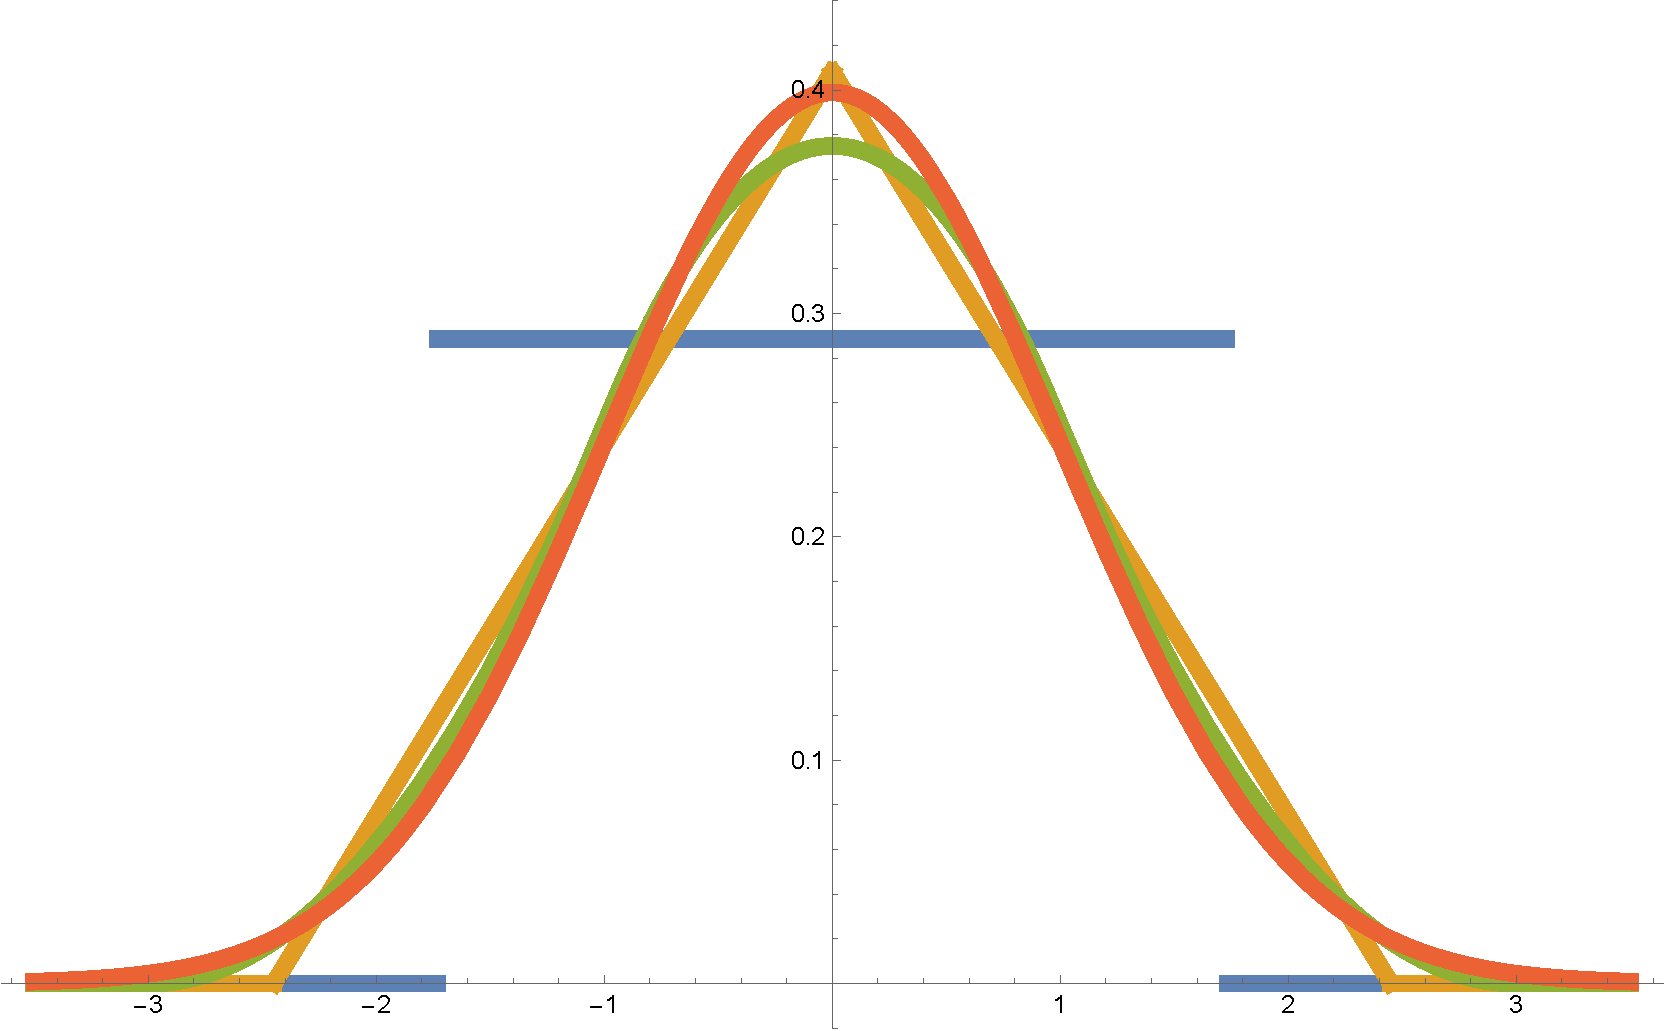
\includegraphics[width=0.5\textwidth]{./pictures/uniform_pdfs.pdf}
	\caption{Densities of $U_1$, $U_1+U_2$, $U_1+U_2+U_3$ (where $U_i$ are iid uniform on $[0,1]$),
		and $\mathcal{N}(0,1)$,
		normalized to have the same mean and variance.}
	\label{lecture1:fig:uniform_pdfs}
\end{figure}

\begin{example}
Let $\{X_i\}_{i=1}^{\infty}$ be a sequence of iid Bernoulli random variables with parameter $p$, meaning that each $X_i$ takes the value $1$ with probability $p$ and $0$ with probability $1 - p$. The mean and variance of each $X_i$ are given by:
\[
	\mu = \operatorname{\mathbb{E}}[X_i] = p, \quad \sigma^2 = \operatorname{\mathrm{Var}}(X_i) = p(1 - p).
\]
We also have the distribution of $X_1+\cdots+X_n$:
\begin{equation*}
	\operatorname{\mathbb{P}}\left( X_1+ \cdots + X_n = k \right) = \binom{n}{k} p^k (1-p)^{n-k},
	\qquad k = 0, 1, \ldots, n.
\end{equation*}

Introduce the normalized quantity
\begin{equation}
	\label{lecture1:eq:z_normalized_quantity}
	z = \frac{k - np}{\sqrt{np(1-p)}},
\end{equation}
and assume that throughout the asymptotic analysis,
this quantity stays finite.

Our aim is to show that, for $k$ such that $z$ remains bounded as $n\to\infty$, the following holds:
\[
\operatorname{\mathbb{P}}(S_n = k) = \frac{1}{\sqrt{2\pi np(1-p)}} \exp\Bigl( -\frac{z^2}{2} \Bigr) (1+o(1)).
\]

For large $n$, Stirling's formula gives
\[
m! \sim \sqrt{2\pi m}\, m^m e^{-m}, \quad \text{as } m\to\infty.
\]
Apply Stirling's approximation to $n!$, $k!$, and $(n-k)!$:
\[
n! \sim \sqrt{2\pi n}\, n^n e^{-n}, \quad
k! \sim \sqrt{2\pi k}\, k^k e^{-k}, \quad
(n-k)! \sim \sqrt{2\pi (n-k)}\,(n-k)^{n-k} e^{-(n-k)}.
\]
Thus,
\[
\binom{n}{k} \sim \frac{\sqrt{2\pi n}\, n^n e^{-n}}{\sqrt{2\pi k}\, k^k e^{-k}\sqrt{2\pi (n-k)}\,(n-k)^{n-k} e^{-(n-k)}}
= \frac{n^n}{k^k (n-k)^{n-k}}
\frac{1}{\sqrt{2\pi\, k(n-k)/n}}.
\]
More precisely, one often writes
\[
\binom{n}{k} \sim \frac{1}{\sqrt{2\pi np(1-p)}} \exp\Bigl( n\ln n - k\ln k - (n-k)\ln (n-k) \Bigr),
\]
where $p\approx k/n$ thanks to the fact that
$z$ \eqref{lecture1:eq:z_normalized_quantity} is assumed to be finite.

We have
\[
k = np+ z\sqrt{np(1-p)}.
\]
Then, consider the second-order Taylor expansion. We have
\[
n\ln n - k\ln k - (n-k)\ln (n-k) \sim n H -\frac{z^2}{2},
\]
where $H=-[p\ln p+(1-p)\ln(1-p)]+c(z;p)/\sqrt n$
(for an explicit function $c(z;p)$)
is the
``entropy'' term which exactly cancels with the prefactors coming from $p^k (1-p)^{n-k}$.

After combining the approximations from the binomial coefficient and the probability weights, one arrives at
\[
\operatorname{\mathbb{P}}(S_n = k)
\sim \frac{1}{\sqrt{2\pi np(1-p)}} \exp\left( -\frac{z^2}{2} \right),
\]
as desired.


(Note that this is a \emph{local} CLT as opposed to the convergence
\eqref{lecture1:eq:conv-in-dist} in the classical CLT; but one can get the latter
from the local CLT by integration.)

\end{example}


\subsection{Moments of the normal distribution}

\begin{proposition}
The moments of a random variable $Z \sim \mathcal{N}(0, \sigma^2)$ are given by:
\begin{equation}
	\label{lecture1:eq:normal-moments}
	\operatorname{\mathbb{E}}[Z^k] = \begin{cases}
		0, & \text{if } k \text{ is odd}, \\
		\sigma^k (k-1)!! = \sigma^k \cdot (k-1)(k-3) \cdots 1, & \text{if } k \text{ is even}.
	\end{cases}
\end{equation}
\end{proposition}
\begin{proof}
	We just compute the integrals. Assume $k$ is even (for odd,
	the integral is zero by symmetry). Also assume $\sigma = 1$ for simplicity.
	Then
\begin{equation*}
	\operatorname{\mathbb{E}}[Z^k]
	=
	\frac{1}{\sqrt{2\pi}}
	\int_{-\infty}^{\infty}  z^k e^{-z^2/2} \, dz.
\end{equation*}
Applying integration by parts (putting $ze^{-z^2/2}$ under $d$), we get
\begin{equation*}
	\operatorname{\mathbb{E}}[Z^k] = \frac{1}{\sqrt{2\pi}} \left[-z^{k-1}e^{-z^2/2}\right]_{-\infty}^{\infty} + \frac{k-1}{\sqrt{2\pi}} \int_{-\infty}^{\infty} z^{k-2} e^{-z^2/2} \, dz.
\end{equation*}
The first term vanishes at infinity (you can verify this using L'Hôpital's rule), leaving us with:
\begin{equation*}
	\operatorname{\mathbb{E}}[Z^k] = (k-1)\operatorname{\mathbb{E}}[Z^{k-2}].
\end{equation*}
This gives us a recursive formula, and completes the proof.
\end{proof}


\subsection{Moments of sums of iid random variables}

Let us now show the CLT by moments.
For example, the source is
\cite[Section~30]{billingsley1995probability}
or \cite{filmus2010two}.


\begin{remark}
	This proof requires an additional assumption
	that all moments of the random variables are finite.
	This is quite a strong assumption, and while the CLT holds
	without it, this proof by moments is more algebraic, and
	will translate to random matrices more directly.
\end{remark}

\subsubsection{Computation of moments}

Denote $Y_i=X_i-\mu$, these are also iid, but have mean $0$.
We consider
\begin{equation*}
	\operatorname{\mathbb{E}}\left[ \left( \sum_{i=1}^n Y_i \right)^k \right].
\end{equation*}
Expanding the $k$-th power using the multinomial theorem, we obtain:
\begin{equation*}
\left( \sum_{i=1}^n Y_i \right)^k = \sum_{j_1 + j_2 + \dots + j_n = k}
Y_{j_1} Y_{j_2} \dots Y_{j_n}.
\end{equation*}
Taking the expectation and using linearity, we have:
\begin{equation*}
 \mathbb{E}\left[ \left( \sum_{i=1}^n Y_i \right)^k \right]
 =
 \sum_{j_1 + j_2 + \dots + j_n = k}
 \operatorname{\mathbb{E}}\left[
	 Y_{j_1} Y_{j_2} \dots Y_{j_n}
 \right].
\end{equation*}
The sum over all $j_1, \ldots, j_n$ with $j_1 + \ldots + j_n = k$ is the number of ways to partition $k$ into $n$ non-negative integers.
We can order these integers, and thus
obtain the sum over all partitions of $k$ into $\le n$ parts.
Since $n$ is large, we simply sum over all partitions of $k$.
For each partition $\lambda$ of $k$
(where $k=\lambda_1+\lambda_2+\ldots+\lambda_n $ and
$\lambda_1\geq \lambda_2\geq \ldots\geq \lambda_n\geq 0$),
we must count the number of distinct multisets of indices
\((j_1,j_2,\ldots,j_n)\) that yield the same collection
\(\{\lambda_1,\lambda_2,\ldots\}\).
Then,
\begin{equation*}
	\operatorname{\mathbb{E}}\left[
		Y_{j_1} Y_{j_2} \dots Y_{j_n}
	\right]=
	\mathsf{m}_{\lambda_1}\mathsf{m}_{\lambda_2}\ldots \mathsf{m}_{\lambda_n},
\end{equation*}
where $\mathsf{m}_j=\mathbb{E}[Y^j]$ (recall the identical distribution of $Y_i$).
Note that
$\mathsf{m}_0 = 1$ and
$\mathsf{m}_1 = 0$.
Let us illustrate this with an
example.

\begin{example}
	For $k=4$, there are only two partitions
	which have no parts equal to $1$:
	$\lambda=(4)$ and $\lambda=(2,2)$.
	The number of ways to get $(4)$
	(so that
	$\operatorname{\mathbb{E}}[Y_{j_1} Y_{j_2} Y_{j_3} Y_{j_4}] = \mathsf{m}_4$)
	is to just
	assign one of the $j_p$ to be $4$,
	this can be done in $n$ ways.

	The number of ways to get $(2,2)$
	(so that
	$\operatorname{\mathbb{E}}[Y_{j_1} Y_{j_2} Y_{j_3} Y_{j_4}] = \mathsf{m}_2^2$)
	is to assign
	two of the $j_p$ to be $2$ and the other two to be $0$, this can be done in $\binom{n}{2}$ ways. Moreover,
	there are also 6 permutations of the indices
	$j_p=(i,j)$ which give the same partition $(2,2)$:
	$(i,i,j,j)$, $(j,j,i,i)$, $(i,j,i,j)$, $(j,i,j,i)$, $(i,j,j,i)$, $(j,i,i,j)$.
	Thus, the total number of ways to get $(2,2)$ is $6\binom{n}{2}\sim 3n^2$.

	So, we see that there is an $n$-dependent factor,
	and a ``combinatorial'' factor for each partition.
\end{example}

\subsubsection{$n$-dependent factor}
\label{lecture1:subsub:n-dependent-factor}

Consider first the $n$-dependent factor.
In the case $k$ is even and $\lambda=(2,2,\ldots,2 )$, the power
of $n$ is $n^{k/2}$.
In the case $k$ is even and $\lambda$ has at least one
part $\ge 3$, the power of $n$ is at most $n^{k/2-1}$,
which is subleading in the limit $n\to\infty$.
When $k$ is odd, the ``best'' we can do
(without parts equal to $1$)
is going to be
$\lambda=(3,2,\ldots, 2)$ with $(k-1)/2$ parts,
so the power of $n$ is $n^{(k-1)/2}$. This is also subleading
in the limit $n\to\infty$.


\subsubsection{Combinatorial factor}

Now, we see that we only need to consider the
case when $k$ is even and all parts of $\lambda$ are $2$.
Then, the $n$-dependent factor is $\binom{n}{k/2}\sim
n^{k/2}/(k/2)!$.
The combinatorial factor is
equal to the number of ways to partition $k$ into
pairs, which is the double factorial:
\begin{equation*}
	(k-1)!!=(k-1)(k-3)\ldots 1,
\end{equation*}
times the number of permutations
of the $k/2$ indices which are assigned to the pairs,
so $(k/2)!$.
In particular, for $k=4$ this is $6$.

\subsubsection{Putting it all together}

We have as $n\to\infty$:
\begin{equation*}
	\mathbb{E}\left[ \left( \sum_{i=1}^n Y_i \right)^k \right]
	=
	n^{k/2}
	\frac{(k-1)!!}{(k/2)!}\cdot (k/2)!
	\sigma^k
	+o(n^{k/2})=
	n^{k/2}
	(k-1)!!
	\sigma^k
	+o(n^{k/2}).
\end{equation*}

Now, we need to consider the normalization of the sum
$\sum_{i=1}^n Y_i$ by $\sqrt{n}$:
\begin{equation*}
	\mathbb{E}\left[ \left( \frac{1}{\sqrt{n}} \sum_{i=1}^n Y_i \right)^k \right]
	=
	\frac{1}{n^{k/2}}
	\mathbb{E}\left[ \left( \sum_{i=1}^n Y_i \right)^k \right]
	=
	(k-1)!!
	\sigma^k
	+o(1).
\end{equation*}
Therefore, the moments of
$Z_n$ \eqref{lecture1:eq:normalized-sum}
converge to the moments of the standard normal distribution.


\subsection{Convergence in distribution}

Is convergence of moments enough to imply convergence in
distribution? Not necessarily. First, note that the functions
$x\mapsto x^k$ are not even bounded on $\mathbb{R}$.

A sufficient condition for convergence in distribution is
found in the
classical method of moments in
probability theory \cite[Theorem~30.2]{billingsley1995probability}.
This theorem
states that
if the limiting distribution $X$ is uniquely determined by its moments,
then convergence in moments implies convergence in distribution.

The normal distribution is indeed uniquely determined by its
moments (Problem \ref{lecture1:prob:uniqueness-normal}),
so the CLT holds in this case, provided that the
original iid random variables $X_i$ have finite moments of
all orders.

\section{Random matrices and semicircle law}

We now turn to random matrices.

\subsection{Where can randomness in a matrix come from?}


The study of random matrices begins with understanding how randomness can be introduced into matrix structures. We consider three primary sources:
\begin{enumerate}
\item \textbf{iid entries:}
The simplest form of randomness comes from filling matrix entries independently with samples from a fixed probability distribution. For an $n \times n$ matrix, this gives us $n^2$ independent random variables.
If we do not impose any additional structure on the matrix, then the eigenvalues
will be complex. So, often we consider real symmetric, complex Hermitian, or quaternionic matrices with
symplectic symmetry.\footnote{Real symmetric means $A^\top=A$, complex Hermitian means $A^\dagger=A$ (conjugate transpose).
	Let us briefly discuss the quaternionic case. It can be modeled over $\mathbb{C}$. A quaternion
	$q = a + b\,\mathbf{i} + c\,\mathbf{j} + d\,\mathbf{k}$
	can be represented by the complex $2\times 2$ matrix
	\[
	q \;\longmapsto\;
	\begin{pmatrix}
	a + \mathbf{i}b & c + \mathbf{i}d \\
	-c + \mathbf{i}d & a - \mathbf{i}b
	\end{pmatrix}.
	\]
	The entries $a,b,c,d$ for the quaternion matrix case must be real, and the matrix
$A$ of size $2n\times 2n$ should also be Hermitian in the usual complex sense.\label{lecture1:fn:quaternion}}


\item \textbf{Correlated entries:}
In many physical systems, especially those modeling local interactions, matrix entries are not independent but show correlation patterns. Common examples include:
\begin{itemize}
\item Band matrices, where entries become negligible far from the diagonal
\item Matrices with correlation decay based on the distance between indices
\item Structured random matrices arising from specific physical models
\item Sparse matrices, where most entries are zero
\end{itemize}
\item \textbf{Haar measure on matrix groups:}
Randomness can come from considering matrices sampled according to the Haar measure on a compact matrix group,
for example, the orthogonal $O(n)$, unitary $U(n)$, or symplectic group $Sp(n)$.\footnote{The
	orthogonal and unitary groups are defined
	in the usual way, by $OO^\top=O^\top O=I$ and $UU^\dagger
	=U^\dagger U=I$, respectively.
	The
	group $Sp(n)$ is the compact real form of the full symplectic group $Sp(2n, \mathbb{C})$,
	consisting of $2n\times 2n$ matrices $A$ such that $A^\top JA=J$, where
	$J$ is the skew-symmetric form.}
One can think of this as a generalization of
the uniform distribution (Lebesgue measure) on the unit circle in $\mathbb{C}$,
or a unit sphere in $\mathbb{R}^n$.
One can also mix and match: one
of the most interesting families of random matrices is the one
with constant eigenvalues, but random eigenvectors:
\begin{equation*}
	A=UD_\lambda U^\dagger,\qquad U\in U(n), \quad U\sim \mathrm{Haar}.
\end{equation*}
Here $D_\lambda$ is a diagonal matrix with constant eigenvalues $\lambda=(\lambda_1,\ldots,\lambda_n)$.
The random matrix $A$ is the ``uniform'' random variable
taking values in the set of all Hermitian matrices with fixed real eigenvalues $\lambda$.
Here we may assume that $\lambda_1\ge \ldots\ge \lambda_n $,
since the unitary conjugation can permute the eigenvalues.
\end{enumerate}

\subsection{Real Wigner matrices}


\begin{definition}[Real Wigner Matrix]
An $n \times n$ random matrix $W=W_n = (X_{ij})_{1 \leq i,j \leq n}$ is called a \emph{real Wigner matrix} if:
\begin{enumerate}
    \item $W$ is symmetric: $X_{ij} = X_{ji}$ for all $i,j$;
    \item The upper triangular entries $\{X_{ij}: 1 \leq i \leq j \leq n\}$ are independent;
    \item The diagonal entries $\{X_{ii}\}$ are iid real random variables with mean $0$ and variance $\sigma_d$;
    \item The upper triangular entries $\{X_{ij}: i < j\}$ are iid
			(possibly with a distribution different from the diagonal entries) real random variables
			with mean $0$ and variance $\sigma$;
		\item (optional, but we assume this) All entries have finite moments of all orders.
\end{enumerate}
\end{definition}

\begin{example}[Gaussian Wigner Matrices, Gaussian Orthogonal Ensemble (GOE)]
Let $W$ be a real Wigner matrix where:
\begin{itemize}
    \item Diagonal entries $X_{ii} \sim \mathcal{N}(0, 2)$;
		\item Upper triangular entries $X_{ij} \sim \mathcal{N}(0, 1)$ for $i < j$.
\end{itemize}
We can model $W$ as $(Y+Y^\top)/\sqrt{2}$,
where $Y$ is a matrix with iid Gaussian entries $Y_{ij} \sim \mathcal{N}(0, 1)$.
The matrix distribution of $W$ is called
the \emph{Gaussian Orthogonal Ensemble} (\emph{GOE}).
\end{example}

\begin{remark}[Wishart Matrices]
	\label{lecture1:rmk:wishart-matrices}
	There are other ways to define random matrices,
	most notably, \emph{sample covariance matrices}.
	Let $A = [a_{i,j}]_{i,j=1}^{n,m}$ be an $n \times m$ matrix ($n \leq m$), where entries are iid real random variables with
	mean $0$ and finite variance.
	Then $M = AA^\top$ is a positive symmetric random matrix of
	size $n \times n$. It almost surely has full rank.
\end{remark}


\subsection{Empirical spectral distribution}

For an arbitrary random matrix of size $n\times n$ with real eigenvalues,
the \emph{empirical spectral distribution} (\emph{ESD}) is defined as the
random probability measure on $\mathbb{R}$:
\begin{equation}
	\label{lecture1:eq:esd-defintion}
	\mu_n = \frac{1}{n} \sum_{i=1}^n \delta_{\lambda_i},
\end{equation}
which puts point masses of size $1/n$ at the eigenvalues $\lambda_i$ of the matrix.

If you sample the ESD for a large real Wigner matrix,
and take a histogram (to cluster the eigenvalues into boxes),
you will see the semi-circular pattern. This pattern
does not change over several samples. Hence, one can
conjecture that the
ESD \eqref{lecture1:eq:esd-defintion} converges to a nonrandom
measure, after rescaling.

We can guess the rescaling by looking at the first two moments of the ESD.
The first moment is
\begin{equation}
	\label{lecture1:eq:first-moment-esd}
	\int_{\mathbb{R}} x \, \mu_n(dx) = \frac{1}{n} \sum_{i=1}^n \lambda_i=
	\frac{1}{n} \operatorname{Tr}(W) =
	\frac{1}{n}\sum_{i=1}^n X_{ii},
\end{equation}
and this sum has mean zero (and small variance), so it converges to zero.
The second moment is
\begin{equation}
	\label{lecture1:eq:second-moment-esd}
	\int_{\mathbb{R}} x^2 \, \mu_n(dx) = \frac{1}{n} \sum_{i=1}^n \lambda_i^2=
	\frac{1}{n} \operatorname{Tr}(W^2) =
	\frac{1}{n}
	\sum_{i,j=1}^n X_{ij}^2.
\end{equation}
This sum has mean $\sim \sigma^2 n^2$, so even normalized by $n$,
it still goes to infinity.
But, if we normalize the matrix as $\frac{1}{\sqrt n}W$,
then the second moment
becomes bounded, and one can convince oneself that the
ESD of the normalized Wishart matrix has a limit.
Indeed, this is the case:

\begin{theorem}[Wigner's Semicircle Law]
	\label{lecture1:thm:esd-semicircle}
	Let $W$ be a real Wigner matrix of size $n\times n$
	(with off-diagonal entries having a fixed variance $\sigma^2$, independent of $n$).
	Then
	as $n\to\infty$,
	the ESD of $W/(\sigma\sqrt{n})$ converges in distribution to the semicircular law:
	\begin{equation}
		\label{lecture1:eq:thm-esd-semicircle}
		\nu_n\coloneqq \frac{1}{n}\sum_{i=1}^{n}\delta_{\lambda_i/\sqrt{n}}
		\longrightarrow \mu_{\mathrm{sc}},
	\end{equation}
	where $\mu_{\mathrm{sc}}$ is the semicircular distribution with density
	with respect to the Lebesgue measure:
	\begin{equation}
		\label{lecture1:eq:semicircle-density-defintion}
		\mu_{\mathrm{sc}}(dx) \coloneqq \frac{1}{2\pi} \sqrt{4-x^2} \ssp \mathbf{1}_{|x| \leq 2}\ssp
		dx.
	\end{equation}
\end{theorem}

\begin{remark}
	The convergence in \eqref{lecture1:eq:thm-esd-semicircle} may mean either
	\emph{weakly in probability} or \emph{weakly almost surely}.
	The first notion, weak convergence in probability, means that
	for every bounded continuous function $f$,
	we have
	\begin{equation}
		\label{lecture1:eq:weak-convergence-in-prob}
		\int_{\mathbb{R}} f(x) \, \nu_n(dx) \longrightarrow \int_{\mathbb{R}} f(x) \, \mu_{\mathrm{sc}}(dx),\qquad  n\to\infty,
	\end{equation}
	where in \eqref{lecture1:eq:weak-convergence-in-prob} the convergence is in probability.
	Indeed, the left-hand side of \eqref{lecture1:eq:weak-convergence-in-prob}
	is a random variable, so we need to qualify which sense of convergence we mean.

	The weakly almost sure convergence means that
	the convergence in \eqref{lecture1:eq:weak-convergence-in-prob}
	holds for almost all realizations of the random matrix $W$,
	that is, for every bounded continuous function $f$,
	the random variable
	$\int_{\mathbb{R}} f(x) \, \nu_n(dx)$ converges almost surely to
	$\int_{\mathbb{R}} f(x) \, \mu_{\mathrm{sc}}(dx)$.
\end{remark}

\begin{remark}
	There exists a version of the limiting
	ESD for the Wishart matrices
	(\Cref{lecture1:rmk:wishart-matrices}).
	In this case, the limiting distribution is the
	\emph{Marchenko-Pastur law}
	\cite{MarchenkoPastur}.
\end{remark}

\subsection{Expected moments of traces of random matrices}

The main computation in the proof of
\Cref{lecture1:thm:esd-semicircle} is the computation of
expected moments of the ESD.
This computation of moments is somewhat similar
to the one in the proof of the CLT by moments,
but has its own random matrix flavor.

\begin{definition}[Normalized Moments]
For each $k\geq 1$, the normalized $k$-th moment of the empirical spectral distribution of $W_n/\sqrt{n}$ is given by
\[
m_k^{(n)}=\int_{\mathbb{R}} x^k\,\nu_n(dx)
=\frac{1}{n^{k/2+1}}\operatorname{Tr}(W^k).
\]
\end{definition}
Our first goal is to study the asymptotic behavior of
$\operatorname{\mathbb{E}}[m_k^{(n)}]$ as $n\to\infty$ for each fixed
$k\geq 1$, just like we did in
\eqref{lecture1:eq:first-moment-esd}--\eqref{lecture1:eq:second-moment-esd}
for $k=1,2$:
\begin{equation*}
	\operatorname{\mathbb{E}}[m_1^{(n)}] = 0, \qquad
	\operatorname{\mathbb{E}}[m_2^{(n)}] \to \sigma^2.
\end{equation*}
Note that $\operatorname{\mathbb{E}}[m_2^{(n)}]$
is not exactly equal to $\sigma^2$ because of the presence of the
diagonal elements which have a different distribution.
In general, we will see that the contribution
of the diagonal elements to the moments is negligible
in the limit $n\to\infty$.

\begin{lemma}[Convergence of Expected Moments]
\label{lecture1:lemma:moments_convergence}
For each fixed $k \geq 1$, we have
\[
\lim_{n \to \infty} \operatorname{\mathbb{E}}[m_k^{(n)}] =
\begin{cases}
0 & \text{if $k$ is odd}, \\
\sigma^k C_{k/2} & \text{if $k$ is even},
\end{cases}
\]
where $C_m = \frac{1}{m+1}\binom{2m}{m}$ is the $m$-th Catalan number.
\end{lemma}

The even moments are scaled by powers of $\sigma$ just as in the case $k=2$,
while the odd moments vanish due to the symmetry of the limiting distribution
around zero.
As we will see, the appearance of Catalan numbers is not accidental,
but it is due to the underlying combinatorics.

\begin{proof}[Proof of \Cref{lecture1:lemma:moments_convergence}]
	The trace of $W^k$ expands as a sum over all possible index sequences:
	\begin{equation}
		\operatorname{Tr}(W^k) = \sum_{i_1,\ldots,i_k=1}^n X_{i_1i_2}X_{i_2i_3}\cdots X_{i_{k-1}i_k}X_{i_ki_1}.
	\end{equation}
	Due to independence and the fact that
	$\mathbb{E}[X_{ij}]=0$ for all $i,j$, the only nonzero
	contributions come from index sequences
	where each matrix element appears least twice.

	As in the CLT proof, there is a power-$n$ factor and a combinatorial factor.

	For $k$ odd, let us count the power of $n$ first. As
	in the CLT proof, the
	maximum power comes from index sequences where all matrix
	elements appear exactly twice except for one which appears
	three times. Indeed, this corresponds to the maximum
	freedom of choosing $k$ indices among the large number $n$
	of indices, and thus to the maximum power of $n$.
	This maximum power of $n$ is $n^{1+\lfloor k/2 \rfloor }$
	(note that there is an extra factor $n$ compared to the CLT proof,
	as now we have $\sim n^2$ random variables in the matrix instead of $n$).
	Since this is strictly less than the
	normalization $n^{k/2+1}$ in $m_k^{(n)}$, the term with odd $k$
	vanish in the limit $n\to\infty$.

	Assume now that $k$ is even.
	Then the maximum power of $n$ comes from index sequences where each matrix element appears exactly twice.
	This power of $n$ is $n^{k/2+1}$, which exactly
	matches the normalization in $m_k^{(n)}$.

	It remains to count the combinatorial factor,
	assuming that $k$ is even.
	For each term in the trace expansion, we can represent the sequence of indices $(i_1,\ldots,i_k)$ as a directed closed path with vertices $\{1,\ldots,n\}$ and edges given by the matrix entries $X_{i_ai_{a+1}}$. For example, if $k=4$ and we have a term $X_{12}X_{23}X_{34}X_{41}$, this corresponds to the path $1\to 2\to 3\to 4\to 1$. Recall that our path must have each
	matrix entry exactly twice (within the symmetry $X_{ij}=X_{ji}$),
	and the path must be closed.
	The condition that each edge appears exactly twice
	means that if we forget the direction of the edges and the multiplicities,
	we must get a \emph{tree}, with $k/2$ edges and $k/2+1$ vertices.
	The complete justification of this counting is the
	problem in Problem \ref{lecture1:prob:counting-n-powers}.

	The $n$-powers counting implies that the combinatorial
	factor (for even $k$)
	is equal to $\sigma^k$ times the
	number of \emph{rooted} (\emph{planar}) \emph{trees} with $k/2$ edges.
	The rooted condition comes from the fact that
	we are free to fix the starting point of the path
	to be $1$ (this ambiguity is taken into account by the
	power-$n$ factor).

	In Problem \ref{lecture1:prob:counting-trees}, we show that the number of these rooted trees is the $k/2$-th Catalan number $C_{k/2}$.
	This completes the proof of \Cref{lecture1:lemma:moments_convergence}.
\end{proof}

\subsection{Immediate next steps}

The proof of \Cref{lecture1:thm:esd-semicircle} is continued in the next
\Cref{chap:lecture2}.
Immediate next steps are:
\begin{enumerate}
	\item Show that the number of rooted trees with $k/2$ edges is the $k/2$-th Catalan number, and give the exact formula for the Catalan numbers.
	\item Compute the moments of the semicircular distribution.
	\item Make sure that the moment computation suffice to show the
		weak in probability convergence of the ESD to the semicircular law.
\end{enumerate}





\section{Problems}

Each problem is a subsection (like Problem \ref{lecture1:prob:normal-approximation}),
and may have several parts.

\subsection{Normal approximation}
\label{lecture1:prob:normal-approximation}

\begin{enumerate}
	\item In \Cref{lecture1:fig:uniform_pdfs}, which color is
		the normal curve and which is the sum of three uniform random variables?
	\item Show that the sum of 12 iid uniform random variables on $[-1,1]$
		(without normalization) is approximately standard normal.
	\item Find (numerically is okay)
		the maximum discrepancy between the distribution of the sum of 12 iid uniform random variables on $[-1,1]$ and the standard normal distribution:
		\begin{equation*}
			\sup_{x \in \mathbb{R}} \left| \operatorname{\mathbb{P}}\left(  \sum_{i=1}^{12} U_i \leq x \right) - \operatorname{\mathbb{P}}\left( Z \leq x \right) \right|.
		\end{equation*}
\end{enumerate}

\subsection{Convergence in distribution}
\label{lecture1:prob:conv-in-dist-problem}

Convergence in distribution $X_n\to X$
for real random variables $X_n$ and $X$ means, by definition,
that
\begin{equation*}
	\operatorname{\mathbb{E}}[f(X_n)] \to \operatorname{\mathbb{E}}[f(X)]
\end{equation*}
for all bounded continuous functions $f$.
Show that convergence in distribution
is equivalent to the condition outlined in \eqref{lecture1:eq:conv-in-dist}:
\begin{equation*}
	\lim_{n \to \infty} \operatorname{\mathbb{P}}(X_n \leq x) = \operatorname{\mathbb{P}}(X \leq x)
\end{equation*}
for all $x$ at which the cumulative distribution function of $X$ is continuous.

\subsection{Moments of sum justification}

Justify the computations of the power of $n$ in
\Cref{lecture1:subsub:n-dependent-factor}.

\subsection{Distribution not determined by moments}

Show that the log-normal random variable
$e^{Z}$ (where $Z\sim \mathcal{N}(0,1)$)
is not determined by its moments.

\subsection{Uniqueness of the normal distribution}
\label{lecture1:prob:uniqueness-normal}

Show that the normal distribution is uniquely determined by its moments.

\subsection{Quaternions}

Show that the $2\times 2$ matrix representation of a quaternion
given in Footnote~\ref{lecture1:fn:quaternion}
indeed satisfies the quaternion multiplication rules.
Hint: Use linearity and distributive law.

\subsection{Ensemble $UD_\lambda U^\dagger$}

Let $U$ be the random Haar-distributed unitary matrix of size $N\times N$.
Let $D_\lambda$ be the diagonal matrix with constant real eigenvalues
$\lambda=(\lambda_1,\ldots,\lambda_N)$,
$\lambda_1\ge \ldots\ge \lambda_N$.
Let us fix $\lambda$ to be, say, $\lambda=(1,1,\ldots,1,0,0,\ldots,0  )$,
for some proportion of $1$'s and $0$'s (you can start with half
ones and half zeros).

Use a computer algebra system to
sample the eigenvalues of the matrix
obtained from $UD_\lambda U^\dagger$
by taking only its top-left corner of size $k\times k$,
where $k=1,2,\ldots,N $.
For a fixed $k$, let
$\lambda_1^{(k)}\ge \ldots\ge \lambda_k^{(k)}$
be the eigenvalues of the top-left corner of size $k\times k$.
Plot the two-dimensional array
\begin{equation*}
	\left\{ (\lambda_i^{(k)},k)\colon i=1,\ldots,k,\ k=1,\ldots,N  \right\}\subset \mathbb{R}\times
	\mathbb{Z}_{\ge1}.
\end{equation*}

\subsection{Invariance of the GOE}

Show that the distribution of the GOE is invariant under
conjugation by orthogonal matrices:
\begin{equation*}
	\operatorname{\mathbb{P}}(O W O^\top \in \mathrm{A}) = \operatorname{\mathbb{P}}(W \in \mathrm{A})
\end{equation*}
for all orthogonal matrices $O$ and Borel sets $\mathrm{A}$.

\subsection{Counting $n$-powers in the real Wigner matrix}
\label{lecture1:prob:counting-n-powers}

Show that in the expansion of the expected trace of the
$k$-th power of the real Wigner matrix, the maximum power of
$n$ is $k/2+1$ for even $k$ and less for odd $k$. For even
$k$, the power $k/2+1$ comes from index sequences where each
off-diagonal matrix element appears exactly twice, and no
diagonal elements are present.





\subsection{Counting trees}
\label{lecture1:prob:counting-trees}

Show that the number of rooted trees with $m$ edges is the $m$-th Catalan number:
\begin{equation*}
	C_m = \frac{1}{m+1}\binom{2m}{m}.
\end{equation*}

















\chapter{Wigner semicircle law}
\label{chap:lecture2}







\begin{lnotes}
	PREP:
	\begin{enumerate}
		\item Start:
			Catalan number formula
		\item Moments of SC need to be computed
		\item
			SC is uniquely determined by its moments; need Carleman criterion to show that the moments determine the distribution.
		\item from expected moments to the full convergence, some analysis needed
	\end{enumerate}
\end{lnotes}


\section{Recap}

We are working on the Wigner semicircle law.
\begin{enumerate}
	\item Wigner matrices $W$:
		real symmetric random matrices with iid entries
		$X_{ij}$, $i>j$ (mean 0, variance $\sigma^2$);
		and iid diagonal entries $X_{ii}$ (mean 0, some other variance and distribution).
	\item Empirical spectral distribution (ESD)
		\begin{equation*}
			\nu_n = \frac{1}{n} \sum_{i=1}^{n} \delta_{\lambda_i/\sqrt{n}},
		\end{equation*}
		which is a random probability measure on $\mathbb{R}$.
	\item Semicircle distribution $\mu_{\mathrm{sc}}$:
		\begin{equation*}
			\mu_{\mathrm{sc}}(dx) = \frac{1}{2\pi} \sqrt{4-x^2} \, dx,
			\qquad x \in [-2,2].
		\end{equation*}
	\item Computation of expected traces of powers of $W$
		(with variance $1$). We
		showed that
		\begin{equation*}
		\int_{\mathbb{R}} x^k \, \nu_n(dx) \to
			\#\left\{ \textnormal{rooted planar trees with $k/2$ edges} \right\}.
		\end{equation*}
\end{enumerate}

\begin{remark}
	If the off-diagonal elements of the matrix have variance $\sigma^2$, then the
	semicircle distribution should be scaled to be supported on $[-2\sigma,2\sigma]$.
	We assume that the variance of the off-diagonal elements is $1$
	in most arguments throughout the lecture.
\end{remark}

\section{Two computations}

First, we finish the combinatorial part,
and match the limiting expected traces of powers of $W$
to moments of the semicircle law.

\subsection{Moments of the semicircle law}

We also need to match the Catalan numbers to the moments of the semicircle law.
Let $k=2m$, and we need to compute
the integral
\begin{equation*}
	\int_{-2}^{2} x^{2m} \frac{1}{2\pi} \sqrt{4-x^2} \, dx.
\end{equation*}

By symmetry, we write:
\[
\int_{-2}^2 x^{2m}\rho(x)\, dx = \frac{2}{\pi} \int_0^2 x^{2m} \sqrt{4-x^2}\, dx.
\]

Using the substitution \(x = 2\sin\theta\), we have \(dx = 2\cos\theta\, d\theta\). The integral becomes:
\[
\frac{2}{\pi} \int_0^{\pi/2} (2\sin\theta)^{2m} (2\cos\theta) (2\cos\theta\, d\theta)
= \frac{2^{2m+2}}{\pi} \int_0^{\pi/2} \sin^{2m}\theta \cos^2\theta\, d\theta.
\]
Using \(\cos^2\theta = 1 - \sin^2\theta\), we split the integral:
\[
\frac{2^{2m+2}}{\pi} \left( \int_0^{\pi/2} \sin^{2m}\theta\, d\theta - \int_0^{\pi/2} \sin^{2m+2}\theta\, d\theta \right).
\]
Using the standard formula (cf. Problem \ref{lecture2:prob:sin-integral})
\begin{equation}
	\label{lecture2:eq:sin-integral}
\int_0^{\pi/2} \sin^{2n}\theta\, d\theta = \frac{\pi}{2} \frac{(2n)!}{2^{2n} (n!)^2},
\end{equation}
we compute each term:
\[
\frac{2^{2m+2}}{\pi} \left( \frac{\pi}{2} \frac{(2m)!}{2^{2m}(m!)^2} - \frac{\pi}{2} \frac{(2m+2)!}{2^{2m+2}((m+1)!)^2} \right).
\]
After simplification, this becomes
$C_m$, the $m$-th Catalan number.

\subsection{Counting trees and Catalan numbers}

Throughout this section, for a random matrix trace moment of order $k$,
we use $m=k/2$ as our main parameter. Note that $m$ can be arbitrary
(not necessarily even).

\begin{definition}[Dyck Path]
A \emph{Dyck path} of semilength $m$ is a sequence of $2m$ steps in the plane, each step being either $(1,1)$ (up step) or $(1,-1)$ (down step), starting at $(0,0)$ and ending at $(2m,0)$, such that the path never goes below the $x$-axis. We denote an up step by $U$ and a down step by $D$.
\end{definition}

\begin{definition}[Rooted Plane Tree]
A \emph{rooted plane tree} is a tree with a designated root vertex where the children of each vertex have a fixed left-to-right ordering. The size of such a tree is measured by its number of edges, which we denote by $m$.
\end{definition}

\begin{definition}[Catalan Numbers]
The sequence of \emph{Catalan numbers} $\{C_m\}_{m\geq 0}$ is defined recursively by:
\begin{equation}
	\label{lecture2:eq:catalan-recurrence}
    C_0 = 1, \quad C_{m+1} = \sum_{j=0}^m C_j C_{m-j} \quad \text{for } m \geq 0.
\end{equation}
Alternatively, they have the closed form\footnote{See
	Problem \ref{lecture2:prob:reflection-principle} for a combinatorial proof
of the second inequality.}
\begin{equation}
	\label{lecture2:eq:catalan-closed}
    C_m = \frac{1}{m+1}\binom{2m}{m} =
		\binom{2m}{m} - \binom{2m}{m+1}.
\end{equation}
These numbers appear naturally in the moments of random matrices, where $m=k/2$ for trace moments of order $k$.
\end{definition}

\begin{lemma}
	\label{lecture2:lemma:equivalence-catalan}
	Formulas
	\eqref{lecture2:eq:catalan-recurrence} and \eqref{lecture2:eq:catalan-closed} are equivalent.
\end{lemma}
\begin{proof}
	One can check that the closed form satisfies the recurrence relation by direct substitution. The other direction
	involves generating functions. Namely,
	\eqref{lecture2:eq:catalan-recurrence} can be rewritten for the
	generating function
	\begin{equation*}
		C(z)=\sum_{m=0}^\infty C_m z^m
	\end{equation*}
	as
	\begin{equation*}
		C(z)=1+zC(z)^2.
	\end{equation*}
	Solving for $C(z)$, we get
	\begin{equation}
		\label{lecture2:eq:catalan-generating}
		C(z)=\frac{1\pm \sqrt{1-4z}}{2z}.
	\end{equation}
	We need to pick the solution which is nonsingular at $z=0$,
	and it corresponds to the minus sign.
	Taylor expansion of the right-hand side of
	\eqref{lecture2:eq:catalan-generating}
	at $z=0$
	gives the closed form.
\end{proof}

\begin{remark}
	\label{lecture2:rmk:stanley-catalans}
	Catalan numbers enumerate many (too many!) combinatorial objects. For a comprehensive treatment, see \cite{stanley2015catalan}.
\end{remark}

\begin{proposition}[Dyck Path--Rooted Tree Correspondence]
	\label{lecture2:prop:dyck-tree}
For any $m$, there exists a bijection between
the set of Dyck paths of semilength $m$ and the set of rooted plane trees with $m$ edges.
\end{proposition}

\begin{proof}
Given a Dyck path of semilength $m$, we build the corresponding rooted plane tree as follows
(see \Cref{lecture2:fig:dyck_paths_m2} for an illustration):
\begin{enumerate}
    \item Start with a single root vertex
    \item Read the Dyck path from left to right:
        \begin{itemize}
            \item For each up step ($U$), add a new child to the current vertex
            \item For each down step ($D$), move back to the parent of the current vertex
        \end{itemize}
    \item The order of children is determined by the order of up steps
\end{enumerate}
This is clearly a bijection, and we are done.
\end{proof}


\begin{figure}[htpb]
\centering
\begin{tikzpicture}[scale=0.8]
    % First Dyck path (UUDD)
    \begin{scope}[xshift=0cm]
        % Grid
        \draw[help lines,gray!30] (0,0) grid[step=1] (4,2);
        \draw[->,gray!50] (-0.2,0) -- (4.2,0) node[right] {$x$};
        \draw[->,gray!50] (0,-0.2) -- (0,2.2) node[above] {$y$};

        % Path
        \draw[thick,blue] (0,0) -- (1,1) -- (2,2) -- (3,1) -- (4,0);

        % Label
        \node[below] at (2,-0.5) {UUDD};
    \end{scope}

    % First tree
    \begin{scope}[xshift=6cm,level distance=1cm,
        every node/.style={circle,draw,minimum size=0.5cm}]
        \node (a) {1}
            child {node (b) {2}
                child {node (c) {3}}
            };
    \end{scope}

    % Second Dyck path (UDUD)
    \begin{scope}[xshift=10cm]
        % Grid
        \draw[help lines,gray!30] (0,0) grid[step=1] (4,2);
        \draw[->,gray!50] (-0.2,0) -- (4.2,0) node[right] {$x$};
        \draw[->,gray!50] (0,-0.2) -- (0,2.2) node[above] {$y$};

        % Path
        \draw[thick,red] (0,0) -- (1,1) -- (2,0) -- (3,1) -- (4,0);

        % Label
        \node[below] at (2,-0.5) {UDUD};
    \end{scope}

    % Second tree
    \begin{scope}[xshift=16cm,level distance=1cm,
        every node/.style={circle,draw,minimum size=0.5cm}]
        \node (a) {1}
            child {node (b) {2}}
            child {node (c) {3}};
    \end{scope}
\end{tikzpicture}
\caption{The two possible Dyck paths of semilength $m=2$ and their corresponding rooted plane trees.}
\label{lecture2:fig:dyck_paths_m2}
\end{figure}

It remains to show that the Dyck paths or rooted plane trees are counted by the Catalan numbers, by verifying
the recursion \eqref{lecture2:eq:catalan-recurrence} for them.
By \Cref{lecture2:prop:dyck-tree}, it suffices to
consider only Dyck paths.

\begin{proposition}
	\label{lecture2:prop:dyck-recurrence}
	The number of Dyck paths of semilength $m$ satisfies the Catalan recurrence \eqref{lecture2:eq:catalan-recurrence}.
\end{proposition}
\begin{proof}
	We need to show that the number of Dyck paths of semilength $m+1$ is given by the sum in the right-hand side of \eqref{lecture2:eq:catalan-recurrence}.
	Consider a Dyck path of semilength $m+1$,
	and let the \emph{first} time it
	returns to zero be at semilength $j+1$,
	where $j=0,\ldots,m$.
	Then the
	first and the $(2j+1)$-st steps are,
	respectively, $U$ and $D$.
	From $0$ to $2j+2$, the path does not return to the $x$-axis,
	so we can remove the first and the $(2j+1)$-st steps, and get a proper Dyck path of semilength $j$.
	The remainder of the Dyck path is a Dyck path of semilength $m-j$.
	This yields the desired recurrence.
\end{proof}
\begin{figure}[htbp]
	\centering
	\begin{tikzpicture}[scale=0.8]
		% Drawing the Dyck path with highlighted portions
		\draw[thick] (0,0) -- (1,1) -- (2,2) -- (3,1) -- (4,2) -- (5,1) -- (6,0)
		-- (7,1) -- (8,0)--++(1,1)--++(1,1)--++(1,-1)--++(1,-1)--++(1,1)--++(1,-1);

		% Axes and labels
		\draw[->] (-0.5,0) -- (16.5,0) node[right] {$x$};
		\draw[->] (0,-0.5) -- (0,4.5) node[above] {$y$};


		% Highlight important steps for recurrence explanation
		\draw[line width=2pt,red] (0,0) -- (1,1);
		\draw[line width=2pt,red] (5,1) -- (6,0);
	\end{tikzpicture}
	\caption{Illustration of a Dyck path decomposition for the proof of \Cref{lecture2:prop:dyck-recurrence}.}
	\label{lecture2:fig:dyck_recurrence}
\end{figure}


\section{Analysis steps in the proof}

We are done with combinatorics, and it remains to justify that
the computations lead to the desired semicircle law
from \Cref{chap:lecture1}.

Let us remember that so far, we showed that
\begin{equation*}
	\lim_{n\to\infty}
	\frac{1}{n^{k/2+1}}
	\operatorname{\mathbb{E}}
	\left[
		\operatorname{Tr} W^k
	\right]
	=
	\begin{cases}
		\sigma^{2m} C_{m} & \text{if $k=2m$ is even}, \\
		0 & \text{if $k$ is odd}.
	\end{cases}
\end{equation*}
Here, $W$ is real Wigner
(unnormalized) with mean $0$,
where its off-diagonal entries are iid with variance $\sigma^2$.

\subsection{The semicircle distribution is determined by its moments}
\label{lecture2:sub:carleman-semicircle}

We use (without proof)
the known Carleman's criterion for the uniqueness of a distribution by its moments.
\begin{proposition}[Carleman's criterion
	{\cite[Theorem~1.10]{shohat1943problem}}, \cite{Akhiezer1965Moment}]
	\label{lecture2:prop:carleman}
	Let $X$ be a real-valued random variable with moments $m_k
	= \mathbb{E}[X^k]$ of all orders. If
	\begin{equation}
		\label{lecture2:eq:Carleman}
		\sum_{k=1}^{\infty}
		(m_{2k})^{-1/(2k)} = \infty,
	\end{equation}
	then the distribution of
	$X$ is uniquely determined by its moments $(m_k)_{k\geq 1}$.
\end{proposition}
\begin{remark}
Note that we do not assume that the measure is symmetric,
but use only even moments for the Carleman criterion.
Indeed,
in determining uniqueness, the decisive aspect is how the
distribution mass ``escapes'' to \(\pm \infty\). Since
\(\int |x|^n d\mu(x)\) can be bounded by twice \(\int x^{2
\lfloor n/2 \rfloor} d\mu(x)\) (roughly speaking),
controlling \(\int x^{2n} d\mu(x)\) also controls \(\int
|x|^n d\mu(x)\). Thus, one does not need to worry about
positive or negative signs in \(x\); the even powers handle
both sides of the real line at once.

Moreover, the convergence of \eqref{lecture2:eq:Carleman},
as for any infinite series, is only determined
by arbitrarily large moments, for the same reason.
\end{remark}
\begin{remark}
	By the Stone-Wierstrass theorem,
	the semicircle distribution on $[-2,2]$ is
	unique among distributions
	with an
	arbitrary, but fixed compact support with the moments
	$\sigma^{2k} C_k$.
	However, we need to guarantee that there are no
	distributions on $\mathbb{R}$ with the same moments.
\end{remark}

Now, the moments satisfy the asymptotics
\begin{equation*}
	m_{2k}=C_k \sigma^{2k} \sim
	\frac{4^k}{k^{3/2}\sqrt{\pi}} \sigma^{2k},
\end{equation*}
so
\begin{equation*}
	\sum_{k=1}^{\infty} (m_{2k})^{-1/(2k)} \sim
	\sum_{k=1}^{\infty} \left( \frac{k^{3/2}\sqrt{\pi}}{4^k} \right)^{1/2k} \sigma^{-1}.
\end{equation*}
The $k$-th summands converges to $1/(2\sigma)$, so the
series diverges.

\begin{remark}
	See also Problem A.4 from \Cref{chap:lecture1} on an example of a distribution not determined by its moments.
\end{remark}

\subsection{Convergence to the semicircle law}

Recall
\cite[Theorem~30.2]{billingsley1995probability}
that convergence
of random variables
in moments plus the fact that the
limiting distribution is uniquely determined by its moments
implies convergence in distribution.
However, we need weak convergence in probability or almost surely (see the
previous \Cref{chap:lecture1}).
which deals with random variables
\begin{equation*}
\int_{\mathbb{R}} f(x) \, \nu_n(dx),\qquad f\in C_b(\mathbb{R}),
\end{equation*}
and we did not compute the moments of these random variables.

To complete the argument, let us show that for each fixed integer \(k\ge1\),
we have almost sure convergence of the moments (of a
random distribution, so that the $Y_{n,k}$'s are random variables):
\[
Y_{n,k}\coloneqq\int_{\mathbb{R}}x^k\,\nu_n(dx)
  \;\xrightarrow[n\to\infty]{\text{a.s.}}\;
	m_{k},
	\qquad n\to\infty,
\]
where $m_k$ are the moments of the semicircle distribution,
and $\nu_n$ is the ESD corresponding to the scaling of the
eigenvalues as $\lambda_i/\sqrt n$.

As typical in asymptotic probability, we not only need the
expectation of $Y_{n,k}$, but also their variances,
to control the almost sure convergence.
Recall that
we showed $\operatorname{\mathbb{E}}(Y_{n,k})\to m_k$.
Let us assume the following:
\begin{proposition}[Variance bound]
	\label{lecture2:prop:variance-bound}
	For each fixed integer \(k\ge1\) and large enough \(n\),
	we have
	\begin{equation*}
	\operatorname{\mathrm{Var}}(Y_{n,k})\le \frac{m_k}{n^2}.
	\end{equation*}
\end{proposition}
We will prove \Cref{lecture2:prop:variance-bound} in \Cref{lecture2:sub:variance-bound-proof}
below.
Let us finish the proof of convergence to the semicircle law modulo \Cref{lecture2:prop:variance-bound}.


\subsubsection{A concentration bound and the Borel--Cantelli lemma}
From Chebyshev's inequality,
\[
  \mathbb{P}\Bigl(\bigl|Y_{n,k} - \mathbb{E}[Y_{n,k}]\bigr|
	\ge n^{-\frac{1}{4}}\Bigr)
  \le
  \operatorname{\mathrm{Var}}[Y_{n,k}]\sqrt{n}
	=O(n^{-\frac{3}{2}}),
\]
where in the last step we used \Cref{lecture2:prop:variance-bound}.

Hence the probability that \(\lvert Y_{n,k} - \mathbb{E}[Y_{n,k}]\rvert > n^{-\frac{1}{4}}\) is summable in \(n\).  By the Borel--Cantelli lemma, with probability \(1\) only finitely many of these events occur.  Since \(\mathbb{E}[Y_{n,k}]\to m_k\), we conclude
\[
  \bigl|Y_{n,k} - m_k\bigr|
  \;\le\;\bigl|Y_{n,k}-\mathbb{E}[Y_{n,k}]\bigr|
  +\bigl|\mathbb{E}[Y_{n,k}]-m_k\bigr|
  \;\xrightarrow[n\to\infty]{}\;0
  \quad
  \text{almost surely.}
\]

\subsubsection{Tightness of \(\{\nu_n\}\) and subsequential limits}
\label{lecture2:subsub:semicircle-tightness}

Since \(\lvert Y_{n,k}\rvert = \bigl|\int x^k\,\nu_n(dx)\bigr|\) stays
almost surely
bounded for each \(k\), one readily checks
(Problem \ref{lecture2:prob:chebyshev-like})
that almost surely, for each fixed \(k\),
\begin{equation}
	\label{lecture2:eq:chebyshev-like}
  \nu_n\bigl(\{x\,:\,|x|>M\}\bigr)
	\;\le\; \frac{C}{M^k}.
\end{equation}
Here, $C$ may depend on $k$, but 
its growth is at most exponential in \(k\)
due to the Catalan number moments.
By choosing \(k\) large, we see that \(\nu_n\) puts
arbitrarily little mass outside any interval
\([-M,M]\) for sufficiently large $M$.  Thus, the
sequence of probability measures
\(\{\nu_n\}\) is \emph{tight}.
By Prokhorov’s theorem \cite[Theorem~25.10]{billingsley1995probability},
there exists a subsequence \(\nu_{n_j}\) converging weakly to some probability measure \(\nu^*\).
We will now characterize all subsequential limits $\nu^*$ of $\nu_n$.

\subsubsection{Characterizing the limit measure}
\label{lecture2:subsub:semicircle-characterization}

We claim that \(\nu^*=\mu_{\mathrm{sc}}\), the semicircle distribution
(and in particular, this measure is not random).
Indeed, fix \(k\).  Since \(x^k\) is a bounded function on a sufficiently large interval, and \(\nu_{n_j}\to\nu^*\) weakly, we have
\[
\int_{\mathbb{R}} x^k\,\nu_{n_j}(dx) \;\to\;\int_{\mathbb{R}} x^k\,\nu^*(dx).
\]
On the other hand, we have already shown
\[
\int_{\mathbb{R}} x^k \, \nu_{n_j}(dx)
   \;=\;
   Y_{n_j,k}
   \;\xrightarrow[j\to\infty]{\text{a.s.}}
   m_k
   \;=\;\int_{\mathbb{R}} x^k\,\mu_{\mathrm{sc}}(dx).
\]
Thus
\[
\int_{\mathbb{R}} x^k\,\nu^*(dx)
   \;=\;
   m_k
   \;=\;
   \int_{\mathbb{R}} x^k\,\mu_{\mathrm{sc}}(dx)
   \qquad
   \text{for all $k\ge1$.}
\]
By \Cref{lecture2:prop:carleman}, the measure \(\nu^*\) is uniquely
determined by its moments.  Hence \(\nu^*\) must coincide
with \(\mu_{\mathrm{sc}}\).

\begin{remark}
	In \Cref{lecture2:subsub:semicircle-tightness,subsub:semicircle-characterization}
	we tacitly assumed that we choose an elementary outcome $\omega$,
	and view $\nu_n$ as measures depending on $\omega$.
	Then, since the convergence of moments is almost sure,
	$\omega$ belongs to a set of full probability.
	The limiting measure $\nu^*$ must coincide
	with $\mu_{\mathrm{sc}}$ for this $\omega$,
	and thus, $\nu^*$ is almost surely nonrandom.
\end{remark}

Any subsequence of \(\{\nu_n\}\) has a further
sub-subsequence convergent to \(\nu\).  By a standard
diagonal argument, this forces \(\nu_n\to\nu\) in the weak
topology (almost surely).  This completes the proof that the ESD of our
Wigner matrix (rescaled by \(\sqrt{n}\)) converges to the
semicircle distribution weakly almost surely,
modulo \Cref{lecture2:prop:variance-bound}.
(See also Problem \ref{lecture2:prob:almost-sure-convergence}
for the weakly in probability convergence.)


\section{Proof of \Cref{lecture2:prop:variance-bound}: bounding the variance}
\label{lecture2:sub:variance-bound-proof}

There is one more ``combinatorial'' step in the proof of the
semicircle law: we need to show that the variance of the
moments of the ESD is bounded by \(m_k/n^2\).

Recall that
\[
	Y_{n,k}
	=\int_{\mathbb{R}}x^k\,\nu_n(dx)
	=\frac{1}{n^{1+\frac{k}{2}}}
	\sum_{i_1,\ldots,i_k=1}^{n} X_I,
	\quad
	\text{where}
	\quad
	X_I=X_{i_1 i_2}X_{i_2 i_3}\cdots X_{i_{k}i_1}.
\]
Here we use the notation $I$ for the multi-index $(i_1,\ldots,i_k)$,
and throughout the computation below,
we use the notation $I\in[n]^k$,
where $[n]=\{1,\ldots,n\}$.
We have
\[
\operatorname{\mathrm{Var}}\bigl(Y_{n,k}\bigr)
	=
	\frac{1}{n^{2+k}}
	\operatorname{\mathrm{Var}}
	\Bigl(\sum_{I\in[n]^k}X_I\Bigr)
	=
	\frac{1}{n^{2+k}}
	\sum_{I,J\in[n]^k}
	\operatorname{\mathrm{Cov}}\bigl(X_I,X_J\bigr).
\]
We claim that the sum of all covariances is bounded by a constant times~\(n^k\), which then implies
\(\operatorname{\mathrm{Var}}\bigl(Y_{n,k}\bigr)\le \mathrm{const}\cdot n^k / n^{2+k}=O\bigl(\tfrac{1}{n^2}\bigr)\).

\medskip

\noindent
\textbf{Step 1. Identifying when \(\operatorname{\mathrm{Cov}}\bigl(X_I,X_J\bigr)\) can be nonzero.}
For each \(k\)-tuple \(I=(i_1,i_2,\dots,i_k)\in[n]^k,\) the product
\[
	X_I = X_{i_1i_2}\,X_{i_2i_3}\,\dots \,X_{i_k i_1}
\]
is the product of the entries of our Wigner matrix corresponding to the directed ``edges''
\((i_1 \to i_2), (i_2 \to i_3),\dots,(i_k \to i_1)\).
Similarly, \(X_J\) is determined by the edges of another closed directed walk~\(J\).

\begin{enumerate}
\item
If \(I\) and \(J\) use disjoint collections of matrix entries, then \(X_I\) and \(X_J\) are independent, and hence $\operatorname{\mathrm{Cov}}(X_I,X_J)=0$.

\item
	If there is an edge (say, \(X_{i_1 i_2}\)) which appears
	\emph{only once}
	in exactly one of \(I\) or \(J\) but not both, then that
	edge factor is independent and forces
	$\operatorname{\mathrm{Cov}}(X_I,X_J)=0$ since
	$\operatorname{\mathbb{E}}[X_{i_1 i_2}]=0$.
Indeed, for example if \(X_{i_1 i_2}\) appears only in \(X_I\), then
\[
	\operatorname{\mathbb{E}}\left[ X_I \right]
	=
	\operatorname{\mathbb{E}}\left[ X_{i_1 i_2} \right]
	\cdot
	\operatorname{\mathbb{E}}\left[ \text{other factors} \right]
	=0,
	\qquad
	\mathbb{E}\bigl[X_I X_J\bigr]
	=
	\mathbb{E}[X_{i_1 i_2}]
	\cdot
	\mathbb{E}\bigl[\text{other factors}\bigr]
	=0.
\]

\end{enumerate}

\noindent
Thus, the only way we could get a nonzero covariance is if \emph{every} edge that appears in \(I\cup J\) appears at least twice overall.
Graphically, let us represent each \(k\)-tuple \(I\) by a directed closed walk in the complete graph on~\([n]\).  The union \(I\cup J\) must be a connected subgraph in which every directed edge has total multiplicity \(\ge2\).

\medskip

\noindent
\textbf{Step 2. Counting the contributions to the sum.}
Denote by \(q=\lvert V(I\cup J)\rvert\) the number of
distinct vertices involved in the union \(I\cup J\).
In principle, there are $O(n^q)$ ways to choose $q$ vertices from $[n]$.
Then we need to specify how the edges form two closed walks of length $k$.

We split into two cases:
\begin{enumerate}
\item
\(\boldsymbol{q\le k.}\)
Then the $n$-power in the sum over $I,J$ is at most
$n^k$, which yields the overall contribution
$O(n^{-2})$, as desired.

\item
\(\boldsymbol{q\ge k+1.}\)
Ignoring directions and multiplicities,
we see that the subgraph corresponding to $I\cup J$
contains at most \(k\) edges. Since \(q \ge k + 1\), we must have \(q = k + 1\)
(by connectedness). Thus,
\(I \cup J\) is a double tree.
Since $I$ and $J$ are subsets of this double tree and $q=k+1$,
they also must be double trees.
Thus, there exists an edge which appears in both $I$ and $J$, and
at least twice in $I$ and twice in $J$, so four times in $I\cup J$.
This contradicts the assumption that $I\cup J$ is a double tree.

This implies that
there are no leading contributions to the sum when \(q\ge k+1\).
\end{enumerate}

Combining these two cases, we conclude that the total number of pairs \((I,J)\) with nonzero covariance is of order at most \(n^k\),
This yields the desired bound on the variance, and completes the proof of \Cref{lecture2:prop:variance-bound}.

With that, we are done with the Wigner semicircle law proof for real
Wigner matrices
(with weakly almost sure convergence;
see \Cref{chap:lecture1}
for the definitions).

Also, see Problem~\ref{lecture2:prob:complex-wigner} for the complex case of
the Wigner semicircle law.

\section{Remark: Variants of the semicircle law}

Let us briefly outline a few examples
of the semicircle law for real/complex
Wigner matrices which relax the iid conditions and the
conditions that all moments of the entries must be finite.
This list is not comprehensive, it is presented as an illustration of the
universality / robustness of the semicircle law.
\begin{theorem}[Gaussian $\beta$-Ensembles \cite{Johansson_BGG_1998}, \cite{Forrester-LogGas}]
	Let $\beta > 0$, and consider an $n \times n$ random matrix ensemble with joint eigenvalue density:
\begin{equation}
	\label{lecture2:eq:beta-density}
	p_n(\lambda_1,\ldots,\lambda_n) = \frac{1}{Z_{n,\beta}} \exp\left(-\frac{\beta}{4}\sum_{i=1}^n \lambda_i^2\right) \prod_{1\leq i<j\leq n} |\lambda_i-\lambda_j|^\beta
\end{equation}
where $Z_{n,\beta}$ is the normalization constant.\footnote{For
	$\beta=1,2,4$, this is the joint
eigenvalue density of the Gaussian Orthogonal, Unitary, and Symplectic Ensembles, respectively.
For general $\beta$, there is no invariant random matrix distribution
(while the eigenvalue density \eqref{lecture2:eq:beta-density} makes sense), and
we can still treat all the $\beta$ cases in a unified manner.}
Then the ESD of the normalized eigenvalues $\lambda_i/\sqrt n$
converges weakly almost surely to the semicircle law.
\end{theorem}
\begin{theorem}[Correlated entries \cite{schenker2005semicircle}]
Let $W_n = \left(\frac{1}{\sqrt{n}} X_{pq}\right)_{1 \leq p,q \leq n}$
be a sequence of $n \times n$ Hermitian random matrices where:

\begin{enumerate}
\item The entries $X_{pq}$ are complex random variables that are:
		\begin{itemize}
		\item \textit{Centered:} $\operatorname{\mathbb{E}}[X_{pq}] = 0$,
		\item \textit{Unit variance:} $\operatorname{\mathbb{E}}[|X_{pq}|^2] = 1$,
		\item \textit{Moment bound:}
				$\displaystyle \sup_n \max_{p,q=1,\ldots,n} \operatorname{\mathbb{E}}\big[|X_{pq}|^k\big] < \infty$
				for all $k \in \mathbb{N}$.
		\end{itemize}

\item There exists an equivalence relation $\sim_n$ on pairs of indices $(p,q)$ in $\{1,\ldots,n\}^2$ such that:
		\begin{itemize}
		\item Entries $X_{p_1q_1},\ldots,X_{p_jq_j}$ are independent when
				$(p_1,q_1),\ldots,(p_j,q_j)$ belong to distinct equivalence classes.
		\item The relation satisfies the following bounds:
				\begin{enumerate}
			\item $\max_p \#\big\{(q,p',q') \in \{1,\ldots,n\}^3 \mid (p,q) \sim_n (p',q')\big\} = o(n^2)$,
				\item $\max_{p,q,p'} \#\big\{q' \in \{1,\ldots,n\} \mid (p,q) \sim_n (p',q')\big\} \leq B$ for some constant $B$,
				\item $\#\big\{(p,q,p') \in \{1,\ldots,n\}^3 \mid (p,q) \sim_n (q,p') \text{ and } p \neq p'\big\} = o(n^2)$.
				\end{enumerate}
		\end{itemize}

\item The matrices are Hermitian: $X_{pq} = \overline{X_{qp}}$.
	In particular, $(p,q)\sim_n (q,p)$, and this is consistent with the
	conditions on the equivalence relation.
\end{enumerate}

Then, as $n \to \infty$, the ESD of $W_n$ converges to the semicircle law.
\end{theorem}

There are variants of this theorem without the assumption
that all moments of the entries are finite.
\begin{theorem}[\cite{benaych-georges2016lectures}]
	\label{lecture2:thm:benaych-georges}
Let $M_n = [X_{ij}]_{i,j=1}^n$ be a symmetric $n \times n$ matrix with random entries such that:
\begin{itemize}
				\item The off-diagonal elements $X_{ij}$, for $i < j$, are i.i.d. random variables with $\operatorname{\mathbb{E}}[X_{ij}] = 0$ and $\operatorname{\mathbb{E}}[X_{ij}^2] = 1$.
				\item The diagonal elements $X_{ii}$ are i.i.d. random variables with $\operatorname{\mathbb{E}}[X_{ii}] = 0$ and a finite second moment, $\operatorname{\mathbb{E}}[X_{ii}^2] < \infty$, for $1 \leq i \leq n$.
\end{itemize}
Then the ESD of $M_n$, normalized by $\sqrt{n}$, converges to the semicircle law.
\end{theorem}

\begin{theorem}
For each $n \in \mathbb{Z}_+$, let $M_n = [X_{ij}]_{i,j=1}^n$ be a symmetric $n \times n$ matrix with real random entries satisfying the following conditions:
\begin{itemize}
				\item The entries $X_{ij}$ are independent
	(but not necessarily identically distributed) random variables
					with $\operatorname{\mathbb{E}}[X_{ij}] = 0$ and $\operatorname{\mathbb{E}}[X_{ij}^2] = 1$.
				\item There exists a constant $C$ such that $\sup_{i,j,n} \operatorname{\mathbb{E}}\big[|X_{ij}|^4\big] < C$.
\end{itemize}
Then the ESD of $M_n$, normalized by $\sqrt{n}$, converges to the semicircle law almost surely. The second condition can also be replaced by a uniform integrability condition on the variances.
\end{theorem}

\begin{theorem}[For example, see \cite{silverstein1995empirical}]
Let $M_n = [X_{ij}]_{i,j=1}^n$ be a symmetric $n \times n$ matrix with random entries. Assume that the expected matrix $\operatorname{\mathbb{E}}[M_n]$ has rank $r(n)$, where
\[
\lim_{n \to \infty} \frac{r(n)}{n} = 0.
\]
Additionally, suppose $\operatorname{\mathbb{E}}[X_{ij}] = 0$, $\operatorname{\mathrm{Var}}(X_{ij}) = 1$, and
\[
\sup_{i,j,n} \operatorname{\mathbb{E}}\big[|X_{ij} - \operatorname{\mathbb{E}}[X_{ij}]|^4\big] < \infty.
\]
Then the ESD of $M_n$, normalized by $\sqrt{n}$, converges to the semicircle law almost surely.
\end{theorem}





\section{Problems}

\subsection{Standard formula}
\label{lecture2:prob:sin-integral}

Prove formula \eqref{lecture2:eq:sin-integral}:
\begin{equation*}
	\int_0^{\pi/2} \sin^{2n}\theta\, d\theta = \frac{\pi}{2} \frac{(2n)!}{2^{2n} (n!)^2}.
\end{equation*}


\subsection{Tree profiles}
	Show that the expected height of a uniformly random Dyck path of semilength $m$ is of order~$\sqrt{m}$.

\subsection{Ballot problem}


Suppose candidate \(A\) receives \(p\) votes and candidate \(B\) receives \(q\) votes, where \(p > q \geq 0\). In how many ways can these votes be counted such that \(A\) is always strictly ahead of \(B\) in partial tallies?

\subsection{Reflection principle}
\label{lecture2:prob:reflection-principle}

Show the equality
\begin{equation*}
	C_m=\binom{2m}{m}-\binom{2m}{m-1},
\end{equation*}
where $C_m$ counts the number of lattice paths
from $(0,0)$ to $(2m,0)$ with steps $(1,1)$ and $(1,-1)$
that never go below the $x$-axis,
and binomial coefficients count
arbitrary lattice paths from $(0,0)$ to $(2m,0)$ or
to $(2m,2)$ with steps $(1,1)$ and $(1,-1)$.
In other words, show that the difference between the number of paths
to $(2m,0)$ and to $(2m,2)$ is $C_m$, the number of paths
that never go below the $x$-axis.

\subsection{Bounding probability in the proof}
\label{lecture2:prob:chebyshev-like}

Show inequality \eqref{lecture2:eq:chebyshev-like}.

\subsection{Almost sure convergence and convergence in probability}
\label{lecture2:prob:almost-sure-convergence}

Show that in Wigner's semicircle law,
the weakly almost sure convergence
of random measures $\nu_n$ to $\mu_{\mathrm{sc}}$
implies weak convergence in probability.

\subsection{Wigner's semicircle law for complex Wigner matrices}
\label{lecture2:prob:complex-wigner}

Complex Wigner matrices are Hermitian symmetric, with iid complex off-diagonal
entries, and real iid diagonal entries (all mean zero).
Each complex random variable has independent real and imaginary parts.

\begin{enumerate}
	\item Compute the expected trace of powers of a complex Wigner matrix.
	\item Outline the remaining steps in the proof of
		Wigner's semicircle law for complex Wigner matrices.
\end{enumerate}

\subsection{Semicircle law without the moment condition}
\label{lecture2:prob:generalized-semicircle}

Prove \Cref{lecture2:thm:benaych-georges}.












\chapter{Gaussian and tridiagonal matrices}
\label{chap:lecture3}









\section{Recap}

We have established the semicircle law for
real Wigner random matrices.
If $W$ is an $n\times n$ real symmetric matrix with
independent entries $X_{ij}$ above the main diagonal
(mean zero, variance~$1$), and mean zero diagonal entries,
then the empirical spectral distribution of $W/\sqrt{n}$
converges to the semicircle law as $n\to\infty$:
\begin{equation}
	\label{lecture3:eq:semicircle_conv}
	\lim_{n\to\infty} \frac{1}{n} \sum_{i=1}^n \delta_{\lambda_i/\sqrt n} =
	\mu_{\mathrm{sc}},
\end{equation}
where
\begin{equation*}
	\mu_{\mathrm{sc}}(dx) = \begin{cases}
		\frac{1}{2\pi} \sqrt{4-x^2} \, dx, & \text{if } |x|\le 2, \\
		0, & \text{otherwise}.
	\end{cases}
\end{equation*}
The convergence
in \eqref{lecture3:eq:semicircle_conv} is weakly almost sure.
The way we got the result is by expanding
$\operatorname{\mathbb{E}}\operatorname{Tr} (W^k)$ and counting
trees, plus analytic lemmas which ensure that
the convergence of expected powers of traces is enough
to conclude the convergence
\eqref{lecture3:eq:semicircle_conv}
of the empirical spectral measures.

\medskip

Today, we are going to focus on Gaussian ensembles. The plan is:
\begin{enumerate}[$\bullet$]
	\item Definition and spectral density for real symmetric Gaussian matrices (GOE).
	\item Other random matrix ensembles with explicit eigenvalue densities:
		Wishart (Laguerre) and Jacobi (MANOVA/CCA) ensembles.
	\item Tridiagonalization and general beta ensemble.
	\item (next week, not today) Wigner's semicircle law via tridiagonalization.
\end{enumerate}

\section{Gaussian ensembles}

\subsection{Definitions}
\label{lecture3:sub:GOE_GUE_definitons}

Recall that a real Wigner matrix $W$ can be modeled as
\begin{equation*}
	W=\frac{Y+Y^\top}{\sqrt{2}},
\end{equation*}
where $Y$ is an $n\times n$ matrix with independent entries $Y_{ij}$,
$1\le i,j\le n$, such that $Y_{ij}$ are mean zero, variance~$1$.
Then for $1\le i<j\le n$, we have for the matrix
$W=(X_{ij})$:
\begin{equation*}
	\operatorname{\mathrm{Var}}\left( X_{ii} \right)=
	\operatorname{\mathrm{Var}}( \sqrt 2\ssp Y_{ii} )=2,\qquad
	\operatorname{\mathrm{Var}}\left( X_{ij} \right)=
	\operatorname{\mathrm{Var}}\left( \frac{Y_{ij}+Y_{ji}}{\sqrt 2} \right)=1.
\end{equation*}

If, in addition, we assume that $Y_{ij}$ are standard Gaussian
$\mathcal{N}(0,1)$, then the distribution of $W$ is called
the \emph{Gaussian Orthogonal Ensemble} (GOE).

For the complex case, we
have the \emph{standard complex Gaussian random variable}
\begin{equation*}
	Z=\frac{1}{\sqrt 2}\left( Z^R+\mathbf{i}\ssp Z^I \right),
	\qquad
	\operatorname{\mathbb{E}} (Z)=0,
	\qquad
	\operatorname{\mathrm{Var}}_{\mathbb{C}}(Z)\coloneqq
	\operatorname{\mathbb{E}} (|Z|^2)=
	\frac{
	\operatorname{\mathbb{E}} (|Z^R|^2)+
	\operatorname{\mathbb{E}} (|Z^I|^2)}{2}=1
	,
\end{equation*}
where $Z^R$ and $Z^I$ are independent
standard Gaussian real random variables $\mathcal{N}(0,1)$.

If we take $Y$ to be an $n\times n$ matrix with independent
entries $Y_{ij}$, $1\le i,j\le n$
distributed as $Z$, then the random matrix\footnote{$Y^\dagger$ denotes the transpose of $Y$ combined with complex conjugation.}
\begin{equation*}
	W=\frac{Y+Y^\dagger}{\sqrt 2}
\end{equation*}
is said to have the \emph{Gaussian Unitary Ensemble} (GUE) distribution.
For the GUE matrix $W=(X_{ij})$,
we have for $1\le i<j\le n$:
\begin{equation*}
	\operatorname{\mathrm{Var}}_{\mathbb{C}}(X_{ii})=1,
	\qquad
	\operatorname{\mathrm{Var}}_{\mathbb{C}}(X_{ij})
	=\frac{1}{4}
	\Bigl[ \operatorname{\mathbb{E}}(Z_{ij}^R
			+
		Z_{ji}^R)^2
		+
		\operatorname{\mathbb{E}}(Z_{ij}^I
			+
		Z_{ji}^I)^2
	\Bigr]
	=1.
\end{equation*}

Both GOE and GUE have real eigenvalues $\lambda_1 \ge \ldots \ge \lambda_n$.
We are going to describe the joint distribution of these eigenvalues.
Despite the fact that the map from a matrix to its eigenvalues
is quite complicated and nonlinear (you need to solve an equation of degree $n$),
the distribution of eigenvalues in the Gaussian cases is fully explicit.

See Problem \ref{lecture3:prob:invariance_GOE_GUE}
for invariance of GOE/GUE under orthogonal/unitary conjugation
(this is where the names ``orthogonal'' and ``unitary'' come from).

\begin{remark}
	There is a third player in the game, the \emph{Gaussian
	Symplectic Ensemble} (GSE),which we will mainly ignore in
	this course
	due to its less intuitive quaternionic nature.
\end{remark}

%%%%%%%%%%%%%%%%%%%%%%%%%%%%%%%%%%%%%%%%%%%%%%%%%%%%%%%%%%%%
\subsection{Joint eigenvalue distribution for GOE}
\label{lecture3:sub:GOE-derivation}
%%%%%%%%%%%%%%%%%%%%%%%%%%%%%%%%%%%%%%%%%%%%%%%%%%%%%%%%%%%%

In this section, we give a derivation of the joint probability density for the GOE.

\begin{theorem}[GOE Joint Eigenvalue Density]
\label{lecture3:thm:GOE-joint-eigs-detailed}
Let \(W\) be an \(n\times n\) real symmetric matrix with
the GOE distribution (\Cref{lecture3:sub:GOE_GUE_definitons}).
Then its ordered real eigenvalues \(\lambda_1 \le \cdots \le
\lambda_n\)
of $W/\sqrt 2$
have a joint probability density function
on $\mathbb{R}^n$
given by:
\[
  p(\lambda_1,\ldots,\lambda_n)
  \;=\;\frac{1}{Z_{n}}
  \,\prod_{1 \le i < j \le n}
  \!\!\bigl|\lambda_i - \lambda_j\bigr|\,
  \exp\Bigl(
    -\frac{1}{2}\sum_{k=1}^n \lambda_k^2
  \Bigr),
\]
where \(Z_{n}\) is a constant (depending on \(n\) but not on \(\lambda_i\)) ensuring the density integrates to 1:
\begin{equation*}
	Z_n=Z_n^{GOE}=\frac{(2\pi)^{n/2}}{n!}
	\prod_{j=0}^{n-1}\frac{\Gamma(1+(j+1)\beta/2)}{\Gamma(1+\beta/2)}, \qquad
	\beta=1.
\end{equation*}
\end{theorem}
\begin{remark}
	We renormalized the GOE by a factor of $\sqrt 2$ to make the
	Gaussian part of the density, $\exp(-\frac{1}{2}\sum_{k=1}^n \lambda_k^2)$,
	standard. In the GUE case, no normalization is required.
\end{remark}

We break the proof into four major steps,
considered in
\Cref{lecture3:subsec:density-entries,subsec:spectral,subsec:jacobian,subsec:final-form}
below.

\subsection{Step A. Joint density of matrix entries}
\label{lecture3:subsec:density-entries}

Let us label all independent entries of \(W/\sqrt 2\):
\[
	\{\underbrace{X_{12}, X_{13},\dots, X_{23},\ldots }_{\text{above diag}},
	\underbrace{X_{22}, X_{33},\dots}_{\text{diag}}\}.
\]
There are \(\frac{n(n-1)}{2}\) off-diagonal entries
with variance $1/2$,
and \(n\) diagonal entries with variance $1$.
The joint density of these entries (ignoring normalization for a moment) is
proportional to
\begin{equation}
	\label{lecture3:eq:GOE-density-entries-first}
	f(x_{12},x_{13},\ldots,x_{22},x_{33},\ldots )
  \propto\exp\Bigl(
    - \sum_{i<j} x_{ij}^2
    -\frac{1}{2} \sum_{i=1}^n x_{ii}^2
  \Bigr)=
	\exp
	\Bigl( -\frac{1}{2}\sum_{i,j=1}^n x_{ij}^2 \Bigr),
\end{equation}
where in the right-hand side, we have
$x_{ij}=x_{ji}$ for $i\ne j$.
We then recognize
\[
	\sum_{i,j=1}^n x_{ij}^2=\operatorname{Tr}(W^2)=\sum_{k=1}^n \lambda_k^2.
\]
Including the normalization for Gaussians, one arrives at
the density on $\mathbb{R}^{n(n+1)/2}$:
\[
  f(W)\,dW
  \;=\;
  \pi^{-\tfrac{n(n-1)}{4}}
  \,\bigl(2\pi\bigr)^{-\tfrac{n}{4}}
  \,\exp\Bigl(-\tfrac{1}{2}\operatorname{Tr}(W^2)\Bigr)\; dW,
\]
where \(dW\) is the product measure over the \(\tfrac{n(n+1)}{2}\) independent entries.

\subsection{Step B. Spectral decomposition}
\label{lecture3:subsec:spectral}

Since \(W\) is real symmetric, it can be orthogonally diagonalized:
\[
  W = Q\,\Lambda\,Q^\top,\quad
  Q \in O(n),
\]
where \(\Lambda = \mathrm{diag}(\lambda_1,\ldots,\lambda_n)\) has the eigenvalues.  Then, as we saw before, we have
\[
  \operatorname{Tr}(W^2)
  = \operatorname{Tr}\bigl(Q\,\Lambda\,Q^\top Q\,\Lambda\,Q^\top\bigr)
  = \operatorname{Tr}(\Lambda^2)
  = \sum_{k=1}^n \lambda_k^2.
\]
The map
from $W$ to $(\Lambda,Q)$ is not one-to one,
but in case $W$ has distinct eigenvalues,
the preimage of $(\Lambda,Q)$
contains $2^n$ elements.
See Problems~\ref{lecture3:prob:GOE-preimage} and \ref{lecture3:prob:distinct-eigenvalues}.
\medskip

It remains to make the change of variables from \(W\) to \(\Lambda\), which involves the Jacobian.

\subsection{Step C. Jacobian}
\label{lecture3:subsec:jacobian}

We now examine how the measure \(dW\) in the space of real symmetric matrices factors into a piece depending on \(\{\lambda_i\}\) and a piece depending on \(Q\).  Formally,
\[
  dW
  = \Bigl|\det\bigl(\tfrac{\partial W}{\partial(\Lambda,Q)}\bigr)\Bigr|
    \,d\Lambda\,dQ,
\]
where \(dQ\) is the Haar measure\footnote{Recall that the
	Haar measure on \(O(n)\) is the unique
	(up to a constant factor) measure that is invariant under
	group shifts (in this situation, both left and right shifts
	work). In probabilistic terms,
	if a random orthogonal matrix $Q$ is Haar-distributed,
	then $QR$ and $RQ$ are also Haar-distributed for any fixed orthogonal
matrix $R$.}
on \(O(n)\), and
\(d\Lambda\) is the Lebesgue measure on \(\mathbb{R}^n\).
The Lebesgue measure later needs to be restricted
to the ``Weyl chamber''
\(\lambda_1\le \cdots\le \lambda_n\) if we want an ordering,
this introduces the simple factor \(n!\) in the final density.


\begin{lemma}[Jacobian for Spectral Decomposition]
\label{lecture3:lemma:Jacobian-GOE}
For real symmetric \(W=Q\Lambda Q^\top\), one has
\[
  \bigl|\det\bigl(\tfrac{\partial W}{\partial(\Lambda,Q)}\bigr)\bigr|
  \;=\;
	\mathrm{const}
  \prod_{1\le i<j\le n}
	\!\!
	\bigl|\lambda_i - \lambda_j\bigr|,
\]
where the constant is independent of the \(\lambda_i\)'s and
depends only on \(n\).
\end{lemma}

\begin{remark}
Equivalently, one often writes
\[
  dW
  \;=\;
  \bigl|\Delta(\lambda_1,\dots,\lambda_n)\bigr|\;
  d\Lambda\,dQ,
  \quad\text{where }
  \Delta(\lambda_1,\dots,\lambda_n)
  = \prod_{i<j}(\lambda_j-\lambda_i)
\]
is the \emph{Vandermonde determinant}.
\end{remark}

We prove \Cref{lecture3:lemma:Jacobian-GOE} in the rest of this subsection.
\medskip

Consider small perturbations of \(\Lambda\) and \(Q\).  Write
\[
  W = Q\,\Lambda\,Q^\top,
  \quad
  \Lambda = \mathrm{diag}(\lambda_1,\dots,\lambda_n).
\]
Let \(\delta W\) be an infinitesimal change in \(W\). We want to see how \(\delta W\) depends on \(\delta\Lambda\) and \(\delta Q\).

\paragraph{Parametrizing \(\delta Q\).}
Since \( Q \in O(n) \), any small variation of \( Q \) can be expressed as
\[ Q \exp(B) \approx Q(I + B), \] where \( B \) is an infinitesimal
skew-symmetric matrix (\( B^\top = -B \)). Indeed,
$\exp(B)$ must be orthogonal, so $\exp(B)^\top \exp(B) = I$.
Thus, we have
\begin{equation*}
	(I+B)^\top(I+B)=I,\qquad \text{or}\qquad B^\top + B = 0.
\end{equation*}
Note that $\exp(B)$ is the matrix exponential of $B$,
which is defined by the usual power series.
Note also that the dimension of \( O(n) \)
is \( \dim(O(n)) = \frac{n(n-1)}{2} \), which matches the dimension of the
space of skew-symmetric matrices.

\paragraph{Computing \(\delta W\).}
Under an infinitesimal change, say,
\[
  Q \mapsto Q\,(I + B),
  \quad
  \Lambda \mapsto \Lambda + \delta\Lambda,
\]
we have
\[
  W
  = Q\ssp\Lambda\ssp Q^\top
  \;\;\Longrightarrow\;\;
  Q^\top \delta W Q
	=
	\delta\Lambda
	+
	B\Lambda-\Lambda B,
\]
to first order in small quantities.
Here we used the orthogonality of $Q$ and
the skew-symmetry of~$B$.

\paragraph{Local structure of the map.}

We see that the map
$W\mapsto(\Lambda,Q)$
in a neighborhood of $(\Lambda,Q)$ determined by
$\delta \Lambda$ and $B$
locally translates by $Q^\top\ssp\delta \Lambda\ssp Q$,
which implies the Lebesgue factor
$d\lambda_1 \ldots d\lambda_n $
in $\delta W$. Indeed, the Lebesgue measure
on $\mathbb{R}^n$ is invariant under orthogonal transformations.

The next terms, the commutator $[B,\Lambda]$, has the form
(recall that $B$ is infinitesimally small and $\Lambda$ is diagonal):
\begin{align*}
B\Lambda-\Lambda B&=
\begin{pmatrix}
	0 & b_{12} & \cdots \\
	-b_{12} & 0 & \cdots \\
	\vdots & \vdots & \ddots
\end{pmatrix}
\begin{pmatrix}
	\lambda_1 & 0 & \cdots \\
	0 & \lambda_2 & \cdots \\
	\vdots & \vdots & \ddots
\end{pmatrix}-
\begin{pmatrix}
	\lambda_1 & 0 & \cdots \\
	0 & \lambda_2 & \cdots \\
	\vdots & \vdots & \ddots
\end{pmatrix}
\begin{pmatrix}
	0 & b_{12} & \cdots \\
	-b_{12} & 0 & \cdots \\
	\vdots & \vdots & \ddots
\end{pmatrix}\\&
=
\begin{pmatrix}
	0 & b_{12}\lambda_2 & \cdots \\
	-b_{12}\lambda_1 & 0 & \cdots \\
	\vdots & \vdots & \ddots
\end{pmatrix}
-
\begin{pmatrix}
	0 & b_{12}\lambda_1 & \cdots \\
	b_{12}\lambda_2 & 0 & \cdots \\
	\vdots & \vdots & \ddots
\end{pmatrix}
\\&=
\begin{pmatrix}
	0 &b_{12}(\lambda_2-\lambda_1) & \cdots \\
	b_{12}(\lambda_1-\lambda_2) & 0 & \cdots \\
	\vdots & \vdots & \ddots
\end{pmatrix}.
\end{align*}
Thus, this action locally means that the
infinitesimal $b_{ij}$ is multiplied by $\lambda_i-\lambda_j$,
for all $1\le i<j\le n$.
This is a scalar factor that does not depend on
the orthogonal component $Q$, but only on the eigenvalues.
Therefore, this factor is the same in
$Q^\top \ssp \delta W \ssp Q$.

This completes the proof of
\Cref{lecture3:lemma:Jacobian-GOE}.
See also Problem~\ref{lecture3:prob:Jacobian-GUE} for the GUE Jacobian.

\subsection{Step D. Final Form of the density}
\label{lecture3:subsec:final-form}

Putting Steps A--C together, we find:
\[
  dW
  \;=\;
	\mathrm{const}\cdot
  \prod_{i<j}|\lambda_i-\lambda_j|\ssp
  d\Lambda
  \,\bigl(\underbrace{\text{Haar measure on }O(n)}_{\text{does not depend on }\lambda_i}\bigr).
\]
Hence, the joint density of \(\{\lambda_1,\dots,\lambda_n\}\) is,
up to normalization depending only on \(n\), equal to
\begin{equation}
	\label{lecture3:eq:GOE_proportional}
  \prod_{i<j}|\lambda_i-\lambda_j|\;
  \exp\Bigl(-\tfrac{1}{2}\sum_{k=1}^n \lambda_k^2\Bigr).
\end{equation}
We leave the computation of the normalization constant in
\Cref{lecture3:thm:GOE-joint-eigs-detailed} as Problem~\ref{lecture3:prob:GOE-normalization}.

\begin{remark}
	We emphasize that in the GOE case, the normalization $W/\sqrt 2$ for
	\eqref{lecture3:eq:GOE_proportional}
	is so that the variance is $1$ on the diagonal and
	$\frac{1}{2}$ off the diagonal.
\end{remark}

\section{Other classical ensembles with explicit eigenvalue densities}
\label{lecture3:sec:other-ensembles}

Let us briefly discuss other classical ensembles with explicit eigenvalue densities,
which are not necessarily Gaussian,
but are related to other classical structures
like orthogonal polynomials. These ensembles
also have
a built-in parameter $\beta$ (and in the cases $\beta=1,2,4$, they have
invariance under orthogonal/unitary/symplectic conjugation).


\subsection{Wishart (Laguerre) ensemble}
\label{lecture3:sec:Wishart}

In this subsection, we describe another classical family of random matrices whose eigenvalues form a fundamental example of a $\beta$-ensemble with a ``logarithmic'' pairwise interaction. These are called the \emph{Wishart} or \emph{Laguerre} ensembles. Their importance arises in statistics (covariance estimation, principal component analysis), signal processing, and many other areas.

\subsubsection{Definition via SVD}

Let $X$ be an $n\times m$ random matrix with iid\ entries drawn from a real/complex/quaternionic normal distribution. We assume $n \leq m$.
We can perform the \emph{singular value decomposition} (SVD) of $X$:
\[
    X = U
    \begin{pmatrix}
        s_1 &        & 0 \\
             &\ddots &    \\
         0  &        & s_n
    \end{pmatrix}
    V^\dagger,
\]
where $U,V$ are orthogonal/unitary/symplectic matrices (depending on $\beta$), $s_1,\dots,s_n\geq 0$ are the singular values of $X$, and $\dagger$
means the corresponding conjugation.
For example, in the real case, $s_1,\ldots,s_n $ are
the square roots of the eigenvalues of $X X^\top$.

Moreover, let $W=XX^\dagger$; this is called the Wishart
random matrix ensemble. We have
\[
    \lambda_i = s_i^2,\qquad i=1,\ldots,n;
		\qquad
		\lambda_1\ge \cdots \ge \lambda_n\ge 0.
\]
These eigenvalues admit a closed-form joint probability density function (pdf) in complete analogy with the GOE/GUE calculations from previous subsections.

\subsubsection{Joint density of eigenvalues}

\begin{theorem}[Wishart eigenvalue density]
\label{lecture3:thm:Wishart-Distribution}
The ordered eigenvalues $\lambda_1,\dots,\lambda_n \geq 0$ of
the $n\times n$ Wishart matrix
$W$ have the joint density on $\{\lambda_i\geq 0\}$ proportional to
\[
    \prod_{1 \leq i < j \leq n}
    (\lambda_i - \lambda_j)^\beta
    \prod_{i=1}^n
    \lambda_i^{\frac{\beta}{2}(m - n + 1)-1}
    \exp\Bigl(-\tfrac{\lambda_i}{2}\Bigr),
\]
where $\beta=1,2,4$ corresponds to the real, complex, or
quaternionic case, respectively.
\end{theorem}



\begin{proof}[Idea of proof (sketch)]
The proof is a variant of the derivation for the joint eigenvalue density in the GOE/GUE case (see \Cref{lecture3:sub:GOE-derivation}).  One writes down the joint distribution of all entries of \(X\), changes variables to singular values and orthogonal/unitary transformations, and identifies the Jacobian factor as
\(\prod_{i<j}|s_i^2 - s_j^2|^\beta = \prod_{i<j}| \lambda_i - \lambda_j |^\beta\).
The extra factors in front arise from the powers of \(\lambda_i\) (i.e.\ from \(\prod_i s_i\)) and the Gaussian exponential \(\exp\bigl(-\frac12\sum s_i^2\bigr)\) when reshaped to \(\exp\bigl(-\frac12\sum \lambda_i\bigr)\).
\end{proof}
\begin{remark}
The exponent of \(\lambda_i\) in the product is often written as
\(\alpha = \frac{\beta}{2}(m-n+1)-1\).  One also sees the name \emph{multivariate Gamma distribution} in statistics.  For \(\beta=1\) the ensemble is sometimes called the \emph{real Wishart} (or \emph{Laguerre Orthogonal}) ensemble; for \(\beta=2\) it is the \emph{complex Wishart} (or \emph{Laguerre Unitary}) ensemble; and \(\beta=4\) (not discussed in detail here) is the \emph{symplectic version}.
In point processes, the case $\beta=2$ is
also referred to as the \emph{Laguerre orthogonal polynomial ensemble}.
\end{remark}


\subsection{Jacobi (MANOVA/CCA) ensemble}
\label{lecture3:sec:Jacobi_MANOVA_CCA}

The \emph{Jacobi} (sometimes called \emph{MANOVA} or \emph{CCA}) ensemble arises when one looks at the interaction between two independent rectangular Gaussian matrices that share the same number of columns.  Statistically, this corresponds to questions of canonical correlations or multivariate Beta distributions.  In random matrix theory, it appears as yet another fundamental example of a \(\beta\)-ensemble with an explicit eigenvalue density.

\subsubsection{Setup}

Let \(X\) be an \(n\times t\) real (or complex) matrix and \(Y\) be a \(k\times t\) matrix, with \(n\le k \le t\).  Assume \(X\) and \(Y\) have iid\ Gaussian entries (real or complex) of mean 0 and variance 1 and are independent of each other.

\begin{definition}[Projectors and canonical correlations]
Denote by
\[
  P_X \;=\; X^\top\!(X\,X^\top)^{-1}X
  \quad\bigl(\text{or }X^\dagger(X\,X^\dagger)^{-1}X\bigr),
\]
the orthogonal (unitary) projector onto the row span of \(X\).
Similarly, define
\[
  P_Y \;=\; Y^\top\!(Y\,Y^\top)^{-1}Y.
\]
These are \(t\times t\) projection matrices of ranks \(n\) and \(k\), respectively, embedded in a space of dimension~\(t\).  One checks that \(P_X\) and \(P_Y\) commute if and only if the row spaces of \(X\) and \(Y\) are aligned in a certain way.  The \emph{canonical correlations} between these two subspaces are the singular values of \(P_X P_Y\).  Equivalently, the \emph{squared} canonical correlations are the nonzero eigenvalues of \(P_X P_Y\).
\end{definition}

Since \(\mathrm{rank}(P_X P_Y)\le \min(n,k)\), there are at most \(\min(n,k)\) nonzero eigenvalues of \(P_X P_Y\).  In fact, generically
(when the subspaces are in ``general position''), there are exactly \(\min(n,k)\) nonzero eigenvalues.

\begin{example}
	For $n=k=1$, we have
	\begin{equation*}
		P_XP_Y=\frac{\langle X,Y \rangle }{\langle X,X \rangle \langle Y,X \rangle }\ssp X^\top Y,
	\end{equation*}
	which is a rank one matrix with the only nonzero singular
	eigenvalue $\langle X,Y \rangle $.
	Therefore, the singular value is exactly the sample correlation
	coefficient between $X$ and $Y$.
\end{example}

\subsubsection{Jacobi ensemble}

\begin{theorem}[Jacobi/MANOVA/CCA Distribution]
\label{lecture3:thm:Jacobi_distribution}
Let \(X\) and \(Y\) be as above, each having iid\ (real
or complex) Gaussian entries of size \(n\times t\) and
\(k\times t\), respectively, with \(n\le k \le t\).  Assume
further that \(X\) and \(Y\) are independent of each other
(this
is the null hypothesis in statistics).

Then the nonzero eigenvalues \(\lambda_1,\ldots,\lambda_n\) of the matrix \(P_X P_Y\) lie in the interval \([0,1]\) and have the joint density function
of the form
\[
  \prod_{i<j} |\lambda_i - \lambda_j|^\beta
  \;\prod_{i=1}^n
  \lambda_i^{\,\frac{\beta}{2}(k-n+1)\,-1}
  \,\bigl(1-\lambda_i\bigr)^{\,\frac{\beta}{2}(t-n-k+1)\,-1},
\]
up to a normalization constant that depends on \(n,k,t\) (but not on \(\{\lambda_i\}\)).
Here again \(\beta=1\) for the real case and \(\beta=2\) for the complex case.
\end{theorem}
This distribution is called the \emph{Jacobi} (or \emph{MANOVA}, or \emph{CCA}) ensemble, and it is also sometimes called the
\emph{multivariate Beta distribution}.
In point processes, the $\beta=2$ case is often referred to as the
\emph{Jacobi orthogonal polynomial ensemble}.

\begin{remark}
The derivation is again parallel to that in the GOE/GUE context, but one now keeps track of the row spaces and the relevant rectangular dimensions.  The matrix \((X\,X^\top)\) (or \((X\,X^\dagger)\)) is invertible with high probability whenever \(n\le t\) and \(X\) is in general position.  The distribution above reflects the geometry of overlapping projectors in a higher-dimensional space \(\mathbb{R}^t\) (or \(\mathbb{C}^t\)).
\end{remark}


\subsection{General Pattern and \texorpdfstring{\(\beta\)}{beta}-Ensembles}
\label{lecture3:sec:general_pattern_log_gas}

We have now seen three classical examples:
\begin{enumerate}[\(\bullet\)]
\item \emph{Wigner (Gaussian) ensembles} (real/complex/quaternionic),
\item \emph{Wishart/Laguerre ensembles} \(W = X X^\top\),
\item \emph{Jacobi/MANOVA/CCA ensembles}.
\end{enumerate}
Their eigenvalue densities (ordered or unordered) always display the same building blocks:
\[
  \prod_{1\le i<j\le n}
  |\lambda_i - \lambda_j|^{\beta}
  \;\times\;
  \prod_{i=1}^n V(\lambda_i),
\]
where \(\beta\) indicates the real (\(\beta=1\)), complex (\(\beta=2\)), or symplectic (\(\beta=4\)) symmetry class, and \(V(\lambda)\) is a single-variable potential function.
Such distributions are often referred to as \emph{\(\beta\)-ensembles} or \emph{log-gases}, reflecting that the factor \(\prod_{i<j}|\lambda_i - \lambda_j|^\beta\) can be interpreted as the Boltzmann weight for charges with a logarithmic pairwise repulsion.

\begin{remark}
	Beyond these three classical families, there are many other \emph{matrix models}
and \emph{discrete distributions}
whose eigenvalues produce similar log-gas structures but with different potentials \(V(\lambda)\).  These share many of the same techniques and phenomena (e.g.\ local eigenvalue statistics, largest-eigenvalue asymptotics, etc.) that appear throughout modern random matrix theory.
\end{remark}

\begin{remark}
For $\beta=2$, the connection to orthogonal polynomials
suggests discrete models of log-gases, which are powered by most
known orthogonal polynomials in one variable from the
(q-)\emph{Askey scheme} \cite{Koekoek1996}. For example,
the model of (uniformly random) lozenge tilings of the hexagon is
connected to Hahn orthogonal polynomials \cite{gorin2021lectures}
whose orthogonality weight is the classical
hypergeometric distribution from probability theory.
\end{remark}

%%%%%%%%%%%%%%%%%%%%%%%%%%%%%%%%%%%%%%%%%%%%%%%%%%%%%%%%%%%%
\section{Tridiagonal form for real symmetric matrices}
\label{lecture3:sec:householder}
%%%%%%%%%%%%%%%%%%%%%%%%%%%%%%%%%%%%%%%%%%%%%%%%%%%%%%%%%%%%

Any real symmetric matrix can be orthogonally transformed into a tridiagonal matrix. This fact is standard in numerical linear algebra (the ``Householder reduction'') and also central in random matrix theory---notably in the Dumitriu--Edelman approach \cite{dumitriu2002matrix} for Gaussian ensembles.

\begin{theorem}
\label{lecture3:thm:tridiagonal}
Any real symmetric matrix \(W \in \mathbb{R}^{n\times n}\) can be represented as
\[
  W \;=\; Q^\top\, T\, Q,
  \quad
  Q \in O(n),
\]
where \(T\) is real symmetric tridiagonal.  Concretely, \(T\) has nonzero entries only on the main diagonal and the first super-/sub-diagonals:
\[
  T \;=\;
  \begin{pmatrix}
         d_1 & \alpha_1 & 0 & \cdots & 0\\
         \alpha_1 & d_2 & \alpha_2 & \cdots & 0\\
         0 & \alpha_2 & d_3 & \ddots & \vdots\\
         \vdots & \vdots & \ddots & \ddots & \alpha_{n-1}\\
         0 & 0 & \cdots & \alpha_{n-1} & d_n
  \end{pmatrix}.
\]
\end{theorem}

\begin{definition}[Householder reflection]
A \emph{Householder reflection} in \(\mathbb{R}^n\) is a matrix \(H\) of the form
\[
  H \;=\; I \;-\; 2\,\frac{v\,v^\top}{\|v\|^2},
  \quad
  v\in \mathbb{R}^n \text{ nonzero column vector}.
\]
One checks that \(H^\top = H\), \(H^2 = I\), and \(H\) is orthogonal (i.e.\ \(H^\top H = I\)).  Geometrically, \(H\) is the reflection across the hyperplane orthogonal to~\(v\).
\end{definition}

\begin{proof}[Proof of \Cref{lecture3:thm:tridiagonal}]
Let $A\in \mathbb{R}^{n\times n}$ be a symmetric matrix. We will show how to orthogonally conjugate $A$ into a tridiagonal matrix $T$.

\paragraph{Step 1: Zeroing out subdiagonal entries in the first column.}
Write $A$ in block form as
\[
  A \;=\;
  \begin{pmatrix}
    a_{11} & r^\top\\[3pt]
    r      & B
  \end{pmatrix},
\]
where $r\in \mathbb{R}^{n-1}$ is the rest of the first column below $a_{11}$, and $B$ is $(n-1)\times(n-1)$.
We seek an orthogonal matrix $H_1$ acting on $\mathbb{R}^{n-1}$ (and in the full space $\mathbb{R}^n$ it preserves the first
basis vector $e_1$ and its orthogonal complement)
that ``annihilates'' the part of this first column below the subdiagonal.
Specifically, $H_1$ is a Householder reflection chosen so that
$H_1$ when acting in the $(n-1)$-dimensional subspace spanned by $r$ zeroes out all but the first entry of $r$. In the ambient
space $\mathbb{R}^n$,
$H_1$ has a block form, so
that it does not touch the $11$-entry of the matrix $A$.
Since $A$ is symmetric, conjugating $A$ by $H_1$ also zeroes out the corresponding superdiagonal entries in the first row.  Concretely,
\[
  H_1 A H_1^\top
  \;=\;
  \begin{pmatrix}
    d_1 & \alpha_1 & 0 & \cdots & 0\\
    \alpha_1 & * & * & \cdots & *\\
    0 & * & * & \cdots & *\\
    \vdots & \vdots & \vdots & \ddots & \vdots\\
    0 & * & * & \cdots & *
  \end{pmatrix}.
\]
This is always possible because Householder reflections can exchange any two given unit vectors.
Note also that $\alpha_1=\|r\|$.

\paragraph{Step 2: Inductive reduction on the trailing principal submatrix.}
Next, we restrict attention to rows 2 through $n$ and columns 2 through $n$.  Let $H_2$ be a second Householder reflection that acts as the identity on the first row and column, and zeroes out the subdiagonal entries of the \emph{second} column (viewed within that trailing $(n-1)\times (n-1)$ block).  Conjugate again:
\[
  H_2\,\bigl(H_1 A H_1^\top\bigr)\,H_2^\top
  \;=\;
  \bigl(H_2H_1\bigr)\,A\,\bigl(H_1^\top H_2^\top\bigr).
\]
Now the first two columns (and rows) are in the desired form.

\paragraph{Step 3: Repeat for columns (and rows) 3, 4, \dots.}
By repeating this procedure for each successive column (and row, by symmetry), we eventually force all off-diagonal entries outside the main and first super-/subdiagonals to be zero.  After $n-2$ steps, the resulting matrix
\[
  T
  \;=\;
  Q^\top\,A\,Q,
  \qquad
  Q \;=\; H_1\,H_2\,\cdots\,H_{n-2},
\]
is \emph{tridiagonal}, and $Q$ is orthogonal because it is a product of orthogonal (Householder) transformations.

Since each $H_k$ is orthogonal, none of these transformations change the eigenvalues of $A$.  Thus $T$ has the same spectrum as $A$.  This completes the tridiagonalization argument.
\end{proof}




\begin{remark}
This Householder procedure is also used in practical numerical methods for eigenvalue computations: once a real symmetric matrix is reduced to tridiagonal form, specialized algorithms (such as the QR algorithm) can then be applied more efficiently.
Overall, computations with tridiagonal matrices are much simpler and with better numerical stability than with general dense matrices.
\end{remark}


%%%%%%%%%%%%%%%%%%%%%%%%%%%%%%%%%%%%%%%%%%%%%%%%%%%%%%%%%%%%
\section{Tridiagonalization of random matrices}
\label{lecture3:sec:Wigner-SC-detailed}
%%%%%%%%%%%%%%%%%%%%%%%%%%%%%%%%%%%%%%%%%%%%%%%%%%%%%%%%%%%%

Here we discuss the tridiagonal form of the GOE random matrices,
and extend it to the general beta case.

\subsection{Dumitriu–Edelman tridiagonal model for GOE}

\begin{theorem}
\label{lecture3:thm:DE-model}
Let \(W\) be an \(n\times n\) GOE matrix (real symmetric) with variances chosen so that each off-diagonal entry has variance \(1/2\) and each diagonal entry has variance \(1\).  Then there exists an orthogonal matrix \(Q\) such that
\[
   W \;=\; Q^\top\,T\,Q,
\]
where \(T\) is a real symmetric tridiagonal matrix of the special form
\[
   T \;=\; \begin{pmatrix}
         d_1 & \alpha_1 & 0 & \cdots \\
         \alpha_1 & d_2 & \alpha_2 & \ddots \\
         0 & \alpha_2 & d_3 & \ddots \\
         \vdots & \ddots & \ddots & \ddots
       \end{pmatrix},
\]
and the random variables \(\{d_i,\alpha_j\}_{1 \le i \le n,\;1\le j\le n-1}\) are mutually independent, with
\[
  d_i \,\sim\, \mathcal{N}(0,1),
  \qquad
  \alpha_j \;=\; \sqrt{\frac{\chi^2_{\,n-j}}{2}},
\]
where \(\chi^2_{\nu}\) is a chi-square distribution with \(\nu\) degrees of freedom.
\end{theorem}

\begin{remark}[Chi-square distributions]
The \emph{chi-square distribution} with \(\nu\) degrees of
freedom, denoted by \(\chi^2_{\nu}\), is a fundamental
distribution in statistics and probability theory. It arises
naturally as the distribution of the sum of the squares of
\(\nu\) independent standard normal random variables.
Formally, if \(Z_1, Z_2, \ldots, Z_{\nu}\) are independent
random variables with \(Z_i \sim \mathcal{N}(0,1)\), then
the random variable
\[
  Q = \sum_{i=1}^{\nu} Z_i^2
\]
follows a chi-square distribution with \(\nu\) degrees of
freedom, i.e., \(Q \sim \chi^2_{\nu}\). In the context of
the Dumitriu–Edelman tridiagonal model
(\Cref{lecture3:thm:DE-model}), the subdiagonal entries \(\alpha_j\)
are defined as \(\alpha_j = \sqrt{\frac{\chi^2_{n-j}}{2}}\).
One can call this a \emph{chi random variable},
as this is a square root of a chi-square variable.

The parameter $\nu$ does not need to be an integer, and the
chi-square distribution is well defined for any positive
real $\nu$, by continuation of the density formula.
\end{remark}

\begin{proof}[Idea of proof of \Cref{lecture3:thm:DE-model}]
	This construction is essentially a specialized version of
	the Householder reduction in \Cref{lecture3:sec:householder}, set up
	so that each step matches precisely the distributions
	\(\alpha_j\sim \sqrt{\tfrac{\chi^2_{n-j}}{2}}\) and
	\(d_i\sim\mathcal{N}(0,1)\).  One uses the rotational
	invariance of Gaussian matrices to ensure at each step that
	the ``residual vector'' is isotropic (i.e., its distribution
	is invariant under orthogonal transformations).  The norm
	of that vector yields the \(\chi^2\)-type variables.
\end{proof}

Thus, to study the eigenvalues of a GOE matrix \(W\), one can equivalently study the (much sparser) random tridiagonal matrix \(T\).

\subsection{Generalization to \(\beta\)-ensembles}

The tridiagonal GOE construction (\Cref{lecture3:thm:DE-model})
extends to a whole family of ensembles, parametrized by
\(\beta>0\).  In particular, for \(\beta = 1, 2, 4\) we get
the classical Orthogonal, Unitary, and Symplectic
(GOE/GUE/GSE) ensembles, respectively.  The general
$\beta$ case is known as the \(\beta\)-ensemble;
outside of the classical cases $\beta=1,2,4$, there
is no matrix ensemble interpretation with iid entries,
but the tridiagonal form model still works.

We saw that
the \(\beta\)-ensembles arise naturally as
\emph{log-gases} in physics, with density
proportional to
\[
  \exp\Bigl(-\,\sum_{i=1}^n V(\lambda_i)\Bigr)
  \;\prod_{1\le i<j\le n}\bigl|\lambda_i - \lambda_j\bigr|^\beta
\]
for some potential \(V\).  The simplest choice, \(V(\lambda)=\tfrac12\,\lambda^2\), corresponds to Gaussian \(\beta\)-ensembles, which in the classical cases reproduce GOE/GUE/GSE.

\begin{remark}[Tridiagonal Construction for General \(\beta\)]
	A breakthrough \cite{dumitriu2002matrix} showed that the
	Gaussian \(\beta\)-ensembles (for \emph{any} \(\beta>0\))
	can be represented
	as eigenvalues of real symmetric
	\emph{tridiagonal} matrices
	whose entries
	are independent
	(but not identically distributed), and have
	Gaussian and chi distributions:
\begin{itemize}
\item The diagonal entries are iid\
	standard normal random variables $\mathcal{N}(0,1)$.
\item The subdiagonal entries are
	$\alpha_j = \sqrt{\frac{\chi^2_{(n-j)\beta}}{2}}$,
	where $\chi^2_{\nu}$ is a chi-square distribution with $\nu$ degrees of freedom.
	Here we use the fact that the parameter $\nu$ in the chi-square distribution does not need to be an integer.
\item The superdiagonal entries are
	determined by symmetry.
\end{itemize}
\end{remark}

In the next lecture, we will see how the tridiagonal form
allows to prove the Wigner's semicircle law for the
Gaussian \(\beta\)-ensembles.






\section{Problems}

\subsection{Invariance of GOE and GUE}
\label{lecture3:prob:invariance_GOE_GUE}

Show that the distribution of the GOE and GUE is
invariant under, respectively, orthogonal and unitary conjugation.
For GOE, this means that if \(W\)
is a random GOE matrix and \(Q\) is a fixed orthogonal
matrix of order $n$, then the distribution
of \(QWQ^\top\) is the same as the distribution of \(W\).
(Similarly for GUE.)

\medskip
\noindent
Hint: write the joint density of all entries of GOE/GUE (for instance, GOE
is determined by $n(n+1)/2$ real random independent variables)
in a coordinate-free way.


\subsection{Preimage size for spectral decomposition}
\label{lecture3:prob:GOE-preimage}

Show that for a real symmetric matrix $W$ with distinct eigenvalues,
if $W=Q\Lambda Q^\top$ is its spectral decomposition
where $Q$ is orthogonal and $\Lambda=\mathrm{diag}(\lambda_1,\ldots,\lambda_n)$
is diagonal with $(\lambda_1\ge \cdots\ge \lambda_n)$,
then there are exactly $2^n$ different choices of $Q$
that give the same matrix $W$.

\subsection{Distinct eigenvalues}
\label{lecture3:prob:distinct-eigenvalues}

Show that under GOE and GUE, almost surely,
all eigenvalues are distinct.


\subsection{Testing distinctness of eigenvalues via rank-1 perturbations}
\label{lecture3:prob:distinct-eigs-rank1}
  Suppose \(\lambda\) is an eigenvalue of a fixed matrix
	\(W\) with multiplicity \(\ell\). Consider the rank-1 perturbation
  \[
     W_{\varepsilon} \;=\; W \;+\;\alpha \, u \, u^\top,
     \quad \alpha \sim \mathcal{N}(0,\varepsilon),
  \]
  where \(u \in \mathbb{R}^n\) is fixed. Prove that with probability one (in \(\alpha\)), the eigenvalue \(\lambda\) \emph{splits} into \(\ell\) distinct eigenvalues of \(W_{\varepsilon}\).

\medskip
\noindent
\emph{Hint:}
Write the characteristic polynomial of \(W_{\varepsilon}\) as \(\det(W_{\varepsilon}-\mu I)\). Show that the infinitesimal change in \(\alpha\) moves the roots in a non-degenerate way, splitting a repeated root.



\subsection{Jacobian for GUE}
\label{lecture3:prob:Jacobian-GUE}

Arguing similarly to
\Cref{lecture3:subsec:jacobian},
show that the Jacobian for the spectral decomposition
of a complex Hermitian matrix is proportional to
\begin{equation*}
	\prod_{1\le i<j\le n}|\lambda_i-\lambda_j|^2.
\end{equation*}
In particular, make sure you understand
where the factor $2$ comes from in the complex case.

\subsection{Normalization for GOE}
\label{lecture3:prob:GOE-normalization}

Compute the $n$-dimensional integral
(in the ordered on unordered form):
\begin{multline*}
	\int_{\lambda_1<\ldots<\lambda_n } \prod_{i<j}(\lambda_i-\lambda_j)
	\ssp
	\exp\Bigl(-\tfrac{1}{2}\sum_{k=1}^n \lambda_k^2\Bigr)\,d\lambda_1\cdots d\lambda_n.\\=
	\frac{1}{n!}
	\int_{\mathbb{R}^n}
	\prod_{i<j}|\lambda_i-\lambda_j|\ssp
	\exp\Bigl(-\tfrac{1}{2}\sum_{k=1}^n \lambda_k^2\Bigr)\,d\lambda_1\cdots d\lambda_n.
\end{multline*}

\medskip
\noindent
Hint: The following identity might be useful:
\[
\int_{-\infty}^{\infty} x^{2m} e^{-x^2/2} \, dx = 2^{m+1/2} \Gamma \left( m + \frac{1}{2} \right).
\]


\subsection{Wishart eigenvalue density}

Prove \Cref{lecture3:thm:Wishart-Distribution} (in the real case $\beta=1$)
by using the singular
value
decomposition
of \(X\) and the properties of the Wishart ensemble.


\subsection{Householder reflection properties}
\label{lecture3:prob:householder-properties}

Show that the Householder reflection \(H = I - 2\,v\,v^\top/\|v\|^2\) has the following properties:
\begin{enumerate}
	\item \(H\) is orthogonal, i.e., \(H^\top H = I\).
	\item \(H\) is symmetric, i.e., \(H^\top = H\).
	\item \(H\) is idempotent, i.e., \(H^2 = I\).
	\item \(H\) is a reflection across the hyperplane orthogonal to \(v\).
\end{enumerate}

\subsection{Distribution of the Householder vector in random tridiagonalization}
\label{lecture3:prob:householder-vector}

Consider the first step of the Householder tridiagonalization of a GOE matrix \(W\). Denote the first column by \(x \in \mathbb{R}^n\), and let
\[
   v \;=\; x \;+\;\alpha \,e_1,\quad
   \alpha \;=\; \pm\,\|x\|.
\]
Then the first Householder reflection is given by
\[
   H_1 \;=\; I \;-\; 2 \,\frac{v\,v^\top}{\langle v,v\rangle}.
\]
Prove that:
\begin{enumerate}
  \item \(\|v\|^2\) follows a \(\chi^2_{\,\nu}\) distribution with \(\nu\) degrees of freedom (determine \(\nu\) in terms of \(n\)).
  \item The direction \(v / \|v\|\) is uniformly distributed on the unit sphere \(\mathbb{S}^{n-1}\) and is independent of \(\|v\|\).
\end{enumerate}

\medskip
\noindent
\emph{Hint:}
View \(x\) as a Gaussian vector in \(\mathbb{R}^n\), using the fact that the first column of a GOE matrix (including its diagonal entry) is an isotropic normal vector (up to small adjustments for the diagonal). Orthogonal invariance of the underlying distribution ensures the direction is uniform on \(\mathbb{S}^{n-1}\).

\subsection{Householder reflection for GUE}

Modify the tridiagonalization procedure which was discussed
for the GOE case, and show that the
GUE random matrix can be transformed (by a unitary conjugation)
into
\begin{equation*}
	\begin{pmatrix}
		\mathcal{N}(0,1) & \chi_{2(n-1)}/\sqrt{2} & 0 & 0 & \cdots \\
		\chi_{2(n-1)}/\sqrt{2} & \mathcal{N}(0,1) & \chi_{2(n-2)}/\sqrt{2} & 0 & \cdots \\
		0 & \chi_{2(n-2)}/\sqrt{2} & \mathcal{N}(0,1) & \chi_{2(n-3)}/\sqrt{2} & \cdots \\
		0 & 0 & \chi_{2(n-3)}/\sqrt{2} & \mathcal{N}(0,1) & \cdots \\
		\vdots & \vdots & \vdots & \vdots & \ddots
	\end{pmatrix}
\end{equation*}
(this matrix is symmetric, and in the entries, we list the
distributions).






\subsection{Jacobi ensemble is related to two Wisharts}
\label{lecture3:prob:jacobi-two-wisharts}

Let \(X\) be an \(n\times m\) and \(Y\) be a \(k\times m\) real Gaussian matrices with iid \(\mathcal{N}(0,1)\) entries, independent of each other, and assume \(n \le k \le m\). Consider the matrix
\[
  \bigl(X\,X^\top + Y\,Y^\top \bigr)^{-1}\,
  \bigl(X\,X^\top \bigr)
  \quad \in \mathbb{R}^{n\times n}.
\]
\begin{enumerate}
  \item Prove that it is well-defined (invertible denominator) with probability 1, and that it is symmetric and diagonalizable in \(\mathbb{R}^n\).
  \item Show that its eigenvalues lie in \([0,1]\) and follow a Jacobi (MANOVA) distribution of parameters \(\beta=1\) and \(\bigl(n,k,m\bigr)\).
  \item Identify explicitly how these parameters match the shape parameters in the standard multivariate Beta / Jacobi pdf
  \[
     \prod_{i<j} |\lambda_i - \lambda_j| \,\prod_{i=1}^n
     \lambda_i^{\,\alpha}\,(1-\lambda_i)^{\,\gamma},
  \]
  with appropriate \(\alpha,\gamma\) in terms of \(n,k,m\).
\end{enumerate}

\noindent
\emph{Hint:}
Use that \(X\,X^\top\) and \(Y\,Y^\top\) are (independent) Wishart matrices. Rewrite
\[\bigl(X\,X^\top + Y\,Y^\top\bigr)^{-1}X\,X^\top\] via block-inversion or projector-based arguments to see it is related to the product of two orthogonal projectors in \(\mathbb{R}^{m}\). The Jacobi distribution then emerges from the overlapping subspace geometry.



































\chapter{Semicircle law for G$\beta$E via tridiagonalization. Beginning determiantal processes}
\label{chap:lecture4}




\section{Recap}

Note: I did some live random matrix simulations
\href{https://lpetrov.cc/simulations/2025-01-28-goe/}{here}
and
\href{https://lpetrov.cc/simulations/2025-01-28-bbp-transition/}{here}
--- check them out. More simulations to come.

\subsection{Gaussian ensembles}

We introduced Gaussian ensembles,
and for GOE ($\beta=1$) we computed the joint eigenvalue density.
The normalization is so that the off-diagonal elements have variance $\frac{1}{2}$
and the diagonal elements have variance $1$.
Then the joint eigenvalue density is
\begin{equation*}
	p(\lambda_1,\ldots,\lambda_n)
	=
	\frac{1}{Z_n}\,
	\prod_{i=1}^n e^{-\frac{1}{2}\lambda_i^2}
	\prod_{1\le i<j\le n}(\lambda_i - \lambda_j),
	\qquad
	\lambda_1\ge \lambda_2\ge \ldots \ge \lambda_n.
\end{equation*}

\subsection{Tridiagonalization}

We showed that any real symmetric matrix \(A\) can be tridiagonalized by an orthogonal transformation \(Q\):
\[
	Q^\top\,A\,Q \;=\; T,
\]
where \(T\) is real symmetric tridiagonal, having nonzero entries only on the main diagonal and the first super-/subdiagonals:
\begin{equation*}
	T \;=\;
	\begin{pmatrix}
		 d_1 & \alpha_1 & 0 & \cdots & 0\\
		 \alpha_1 & d_2 & \alpha_2 & \cdots & 0\\
		 0 & \alpha_2 & d_3 & \ddots & \vdots\\
		 \vdots & \vdots & \ddots & \ddots & \alpha_{n-1}\\
		 0 & 0 & \cdots & \alpha_{n-1} & d_n
	\end{pmatrix}.
\end{equation*}
In the proof, each time we need to act in the orthogonal complement to the
subspace $e_1,\ldots,e_{k-1}$ (starting from $e_1$),
and apply a Householder reflection to zero out everything strictly
below the subdiagonal. (We apply the transformations like
$A\mapsto H A H^{\top}$, so that the first row transforms
in the same way as the first column of $A$).

\section{Tridiagonal random matrices}

\subsection{Distribution of the tridiagonal form of the GOE}

Applying the tridiagonalization to GOE, we obtain the following
random matrix model.

\begin{theorem}
\label{lecture4:thm:DE-model}
Let \(W\) be an \(n\times n\) GOE matrix (real symmetric) with variances chosen so that each off-diagonal entry has variance \(1/2\) and each diagonal entry has variance \(1\).  Then there exists an orthogonal matrix \(Q\) such that
\[
   W \;=\; Q^\top\,T\,Q,
\]
where \(T\) is a real symmetric tridiagonal matrix
\begin{equation}
	\label{lecture4:eq:tridiagonal-form}
   T \;=\; \begin{pmatrix}
         d_1 & \alpha_1 & 0 & \cdots \\
         \alpha_1 & d_2 & \alpha_2 & \ddots \\
         0 & \alpha_2 & d_3 & \ddots \\
         \vdots & \ddots & \ddots & \ddots
       \end{pmatrix},
\end{equation}
and the random variables \(\{d_i,\alpha_j\}_{1 \le i \le n,\;1\le j\le n-1}\) are mutually independent, with
\[
  d_i \,\sim\, \mathcal{N}(0,1),
  \qquad
  \alpha_j \;=\; \sqrt{\frac{\chi^2_{\,n-j}}{2}},
\]
where \(\chi^2_{\nu}\) is a chi-square distribution with \(\nu\) degrees of freedom.
\end{theorem}

\begin{remark}[Chi-square distributions]
The \emph{chi-square distribution} with \(\nu\) degrees of
freedom, denoted by \(\chi^2_{\nu}\), is a fundamental
distribution in statistics and probability theory. It arises
naturally as the distribution of the sum of the squares of
\(\nu\) independent standard normal random variables.
Formally, if \(Z_1, Z_2, \ldots, Z_{\nu}\) are independent
random variables with \(Z_i \sim \mathcal{N}(0,1)\), then
the random variable
\[
  Q = \sum_{i=1}^{\nu} Z_i^2
\]
follows a chi-square distribution with \(\nu\) degrees of
freedom, i.e., \(Q \sim \chi^2_{\nu}\). In the context of
\Cref{lecture4:thm:DE-model}, the $\alpha_j$'s can be called \emph{chi random variables}.

The parameter $\nu$ does not need to be an integer, and the
chi-square distribution is well defined for any positive
real $\nu$, for example, by continuation of the density formula.
The probability density is
\begin{equation*}
	f(x) \;=\; \frac{1}{2^{\nu/2}\,\Gamma(\nu/2)}\,x^{\nu/2-1}\,e^{-x/2},
	\qquad x\ge 0.
\end{equation*}
\end{remark}

\begin{proof}[Proof of \Cref{lecture4:thm:DE-model}]
	In the process of tridiagonalization,
	we apply Householder reflections.
	Note that the diagonal entries stay fixed,
	and we only change the off-diagonal entries.
	Let us consider these off-diagonal entries.

	In the first step, we apply the reflection in $\mathbb{R}^{n-1}$
	to turn the column vector $(a_{2,1},a_{3,1},\ldots,a_{n,1} )$ into
	a vector parallel to $(1,0,\ldots,0)\in \mathbb{R}^{n-1}$.
	Since the Householder reflection is orthogonal,
	it preserves lengths. So,
	\begin{equation*}
		\alpha_1=\sqrt{a_{21}^2+a_{31}^2+\cdots+a_{n1}^2},\qquad a_{i1}\sim
		\mathcal{N}(0,\dfrac{1}{2}).
	\end{equation*}
	This implies that $\alpha_1$ has the desired chi distribution.
	The distribution of the other entries is obtained similarly by the recursive
	application of the Householder reflections.

	Note that $\alpha_j$'s and $d_i$'s depend on nonintersecting
	subsets of the matrix entries, so they are independent. This completes the proof.
\end{proof}



\subsection{Dumitriu--Edelman G$\beta$E tridiagonal random matrices}

Let us define a general $\beta$ extension of the tridiagonal model for the
GOE.

\begin{definition}
	\label{lecture4:def:tridiagonal-model-general-beta}
	Let $\beta>0$ be a parameter.
	The tridiagonal G$\beta$E is a random $n\times n$
	tridiagonal real symmetric
	matrix $T$ as in
	\eqref{lecture4:eq:tridiagonal-form},
	where $d_i\sim \mathcal{N}(0,1)$ are independent standard Gaussians,
	and
	\begin{equation*}
		\alpha_j\sim \frac{1}{\sqrt 2}\chi_{\beta(n-j)},\qquad
		1\le j\le n-1,
	\end{equation*}
	are chi-distributed random variables.
\end{definition}

We showed that for $\beta=1$,
the G$\beta$E is the tridiagonal form of the GOE random matrix model.
The same holds for the two other classical betas:
\begin{proposition}[Without proof]
	\label{lecture4:prop:tridiagonal-model-beta-classical}
	For $\beta=2$, the G$\beta$E is the tridiagonal form of the GUE random matrix model,
	which is the random complex Hermitian matrix with Gaussian entries and maximal
	independence. Similarly, for $\beta=4$,
	the G$\beta$E is the tridiagonal form of the GSE random matrix model.
\end{proposition}


Moreover, for all $\beta$, the joint eigenvalue density of G$\beta$E is
explicit:
\begin{theorem}[\cite{dumitriu2002matrix}]
	\label{lecture4:thm:DE-joint-eigenvalue-density}
	Let \(T\) be a G$\beta$E matrix as in \Cref{lecture4:def:tridiagonal-model-general-beta}.
	Then the joint eigenvalue density is given by
	\begin{equation*}
		p(\lambda_1,\ldots,\lambda_n)
		=
		\frac{1}{Z_{n,\beta}}\,
		e^{-\frac{1}{2}\sum_{i=1}^n \lambda_i^2}
		\prod_{1\le i<j\le n}|\lambda_i - \lambda_j|^\beta,
		\qquad
		\lambda_1\ge \lambda_2\ge \ldots \ge \lambda_n.
	\end{equation*}
\end{theorem}

This theorem is also given without proof. The proof involves
linear algebra and computation of the Jacobians of the
change of variables from the matrix entries to the
eigenvalues in the tridiagonal setting.  It can be found in
the original paper \cite{dumitriu2002matrix}.

\subsection{The case \texorpdfstring{$\beta=2$}{beta=2}}
\label{lecture4:subsec:beta2-case}

For many questions involving \emph{local eigenvalue statistics},
the case \(\beta=2\) (the GUE, Gaussian Unitary Ensemble) is the most tractable.
This is because the joint density of the eigenvalues
admits a determinantal structure coming from
a \emph{square} Vandermonde factor
\(\,\prod_{i<j} (\lambda_i - \lambda_j)^2\)
and the Gaussian exponential
\(\,\exp\bigl(-\tfrac12 \sum \lambda_j^2\bigr)\).
Moreover, for \(\beta=2\), the random matrix model
and its correlation functions
can be expressed explicitly through determinants involving
\emph{orthogonal polynomials}, namely, the \emph{Hermite polynomials}.

\begin{proposition}[Joint density for GUE and orthogonal polynomials]
  \label{lecture4:prop:gue-joint-density}
  Consider the GUE (Gaussian Unitary Ensemble) random matrix model, i.e.\ an
  \(n\times n\) complex Hermitian matrix whose entries
  are i.i.d.\ up to the Hermitian condition, with each
  off-diagonal entry distributed as
  \(\mathcal{N}(0,\tfrac12)+\mathrm{i}\,\mathcal{N}(0,\tfrac12)\)
  and each diagonal entry \(\mathcal{N}(0,1)\).
  The ordered eigenvalues \(\lambda_1 \ge \cdots \ge \lambda_n\)
  (or, without ordering, thought of as an unordered set)
  satisfy the joint probability density
  \begin{equation}
  	\label{lecture4:eq:gue-joint-density}
    p(\lambda_1,\ldots,\lambda_n)
    \;=\;
    \frac{1}{Z_{n,2}}
    \prod_{j=1}^n e^{-\frac12 \lambda_j^2}
    \;\prod_{1\le i<j\le n} (\lambda_i - \lambda_j)^2,
  \end{equation}
  where \(Z_{n,2}\) is a normalization constant.

	Moreover, if
  \(\{\psi_k(\lambda)\}_{k=0}^\infty\)
	is the family of Hermite polynomials, orthonormal
  with respect to the measure
  \(w(\lambda)\,d\lambda = e^{-\lambda^2/2}\,d\lambda\)
  on \(\mathbb{R}\) (i.e.,
	\(\displaystyle\int_{-\infty}^{\infty} \psi_k(\lambda)\,\psi_\ell(\lambda)\,w(\lambda)\,d\lambda = \mathbf{1}_{k=\ell}\)),
  then one can also write
  \begin{equation}
  	\label{lecture4:eq:gue-joint-OP}
    p(\lambda_1,\ldots,\lambda_n)
    \;=\;
		\mathrm{const}\cdot
		\det\Bigl[\psi_{j-1}(\lambda_k)e^{-\frac{\lambda_k^2}{4}}\Bigr]_{j,k=1}^n
		\;\det\Bigl[\psi_{j-1}(\lambda_k)e^{-\frac{\lambda_k^2}{4}}\Bigr]_{j,k=1}^n
  \end{equation}
	(the two determinants are identical, but let us keep this notation for future convenience).
\end{proposition}
The \emph{square determinant} structure is extremely useful.
It is
precisely the \(\beta=2\) counterpart
of the squared Vandermonde factor
\(\,\prod_{i<j}(\lambda_i-\lambda_j)^2\).


\begin{remark}[Hermite polynomials]
  There are various normalizations of Hermite polynomials.
  In random matrix theory for the Gaussian ensembles,
  we often use the \emph{probabilists' Hermite polynomials}
	(sometimes called \(\mathrm{He}_k\), but we use the notation $H_k$).
	There are various normalizations due to the factor in the exponent
	of $x^2$.

  A convenient definition for use with the weight \(e^{-x^2/2}\) is:
	\begin{equation}
		\label{lecture4:eq:hermite-polynomial}
    H_k(x)
    \;=\;
    (-1)^k\, e^{\tfrac{x^2}{2}}
    \frac{d^k}{dx^k}
    \Bigl(e^{-\tfrac{x^2}{2}}\Bigr),
		\qquad
		k=0,1,\ldots,
\end{equation}
  whose leading term is \(x^k\).
	Polynomials with the leading coeffient \(1\) are called \emph{monic}.
	The first few monic Hermite polynomials are
	\[
		H_0(x) = 1,\qquad
		H_1(x) = x,\qquad
		H_2(x) = x^2 - 1,\qquad
		H_3(x) = x^3 - 3x,\qquad
		H_4(x) = x^4 - 6x^2 + 3.
	\]
	The difference between $H_k$ and $\psi_k$ entering \Cref{lecture4:prop:gue-joint-density}
	is in a constant normalization,
	since $H_k$ are monic but not orthonormal,
	while $\psi_k$ are orthonormal but not monic.
\end{remark}

\begin{proof}[Sketch of the determinantal representation]
  In brief, one observes that the factor
  \(\prod_{i<j}(\lambda_i - \lambda_j)\)
  is exactly the Vandermonde determinant
  \(\Delta(\lambda_1,\dots,\lambda_n)
  = \det\bigl[\lambda_k^{j-1}\bigr]_{j,k=1}^n\).
	Next, the Vandermonde determinant is also equal to
	the determinant built out of any monic family of polynomials of the corresponding
	degrees (by linear transformations), and so we get the desired
	representation.
\end{proof}

We will work with Hermite polynomials
and the determinantal structure in \Cref{lecture4:prop:gue-joint-density}
in the next
\Cref{chap:lecture5}).

\section{Wigner semicircle law via tridiagonalization}
\label{lecture4:sec:semicircle-tridiagonal}


If $W$ is an $n\times n$ real Wigner matrix with entries of
mean zero and variance $1$ on the off-diagonal, then as
$n\to\infty$, the empirical spectral distribution (ESD) of
$W/\sqrt{n}$ converges weakly almost surely to the Wigner
semicircle distribution:
\[
  \mu_{\mathrm{sc}}(dx)
  \;=\;
  \frac{1}{2\pi}\,\sqrt{4 - x^2}\,\mathbf{1}_{|x|\le2}\,dx.
\]
We already derived this in
\Cref{chap:lecture2}
by a direct combinatorial argument on the trace. Now we present another proof by using the tridiagonal form of $W$.  The argument is conceptually simpler in some steps, because the matrix is sparser (only tridiagonal).
At the same time, we will establish the Wigner
semicircle law for the general G$\beta$E case (but only Gaussian), and
thus it will apply to GUE and GSE.

%%%%%%%%%%%%%%%%%%%%%%%%%%%%%%%%%%%%%%%%%%%%%%%%%%%%%%%%%%%%
\subsection{Moments for tridiagonal matrices}
\label{lecture4:sub:tridiag-moments}
%%%%%%%%%%%%%%%%%%%%%%%%%%%%%%%%%%%%%%%%%%%%%%%%%%%%%%%%%%%%

Consider
the rescaled
G$\beta$E
matrix $T/\sqrt{n}$:
\[
  \frac{T}{\sqrt{n}}
  \;=\;
  \begin{pmatrix}
    d_1/\sqrt{n} & \alpha_1/\sqrt{n} & 0 & \cdots \\
    \alpha_1/\sqrt{n} & d_2/\sqrt{n} & \alpha_2/\sqrt{n} & \ddots \\
    0 & \alpha_2/\sqrt{n} & d_3/\sqrt{n} & \ddots \\
    \vdots & \ddots & \ddots & \ddots
  \end{pmatrix},
\]
where $d_i \sim \mathcal{N}(0,1)$ and $\alpha_j \sim \frac{1}{\sqrt 2}\chi_{\beta(n-j)}$.  We want to show that the ESD of $T/\sqrt{n}$ converges to the semicircle law.
We will mostly consider expected traces of powers, and leave the analytic parts of the
argument to the reader.

The $k$-th (random) moment of the ESD
$\frac{1}{n}\sum_{i=1}^n \delta_{\lambda_i/\sqrt{n}}$ is
\begin{equation}
	\label{lecture4:eq:tridiagonal-moments-expansion}
  \frac{1}{n}\operatorname{Tr}\Bigl(\tfrac{T}{\sqrt{n}}\Bigr)^k
  \;=\;
  \frac{1}{n^{1 + \frac{k}{2}}}
  \sum_{i_1,\dots,i_k=1}^n
	t_{i_1,i_2}\cdots t_{i_k,i_1},
\end{equation}
where $t_{ij}$ are the non-rescaled entries of $T$.
But now $t_{ij}$ is nonzero only if $\lvert i-j\rvert \le1$,
i.e.\ the $(i,j)$ entry is on the main or first
super-/subdiagonal.
In a closed product $t_{i_1 i_2}\cdots t_{i_k i_1}$, we thus get a \emph{closed walk} in a linear graph on the vertex set $\{1,2,\dots,n\}$ with edges only between consecutive indices.

The relevant combinatorial objects encoding these walks are
lattice walks in $\mathbb{Z}^2_{\ge0}$
starting at $(0,m)$, ending at $(k,m)$, and consisting of steps
\((1,0)\), \((1,1)\), and \((1,-1)\).  The steps \((1,0)\) correspond to
picking the diagonal element; steps
\((1,1)\) correspond to picking $i_{\ell+1}=i_\ell+1$, and
steps \((1,-1)\) correspond to $i_{\ell+1}=i_\ell-1$.
See \Cref{lecture4:fig:motzkin} for an illustration of a path.
\begin{figure}[htb]
	\begin{center}
		\begin{tikzpicture}[scale=0.7]
			\draw[help lines, color=gray!30, dashed] (0,0) grid (8,4);
			\draw[->,thick] (-0.2,0) -- (8.5,0) node[right] {$x$};
			\draw[->,thick] (0,-0.2) -- (0,4.5) node[above] {$y$};
			\draw[ultra thick,blue] (0,3)--++(1,0)--++(1,1)--++(2,-2)--++(2,0)--++(1,1)--++(1,-1);
		\end{tikzpicture}
	\caption{Example of a lattice path starting at height 3.}
		\label{lecture4:fig:motzkin}
	\end{center}
\end{figure}

Now, each term in the sum in \eqref{lecture4:eq:tridiagonal-moments-expansion}
corresponds to a path. Moreover, for each path shape,
there are $O(n)$ summands corresponding to it. The number of
paths of length $k$ starting from a fixed $m$
is finite (independent of $n$ for $m\gg 1$),
so we need to look more closely at the asymptotics of the product
in \eqref{lecture4:eq:tridiagonal-moments-expansion}. This product
involves chi random variables which depend on $n$, too.

%%%%%%%%%%%%%%%%%%%%%%%%%%%%%%%%%%%%%%%%%%%%%%%%%%%%%%%%%%%%
\subsection{Asymptotics of chi random variables}
\label{lecture4:sub:chi-asymptotics}
%%%%%%%%%%%%%%%%%%%%%%%%%%%%%%%%%%%%%%%%%%%%%%%%%%%%%%%%%%%%

One additional technical point in analyzing $T/\sqrt{n}$ is to note that $\alpha_j$
is roughly $\sqrt{\beta(n-j)/2}$ for large $n$.
Indeed, we have
\begin{equation*}
	\chi^2_\nu=\sum_{i=1}^\nu Z_i^2,\qquad
	\operatorname{\mathbb{E}}[\chi^2_\nu]=\nu,\qquad
	\operatorname{Var}[\chi^2_\nu]=2\nu.
\end{equation*}
Now, since we are dividing by $\sqrt n$, we have
\begin{equation*}
	\frac{\alpha_j}{\sqrt n}\sim \sqrt{\frac{\beta}{2}}\sqrt{1-\theta},\qquad
	\theta=\frac{j}{n}\in [0,1].
\end{equation*}
This estimate is valid in the ``bulk'' region, that is, when $\theta$ is strictly between $0$ and $1$.

Let us make these estimates more precise.  We have:
\begin{proposition}[Pointwise asymptotics in the bulk]
\label{lecture4:prop:alpha-bulk}
Fix small $\delta>0$, and let $j$ range so that $\theta_j := j/n \in [\delta,\, 1-\delta]$.
Then for each such $j$, we have\footnote{Here and below, $O_p(\cdot)$ denotes a term that is stochastically bounded at the indicated order as $n\to\infty$. That is, $X_n = O_p(a_n)$ means that for any $\epsilon>0$, there exists $M>0$ such that $\operatorname{\mathbb{P}}(|X_n/a_n| > M) < \epsilon$ for all sufficiently large $n$.}
\[
  \frac{\alpha_j}{\sqrt{n}}
	\;=\; \sqrt{\frac{\beta}{2}\Bigl(1 - \frac{j}{n}\Bigr)}
  \;+\; O_p\Bigl(\frac{1}{\sqrt{n}}\Bigr),
\]
In particular,
\[
  \lim_{n\to\infty} \frac{\alpha_j}{\sqrt{n}}
	\;=\; \sqrt{\frac{\beta}{2}(1-\theta_j)}
  \quad\text{in probability.}
\]
\end{proposition}


\begin{remark}
Outside the bulk region (i.e.\ very close to $j=0$ or $j=n$), one would need a different statement to handle the case $\beta(n-j)$ is not large.
In our application, we only need the bulk behavior.
See also Problem~\ref{lecture4:prob:edges-in-tridiagonal}.
\end{remark}

Meanwhile, on the diagonal, $d_i/\sqrt{n}$
almost surely vanishes in the limit as $n\to\infty$,
because $d_i$ is standard Gaussian and does not depend on $n$.



%%%%%%%%%%%%%%%%%%%%%%%%%%%%%%%%%%%%%%%%%%%%%%%%%%%%%%%%%%%%
\subsection{Completing the proof: global semicircle behavior}
%%%%%%%%%%%%%%%%%%%%%%%%%%%%%%%%%%%%%%%%%%%%%%%%%%%%%%%%%%%%

Putting the above pieces together, we see that
\begin{equation}
	\label{lecture4:eq:tridiagonal-moments-discussion}
	\frac{T}{\sqrt n}=
	\frac{1}{n}
	\sum_{i_1,\dots,i_k=1}^n
	\prod_{\ell=1}^k
	\frac{t_{i_\ell i_{\ell+1}}}{\sqrt n},\quad
	i_{k+1}=i_1 \textnormal{ by agreement}.
\end{equation}
The terms in the sum have all $i_{\ell}$'s close together
(there are $k$ indices, and they differ by $\pm1$ from each other).
We
may think that they are close to some $\theta n$, where $\theta\in [0,1]$.
We can consider only the case when $\delta<\theta<1-\delta$ for some fixed small $\delta>0$;
the case of edges does not contribute (see Problem~\ref{lecture4:prob:edges-in-tridiagonal}).

If at least one of the $t_{ij}$'s in \eqref{lecture4:eq:tridiagonal-moments-discussion} is
on the diagonal, the term vanishes in the limit. Therefore,
it suffices to consider only the off-diagonal $\alpha_j$'s. The
number of length $k$ walks starting from $m=\theta n$ for $\theta>\delta$ is
just the number of lattice walks with steps $(1,\pm 1)$. This number is $\binom{k}{k/2}$.\footnote{Not Catalan yet!}
(From now on till the end of the section, we assume that
$k$ is even --- the moments become zero for odd $k$).

Fixing the starting location $\theta=\frac{i_\ell}{n}\in(\delta,1-\delta)$, we have
\begin{equation*}
	\prod_{\ell=1}^k
	\frac{t_{i_\ell i_{\ell+1}}}{\sqrt n}\to (\beta/2)^{k/2}(1-\theta)^{k/2}.
\end{equation*}

There is an extra factor $1/n$ in front in \eqref{lecture4:eq:tridiagonal-moments-discussion},
which is interpreted as transforming the sum over $i_1,\ldots,i_k $
into an integral in $\theta$. We thus see that the moments converge to
\begin{equation*}
	(\beta/2)^{k/2}\binom{k}{k/2}\int_0^1 (1-\theta)^{k/2} \, d\theta=
	(\beta/2)^{k/2}\binom{k}{k/2}\cdot \frac{1}{1+k/2},
\end{equation*}
and we recover our favorite
Catalan moments of the semicircle distribution.

This completes the proof.

\begin{remark}[The factor $(\beta/2)^{k/2}$]
	Note that the factor $\beta^{k/2}$ refers just to the scaling of the Wigner
	semicircle law, and does not affect the semicircle shape. More precisely,
	the limiting semicircle distribution lies from $[-\sqrt{2\beta},\sqrt{2\beta}]$.

	The density of the semicircle distribution on $[-\sqrt{2\beta},\sqrt{2\beta}]$
	is
	\begin{equation*}
		\frac{\sqrt{2-\frac{x^2}{\beta }}}{\pi  \sqrt{\beta }},\qquad |x|<\sqrt{2\beta},
	\end{equation*}
	and the moments are precisely $(\beta/2)^{k/2}C_{k/2}$ (for even $k$).
\end{remark}

\section{Wigner semicircle law via Stieltjes transform}

Let us stay in the tridiagonal setting, and explore a more analytic
method to derive the Wigner semicircle law.

\subsection{Tridiagonal structure and characteristic polynomials}
\label{lecture4:sec:tridiag-charpoly}

We let
\[
  T - \lambda I =
  \begin{pmatrix}
    d_1 - \lambda & \alpha_1 & 0 & \cdots \\
    \alpha_1 & d_2 - \lambda & \alpha_2 & \ddots \\
    0 & \alpha_2 & d_3 - \lambda & \ddots \\
    \vdots & \ddots & \ddots & \ddots
  \end{pmatrix}.
\]
We want to understand
eigenvalues, that is,
zeros of the characteristic polynomial
$\det(T - \lambda I)$.

\subsubsection{Three-term recurrence for the characteristic polynomial}

As a warm-up, let us consider the characteristic polynomial of a tridiagonal matrix.

For each \(k=1,\dots,n\), denote by \(T_k\) the top-left \(k\times k\) submatrix of \(T\).  Define the \emph{characteristic polynomial} of that block:
\[
  p_k(\lambda) \;=\; \det\bigl(T_k - \lambda I_k\bigr).
\]
By convention, set \(p_0(\lambda)\coloneqq 1\).  Then a determinant expansion argument along the first column gives the following three-term recurrence relation:

\begin{lemma}[Three-Term Recurrence]
\label{lecture4:lem:3term}
The characteristic polynomial \(p_k(\lambda)\) of the \(k\times k\) tridiagonal matrix \(T_k\) satisfies the three-term recurrence
\[
	p_{k+1}(\lambda)
	\;=\;
	(d_{k+1} - \lambda)\,p_k(\lambda) - \alpha_k^2\,p_{k-1}(\lambda),
	\quad
	k=1,\dots,n-1,
\]µ

\end{lemma}

See also Problem~\ref{lecture4:prob:Hermite-3-term}.

\subsubsection{Spectral connection and eigenvalues}

The eigenvalues \(\lambda_1,\dots,\lambda_n\) of \(T\) are exactly the roots of \(p_n(\lambda)\).  For any \(\lambda \in \mathbb{C}\), if \(\lambda\) is not an eigenvalue, then \(\bigl(T - \lambda I\bigr)\) is invertible.

When \(\lambda\) is close to a real eigenvalue, the behavior of the resolvent \(\bigl(T-\lambda I\bigr)^{-1}\) becomes large.  Tracking these poles in the complex plane is the key to the resolvent or Stieltjes transform approach.

\subsection{Stieltjes transform / resolvent}
\label{lecture4:sec:stieltjes-def}

Recall that for a matrix \(A\) with real eigenvalues \(\lambda_1,\dots,\lambda_n\), the \emph{Stieltjes transform} (or Green’s function, or resolvent trace) is
\[
  G_n(z)
  \;=\;
  \frac{1}{n}\,\mathrm{Tr}\bigl[(A - zI)^{-1}\bigr],
  \quad
  z\in \mathbb{C}\setminus\mathbb{R}.
\]
If \(z=x+\mathrm{i}y\) is in the upper half-plane (\(y>0\)), this $G_n(z)$ can be seen as
\[
  G_n(z)
  \;=\;
  \int_{\mathbb{R}}\!\!\frac{d\mu_n(\lambda)}{\lambda - z},
\]
where \(\mu_n = \frac{1}{n}\sum_{k=1}^n \delta_{\lambda_k}\) is the empirical spectral measure.  Equivalently, \(\mathrm{Im}\,G_n(x+\mathrm{i}0^+)\) encodes the density of eigenvalues around \(x\).  Thus, understanding $G_n(z)$ for large $n$ pinpoints the limiting spectral distribution.


Let us apply this to \(A = T/\sqrt{n}\) (an $n\times n$ tridiagonal matrix).  We want
to investigate
\[
	G_n(z)\coloneqq \frac{1}{n}
	\operatorname{Tr}
  \bigl(T/\sqrt{n} - zI\bigr)^{-1},
\]
for complex \(z\).
 Since $T/\sqrt{n}$ has nonzero entries only on the main and first off-diagonals, one can write down a linear recurrence for the entries
$R_{ij}$
of the resolvent
$R(z)=(T/\sqrt{n}-z I)^{-1}$,
from the equation
\[
	\sum_{k}
	\bigl(T/\sqrt{n} - zI\bigr)_{ik}\,R_{kj}
  =
	\mathbf{1}_{i=j}.
\]
We have
\begin{equation*}
	\left(\frac{d_i}{\sqrt{n}}-z\right)R_{ij}
	+
	\frac{\alpha_i}{\sqrt{n}}R_{i+1,j}
	+
	\frac{\alpha_{i-1}}{\sqrt{n}}R_{i-1,j}=
	\mathbf{1}_{i=j}.
\end{equation*}
Let $f_u(\theta)\coloneqq R_{\lfloor n\theta \rfloor ,\lfloor nu \rfloor }$.
Then the above equation becomes
\begin{equation*}
	\left(\frac{d_{\lfloor n\theta \rfloor }}{\sqrt{n}}-z\right)f_u(\theta)
	+
	\frac{\alpha_{\lfloor n\theta \rfloor }}{\sqrt{n}}f_u(\theta+1/n)
	+
	\frac{\alpha_{\lfloor n \theta \rfloor -1}}{\sqrt{n}}f_u(\theta-1/n)=
	\mathbf{1}_{\theta=u}.
\end{equation*}
Scaling with $n$ (and ignoring the boundary conditions and convergence issues), we get
a differential equation for $f_u(\theta)$:
\begin{equation}
	\label{lecture4:eq:resolvent-diff-eq}
	-z f_u(\theta)+\sqrt{\frac{\beta(1-\theta)}{2}}
	\left[f_u''(\theta)+2f_u(\theta)\right]=\delta(\theta-u).
\end{equation}
The resolvent trace (the Stieltjes transform)
is then the integral of the solution:
\begin{equation*}
	\frac{1}{n}\sum_{i=1}^{n}R_{ii}
	\sim
	G(z)\coloneqq
	\int_0^1 f_\theta(\theta)\,d\theta.
\end{equation*}

\colorbox{green}{\parbox{.7\textwidth}{At this point (2025-01-30), I am stuck on how to pass from
\eqref{lecture4:eq:resolvent-diff-eq} to the Stieltjes transform $G(z)$.
This would be an excellent topic to explore for a presentation.
See~Problem~\ref{lecture4:prob:resolvent-diff-eq}.}}

\colorbox{yellow}{\parbox{.7\textwidth}{Update 2025-02-05: Probably,
the limit of $\alpha_j/\sqrt n$ should be taken as $1$ and not as a function of $\tau$.
At least this is what is done in the next approach in \Cref{lecture4:sub:continued-fractions}.}}


\subsection{Approach via continued fractions}
\label{lecture4:sub:continued-fractions}

We derive the Wigner semicircle law using the continued
fraction representation of the Stieltjes transform (or
Green's function) associated with a tridiagonal (Jacobi)
matrix. In the Dumitriu--Edelman model for the GUE (let us
assume \(\beta=2\) for simplicity) after appropriate
rescaling, the matrix’s diagonal entries vanish and the
off-diagonal entries become essentially constant in the
bulk. This leads to a homogeneous three-term recurrence for
the corresponding monic orthogonal polynomials. We then show
that the Stieltjes transform of the limiting measure may be
written as an infinite continued fraction, which yields a
quadratic self--consistent equation. Solving that equation
and applying the Stieltjes inversion formula recovers the
semicircle density.

A real symmetric tridiagonal matrix (a \emph{Jacobi matrix}) has the form
\[
J = \begin{pmatrix}
a_0 & b_1 & 0 & \cdots & 0 \\
b_1 & a_1 & b_2 & \ddots & \vdots \\
0 & b_2 & a_2 & \ddots & 0 \\
\vdots & \ddots & \ddots & \ddots & b_{n-1} \\
0 & \cdots & 0 & b_{n-1} & a_{n-1}
\end{pmatrix},
\]
with \(b_j>0\). Associated with \(J\) is a sequence of monic polynomials \(\{p_n(z)\}_{n\ge0}\) defined by the three--term recurrence
\begin{equation}\label{lecture4:eq:three-term}
\begin{split}
p_0(z)&=1,\\[1mm]
p_1(z)&=z-a_0,\\[1mm]
p_{n+1}(z)&=(z-a_n)p_n(z)-b_n^2\,p_{n-1}(z),\quad n\ge1.
\end{split}
\end{equation}
It is well known that there exists a probability measure \(\mu\) on \(\mathbb{R}\) such that the polynomials \(\{p_n(z)\}\) are orthogonal with respect to \(\mu\).

\medskip

In the Dumitriu--Edelman tridiagonal model for the GUE (with \(\beta=2\)) the matrix is constructed so that, after rescaling by \(\sqrt{n}\), one obtains
\[
\frac{T}{\sqrt{n}} = \begin{pmatrix}
d_1/\sqrt{n} & \alpha_1/\sqrt{n} & 0 & \cdots\\[1mm]
\alpha_1/\sqrt{n} & d_2/\sqrt{n} & \alpha_2/\sqrt{n} & \ddots\\[1mm]
0 & \alpha_2/\sqrt{n} & d_3/\sqrt{n} & \ddots\\[1mm]
\vdots & \ddots & \ddots & \ddots
\end{pmatrix},
\]
with
\[
d_i\sim\mathcal{N}(0,1),\qquad \alpha_j\sim\frac{1}{\sqrt{2}}\chi_{2(n-j)}.
\]
In the large \(n\) limit, the diagonal entries \(d_i/\sqrt{n}\) vanish and (in the bulk) one has
\[
\frac{\alpha_j^2}{n}\to 1.
\]
Thus, in the limit the recurrence coefficients become
\[
a_n=0,\quad b_n=1,
\]
for all \(n\).

\colorbox{yellow}{\parbox{.7\textwidth}{Note 2025-02-05:
This is probably the correct way to approach the global asymptotic behavior of
$T$'s spectrum in connection with the Stieltjes transform.
This should be justified; however, this idea should help to unstick
the argument in \Cref{lecture4:sec:stieltjes-def}.}}

In this homogeneous case the three-term recurrence \eqref{lecture4:eq:three-term} reduces to
\[
p_0(z)=1,\quad p_1(z)=z,\quad p_{n+1}(z)=z\,p_n(z)-p_{n-1}(z).
\]

\medskip
The \emph{Stieltjes transform} of the measure \(\mu\) is defined by
\[
m(z)=\int_{\mathbb{R}}\frac{d\mu(x)}{z-x},\qquad z\in\mathbb{C}\setminus\mathbb{R}.
\]
A \textbf{classical result in the theory of orthogonal polynomials}
(e.g., see \cite{sokal2020euler})
is that \(m(z)\) may be written as the continued fraction
\begin{equation}\label{lecture4:eq:CF}
m(z)=\cfrac{1}{z-a_0-\cfrac{b_1^2}{z-a_1-\cfrac{b_2^2}{z-a_2-\cfrac{b_3^2}{z-a_3-\cdots}}}}.
\end{equation}
In our case, since \(a_n=0\) for all \(n\) and \(b_n=1\) for all \(n\), this simplifies to
\begin{equation}\label{lecture4:eq:CF_homogeneous}
m(z)=\cfrac{1}{z-\cfrac{1}{z-\cfrac{1}{z-\cfrac{1}{\ddots}}}}.
\end{equation}


Observe that the infinite continued fraction in \eqref{lecture4:eq:CF_homogeneous} is self--similar; that is, if we denote the entire continued fraction by \(m(z)\), then the tail of the continued fraction is again \(m(z)\). Thus we have the relation
\[
m(z)=\frac{1}{z-m(z)}.
\]
Multiplying both sides by the denominator yields
\[
m(z)\Bigl(z-m(z)\Bigr)=1.
\]
Expanding the left--hand side we obtain the quadratic equation
\begin{equation}\label{lecture4:eq:quadratic}
m(z)^2-z\,m(z)+1=0.
\end{equation}


The quadratic \eqref{lecture4:eq:quadratic} has the solutions
\[
m(z)=\frac{z\pm\sqrt{z^2-4}}{2}.
\]
To determine the correct branch, recall that for \(z\) in the upper half--plane (\(\operatorname{Im}(z)>0\)) we must have \(\operatorname{Im}\,m(z)>0\). The proper solution is
\begin{equation}\label{lecture4:eq:m_solution}
m(z)=\frac{z-\sqrt{z^2-4}}{2},
\end{equation}
where the square root is defined so that \(\sqrt{z^2-4}\sim z\) as \(z\to\infty\) and \(\operatorname{Im}\sqrt{z^2-4}>0\) when \(\operatorname{Im}(z)>0\).


The density \(\rho(x)\) of the measure \(\mu\) is recovered from the Stieltjes transform via the inversion formula:
\[
\rho(x)=\frac{1}{\pi}\lim_{\epsilon\to0^+}\operatorname{Im}\,m(x+i\epsilon).
\]
For \(x\) in the interval \((-2,2)\) one computes that
\[
\sqrt{(x+i\epsilon)^2-4}\;\xrightarrow[\epsilon\to0^+]{}\; i\sqrt{4-x^2}.
\]
Thus, from \eqref{lecture4:eq:m_solution} we have, for \(x\in(-2,2)\),
\[
m(x+i0)=\frac{x-\mathrm{i}\sqrt{4-x^2}}{2}.
\]
Taking the imaginary part gives
\[
\operatorname{Im}\,m(x+i0)=\frac{\sqrt{4-x^2}}{2},
\]
so that
\[
\rho(x)=\frac{1}{\pi}\operatorname{Im}\,m(x+i0)=\frac{1}{2\pi}\sqrt{4-x^2},\quad x\in(-2,2).
\]
This is precisely the celebrated Wigner semicircle law.



\section{Determinantal point processes (discrete)}
\label{lecture4:sec:determinantal}

We are now going to start the discussion of the local eigenvalue
behavior at $\beta=2$, started in \Cref{lecture4:subsec:beta2-case}.
We begin with a general discussion of \emph{determinantal point processes} (DPPs),
starting in discrete world. The continuous world is going to be considered in the next
\Cref{chap:lecture5}.

In this section, we introduce \emph{determinantal point processes (DPPs)}
over a discrete state space and explore some of their properties.
Our main reference is \cite{Borodin2009}.

\medskip

\noindent\textbf{Setup.} Let \(\mathfrak{X}\) be a (finite or countably infinite)
discrete set endowed with the counting measure \(\mu\).
A \emph{point configuration} on \(\mathfrak{X}\) is any subset \(X\subset \mathfrak{X}\),
finite or infinite, with no repeated points.\footnote{Some texts allow
multiplicities, but we disallow them here.}
We write \(Conf(\mathfrak{X})\) for the set of all point configurations,
which carries the natural \(\sigma\)-algebra generated by the functions
\(\mathbf{1}_{\{x\in X\}}\), \(x\in\mathfrak{X}\). A \emph{random point process} \(P\)
on \(\mathfrak{X}\) is a probability measure on \(Conf(\mathfrak{X})\).

\begin{definition}[Determinantal point process]
\label{lecture4:def:dpp-discrete}
A random point process \(P\) on a discrete set \(\mathfrak{X}\) is \emph{determinantal}
if there exists a kernel function \(K:\mathfrak{X}\times\mathfrak{X} \to \mathbb{C}\) such that
for every finite collection of pairwise distinct points \(x_1,\dots,x_n\in \mathfrak{X}\),
\begin{equation}
\label{lecture4:eq:DPP-def}
\operatorname{\mathbb{P}}\{x_1,\dots,x_n\in X\} = \det\bigl[K(x_i,x_j)\bigr]_{i,j=1}^n.
\end{equation}
That is, all finite-dimensional distributions of \(P\) take a determinantal form.
The function \(K\) is called a \emph{correlation kernel} for \(P\).
\end{definition}

\noindent\textbf{Correlation functions and the kernel.}
The condition \eqref{lecture4:eq:DPP-def} captures all finite-dimensional distributions of \(P\).
Equivalently, let
\[
	\rho_n(x_1,\dots,x_n) \coloneqq \operatorname{\mathbb{P}}\{\text{there is a particle at each }x_i\}
\]
for distinct \(x_1,\dots,x_n\). In the discrete setting, \(\rho_n\) is
sometimes called the \emph{(unordered) correlation function}. The process is
determinantal if and only if
\[
\rho_n(x_1,\dots,x_n) = \det\bigl[K(x_i,x_j)\bigr]_{i,j=1}^n
\quad
\text{for each }n\ge1.
\]

\noindent\textbf{Basic properties.} If \(P\) is a DPP with correlation kernel
\(K\colon \mathfrak{X}\times\mathfrak{X}\to\mathbb{C}\), then for any subset \(I\subset \mathfrak{X}\),
\begin{equation}
\label{lecture4:eq:prob-empty-set-DPP}
\operatorname{\mathbb{P}}\{X\cap I = \varnothing\} = \det\bigl[\mathbf{1} - K_I\bigr],
\end{equation}
where \(K_I\) is the operator \(\bigl[K(x,y)\bigr]_{x,y\in I}\)
(viewed as a matrix if \(\mathfrak{X}\) is finite, or an infinite matrix if \(\mathfrak{X}\) is
countably infinite with convergent sums). More generally, if \(I_1,\dots,I_m\subset \mathfrak{X}\)
are disjoint subsets, then the joint event \(\{|X\cap I_k|=n_k\text{ for }1\le k\le m\}\)
can be expressed via the determinant
\(\det\bigl[\mathbf{1}-\sum_{k=1}^m z_k K_{I_k}\bigr]\)
and its derivatives.

\begin{remark}
For any function \(\phi:\mathfrak{X}\to\mathbb{C}\) such that the operator
\(\bigl[(1-\phi(x))K(x,y)\bigr]_{x,y\in\mathfrak{X}}\) is trace class, the
exponential generating function for \(\phi\) is
\[
\mathbb{E}\Bigl[\prod_{x\in X}\phi(x)\Bigr] = \det\bigl[\mathbf{1} - (1-\phi)K\bigr].
\]
This identity makes determinantal point processes more tractable than general processes.
\end{remark}


\section{Application of determinantal processes to random matrices at \texorpdfstring{$\beta=2$}{beta=2}}

In this final section of the lecture, we illustrate how the theory of determinantal point processes (DPPs)
introduced in \Cref{lecture4:sec:determinantal}
applies to the study of local eigenvalue statistics of random matrices.
We concentrate on the \(\beta=2\) setting, where DPPs typically
govern the joint behavior of eigenvalues at microscopic (local)
scales in the \emph{bulk} and at the \emph{edge} of the spectrum.
We also include a simpler example of a Poisson process to highlight
the role of correlation functions.

\subsection{Local eigenvalue statistics (bulk and edge scaling limits)}
\label{lecture4:subsec:local-stats-intro}

Given an \(n\times n\) random Hermitian matrix \(W\) whose eigenvalues
\(\lambda_1 \ge \lambda_2 \ge \cdots \ge \lambda_n\) are real,
we often want to study the \emph{local arrangement} of the eigenvalues:
\begin{itemize}
	\item \emph{Bulk regime:}
		eigenvalues near some interior point \(\alpha\)
		of the limiting (global) spectral support, rescaled so that we see
		``microscopic'' spacing on the order of \(O(\tfrac1n)\).
		For Wigner or Gaussian ensembles, one typically looks at a point
		\(\alpha\) in the interior \((-2,2)\) of the semicircle support
		and then rescales eigenvalues around \(\alpha\) by the typical local spacing \(1/(n\rho(\alpha))\). Here $\rho(\alpha)$ is the density of eigenvalues at \(\alpha\),
		which is semicircle density in the Wigner case.
	\item \emph{Edge regime:}
		eigenvalues near an endpoint of the support
		(for instance, near \(x=2\) for the semicircle distribution).
		One then uses a rescaling of order \(n^{2/3}\) (in many classical models)
		to see nontrivial statistics describing how eigenvalues ``peel off'' near the boundary.
\end{itemize}

In both cases, one replaces the original sequence of eigenvalues \(\{\lambda_i\}\) by
a \emph{point process} on \(\mathbb{R}\).  The \emph{bulk scaling} leads to the sine-kernel process (e.g.\ \(\sin(\pi(x-y))/(\pi(x-y))\) in the GUE) or more generally to other determinantal processes.
The \emph{edge scaling} typically leads to the Airy-kernel process.
For Gaussian ensembles at \(\beta=2\), these processes are determinantal, and one can explicitly
write correlation kernels involving special functions (sine, Airy, and more generally Hermite polynomials).

\subsection{Correlation functions and densities}
\label{lecture4:subsec:correlation-functions}

We recall from \Cref{lecture4:sec:determinantal} (in the discrete setting) that a point process \(\mathcal{X}\) on a space \(\mathfrak{X}\) can be described by its \emph{correlation functions} \(\{\rho_k\}_{k=1}^\infty\). In the continuous setting (e.g.\ \(\mathfrak{X}=\mathbb{R}\) or an interval), these are defined so that
\begin{equation}
  \rho_k(x_1,\dots,x_k)\,dx_1\cdots dx_k
  \;=\;
  \text{(probability that there is a particle in each small set $dx_i$ near $x_i$, for $1\le i\le k$)}.
\end{equation}
Equivalently, \(\rho_k\) is the \(k\)-th \emph{(unordered) joint density} of the process.  In particular,
\[
  \rho_1(x)\,dx
  \;=\;
  \text{expected number of particles in a small interval of length $dx$ near $x$.}
\]
For a \emph{determinantal} point process in the continuous setting, there is a kernel \(K(x,y)\) such that
\begin{equation}
  \label{lecture4:eq:rho-k-dpp-cont}
  \rho_k(x_1,\dots,x_k)
  \;=\;
  \det\bigl[K(x_i,x_j)\bigr]_{i,j=1}^k
  \quad
  \text{for each $k\ge1$}.
\end{equation}
The simplest example is the \emph{Poisson process} (see \Cref{lecture4:subsec:poisson-example}).

\subsection{Poisson process example}
\label{lecture4:subsec:poisson-example}

A \emph{Poisson point process with intensity} \(\lambda>0\) on \(\mathbb{R}\) is defined by:
\begin{itemize}
	\item Particles are scattered independently over real line,
	\item The expected number of particles in an interval \(I\subset \mathbb{R}\) is \(\lambda|I|\).
\end{itemize}
Equivalently, one often states that the number of points in any interval \(I\) follows a Poisson(\(\lambda|I|\)) distribution, and disjoint intervals are filled independently.  One can also check that the correlation functions factorize completely:
\[
\rho_k(x_1,\dots,x_k) \;=\; \lambda^k.
\]
Hence, in the Poisson process, there is no ``interaction'' or ``repulsion'' between points: the position of one particle does not affect the probability of having other particles nearby.  In contrast, a determinantal point process typically exhibits \emph{repulsion}: if you know a particle is present near \(x\), it lowers the density of particles nearby.  This effect is crucial in random matrix ensembles at \(\beta=2\).







\section{Problems}

\subsection{Eigenvalue density of G$\beta$E}

Read and understand the main principles of the
proof of \Cref{lecture4:thm:DE-joint-eigenvalue-density}
in \cite{dumitriu2002matrix}.

\subsection{Chi-square mean and variance}

Let $X$ be a random variable with $\chi^2_\nu$ distribution. Compute the mean and variance of $X$.
(If $\nu$ is an integer, you can use the fact that $\chi^2_\nu$ is a sum of $\nu$ independent squares of standard normal random variables.
How to extend this to non-integer \(\nu\)?)

\subsection{Edge contributions in the tridiagonal moment computation}
\label{lecture4:prob:edges-in-tridiagonal}

Show that the cases when the $i_{\ell}$'s are close to the edge ($\theta=0$ or $1$)
in \eqref{lecture4:eq:tridiagonal-moments-discussion}
do not contribute to the limit of the moments.

\subsection{Hermite polynomials and three-term recurrence}
\label{lecture4:prob:Hermite-3-term}

Show that the monic Hermite polynomials $H_k(x)$
\eqref{lecture4:eq:hermite-polynomial}
satisfy the three-term recurrence relation
\begin{equation*}
	\label{lecture4:eq:hermite-3-term}
	H_k(x) = x H_{k-1}(x) - (k-1) H_{k-2}(x).
\end{equation*}

\subsection{}
\label{lecture4:prob:Vandermonde-determinant}

Compute the determinant
\begin{equation*}
	\det\left[
		\begin{array}{cccc}
			1 & 1 & \cdots & 1 \\
			x_1 & x_2 & \cdots & x_n \\
			x_1^2 & x_2^2 & \cdots & x_n^2 \\
			\vdots & \vdots & \ddots & \vdots \\
			x_1^{n-1} & x_2^{n-1} & \cdots & x_n^{n-1}
		\end{array}
	\right].
\end{equation*}

\subsection{Gap probabilities}

\begin{enumerate}
	\item
Prove identity
\eqref{lecture4:eq:prob-empty-set-DPP} for DPPs.
\item Prove the generalization computing
	\(\{|X\cap I_k|=n_k\text{ for }1\le k\le m\}\).
\end{enumerate}


\subsection{Stieltjes transform approach for tridiagonal matrices}
\label{lecture4:prob:resolvent-diff-eq}

Complete the derivation from \Cref{lecture4:sec:stieltjes-def} to obtain the limiting Stieltjes transform $G(z)$ for the tridiagonal matrix $T/\sqrt{n}$.

\begin{remark}
	This is more of a literature search. It is extensive, and
	would make an excellent topic for a presentation.
\end{remark}












\chapter{Determinantal Point Processes and the GUE}
\label{chap:lecture5}







\section{Recap}
In
\Cref{chap:lecture4}
we discussed global spectral behavior of
tridiagonal G$\beta$E random matrices,
and obtained the Wigert semicircle law for the eigenvalue density.

In this lecture we shift our focus to another powerful
technique in random matrix theory: the theory of
\emph{determinantal point processes} (DPPs). In the
$\beta=2$ (GUE) case the joint eigenvalue distributions can
be written in determinantal form. We begin by discussing the
discrete version of determinantal processes, and then derive
the correlation kernel for the GUE using orthogonal
polynomial methods. Finally, we show how the
Christoffel--Darboux formula yields a compact representation
of the kernel and indicate how one may represent it as a
double contour integral—an expression well suited for
steepest descent analysis in the large-$n$ limit.

%%%%%%%%%%%%%%%%%%%%%%%%%%%%%%%%%%%%%%%%%%%%%%%%%%%%%%%%%%%%
\section{Discrete determinantal point processes}
\label{lecture5:sec:dpp-discrete}
\subsection{Definition and basic properties}

Let $\mathfrak{X}$ be a (finite or countably infinite)
discrete set. A \emph{point configuration} on $\mathfrak{X}$
is any subset $X\subset\mathfrak{X}$ (with no repeated
points). A random point process is a probability measure on
the space of such configurations.

\begin{definition}[Determinantal Point Process]
A random point process $P$ on $\mathfrak{X}$ is called
\emph{determinantal} if there exists a function (the
\emph{correlation kernel})
$K:\mathfrak{X}\times\mathfrak{X}\to\mathbb{C}$ such that
for any $n$ and every finite collection of distinct points
$x_1,\dots,x_n\in \mathfrak{X}$, the joint probability that
these points belong to the random configuration is
\[
\operatorname{\mathbb{P}}\{x_1,\dots,x_n\in X\}=\det\Bigl[K(x_i,x_j)\Bigr]_{i,j=1}^n.
\]
\end{definition}

Determinantal processes are very useful in probability theory and random matrices.
They are a natural extension of Poisson processes, and have some parallel properties.
Many properties of determinantal processes can be derived from ``linear algebra'' (broadly
understood) applied to the kernel $K$.
There are a few surveys on them:
\cite{Soshnikov2000}, \cite{peres2006determinantal},
\cite{Borodin2009},
\cite{kulesza2012determinantal}.
Let us just mention two useful properties.

\begin{proposition}[Gap Probability]
	If $I\subset\mathfrak{X}$ is a subset, then
	\[
	\operatorname{\mathbb{P}}\{X\cap I=\varnothing\}=\det\Bigl[I-K_I\Bigr],
	\]
	where $K_I$ is the restriction of the kernel to $I$.
	If $I$ is infinite, then the determinant is understood as a
	Fredholm determinant.
\end{proposition}
\begin{remark}
	The Fredholm determinant
	might ``diverge'' (equal to $0$ or $1$).
\end{remark}

\begin{proposition}[Generating functions]
	\label{lecture5:prop:gen-func}
	Let $f:\mathfrak{X}\to\mathbb{C}$ be a function such that the support of $f-1$ is finite. Then the generating function of the multiplicative statistics of the determinantal point process is given by
	\[
	\mathbb{E}\left[\ssp\prod_{x\in X} f(x)\right]
	=\det\Bigl[I + (\Delta_f - I)K\Bigr],
	\]
	where the expectation is over the random point configuration $X\subseteq\mathfrak{X}$,
	$\Delta_f$ denotes the operator of multiplication by $f$ (i.e., $(\Delta_f g)(x)=f(x)g(x)$)
	and the determinant is interpreted as a Fredholm determinant if $\mathfrak{X}$ is infinite.
\end{proposition}

\begin{remark}[Fredholm Determinant --- Series Definition]
	The Fredholm determinant of an operator $A$ on $\ell^2(\mathfrak{X})$ is given by the series
	\[
	\det(I+A)=\sum_{n=0}^\infty \frac{1}{n!}\sum_{x_1,\dots,x_n\in\mathfrak{X}} \det\bigl[A(x_i,x_j)\bigr]_{i,j=1}^n,
	\]
	where the term corresponding to $n=0$ is defined to be $1$.
\end{remark}


%%%%%%%%%%%%%%%%%%%%%%%%%%%%%%%%%%%%%%%%%%%%%%%%%%%%%%%%%%%%
\section{Determinantal structure in the GUE}
\label{lecture5:sec:gue-dpp}

%%%%%%%%%%%%%%%%%%%%%%%%%%%%%%%%%%%%%%%%%%%%%%%%%%%%%%%%%%%%
\subsection{Correlation functions as densities with respect to Lebesgue measure}
\label{lecture5:sec:corr-functions-lebesgue}

In the discrete setting discussed above the joint probabilities of finding points in specified subsets of $\mathfrak{X}$ are given by determinants of the kernel evaluated at those points. When the underlying space is continuous (typically a subset of $\mathbb{R}$ or $\mathbb{R}^d$), one works instead with correlation functions which serve as densities with respect to the Lebesgue measure.

Let $X\subset \mathbb{R}$ be a random point configuration. The \emph{$n$-point correlation function} $\rho_n(x_1,\dots,x_n)$ is defined by the relation
\begin{multline*}
\mathbb{P}\{\text{there is a point in each of the infinitesimal intervals } [x_i, x_i+dx_i], \, i=1,\dots,n\}
\\
=\rho_n(x_1,\dots,x_n)\,dx_1\cdots dx_n.
\end{multline*}
For a determinantal point process the correlation functions take a determinantal form:
\[
\rho_k(x_1,\dots,x_k)=\det\Bigl[K(x_i,x_j)\Bigr]_{i,j=1}^k.
\]
\begin{remark}
	The reference measure does not necessarily have to be the Lebesgue measure.
	For example, in the discrete setting, we can also talk about the
	reference measure, it is the counting measure.
	The correlation kernel $K(x,y)$ is better understood not as a function of two variables, but as an operator on the Hilbert space
	$L^2(\mathfrak{X},d\mu)$, where $\mu$ is the reference measure.
	One can also write $K(x,y)\ssp\mu(dy)$ or $K(x,y)\sqrt{\mu(dx)\ssp \mu(dy)}$ to emphasize this structure.
\end{remark}

This formulation is particularly useful in the continuous setting, as it allows one to express statistical properties of the point process in terms of integrals over the kernel. For example, the expected number of points in a measurable set $A\subset \mathbb{R}$ is given by
\[
\mathbb{E}[\#(X\cap A)]=\int_A \rho_1(x)\,dx,
\]
while higher order joint intensities provide information about correlations between points.

\subsection{The GUE eigenvalues as DPP}

\subsubsection{Setup}

We start from the joint eigenvalue density for the Gaussian Unitary Ensemble (GUE)
\begin{equation}
\label{lecture5:eq:gue-joint-density}
p(x_1,\dots,x_n)
\ssp dx_1\cdots dx_n
=\frac{1}{Z_{n,2}}\prod_{j=1}^n e^{-x_j^2/2}\prod_{1\le i<j\le n} (x_i-x_j)^2
\ssp dx_1\cdots dx_n.
\end{equation}
We will show step by step why this is a determinantal point process,
\[
	\rho_k(x_1,\dots,x_k)=\det\Bigl[K_n(x_i,x_j)\Bigr]_{i,j=1}^k, \qquad k\ge1,
\]
with the kernel defined as
\[
K_n(x,y)=\sum_{j=0}^{n-1}\psi_j(x)\psi_j(y),
\]
where the functions
\[
\psi_j(x)=\frac{1}{\sqrt{h_j}}\,p_j(x)\sqrt{w(x)},\qquad w(x)=e^{-x^2/2},
\]
are constructed from the monic Hermite polynomials $\{p_j(x)\}$ which are orthogonal with respect to the weight $w(x)$:
\[
\int_{-\infty}^\infty p_j(x)p_k(x)e^{-x^2/2}\,dx = h_j\,\delta_{jk}.
\]
Recall that ``monic'' means that the leading coefficient of $p_j(x)$ is $1$,
and we divide by the norm to make the polynomials orthonormal.

\subsubsection{Writing the Vandermonde as a determinant}
The product
\[
\prod_{1\le i<j\le n} (x_i-x_j)^2
\]
is the square of the Vandermonde determinant. Recall that the Vandermonde determinant is given by
\[
\Delta(x_1,\dots,x_n) = \prod_{1\le i<j\le n} (x_j-x_i) = \det\begin{pmatrix}
1 & x_1 & x_1^2 & \cdots & x_1^{n-1}\\[1mm]
1 & x_2 & x_2^2 & \cdots & x_2^{n-1}\\[1mm]
\vdots & \vdots & \vdots & \ddots & \vdots\\[1mm]
1 & x_n & x_n^2 & \cdots & x_n^{n-1}
\end{pmatrix}.
\]
Thus, we have
\[
\prod_{1\le i<j\le n} (x_i-x_j)^2 = \left(\det\Bigl[x_i^{j-1}\Bigr]_{i,j=1}^n\right)^2.
\]

\subsubsection{Orthogonalization by linear operations}

Since determinants are invariant under elementary row or column
operations, we can replace the monomials $x^{j-1}$ by
any sequence of monic polynomials of degree $j-1$. In
particular, we choose the monic Hermite polynomials
$p_{j-1}(x)$ and obtain
\[
\det\Bigl[x_i^{j-1}\Bigr]_{i,j=1}^n = \det\Bigl[p_{j-1}(x_i)\Bigr]_{i,j=1}^n.
\]
The first few monic Hermite polynomials are
\begin{equation*}
	p_0(x)=1,\qquad
	p_1(x)=x,\qquad
	p_2(x)=x^2-1,\qquad
	p_3(x)=x^3-3x,\qquad
	p_4(x)=x^4-6x^2+3.
\end{equation*}


The orthogonality condition for these polynomials is
\[
\int_{-\infty}^\infty p_j(x)p_k(x)e^{-x^2/2}\,dx = h_j\,\delta_{jk}.
\]
We define the functions
\begin{equation}
\label{lecture5:eq:phi_j}
\phi_j(x)=p_j(x)e^{-x^2/4},
\end{equation}
and then introduce the orthonormal functions
\begin{equation}
\label{lecture5:eq:psi_j}
\psi_j(x)=\frac{1}{\sqrt{h_j}}\phi_j(x)=\frac{1}{\sqrt{h_j}}\,p_j(x)e^{-x^2/4}.
\end{equation}
Note that here the weight splits as $e^{-x^2/2}=e^{-x^2/4}e^{-x^2/4}$, which is useful in the next step.
The functions $\psi_j$ form an orhtonormal basis of the Hilbert space $L^2(\mathbb{R},dx)$:
\begin{equation*}
	\int_{-\infty}^\infty \psi_j(x)\psi_k(x)\,dx = \delta_{jk},\qquad j,k=0,1,\dots.
\end{equation*}

\subsubsection{Rewriting the density in determinantal form}

Substituting the determinant form into the joint density \eqref{lecture5:eq:gue-joint-density}, we have
\[
p(x_1,\dots,x_n)= \frac{1}{Z_{n,2}}\prod_{j=1}^n e^{-x_j^2/2} \Bigl[\det\Bigl[p_{j-1}(x_i)\Bigr]_{i,j=1}^n\Bigr]^2.
\]
Incorporate the weight factors into the determinant by writing
\[
\prod_{i=1}^n e^{-x_i^2/2} = \prod_{i=1}^n \left(e^{-x_i^2/4}\cdot e^{-x_i^2/4}\right),
\]
so that
\[
\prod_{i=1}^n e^{-x_i^2/4}\det\Bigl[p_{j-1}(x_i)\Bigr]_{i,j=1}^n = \det\Bigl[\phi_{j-1}(x_i)\Bigr]_{i,j=1}^n.
\]
Thus, the joint density becomes
\[
p(x_1,\dots,x_n)=\frac{1}{\tilde{Z}_{n,2}} \Bigl[\det\Bigl[\phi_{j-1}(x_i)\Bigr]_{i,j=1}^n\Bigr]^2.
\]
This squared-determinant structure is characteristic of determinantal point processes.

We now compute the $k$-point correlation function by integrating out the remaining $n-k$ variables:
\begin{equation}
\label{lecture5:eq:k-point-corr}
	\rho_k(x_1,\dots,x_k)=\frac{n!}{(n-k)!}\int_{\mathbb{R}^{n-k}} p(x_1,\dots,x_n) \,dx_{k+1}\cdots dx_n.
\end{equation}
\begin{remark}
When defining the \(k\)-point correlation function, one might initially expect a combinatorial factor corresponding to the number of ways of choosing \(k\) variables out of \(n\), namely \(\binom{n}{k} = \frac{n!}{k!(n-k)!}\).
The absence of an extra \(k!\) in the denominator is due to the fact that $x_1,\ldots,x_k $
are fixed, and we are not integrating over all permutations of these variables.
\end{remark}




\begin{theorem}[Determinantal structure for squared-determinant densities]
\label{lecture5:thm:determinantal}
We have
\[
\rho_k(x_1,\dots,x_k)=\det\Bigl[K_n(x_i,x_j)\Bigr]_{i,j=1}^k,
\]
with the correlation kernel given by
\[
K_n(x,y)=\sum_{j=0}^{n-1}\psi_j(x)\psi_j(y).
\]
\end{theorem}

\begin{proof}
We begin by writing the joint density as
\[
p(x_1,\dots,x_n)=\frac{1}{\tilde{Z}_{n,2}} \left[\det\Bigl[\phi_{j-1}(x_i)\Bigr]_{i,j=1}^n\right]^2.
\]
Expanding the square of the determinant, we have
\[
\left[\det\Bigl[\phi_{j-1}(x_i)\Bigr]_{i,j=1}^n\right]^2 = \sum_{\sigma,\tau\in S_n} \operatorname{sgn}(\sigma)\operatorname{sgn}(\tau) \prod_{i=1}^n \phi_{\sigma(i)-1}(x_i)\phi_{\tau(i)-1}(x_i),
\]
where $S_n$ denotes the symmetric group on $n$ elements.

Next, to obtain the $k$-point correlation function $\rho_k(x_1,\dots,x_k)$, we integrate out the remaining $n-k$ variables
using \eqref{lecture5:eq:k-point-corr}.
Substituting the expansion of the squared determinant into the expression for $\rho_k$, we have
\begin{multline}
	\label{lecture5:eq:rho_k_computation_1}
\rho_k(x_1,\dots,x_k)=\frac{n!}{(n-k)!\,\tilde{Z}_{n,2}} \sum_{\sigma,\tau\in S_n} \operatorname{sgn}(\sigma)\operatorname{sgn}(\tau) \\
\left\{ \prod_{i=1}^k \phi_{\sigma(i)-1}(x_i)\phi_{\tau(i)-1}(x_i) \prod_{j=k+1}^n \int_{\mathbb{R}} \phi_{\sigma(j)-1}(x)\phi_{\tau(j)-1}(x)\,dx \right\}.
\end{multline}
Now, change the functions $\phi_j(x)$ to the orthonormal functions $\psi_j(x)$ using the relation
\[
\phi_j(x)=\sqrt{h_j}\,\psi_j(x).
\]
This substitution yields
\[
\int_{\mathbb{R}} \phi_{\sigma(j)-1}(x)\phi_{\tau(j)-1}(x)\,dx = \sqrt{h_{\sigma(j)-1}h_{\tau(j)-1}} \int_{\mathbb{R}} \psi_{\sigma(j)-1}(x)\psi_{\tau(j)-1}(x)\,dx.
\]
By the orthonormality of the $\psi_j$'s, we have
\[
\int_{\mathbb{R}} \psi_{\sigma(j)-1}(x)\psi_{\tau(j)-1}(x)\,dx = \delta_{\sigma(j),\tau(j)}.
\]
Therefore, for the indices $j=k+1,\dots,n$, the integrals enforce the condition $\sigma(j)=\tau(j)$. As a result, the double sum over $\sigma$ and $\tau$ reduces to a single sum over permutations on the first $k$ indices, and the factors for the remaining indices simply contribute to the normalization constant.

Let us add more details here.
In \eqref{lecture5:eq:rho_k_computation_1}, we get, using the symmetry over $x_1,\ldots,x_k $:
\begin{equation}
	\label{lecture5:eq:rho_k_computation_2}
	\rho_k(x_1,\dots,x_k)=\frac{1}{(n-k)!\,\widehat{Z}_{n,2}}
	\sum_{\substack{\sigma,\tau\in S_n\\
	\sigma(k+1)=\tau(k+1),\ldots,\sigma(n)=\tau(n) }} \operatorname{sgn}(\sigma)\operatorname{sgn}(\tau) 
	\prod_{i=1}^k \psi_{\sigma(i)-1}(x_i)\psi_{\tau(i)-1}(x_i)  .
\end{equation}
Indeed, here we integrated over $x_{k+1},\ldots,x_n $, and passed
from the functions $\phi_0,\phi_1,\ldots,\phi_{n-1} $
to
$\psi_0,\psi_1,\ldots,\psi_{n-1} $.
The passage to the orthonormal functions only introduces the constant 
$h_0h_1\ldots h_{n-1} $ (by symmetry), and together with $n!$, we include it into the 
normalization $\widehat{Z}_{n,2} $. The normalization constant does not depend on $k$, and 
we later will show that the final normalization becomes $1$.

To continue with \eqref{lecture5:eq:rho_k_computation_2}, we need two general lemmas.
\begin{lemma}[Cauchy--Binet formula]
	\label{lecture5:lemma:Cauchy_Binet}
	Let $A_{ij}$ and $B_{ij}$ be rectangular matrices of size \(m\times p\) and \(p\times m\), respectively,
	with
	$m\le p$.
	Then
	\begin{equation*}
		\det\left[ \sum_{\ell=1}^p A_{i\ell}B_{\ell j}
		\right]_{i,j=1}^m=
		\sum_{\ell_1<\ell_2<\cdots<\ell_p} \det\Bigl[A_{i,\ell_j}\Bigr]_{i,j=1}^m \det\Bigl[B_{\ell_i, j}\Bigr]_{j=1}^m.
	\end{equation*}
\end{lemma}
\begin{proof}
For any $1 \leq k \leq p$, the coefficient of $z^{p-k}$ in the polynomial $\det(zI_p+X)$ is the sum of the $k \times k$ principal minors of $X$. If $m \leq p$ and $A$ is an $m \times p$ matrix and $B$ is an $p \times m$ matrix, then
\begin{equation}
\label{lecture5:eq:det_polynomial}
\det(zI_p+BA)=z^{p-m}\det(zI_m+AB).
\end{equation}
If we compare the coefficient of $z^{p-m}$ in
\eqref{lecture5:eq:det_polynomial}, the left hand side will give the
sum of the principal minors of $BA$ while the right hand
side will give the constant term of $\det(zI_m+AB)$, which
is simply $\det(AB)$. This yields the desired result.
\end{proof}
\begin{lemma}[Andreief identity]
	\label{lecture5:lemma:Andreief}
	Let $f_i(x),g_i(x)\in L^1(\mathbb{R})$ for \(i=1,\ldots,n\).
	Then
	\[
	\int_{\mathbb{R}^n}
	\det[f_i(x_j)]_{i,j=1}^n
	\det[g_i(x_j)]_{i,j=1}^n
	dx_1\cdots dx_n
	=
	n! \det\Bigl[\int_{\mathbb{R}}
		f_i(x)g_j(x)\,dx
	\Bigr]_{i,j=1}^n.
	\]
\end{lemma}
\begin{proof}
	We have by expanding the determinants in the left-hand side:
	\begin{equation*}
		\int_{\mathbb{R}^n}
		\sum_{\sigma,\tau\in S_n}
		\operatorname{sgn}(\sigma)\operatorname{sgn}(\tau)
		\prod_{i=1}^n f_{\sigma(i)}(x_i)g_{\tau(i)}(x_i)
		dx_1\cdots dx_n.
	\end{equation*}
	Now, we can sum over $\sigma\tau^{-1}$, and use the fact that
	the operation of integration over $\mathbb{R}^n$
	is symmetric in the variables \(x_1,\ldots,x_n\).
	We thus need to integrate the products of $f_{(\sigma\tau^{-1})(i)}(x_i)$,
	yielding the desired determinant in the right-hand side.
	The factor $n!$ comes from the fact that for each fixed $\sigma\tau^{-1}$, there
	are $n!$ different pairs $(\sigma,\tau)$. This completes the proof.
\end{proof}

Let us now continue with \eqref{lecture5:eq:rho_k_computation_2}, and finish the proof of Theorem \ref{lecture5:thm:determinantal}.
To sum over $\sigma,\tau$, let us denote
$I=\{\sigma(1),\ldots,\sigma(k) \}\subseteq [n]=\{1,\ldots,n \}$.
The set $[n]\setminus I$ can be ordered in $(n-k)!$ ways, and since
$\sigma $ and $\tau$ must coincide on $[n]\setminus I$, the product of their
(partial) signs is $+1$ there. Thus, we have
\begin{equation*}
	\eqref{lecture5:eq:rho_k_computation_2}=
	\mathrm{const}_n\sum_{I\subseteq [n],\,|I|=k}
	\sum_{\sigma',\tau'\in S(I)}
	\operatorname{sgn}(\sigma')\operatorname{sgn}(\tau')
	\prod_{i=1}^k \psi_{\sigma'(i)-1}(x_i)\psi_{\tau'(i)-1}(x_i)  .
\end{equation*}
where $S(I)$ is the set of all permutations of \(I\).
The sum over $\sigma',\tau'$ is actually a product of two
sums over two independent permutations, and thus we get the product
of two determinants:
\begin{equation*}
	\det\Bigl[\psi_{\ell_i-1}(x_j)\Bigr]_{i=1}^{k}
	\det\Bigl[\psi_{\ell_i-1}(x_j)\Bigr]_{i=1}^{k},
	\qquad I=\{\ell_1<\ell_2<\cdots<\ell_k \}.
\end{equation*}
By \Cref{lecture5:lemma:Cauchy_Binet}, we can rewrite the sum (over $I$)
of products
of two determinants as a single determinant of the sum. Thus, we have
\begin{equation}
\rho_k(x_1,\dots,x_k)=
\mathrm{const}\cdot
\det\Bigl[K_n(x_i,x_j)\Bigr]_{i,j=1}^k, \label{lecture5:eq:rho_k_determinantal_final_result}
\end{equation}
where the kernel is given by
\[
K_n(x,y)=\sum_{j=0}^{n-1}\psi_j(x)\psi_j(y).
\]
The fact that the normalization constant 
in \eqref{lecture5:eq:rho_k_determinantal_final_result}
is indeed $1$ follows from \Cref{lecture5:lemma:Andreief}.
Indeed, once the integral of $\rho_n$ over $\mathbb{R}^n$ is equal to \(n!\),
the integral over $x_1>\cdots>x_n$ becomes $1$ by symmetry, as it should be.
This completes the proof of \Cref{lecture5:thm:determinantal}.
\end{proof}

\subsection{Christoffel--Darboux formula}



\begin{theorem}[Christoffel--Darboux Formula]
Let \(\{p_j(x)\}_{j\ge0}\) be a family of \emph{monic} orthogonal polynomials with respect to a weight function \(w(x)\) on an interval \(I\subset\mathbb{R}\). Their squared norms are given by
\[
\int_I p_j(x)\,p_k(x)\,w(x)\,dx = h_j\,\delta_{jk}.
\]
Define the orthonormal functions
\[
\psi_j(x)=\frac{1}{\sqrt{h_j}}\,p_j(x)\sqrt{w(x)}.
\]
Then the kernel
\[
K_n(x,y)=\sum_{j=0}^{n-1}\psi_j(x)\psi_j(y)
=\sqrt{w(x)w(y)}\sum_{j=0}^{n-1}\frac{p_j(x)p_j(y)}{h_j},
\]
admits the closed-form representation
\begin{equation}
\label{lecture5:eq:CD}
K_n(x,y)=\sqrt{w(x)w(y)}\,\frac{1}{h_{n-1}}\,\frac{p_n(x)p_{n-1}(y)-p_{n-1}(x)p_n(y)}{x-y},
\end{equation}
with the obvious continuous extension when \(x=y\).
\end{theorem}

\begin{proof}
Define
\[
S_n(x,y)=\sum_{j=0}^{n-1}\frac{p_j(x)p_j(y)}{h_j},
\]
so that
\[
K_n(x,y)=\sqrt{w(x)w(y)}\,S_n(x,y).
\]
Our goal is to prove that
\begin{equation}
\label{lecture5:eq:telescoping}
(x-y)S_n(x,y)=\frac{1}{h_{n-1}}\Bigl[p_n(x)p_{n-1}(y)-p_{n-1}(x)p_n(y)\Bigr].
\end{equation}

Since the polynomials are monic and orthogonal, they satisfy the three-term recurrence relation
\[
x\,p_j(x)=p_{j+1}(x)+\alpha_j\,p_j(x)+\beta_j\,p_{j-1}(x),\quad j\ge0,
\]
with the convention \(p_{-1}(x)=0\) and where \(\beta_j = \frac{h_j}{h_{j-1}}\).
This recurrence comes from the three facts:
\begin{enumerate}
	\item The polynomials are orthogonal with respect to the weight function \(w(x)\) supported on the real line;
	\item The operator of multiplication by \(x\) is self-adjoint with respect to the inner product induced by \(w(x)\).
	\item The multiplication by $x$ of $p_j$ gives $p_{j+1}$ plus a correction of degree $\le j$.
\end{enumerate}


Writing the recurrence for both \(p_j(x)\) and \(p_j(y)\) yields:
\[
\begin{aligned}
x\,p_j(x)&=p_{j+1}(x)+\alpha_j\,p_j(x)+\beta_j\,p_{j-1}(x),\\[1mm]
y\,p_j(y)&=p_{j+1}(y)+\alpha_j\,p_j(y)+\beta_j\,p_{j-1}(y).
\end{aligned}
\]
Multiplying the first equation by \(p_j(y)\) and the second by \(p_j(x)\), and then subtracting, we obtain:
\[
(x-y)p_j(x)p_j(y)=p_{j+1}(x)p_j(y)-p_j(x)p_{j+1}(y)
+\beta_j\Bigl[p_{j-1}(x)p_j(y)-p_j(x)p_{j-1}(y)\Bigr].
\]
Dividing by \(h_j\) and summing over \(j=0,\ldots,n-1\) gives:
\[
(x-y)S_n(x,y)
=\sum_{j=0}^{n-1}\frac{1}{h_j}\Bigl[p_{j+1}(x)p_j(y)-p_j(x)p_{j+1}(y)\Bigr]
+\sum_{j=0}^{n-1}\frac{\beta_j}{h_j}\Bigl[p_{j-1}(x)p_j(y)-p_j(x)p_{j-1}(y)\Bigr].
\]
A reindexing of the sums shows that the series telescopes, leaving only the boundary terms. In particular, one finds
\[
(x-y)S_n(x,y)=\frac{1}{h_{n-1}}\Bigl[p_n(x)p_{n-1}(y)-p_{n-1}(x)p_n(y)\Bigr].
\]
This establishes \eqref{lecture5:eq:telescoping}, and hence the representation \eqref{lecture5:eq:CD} for \(K_n(x,y)\).

The continuous extension to \(x=y\) is obtained via l’Hôpital’s rule.
\end{proof}




































\section{Problems}


\subsection{Gap Probability for Discrete DPPs}
Let \(\mathfrak{X}\) be a (finite or countably infinite) discrete set and suppose that a point process on \(\mathfrak{X}\) is determinantal with kernel
\[
K : \mathfrak{X}\times\mathfrak{X}\to\mathbb{C},
\]
so that for any finite collection of distinct points \(x_1,\dots,x_n\in \mathfrak{X}\) the joint probability that these points belong to the configuration is
\[
\mathbb{P}\{x_1,\dots,x_n\in X\}=\det\Bigl[K(x_i,x_j)\Bigr]_{i,j=1}^n.
\]
Show that for any subset \(I\subset\mathfrak{X}\) (finite or such that the Fredholm determinant makes sense) the gap probability
\[
\mathbb{P}\{X\cap I=\varnothing\}=\det\Bigl[I-K_I\Bigr],
\]
where \(K_I\) is the restriction of \(K\) to \(I\times I\).


\subsection{Generating Functions for Multiplicative Statistics}
Let \(f:\mathfrak{X}\to\mathbb{C}\) be a function such that the support of \(f-1\) is finite. Prove that for a determinantal point process on \(\mathfrak{X}\) with kernel \(K\) the generating function
\[
\mathbb{E}\Bigl[\prod_{x\in X} f(x)\Bigr] = \det\Bigl[I+(\Delta_f-I)K\Bigr]
\]
holds, where \(\Delta_f\) is the multiplication operator defined by \((\Delta_f g)(x)=f(x)g(x)\).
\emph{Hint:} Expand the Fredholm determinant series and compare with the definition of the correlation functions.

\subsection{Variance}

Let $I$ be a finite interval,
and let $N(I)$ be the number of points of a determinantal point process in $I$
with the kernel $K(x,y)$.
Find $\operatorname{Var}(I)$
in terms of the kernel $K(x,y)$.


\subsection{Formula for the Hermite polynomials}

Show that the monic Hermite polynomials \(p_j(x)\) are given by
\begin{equation*}
	p_n(x)=(-1)^n e^{x^2/2}\frac{d^n}{dx^n}e^{-x^2/2}.
\end{equation*}

\subsection{Generating function for the Hermite polynomials}

Show that
\begin{equation*}
	\sum_{n=0}^\infty \frac{t^n}{n!} \ssp p_n(x)=e^{tx-t^2/2}.
\end{equation*}


\subsection{Projection Property of the GUE Kernel}
Show that the kernel
\[
K_n(x,y)=\sum_{j=0}^{n-1}\psi_j(x)\psi_j(y),
\]
(with the orthonormal functions \(\psi_j\) defined as in the lecture) acts as an orthogonal projection operator on \(L^2(\mathbb{R})\). In other words, prove that for all \(x,y\in\mathbb{R}\)
\[
\int_{-\infty}^\infty K_n(x,z)K_n(z,y)\,dz = K_n(x,y).
\]


\subsection{Recurrence Relation for the Hermite Polynomials}
Show that the monic Hermite polynomials defined by
\[
	p_n(x)=(-1)^n e^{x^2/2}\frac{d^n}{dx^n}e^{-x^2/2}
\]
satisfy the three-term recurrence relation
\[
p_{n+1}(x)=x\,p_n(x)-n\,p_{n-1}(x),
\]
with the convention \(p_{-1}(x)=0\).

\subsection{Differential Equation for the Hermite Polynomials}
Prove that the monic Hermite polynomials \(p_n(x)\) satisfy the second-order differential equation
\[
p_n''(x)-x\,p_n'(x)+n\,p_n(x)=0.
\]

\subsection{Norm of the Hermite Polynomials}
\label{lecture5:prob:norm}

Show that
\begin{equation*}
	h_n=\int_{-\infty}^{\infty} p_n(x)^2\,e^{-x^2/2}\,dx=n!\sqrt{2\pi}.
\end{equation*}




\subsection{Existence of Determinantal Point Processes with a Given Kernel}
Let \(X\) be a locally compact Polish space equipped with a reference measure \(\mu\), and let \(K(x,y)\) be the kernel of an integral operator \(K\) acting on \(L^2(X,\mu)\). Suppose that:
\begin{enumerate}
	\item \(K\) is Hermitian (i.e. \(K(x,y)=\overline{K(y,x)}\)),
	\item \(K\) is locally trace class, and
	\item \(0\le K\le I\) as an operator, that is, both the operator \(K\) and the operator \(I-K\) are nonnegative definite. For $K$, this condition is
	\[
	\int_X\int_X f(x)\overline{K(x,y)}f(y)\,d\mu(x)\,d\mu(y)\ge0
	\]
	for all \(f\in L^2(X,\mu)\).
\end{enumerate}
Under these conditions there exists a unique determinantal point process on \(X\) with correlation functions given by
\[
\rho_n(x_1,\dots,x_n)=\det\Bigl[K(x_i,x_j)\Bigr]_{i,j=1}^n.
\]
Explain why the condition \(0\le K\le I\) is necessary.
For the proof of the existence and uniqueness of the determinantal point process, see \cite{Soshnikov2000}.













\chapter{Double contour integral kernel. Steepest descent and semicircle law}
\label{chap:lecture6}




\begin{lnotes}

\begin{itemize}
	\item GUE det structure

	\item Formulate Cauchy--Binet and Andreief

	\item Recall that $\rho_n=P_n$ and it is
	$\left( \det[\psi_i(x_j)]_{n\times n} \right)^2$, then reproduce the proofs here.

	\item Recall the Christoffel--Darboux formula:
	\begin{equation*}
		K_n(x,y)=\frac{e^{-\frac{x^2+y^2}{4}}}{\sqrt{2\pi}
		h_{n-1}}\,\frac{p_n(x)p_{n-1}(y)-p_{n-1}(x)p_n(y)}{x-y},
	\end{equation*}
	here $h_{n-1}=\sqrt{2\pi}(n-1)!$.
\end{itemize}

\end{lnotes}

\section{Recap: Determinantal structure of the GUE}

Last time, we proved the following result:
\begin{theorem}
\label{lecture6:thm:determinantal_GUE}
The GUE correlation functions are given by
\[
\rho_k(x_1,\dots,x_k)=\det\Bigl[K_n(x_i,x_j)\Bigr]_{i,j=1}^k,
\]
with the correlation kernel
\[
K_n(x,y)=\sum_{j=0}^{n-1}\psi_j(x)\psi_j(y).
\]
Here
\begin{equation*}
	\psi_j(x)=\frac{1}{\sqrt{h_j}}\ssp p_j(x)\,e^{-x^2/4},
\end{equation*}
where \(p_j(x)\) are the monic Hermite polynomials, and \(h_j\) are the normalization constants so that
$\psi_j(x)$ are orthonormal in $L^2(\mathbb{R})$.
\end{theorem}

For this theorem, we need Cauchy--Binet summation formula
and Andreief identity (which is essentially the same as Cauchy--Binet, but when summation is
replaced by integration). Having these, we can write
\begin{align*}
	\rho_k(x_1,\dots,x_k)&=\frac{n!}{(n-k)!}\int_{\mathbb{R}^{n-k}} p(x_1,\dots,x_n) \,dx_{k+1}\cdots dx_n
	\\
	&=
	\frac{1}{(n-k)!\,\widehat{Z}_{n,2}}
	\sum_{\substack{\sigma,\tau\in S_n\\
	\sigma(k+1)=\tau(k+1),\ldots,\sigma(n)=\tau(n) }} \operatorname{sgn}(\sigma)\operatorname{sgn}(\tau)
	\prod_{i=1}^k \psi_{\sigma(i)-1}(x_i)\psi_{\tau(i)-1}(x_i)
	\\
	&=
	\mathrm{const}_n\sum_{I\subseteq [n],\,|I|=k}
	\sum_{\sigma',\tau'\in S(I)}
	\operatorname{sgn}(\sigma')\operatorname{sgn}(\tau')
	\prod_{i=1}^k \psi_{\sigma'(i)-1}(x_i)\psi_{\tau'(i)-1}(x_i)
	\\
	&=
	\mathrm{const}_n\sum_{I\subseteq [n],\,|I|=k}
	\det\left[ \psi_{i_\alpha}(x_j) \right]_{\alpha,j=1}^k
	\det\left[ \psi_{i_\alpha}(x_j) \right]_{\alpha,j=1}^k,
\end{align*}
where \(I=\{i_1,\ldots,i_k\}\) is a subset of \([n]\) of size \(k\), and \(S(I)\) is the set of permutations of \(I\).
The last sum of products of two determinants is
written by the Cauchy--Binet formula as
\begin{equation*}
	\mathrm{const}_n\cdot \det\left[ \sum_{j=0}^{n-1}\psi_j(x_\alpha)\psi_j(x_\beta) \right]_{\alpha,\beta=1}^k,
\end{equation*}
and finally the constant is equal to $1$ by Andreief identity.


%%%%%%%%%%%%%%%%%%%%%%%%%%%%%%%%%%%%%%%%%%%%%%%%%%%%%%%%%%%%
\section{Double Contour Integral Representation for the GUE Kernel}
\label{lecture6:sec:double-contour}

\subsection{One contour integral representation for Hermite polynomials}

Recall that the GUE kernel is defined by
\[
K_N(x,y)=\sum_{n=0}^{N-1}\psi_n(x)\psi_n(y),
\]
with the orthonormal functions
\[
\psi_n(x)=\frac{1}{\sqrt{h_n}}\,p_n(x)\,e^{-x^2/4},
\]
where the (monic, probabilists') Hermite polynomials are given by
\begin{equation}
\label{lecture6:eq:hermite_def}
	p_n(x)=(-1)^n e^{x^2/2}\frac{d^n}{dx^n}\,e^{-x^2/2}.
\end{equation}
Note that the monic Hermite polynomials are uniquely defined by the
orthogonality property. We are not proving \eqref{lecture6:eq:hermite_def} here,
it is an exercise.
\begin{lemma}[Generator function for Hermite polynomials]
	\label{lecture6:lem:hermite_gen}
	We have
	\[
		\exp\Bigl(xt-\frac{t^2}{2}\Bigr)=\sum_{n\ge0}p_n(x)\frac{t^n}{n!}.
	\]
	The series converges for all \(t\) since the left-hand side is an entire function of \(t\).
\end{lemma}
\begin{proof}
Write the generating function as
\[
	\sum_{n\ge0}p_n(x)\frac{t^n}{n!}
	=\sum_{n\ge0}\frac{(-1)^n t^n}{n!}\,e^{x^2/2}\frac{d^n}{dx^n}\,e^{-x^2/2}.
\]
Since the factor \(e^{x^2/2}\) does not depend on \(n\), we can factor it out:
\[
	\sum_{n\ge0}p_n(x)\frac{t^n}{n!}= e^{x^2/2}\sum_{n\ge0}\frac{(-t)^n}{n!}\frac{d^n}{dx^n}\,e^{-x^2/2}.
\]
Now, recall Taylor's theorem: for any holomorphic function \(f\) we have
\[
	f(x-t)=\sum_{n\ge0}\frac{(-t)^n}{n!}f^{(n)}(x).
\]
Applying this with \(f(x)=e^{-x^2/2}\), we deduce that
\[
	\sum_{n\ge0}\frac{(-t)^n}{n!}\frac{d^n}{dx^n}\,e^{-x^2/2}= e^{-(x-t)^2/2}.
\]
Thus, our generating function becomes
\[
	\sum_{n\ge0}p_n(x)\frac{t^n}{n!} = e^{x^2/2}\, e^{-(x-t)^2/2},
\]
as desired.
\end{proof}


By Cauchy's integral formula we can write using \Cref{lecture6:lem:hermite_gen}:
\begin{equation}
\label{lecture6:eq:pn-formula}
p_n(x)=\frac{n!}{2\pi i}\oint_C\frac{\exp\Bigl(xt-\frac{t^2}{2}\Bigr)}{t^{n+1}}\,dt,
\end{equation}
where the contour \(C\) is a simple closed curve encircling the origin.
Indeed, here we use the complex analysis property
\begin{equation*}
	\frac{1}{2\pi i}\oint_C \frac{1}{z^{k+1}}\ssp dz=\begin{cases}
		1,&\text{ if }k=0,\\
		0,&\text{ if }k\neq0,
	\end{cases}
\end{equation*}
so \eqref{lecture6:eq:pn-formula} is simply a complex analysis version of the
operation of extracting the coefficient of \(t^n\) in the Taylor expansion.

Therefore,
\begin{equation*}
	\psi_n(x)=\frac{1}{\sqrt{h_n}}\,p_n(x)\,e^{-x^2/4}=
	\frac{e^{-x^2/4}}{\sqrt{h_n}}\frac{n!}{2\pi i}\oint_C\frac{\exp\Bigl(xt-\frac{t^2}{2}\Bigr)}{t^{n+1}}\,dt.
\end{equation*}

\subsection{Another contour integral representation for Hermite polynomials}

We start with the Fourier transform identity
\[
\int_{-\infty}^{\infty} \exp\Bigl(-\frac{t^2}{2} + i\,t\,x\Bigr)\,dt
=\sqrt{2\pi}\,e^{-x^2/2}.
\]
Differentiating both sides \(n\) times with respect to \(x\) yields
\[
\frac{d^n}{dx^n}\Bigl(e^{-x^2/2}\Bigr)
=\frac{1}{\sqrt{2\pi}}\int_{-\infty}^{\infty} (i\,t)^n\,e^{-t^2/2+ i\,t\,x}\,dt.
\]
Recalling the definition
\[
p_n(x)=(-1)^n\,e^{x^2/2}\,\frac{d^n}{dx^n}\Bigl(e^{-x^2/2}\Bigr),
\]
we obtain
\[
p_n(x)=\frac{(-1)^n\,e^{x^2/2}}{\sqrt{2\pi}}\int_{-\infty}^{\infty}(i\,t)^n\,e^{-t^2/2+ i\,t\,x}\,dt.
\]

Next, perform the change of variable
\[
s=i\,t,\quad\text{so that}\quad t=-i\,s,\quad dt=-i\,ds.
\]
Under this substitution the factors transform as follows:
\[
(i\,t)^n = s^n,
\]
and the exponent becomes
\[
-\frac{t^2}{2}+ i\,t\,x
= -\frac{(-i\,s)^2}{2}+ i\,(-i\,s)\,x
= \frac{s^2}{2}+ s\,x.
\]
Thus, the integral transforms into
\[
\int_{-\infty}^{\infty}(i\,t)^n\,e^{-t^2/2+ i\,t\,x}\,dt
= -i \int_{-i\infty}^{i\infty} s^n\,e^{s^2/2+ s\,x}\,ds.
\]
Substituting back we have
\[
p_n(x)=\frac{(-1)^n\,e^{x^2/2}}{\sqrt{2\pi}}\;(-i)
\int_{-i\infty}^{i\infty} s^n\,e^{s^2/2+ s\,x}\,ds.
\]
That is,
\[
p_n(x)=\frac{i\,(-1)^{n+1}\,e^{x^2/2}}{\sqrt{2\pi}}
\int_{-i\infty}^{i\infty} s^n\,e^{s^2/2+ s\,x}\,ds.
\]
Finally, change the sign of $s$, and we get:
\[
p_n(x)=\frac{i\,e^{x^2/2}}{\sqrt{2\pi}}
\int_{-i\infty}^{i\infty} s^n\,e^{s^2/2- s\,x}\,ds.
\]
Therefore,
\[
\psi_n(x)=\frac{i\,e^{x^2/4}}{\sqrt{2\pi\,h_n}}
\int_{-i\infty}^{i\infty} s^n\,e^{s^2/2- s\,x}\,ds.
\]

\subsection{Normalization of Hermite polynomials}

\begin{lemma}
	\label{lecture6:lem:hermite_norm}
	We have
	\begin{equation*}
		h_n=\int_{-\infty}^{\infty} p_n(x)^2\,e^{-x^2/2}\,dx=n!\sqrt{2\pi}.
	\end{equation*}
\end{lemma}
\begin{proof}
Multiply the generating function
\[
	\exp\Bigl(xt-\frac{t^2}{2}\Bigr)=\sum_{n\ge0}p_n(x)\frac{t^n}{n!}
\]
with a second copy (with parameter \(s\)):
\[
	\exp\Bigl(xs-\frac{s^2}{2}\Bigr)=\sum_{m\ge0}p_m(x)\frac{s^m}{m!}.
\]
Then,
\[
	\exp\Bigl(xt-\frac{t^2}{2}\Bigr)\exp\Bigl(xs-\frac{s^2}{2}\Bigr)
	=\sum_{n,m\ge0}p_n(x)p_m(x)\frac{t^n s^m}{n!m!}.
\]
Integrate both sides against \(e^{-x^2/2}\,dx\). Using the orthogonality
\[
	\int_{-\infty}^{\infty}p_n(x)p_m(x)e^{-x^2/2}dx=h_n\delta_{nm},
\]
the right-hand side becomes
\[
	\sum_{n\ge0}\frac{h_n}{(n!)^2}(ts)^n.
\]
On the left-hand side, we have
\[
	\int_{-\infty}^{\infty}e^{-x^2/2}\exp\Bigl(x(t+s)-\frac{t^2+s^2}{2}\Bigr)dx.
\]
Completing the square in \(x\) or recalling the standard Gaussian integral yields
\[
	\sqrt{2\pi}\exp\Bigl(\frac{(t+s)^2-(t^2+s^2)}{2}\Bigr)
	=\sqrt{2\pi}\exp(ts).
\]
Thus, we obtain
\[
	\sqrt{2\pi}\exp(ts)=\sum_{n\ge0}\frac{h_n}{(n!)^2}(ts)^n.
\]
Expanding the left side as
\[
	\sqrt{2\pi}\sum_{n\ge0}\frac{(ts)^n}{n!},
\]
and comparing coefficients, we conclude that
\[
	\frac{h_n}{(n!)^2}=\frac{\sqrt{2\pi}}{n!}\quad\Longrightarrow\quad h_n=n!\sqrt{2\pi}.
\]
This completes the proof.
\end{proof}

\subsection{Double contour integral representation for the GUE kernel}

We can sum up the kernel (essentially, this is
another proof of the Christoffel--Darboux formula):
\begin{equation}\begin{split}
	K_n(x,y)&=
	\sum_{k=0}^{n-1}\psi_k(x)\psi_k(y)
	\\&=
	\frac{e^{\frac{x^2-y^2}{4}}}{(2\pi)^2}
	\oint_C dt\int_{-i\infty}^{i\infty}ds\ssp
	\exp\left\{ -\frac{t^2}{2}+xt+\frac{s^2}{2}-ys \right\}
	\underbrace{\sum_{k=0}^{n-1}
	s^k t^{-k-1}}_{\frac{1-(s/t)^n}{t-s}}.
\end{split}\label{lecture6:eq:K_n_sum}\end{equation}
Here we used the two contour integral representations for Hermite polynomials,
and the explicit norm (\Cref{lecture6:lem:hermite_norm}).
At this point, the $t$ contour is a small circle around $0$, and
the $s$ contour is a vertical line in the complex plane.
Their mutual position can be arbitrary at this point --- the $s$ contour
goes along the imaginary line.
Indeed, the fraction
$\frac{1-(s/t)^n}{t-s}$ does not have a singularity at $s=t$ due to the
cancellation.

Let us now move the $s$ contour to be to the left of the $t$ contour,
as in \Cref{lecture6:fig:contours}.
On the new contours, we have $|s|>|t|$.
Now we can add the summands $s^k t^{-k-1}$
for all $k\le -1$
into the sum in
\eqref{lecture6:eq:K_n_sum}.
Indeed, for $|s|>|t|$, the series in $k$ converges, while the
summand $s^kt^{-k-1}$ has zero residue at $0$ and thus adding the
summands does not change the value of the integral.

\begin{figure}[htpb]
	\centering
	\begin{tikzpicture}[scale=1]
		% Draw coordinate axes
		\draw[->] (-2,0) -- (3,0);
		\draw[->] (0,-3) -- (0,3);

		% t contour: unit circle, counterclockwise
		\draw[ultra thick,->] (1,0) arc (0:360:1);
		% Place the t label near the contour (at 45° outside the circle)
		\coordinate (TLabel) at (.5,.5);
		\node at (TLabel) {\(t\)};

		% s contour: vertical line (imaginary axis) with a detour near the origin
		% It starts at (0,-3), goes vertically to (0,-2), then detours to (0,2)
		% via a Bézier curve (pushed to the right), and finally resumes vertically to (0,3).
		\draw[ultra thick,->,red]
			(0,-3)
			-- (0,-2)
			.. controls (1.8,-2) and (1.8,2) .. node[midway, above right] {\(s\)} (0,2)
			-- (0,3);
	\end{tikzpicture}
	\caption{Integration contours for the GUE kernel \eqref{lecture6:eq:K_n_GUE_kernel}.}
	\label{lecture6:fig:contours}
\end{figure}

With this extension of the sum, formula \eqref{lecture6:eq:K_n_sum} becomes
\begin{equation}
	\label{lecture6:eq:K_n_GUE_kernel}
	K_n(x,y)=\frac{e^{(y^2-x^2)/4}}{(2\pi)^2}
	\oint_C dt\int_{-i\infty}^{i\infty}ds\ssp
	\frac{\exp\left\{ \frac{s^2}{2}-sy-\frac{t^2}{2}+tx \right\}}{s-t}\left( \frac{s}{t} \right)^n
	.
\end{equation}

\begin{remark}
	The $s$ contour passes to the right of the $t$ contour, but it might as well
	pass to the left of it. Indeed, one can deform the $s$ contour to the left
	while picking the residue at $s=t$:
	\begin{equation*}
		2\pi i\ssp
		\operatorname{Res}\limits_{s=t}
		\frac{\exp\left\{ \frac{s^2}{2}-sy-\frac{t^2}{2}+tx \right\}}{s-t}\left( \frac{s}{t} \right)^n
		=-e^{t(x-y)}.
	\end{equation*}
	This function is entire in $t$, and its
	integral over the $t$ contour is zero.
	Therefore, there is no difference where the $s$ contour passes with respect to the $t$ contour.
\end{remark}

\subsection{Conjugation of the kernel}

The kernel $K_n(x,y)$ contains a factor $e^{\frac{y^2-x^2}{4}}=g(x)/g(y)$,
where $g(\cdot)$ is a nonvanishing function. This factor can be safely removed, since
in all determinants
$\det[K_n(x_i,x_j)]_{i,j=1}^k$
representing the correlation functions, the
conjugation factors $g(x_i)/g(x_j)$ do not affect the value of the determinant.
Thus, we can and will deal with the correlation kernel
\begin{equation}
	\label{lecture6:eq:K_n_conjugated}
	K_n(x,y)=\frac{1}{(2\pi)^2}
	\oint_C dt\int_{-i\infty}^{i\infty}ds\ssp
	\frac{\exp\left\{ \frac{s^2}{2}-sy-\frac{t^2}{2}+tx \right\}}{s-t}\left( \frac{s}{t} \right)^n
	,
\end{equation}
and will use the same notation for it.
Throughout the asymptotic analysis in \Cref{lecture6:sec:steepest-descent-GUE} below,
other conjugation factors may appear, but we can similarly
remove them.

\subsection{Extensions}

Many other versions of the GUE / unitary invariant ensembles admit determinantal structure:
\begin{enumerate}
	\item The GUE corners process \cite{johansson2006eigenvalues}
    \item The Dyson Brownian motion (e.g., add a GUE to a diagonal matrix)
			\cite{nagao1998multilevel}
		\item GUE corners plus a fixed matrix \cite{Ferrari2014PerturbedGUE}
    \item Corners invariant ensembles with fixed eigenvalues $UDU^\dagger$, where $D$ is a fixed diagonal matrix and $U$ is Haar distributed
			on the unitary group \cite{Metcalfe2011GT}
	\end{enumerate}

We will discuss the corners process structure
in the next
\Cref{chap:lecture7}.

%%%%%%%%%%%%%%%%%%%%%%%%%%%%%%%%%%%%%%%%%%%%%%%%%%%%%%%%%%%%

%%%%%%%%%%%%%%%%%%%%%%%%%%%%%%%%%%%%%%%%%%%%%%%%%%%%%%%%%%%%
\section{Steepest descent --- generalities for single integrals}
%%%%%%%%%%%%%%%%%%%%%%%%%%%%%%%%%%%%%%%%%%%%%%%%%%%%%%%%%%%%

\subsection{Setup}

In many problems arising in random matrix theory—as well as in asymptotic analysis more generally—it is necessary to evaluate integrals of the form
\begin{equation}
	\label{lecture6:eq:general-integral}
	I(\Lambda)=\int_{\gamma} e^{\Lambda f(z)}\ssp \phi(z)\,dz,
\end{equation}
where
\begin{itemize}
	\item $\Lambda>0$ is a large parameter,
	\item $f(z)$ and $\phi(z)$ are holomorphic functions in a neighborhood of the contour $\gamma\subset\mathbb{C}$,
	\item and the contour $\gamma$ is chosen in such a way that the integral converges.
\end{itemize}
The \emph{method of steepest descent} (also known as the \emph{saddle point method}) provides a systematic procedure for obtaining the asymptotic behavior of $I(\Lambda)$ as $\Lambda\to+\infty$.

The key observation is that for large $\Lambda$, the
exponential term $e^{\Lambda f(z)}$ is highly oscillatory or
decaying, so that the main contributions to the integral
come from small neighborhoods of points where the real part
of $f(z)$ is maximal.
Moreover, since we can deform the integration contour $\gamma$
to pick points where $\operatorname{Re}f(z)$ is even bigger, it makes sense to find
points \emph{not only on the original contour}
where $\operatorname{Re}f(z)$ is maximal.
Such \emph{critical} (or \emph{saddle}) points are
found from the equation with the complex derivative:
\begin{equation*}
	f'(z)=0
\end{equation*}
Indeed, since $\operatorname{Re}f(z)$
is harmonic and $f(z)$ satisfies the Cauchy--Riemann equations,
the condition $f'(z)=0$ is equivalent to the condition that $\operatorname{Re}f(z)$
has zero gradient. Moreover, by harmonicity, all critical points of
$\operatorname{Re}f(z)$ are saddle-like.

Once the saddle points are identified, one deforms the
contour $\gamma$ to $\Gamma$ so that $\Gamma$ passes
through the saddle point(s)
with the maximal value of $\operatorname{Re}f(z)$, and, moreover,
such that on the rest of the new contour $\Gamma$ the
real part of $f(z)$ is strictly less than the value(s) at the saddle point(s).
The decrease of $\operatorname{Re}f(z)$ along $\Gamma$ may be ensured
if one picks $\Gamma$ to be \emph{steepest descent} for $\operatorname{Re}f(z)$.
By holomorphicity of $f(z)$, the steepest descent
of $\operatorname{Re}$ is equivalent to the condition that
the imaginary part of $f(z)$ is constant along $\Gamma$.

\begin{remark}
	\label{lecture6:rem:steepest-descent}
	In practical applications, one does not
	need $\Gamma$ to be fully steepest descent (it is usually hard to control).
	One can either choose $\Gamma$ to be steepest descent
	in a neighborhood of the critical point and estimate the real part outside,
	or simply estimate the change of $\operatorname{Re}f(z)$ directly along a given contour.
\end{remark}

\begin{remark}
	\label{lecture6:rem:residues}
	The function $\phi(z)$ might not be holomorphic, and might have poles. The
	deformation of the contour from $\gamma$ to $\Gamma$ might pick residues
	at these poles. These residues can be harmless (easy to account for) or
	not (hard to account for; or affect the asymptotics of the integral),
	and one has to be careful with the contour deformation.
\end{remark}

Despite the caveats in \Cref{lecture6:rem:steepest-descent,rem:residues},
in what follows in this section we will discuss the
easiest case of steepest descent analysis.
We also assume that there is only one saddle point $z_0$
to take care of.

%%%%%%%%%%%%%%%%%%%%%%%%%%%%%%%%%%%%%%%%%%%%%%%%%%%%%%%%%%%%
\subsection{Saddle points and steepest descent paths}
%%%%%%%%%%%%%%%%%%%%%%%%%%%%%%%%%%%%%%%%%%%%%%%%%%%%%%%%%%%%

\begin{definition}[Saddle point]
	A point $z_0\in\mathbb{C}$ is called a \emph{saddle point} of $f(z)$ if
	\[
		f'(z_0)=0.
	\]
	We shall assume in what follows that at every saddle point under consideration the second derivative satisfies
	\[
		f''(z_0)\neq 0.
	\]
\end{definition}

\begin{definition}[Steepest descent path]
	Let $z_0$ be a saddle point of $f(z)$. A curve $\Gamma\subset\mathbb{C}$ passing through $z_0$ is called a \emph{steepest descent path} for $f(z)$ if along $\Gamma$ the imaginary part of $f(z)$ is constant (i.e.,
	\(
		\operatorname{Im}\bigl(f(z)\bigr)=\operatorname{Im}\bigl(f(z_0)\bigr)
	\)
	for all $z\in\Gamma$), which implies that the real part
	$\operatorname{Re}\bigl(f(z)\bigr)$ decreases away from
	$z_0$.
\end{definition}

In a neighborhood of a saddle point $z_0$,
\[
	z=z_0+w,
	\qquad
	f(z)=f(z_0)+\frac{1}{2}f''(z_0)w^2 + O(w^3).
\]
If we denote
\[
	f''(z_0)=|f''(z_0)|e^{i\theta_0},
\]
then writing $w=r\,e^{i\varphi}$, we obtain
\[
	f(z)=f(z_0)+\frac{1}{2}|f''(z_0)|r^2e^{i(2\varphi+\theta_0)}+O(r^3).
\]
For the imaginary part to remain constant in a neighborhood
of $z_0$, and, moreover,
for the phase of the quadratic term to be $\pi$ modulo $2\pi$, one must choose $\varphi$ so that
\begin{equation}
	\label{lecture6:eq:steepest-descent-direction}
	2\varphi+\theta_0=\pi \quad (\operatorname{mod}\,2\pi).
\end{equation}
We need the phase $\pi$ so that the exponent is negative, for the integral to converge.

There are two directions satisfying \eqref{lecture6:eq:steepest-descent-direction}
through $z_0$, and we use both of them for our contour $\Gamma$.
Along these directions, one finds that
\[
	\operatorname{Re}\bigl(f(z)\bigr)=\operatorname{Re}\bigl(f(z_0)\bigr)-\frac{1}{2}|f''(z_0)|r^2+O(r^3),
\]
so that $\operatorname{Re}(f(z))$ is maximal at $z=z_0$ and decays quadratically as one moves away from $z_0$ along the steepest descent paths.

%%%%%%%%%%%%%%%%%%%%%%%%%%%%%%%%%%%%%%%%%%%%%%%%%%%%%%%%%%%%
\subsection{Local asymptotic evaluation near a saddle point}
%%%%%%%%%%%%%%%%%%%%%%%%%%%%%%%%%%%%%%%%%%%%%%%%%%%%%%%%%%%%

Assume now that the contour $\gamma$ in \eqref{lecture6:eq:general-integral} has been deformed so that it passes through a saddle point $z_0$ along a steepest descent path. In a small neighborhood of $z_0$, we write
\[
	z=z_0+w/\sqrt{\Lambda},
\]
so the local contribution of a neighborhood of $z_0$ to the integral is
\begin{equation}
	\label{lecture6:eq:local-contribution}
	I_{z_0}(\Lambda)=e^{\Lambda f(z_0)}\phi(z_0)\frac{1}{\sqrt{\Lambda}}
	\Bigl(1+O\Bigl(\frac{1}{\Lambda^{\frac12}}\Bigr)\Bigr)
	\int_{-\infty}^{\infty} e^{\frac{1}{2}f''(z_0)w^2}\,dw
	.
\end{equation}
Here the integration is taken along the steepest descent direction, so that the quadratic term in the exponent is real and negative. (That is, by the choice \eqref{lecture6:eq:steepest-descent-direction}, we have $\operatorname{Re}\bigl(f''(z_0)w^2\bigr)=-|f''(z_0)|r^2$.) Then the Gaussian integral evaluates to
\[
	\int_{-\infty}^{\infty} e^{-\frac{|f''(z_0)|}{2}w^2}\,dw
	=\sqrt{\frac{2\pi}{|f''(z_0)|}}.
\]
Hence, we
arrive at the following fundamental result.

\begin{theorem}[Local asymptotics via steepest descent]
	\label{lecture6:thm:steepest-descent}
	Let $z_0$ be a saddle point of $f(z)$ with $f'(z_0)=0$ and $f''(z_0)\neq 0$, and assume that $\phi(z)$ is holomorphic in a neighborhood of $z_0$. Then, as $\Lambda\to+\infty$, the contribution of a small neighborhood of $z_0$ to the integral \eqref{lecture6:eq:general-integral} is given by
	\begin{equation}
		\label{lecture6:eq:local-asymptotics}
		I_{z_0}(\Lambda)
		\sim e^{\Lambda f(z_0)}\ssp \phi(z_0)
		\sqrt{\frac{2\pi}{\Lambda\,|f''(z_0)|}},\qquad \Lambda\to+\infty.
	\end{equation}
	Moreover, the behavior \eqref{lecture6:eq:local-asymptotics}
	captures the full asymptotic behavior of the
	integral \eqref{lecture6:eq:general-integral}
	as long as on the new contour $\Gamma$,
	the real part of $f(z)$ is maximized at $z_0$ and is separated
	from $\operatorname{Re}f(z_0)$ everywhere else on $\Gamma$ outside of a
	small neighborhood of $z_0$.
\end{theorem}

Under appropriate assumptions (typically, if $f$ and $\phi$ are holomorphic on a neighborhood that can be reached by the deformed contour and if the contributions away from the saddle points are exponentially small), one may show that the error in approximating the full integral by the sum of the local contributions is itself exponentially small relative to the leading order terms. In many cases, the next-order corrections can be computed by carrying the expansion in \eqref{lecture6:eq:local-contribution} to higher order in $w$. (See, e.g., \cite{olver1974asymptotics} for a systematic treatment.)

%%%%%%%%%%%%%%%%%%%%%%%%%%%%%%%%%%%%%%%%%%%%%%%%%%%%%%%%%%%%


\section{Steepest descent for the GUE kernel}
\label{lecture6:sec:steepest-descent-GUE}

\subsection{Scaling}
\label{lecture6:sub:scaling}

Let us now consider the GUE kernel
\eqref{lecture6:eq:K_n_conjugated},
\begin{equation*}
	K_n(x,y)=\frac{1}{(2\pi)^2}
	\oint_C dt\int_{-i\infty}^{i\infty}ds\ssp
	\frac{\exp\left\{ \frac{s^2}{2}-sy-\frac{t^2}{2}+tx \right\}}{s-t}\left( \frac{s}{t} \right)^n
	,
\end{equation*}
where the integration contours are as in \Cref{lecture6:fig:contours}.

We know from the Wigner semicircle law
(established for real symmetric matrices with general iid entries in
in \Cref{chap:lecture2},
and for the GUE in \Cref{chap:lecture4})
that the eigenvalues live on the scale $\sqrt n$. This means that to capture the local asymptotics,
we need to scale
\begin{equation}
	\label{lecture6:eq:scaling_x-y}
	x=X\sqrt n+\frac{\Delta x}{\sqrt n},\qquad y=Y\sqrt n+\frac{\Delta y}{\sqrt n},\qquad
	\Delta x,\Delta y\in\mathbb{R}.
\end{equation}
Moreover, if $X\ne Y$ (i.e., different global positions), one can check that the kernel
vanishes. In other words, the local behaviors at different global positions are independent.
See Problem~\ref{lecture6:prob:different-global-positions}.
In what follows, we take $Y=X$.

Let us also make a change of the integration variables:
\begin{equation*}
	t=z\sqrt n,\qquad s=w\sqrt n.
\end{equation*}
The integration contours for $z$ and $w$ look the same as in
\Cref{lecture6:fig:contours}, up to a rescaling. However, as $0$
and $t=s$
are the only singularities in the integrand, we can deform the $z,w$
contours as we wish, while keeping $|z|<|w|$
and the general shape as in \Cref{lecture6:fig:contours}.

We thus have:
\begin{multline}
	\label{lecture6:eq:K_n_scaling}
	K_n(X\sqrt n+\Delta x/\sqrt n,X\sqrt n+\Delta y/\sqrt n)\\=
	\frac{\sqrt n}{(2\pi)^2}
	\oint_C dz\int_{-i\infty}^{i\infty}dw\ssp
	\frac{\exp
		\left\{
			n\left(
				\log w -\log z
				+\frac{w^2}{2}-\frac{z^2}{2}
				+X(z-w)+\frac{z \Delta x-w \Delta y}{n}
			\right)
		\right\}
	}{w-z}.
\end{multline}
\begin{remark}
	\label{lecture6:rmk:log-harmless}
	The logarithms in the exponent are harmless, since for the
	estimates we only need the real parts of the logarithms,
	and for the main contributions, we will have $z\approx w$, so
	any phases of the logarithms would cancel.
\end{remark}

The asymptotic analysis of double contour integrals like
\eqref{lecture6:eq:K_n_scaling} in the context of determinantal point processes
was pioneered in \cite[Section~3]{Okounkov2002}.

\subsection{Critical points}
\label{lecture6:sub:critical-points}

Let us define
\begin{equation*}
	S(z)\coloneqq
	\frac{z^2}{2}+\log z -X z.
\end{equation*}
Then the exponent contains $n \left( S(w)-S(z) \right)$.
According to the steepest descent ideology, we
should deform the integration contours
to pass through the critical point(s) $z_{cr}$ of $S(z)$.
Moreover, the new $w$ contour should maximize the real part of $S(z)$
at $z_{cr}$, and the new $z$ contour should minimize it.
If $S''(z_{cr})\ne 0$, it is possible to locally choose such contours,
they will be perpendicular to each other at $z_{cr}$.

Thus, we need to find the critical points of $S(z)$.
They are found from the quadratic equation:
\begin{equation}
	\label{lecture6:eq:critical-points}
	S'(z)=z+\frac{1}{z}-X=0,\qquad
	z_{cr}=\frac{X\pm \sqrt{X^2-4}}{2}.
\end{equation}
Depending on whether $|X|<2$, there are three cases.
Unless $|X|=2$ (when equation \eqref{lecture6:eq:critical-points} has a single root), we have
$S''(z_{cr})\ne 0$.

In this lecture, we focus on the density function, which is obtained by taking the asymptotics of the
kernel $K(x,x)$. In the next \Cref{chap:lecture7},
we discuss limits of the correlation functions.

\subsection{Imaginary critical points: $|X|<2$, ``bulk''}
\label{lecture6:sub:imaginary-critical-points}

When $|X|<2$, the critical points are complex conjugate.
Denote them by $z_{cr}$ and $\overline{z_{cr}}$.
Since $S(z)$ has real coefficients, we have
\begin{equation*}
	\operatorname{Re}S(z_{cr})=\operatorname{Re}S(\overline{z_{cr}}).
\end{equation*}
Thus, we need to consider the contribution from both points.
The behavior of $\operatorname{Re}S(z)$ on the complex plane
can be illustrated by a 3D plot or by a region plot of the regions
where $\operatorname{Re}S(z)-\operatorname{Re}S(z_{cr})$ has constant sign.
See \Cref{lecture6:fig:ReS_imaginary} for an illustration in the case $X=\frac{1}{2}$.

\begin{figure}[htpb]
	\centering
	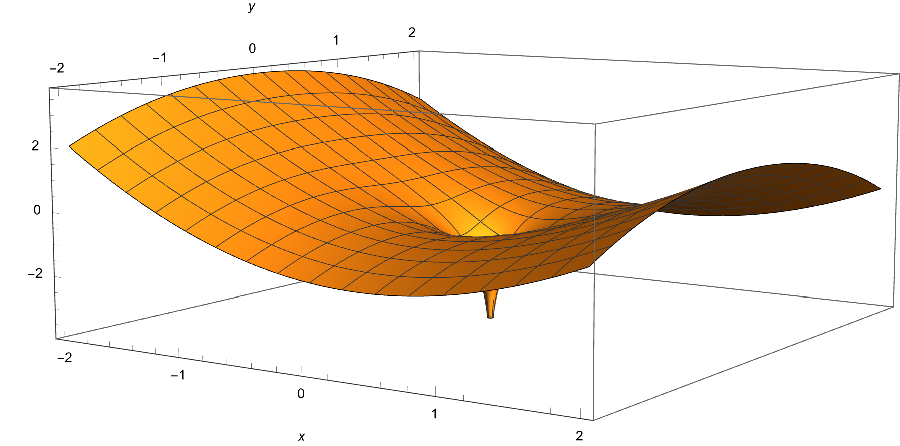
\includegraphics[height=.3\textwidth]{pictures/ReS_imaginary_3D.pdf}
	\qquad
	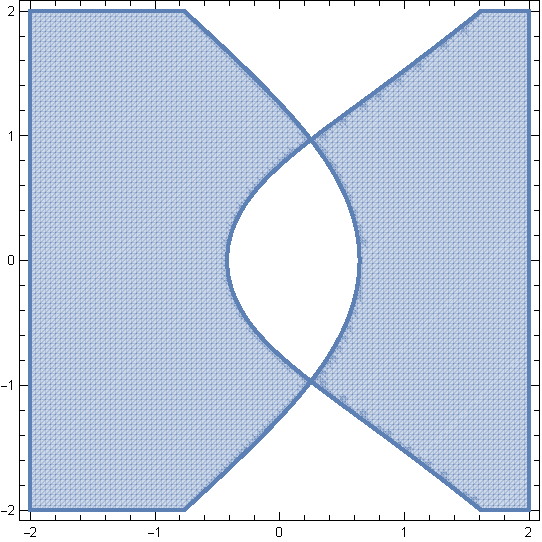
\includegraphics[height=.3\textwidth]{pictures/ReS_imaginary_region.pdf}
	\caption{A 3D plot and a region plot of the
	regions where $\operatorname{Re}S(z)-\operatorname{Re}S(z_{cr})$ is positive
	(highlighted) or negative, in the case $X=\frac{1}{2}$.
	In this case, $z_{cr}\approx 0.25+0.96 i$.}
	\label{lecture6:fig:ReS_imaginary}
\end{figure}

From the region plot, we see that the new $z$ contour should
pass through the shaded region $\operatorname{Re}S(z)-\operatorname{Re}S(z_{cr})>0$,
and the new $w$ contour should pass through the unshaded region
$\operatorname{Re}S(z)-\operatorname{Re}S(z_{cr})<0$.

Deforming the contours from \Cref{lecture6:fig:contours} to the new contours
is impossible without passing through the residue at $w=z$.
Moreover, this residue appears only for certain values of $z$. Namely,
let us first make the $z$ contour to be the positively (counterclockwise) oriented
unit circle.
It passes through the critical points $z_{cr}$ and $\overline{z_{cr}}$.
Since the original $w$ contour is to the right of the $z$ contour, we only
encounter the residue when $z$ is in the right half of the arc.

Thus, we can write
\begin{equation}
	\label{lecture6:eq:K_n_bulk_deformation}
	\oiint_{\textnormal{old contours}}=
	\oiint_{\textnormal{new contours}}
	+
	\int_{\overline{z_{cr}}}^{z_{cr}}
	2\pi i\ssp \operatorname{Res}\limits_{w=z}\ssp dz,
\end{equation}
where in the single integral, the $z$ contour passes to the right of the origin,
along the right half of the unit circle.

It remains to consider the two integrals in the right-hand side
of \eqref{lecture6:eq:K_n_bulk_deformation}.
Recall that the correlation functions are
defined relative to a reference measure, and the right object to scale is
\begin{equation*}
	K_n(x,y)dy=\frac{1}{\sqrt n}
	\ssp
	K_n(X\sqrt n+\Delta x/\sqrt n,X\sqrt n+\Delta y/\sqrt n)
	\ssp d\left( \Delta y \right).
\end{equation*}
The extra factor $n^{-1/2}$
compensates the prefactor $\sqrt n$ in
\eqref{lecture6:eq:K_n_scaling}.

The single integral takes the form
\begin{equation}
	\label{lecture6:eq:K_n_bulk_single}
	\frac{-i}{2\pi}
	\int_{\overline{z_{cr}}}^{z_{cr}}
	dz
	=\frac{\sin(\arg z_{cr})}{\pi}.
\end{equation}

The double integral
in \eqref{lecture6:eq:K_n_bulk_deformation}
has both contours
in the ``steepest descent'' regime, which means that
the main contribution is
\begin{equation*}
	\mathrm{const}\cdot
	\frac{e^{n\left( \operatorname{Re}S(z_{cr})-\operatorname{Re}S(z_{cr}) \right)}}{\sqrt n}
	\sim \frac{\mathrm{const}}{\sqrt n}.
\end{equation*}
At this rate, the double integral over the new contours
\emph{does not} contribute to the asymptotics of the correlation functions.
Recall that the correlation functions are expressed as finite-dimensional
determinants of the kernel $K_n(x,y)$, and the error $O(n^{-1/2})$ is
negligible in the limit $n\to+\infty$.
This is because the main term comes from the single integral,
which does not vanish.

Note that
\begin{equation*}
	z_{cr}=\frac{X\pm \sqrt{X^2-4}}{2},
	\qquad
	\sin(\arg z_{cr})=\frac{\sqrt{4-X^2}}{2}.
\end{equation*}
This again establishes the \emph{Wigner semicircle law} for the GUE kernel.

\begin{remark}
	This is already the third proof --- we worked with trees, the tridiagonal form,
	and now via steepest descent. The steepest descent method is the least general one,
	but it allows to access local correlations in the bulk and at the edge.
\end{remark}

We will consider other regimes, $|X|>2$ and $|X|=2$, in the next
\Cref{chap:lecture7}.





\section{Problems}

\subsection{Different global positions}
\label{lecture6:prob:different-global-positions}

Show that if in \eqref{lecture6:eq:scaling_x-y} we take $X\ne Y$, then
$K_n(x,y)$ vanishes as $n\to+\infty$. Moreover,
establish the rate of decay in $n$. Is it power-law or exponential?

\subsection{Sine kernel}
\label{lecture6:prob:sine-kernel}

Compute the integral
\eqref{lecture6:eq:K_n_bulk_single}.


\subsection{Discrete sine process}
\label{lecture6:prob:discrete-sine-process}

Define the discrete sine kernel on $\mathbb{Z}$ by
\begin{equation*}
	K_{\mathrm{dsine}}(x,y)\coloneqq
	\begin{cases}
		\dfrac{\sin \rho(x-y)}{\pi (x-y)},&\qquad x\ne y,\\[10pt]
		\dfrac{\rho}{\pi},&\qquad x=y,
	\end{cases}
\end{equation*}
where $\rho\in[0,1]$ is the density parameter.

Let $\rho=1/2$.
Compute (numerically) the asymptotics of the two events under the discrete sine process:
\begin{equation*}
	\operatorname{\mathbb{P}}
	\Bigl(
		\underbrace{\circ \circ\ldots\circ}_{n\text{ times}}
		\underbrace{\bullet \bullet\ldots\bullet}_{n\text{ times}}
	\Bigr),\qquad
	\operatorname{\mathbb{P}}
	\Bigl(
		\underbrace{\circ\bullet\circ\bullet\ldots\circ\bullet}_{2n\text{ points}}
	\Bigr),\qquad
\end{equation*}
If the sine process was of independent random points (with the same density $1/2$),
both events
would have the same probability $2^{-2n}$.
Which event is more favored by the sine process?
















\chapter{Steepest descent and local statistics. Cutting corners}
\label{chap:lecture7}





\section{Steepest descent for the GUE kernel}
\label{lecture7:sec:steepest-descent-GUE}

\subsection{Recap}

We continue the asymptotic analysis of the GUE kernel.

The GUE correlation kernel is defined by
\[
K_n(x,y)=\sum_{j=0}^{n-1}\psi_j(x)\psi_j(y),
\]
where the functions
\[
\psi_j(x)=\frac{1}{\sqrt{h_j}}\,p_j(x)\,e^{-x^2/4}
\]
are built from the monic Hermite polynomials \(p_j(x)\) with normalization constants \(h_j\) ensuring that the \(\psi_j\)'s form an orthonormal system in \(L^2(\mathbb{R})\).

Using the generating function
\[
\exp\Bigl(xt-\frac{t^2}{2}\Bigr)=\sum_{n\ge0}p_n(x)\frac{t^n}{n!},
\]
one obtains by Cauchy’s integral formula
\[
p_n(x)=\frac{n!}{2\pi i}\oint_C\frac{\exp\Bigl(xt-\frac{t^2}{2}\Bigr)}{t^{n+1}}\,dt,
\]
which leads to
\[
\psi_n(x)=\frac{e^{-x^2/4}}{\sqrt{h_n}}\frac{n!}{2\pi i}\oint_C\frac{\exp\Bigl(xt-\frac{t^2}{2}\Bigr)}{t^{n+1}}\,dt.
\]

Starting from the Fourier transform identity
\[
\int_{-\infty}^{\infty} \exp\Bigl(-\frac{t^2}{2}+i\,t\,x\Bigr)\,dt
=\sqrt{2\pi}\,e^{-x^2/2},
\]
and differentiating with respect to \(x\), then changing variables, one obtains
\[
\psi_n(x)=\frac{i\,e^{x^2/4}}{\sqrt{2\pi\,h_n}}
\int_{-i\infty}^{i\infty} s^n\,e^{s^2/2- s\,x}\,ds.
\]

By inserting the above representations for \(\psi_n(x)\) into the kernel sum, one arrives at the double contour integral formula
(after conjugation and the trick with removing $1 / (s-t)$):
\[
K_n(x,y)=\frac{1}{(2\pi)^2}
\oint_C dt\int_{-i\infty}^{i\infty}ds\,
\frac{\exp\Bigl\{\frac{s^2}{2}-sy-\frac{t^2}{2}+tx\Bigr\}}{s-t}\left(\frac{s}{t}\right)^n.
\]
The integration contour $C$ is a small contour around $0$, and
$s$ is passing to the right of $C$.

This representation is especially useful for performing asymptotic analysis (for example, via the steepest descent method) and for deriving results such as the semicircle law.


\subsection{Scaling}
\label{lecture7:sub:scaling}

Let us now consider the GUE kernel,
\begin{equation*}
	K_n(x,y)=\frac{1}{(2\pi)^2}
	\oint_C dt\int_{-i\infty}^{i\infty}ds\ssp
	\frac{\exp\left\{ \frac{s^2}{2}-sy-\frac{t^2}{2}+tx \right\}}{s-t}\left( \frac{s}{t} \right)^n
	.
\end{equation*}

We know from the Wigner semicircle law
(established for real symmetric matrices with general iid entries in
in \Cref{chap:lecture2},
and for the GUE in \Cref{chap:lecture4})
that the eigenvalues live on the scare $\sqrt n$. This means that to capture the local asymptotics,
we need to scale
\begin{equation}
	\label{lecture7:eq:scaling_x-y}
	x=X\sqrt n+\frac{\Delta x}{\sqrt n},\qquad y=Y\sqrt n+\frac{\Delta y}{\sqrt n},\qquad
	\Delta x,\Delta y\in\mathbb{R}.
\end{equation}
Moreover, if $X\ne Y$ (i.e., different global positions), one can check that the kernel
vanishes. In other words, the local behaviors at different global positions are independent.
In what follows, we take $Y=X$.


\begin{figure}[htpb]
	\centering
	\begin{tikzpicture}[scale=1]
		% Draw coordinate axes
		\draw[->] (-2,0) -- (3,0);
		\draw[->] (0,-3) -- (0,3);

		% t contour: unit circle, counterclockwise
		\draw[ultra thick,->] (1,0) arc (0:360:1);
		% Place the t label near the contour (at 45° outside the circle)
		\coordinate (TLabel) at (.5,.5);
		\node at (TLabel) {\(z\)};

		% s contour: vertical line (imaginary axis) with a detour near the origin
		% It starts at (0,-3), goes vertically to (0,-2), then detours to (0,2)
		% via a Bézier curve (pushed to the right), and finally resumes vertically to (0,3).
		\draw[ultra thick,->,red]
			(0,-3)
			-- (0,-2)
			.. controls (1.8,-2) and (1.8,2) .. node[midway, above right] {\(w\)} (0,2)
			-- (0,3);
	\end{tikzpicture}
	\caption{Integration contours for the GUE kernel.}
	\label{lecture7:fig:contours}
\end{figure}


Let us also make a change of the integration variables:
\begin{equation*}
	t=z\sqrt n,\qquad s=w\sqrt n.
\end{equation*}
The integration contours for $z$ and $w$ look the same as for $t$ and $s$, up to a rescaling
(\Cref{lecture7:fig:contours}). However, as $0$
and $t=s$
are the only singularities in the integrand, we can deform the $z,w$
contours as we wish, while keeping $|z|<|w|$
and the general shape as in \Cref{lecture7:fig:contours}.

We thus have:
\begin{multline}
	\label{lecture7:eq:K_n_scaling}
	K_n(X\sqrt n+\Delta x/\sqrt n,X\sqrt n+\Delta y/\sqrt n)\\=
	\frac{\sqrt n}{(2\pi)^2}
	\oint_C dz\int_{-i\infty}^{i\infty}dw\ssp
	\frac{\exp
		\left\{
			n\left(
				\log w -\log z
				+\frac{w^2}{2}-\frac{z^2}{2}
				+X(z-w)+\frac{z \Delta x-w \Delta y}{n}
			\right)
		\right\}
	}{w-z}.
\end{multline}
\begin{remark}
	\label{lecture7:rmk:log-harmless}
	The logarithms in the exponent are harmless, since for the
	estimates we only need the real parts of the logarithms,
	and for the main contributions, we will have $z\approx w$, so
	any phases of the logarithms would cancel.
\end{remark}

The asymptotic analysis of double contour integrals like
\eqref{lecture7:eq:K_n_scaling} in the context of determinantal point processes
was pioneered in \cite[Section~3]{Okounkov2002}.

\subsection{Critical points}
\label{lecture7:sub:critical-points}

Let us define
\begin{equation*}
	S(z)\coloneqq
	\frac{z^2}{2}+\log z -X z.
\end{equation*}
Then the exponent contains $n \left( S(w)-S(z) \right)$.
According to the steepest descent ideology, we
should deform the integration contours
to pass through the critical point(s) $z_{cr}$ of $S(z)$.
Moreover, the new $w$ contour should maximize the real part of $S(z)$
at $z_{cr}$, and the new $z$ contour should minimize it.
If $S''(z_{cr})\ne 0$, it is possible to locally choose such contours,
they will be perpendicular to each other at $z_{cr}$.

Thus, we need to find the critical points of $S(z)$.
They are found from the quadratic equation:
\begin{equation}
	\label{lecture7:eq:critical-points}
	S'(z)=z+\frac{1}{z}-X=0,\qquad
	z_{cr}=\frac{X\pm \sqrt{X^2-4}}{2}.
\end{equation}
Depending on whether $|X|<2$, there are three cases.
Unless $|X|=2$ (when equation \eqref{lecture7:eq:critical-points} has a single root), we have
$S''(z_{cr})\ne 0$.
We will consider the three cases in
\Cref{lecture7:sub:imaginary-critical-points,sub:real-critical-points,sub:double-critical-points}
below.

\subsection{Imaginary critical points: $|X|<2$, ``bulk''}
\label{lecture7:sub:imaginary-critical-points}

When $|X|<2$, the critical points are complex conjugate.
Denote them by $z_{cr}$ and $\overline{z_{cr}}$.
Since $S(z)$ has real coefficients, we have
\begin{equation*}
	\operatorname{Re}S(z_{cr})=\operatorname{Re}S(\overline{z_{cr}}).
\end{equation*}
Thus, we need to consider the contribution from both points.
For simplicity of the computations, let us consider only the case $X=0$.
See Problem~\ref{lecture7:prob:imaginary-critical-points}.
We have
\begin{equation*}
	z_{cr}=i,\qquad
	S''(z_{cr})=2.
\end{equation*}
The behavior of $\operatorname{Re}S(z)$ on the complex plane
can be illustrated by a 3D plot or by a region plot of the regions
where $\operatorname{Re}S(z)-\operatorname{Re}S(z_{cr})$ has constant sign.
See \Cref{lecture7:fig:ReS_imaginary} for an illustration in the case $X=\frac{1}{2}$.
(We take $X\ne 0$ to break symmetry, for a better intuition.)

\begin{figure}[htpb]
	\centering
	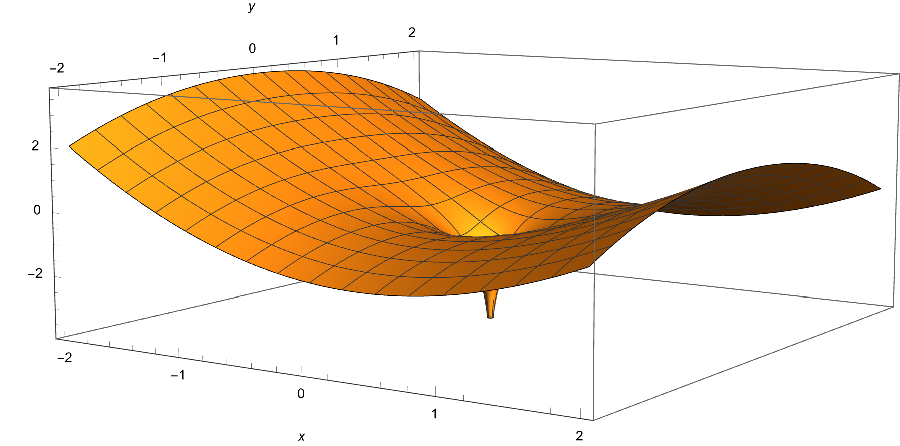
\includegraphics[height=.3\textwidth]{pictures/ReS_imaginary_3D.pdf}
	\qquad
	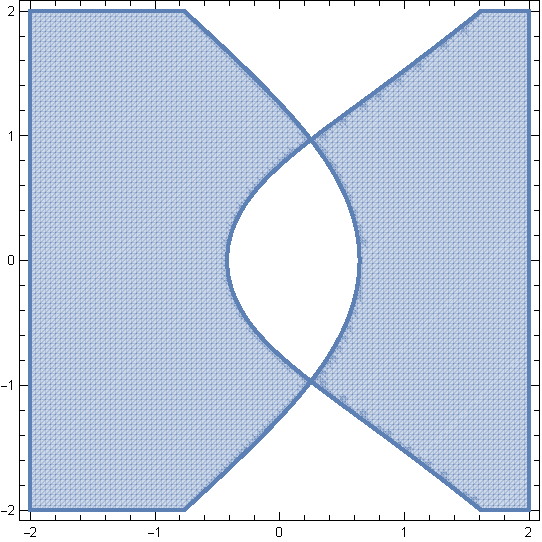
\includegraphics[height=.3\textwidth]{pictures/ReS_imaginary_region.pdf}
	\caption{A 3D plot and a region plot of the
	regions where $\operatorname{Re}S(z)-\operatorname{Re}S(z_{cr})$ is positive
	(highlighted) or negative, in the case $X=\frac{1}{2}$.
	In this case, $z_{cr}\approx 0.25+0.96 i$.}
	\label{lecture7:fig:ReS_imaginary}
\end{figure}

From the region plot, we see that the new $z$ contour should
pass through the shaded region $\operatorname{Re}S(z)-\operatorname{Re}S(z_{cr})>0$,
and the new $w$ contour should pass through the unshaded region
$\operatorname{Re}S(z)-\operatorname{Re}S(z_{cr})<0$.

Deforming the contours from \Cref{lecture7:fig:contours} to the new contours
is impossible without passing through the residue at $w=z$.
Moreover, this residue appears only for certain values of $z$. Namely, for $X=0$,
let us first make the $z$ contour to be the positively (counterclockwise) oriented
unit circle.
It passes through the critical points $z_{cr}=i$ and $\overline{z_{cr}}=-i$.
Since the original $w$ contour is to the right of the $z$ contour, we only
encounter the residue when $z$ is in the right half of the circle.

Thus, we can write
\begin{equation}
	\label{lecture7:eq:K_n_bulk_deformation}
	\oiint_{\textnormal{old contours}}=
	\oiint_{\textnormal{new contours}}
	+
	\int_{-i}^i 2\pi i\ssp \operatorname{Res}\limits_{w=z}\ssp dz,
\end{equation}
where in the single integral, the $z$ contour passes to the right of the origin,
along the right half of the unit circle.

It remains to consider the two integrals in the right-hand side
of \eqref{lecture7:eq:K_n_bulk_deformation}.
Recall that the correlation functions are
defined relative to a reference measure, and the right object to scale is
\begin{equation*}
	K_n(x,y)dy=\frac{1}{\sqrt n}\ssp d\left( \Delta y \right).
\end{equation*}
The extra factor $n^{-1/2}$
compensates the prefactor $\sqrt n$ in
\eqref{lecture7:eq:K_n_scaling}.

The single integral takes the form
\begin{equation}
	\label{lecture7:eq:K_n_bulk_single}
	\frac{-i}{2\pi}
	\int_{-i}^i
	e^{z (\Delta x -\Delta y)}
	\ssp
	dz
	=\frac{\sin\left( \Delta x-\Delta y \right)}{\pi(\Delta x-\Delta y)},
	\qquad \Delta x,\Delta y\in\mathbb{R}.
\end{equation}
\begin{definition}
	\label{lecture7:def:sine-kernel}
	The \emph{sine kernel} is defined as
	\begin{equation*}
		K_{\mathrm{sine}}(x,y)\coloneqq
		\begin{cases}
			\dfrac{\sin (x-y)}{\pi (x-y)},&\qquad x\ne 0,\\[10pt]
			\dfrac{1}{\pi},&\qquad x=0.
		\end{cases}
	\end{equation*}
	(The value at $x=y$ is defined by continuity.)

	This kernel is translation invariant, and is often
	defined with a single argument, as
	$K_{\mathrm{sine}}(x-y)$.
\end{definition}

The double integral has both contours
in the ``steepest descent'' regime, which means that
the main contribution is
\begin{equation*}
	\mathrm{const}\cdot
	\frac{e^{n\left( \operatorname{Re}S(z_{cr})-\operatorname{Re}S(z_{cr}) \right)}}{\sqrt n}
	\sim \frac{\mathrm{const}}{\sqrt n}.
\end{equation*}
At this rate, the double integral over the new contours
\emph{does not} contribute to the asymptotics of the correlation functions.
Recall that the correlation functions are expressed as finite-dimensional
determinants of the kernel $K_n(x,y)$, and the error $O(n^{-1/2})$ is
negligible in the limit $n\to+\infty$.
This is because the main term comes from the single integral,
which does not vanish.

We have established the following result:
\begin{proposition}[Bulk asymptotics at $X=0$]
	\label{lecture7:prop:bulk}
	The correlation kernel $K_n$ of the GUE has the following asymptotics
	close to zero as $n\to+\infty$:
	\begin{equation*}
		\lim_{n\to \infty}
		\frac{1}{\sqrt n}
		K_n\left( \frac{\Delta x}{\sqrt n},\frac{\Delta y}{\sqrt n} \right)
		=
		K_{\mathrm{sine}}\left( \Delta x,\Delta y \right),
		\qquad \Delta x,\Delta y\in\mathbb{R}.
	\end{equation*}
	Consequently, the eigenvalues of the GUE converge to the sine process
	determined by the sine kernel (\Cref{lecture7:def:sine-kernel}),
	in the sense of finite-dimensional distributions.
\end{proposition}

\begin{remark}
	Beyond $X=0$, the local correlations are essentially the same,
	up to rescaling of the real line by a constant factor (depending
	on the semicircle density).
	See Problem~\ref{lecture7:prob:imaginary-critical-points}.
\end{remark}

\subsection{Real critical points: $|X|>2$, ``large deviations''}
\label{lecture7:sub:real-critical-points}

For \(X^2>4\), both solutions
\eqref{lecture7:eq:critical-points}
are real. Let us assume $X>2$, the case \(X<2\) is similar.
For $X>2$, both solutions are positive.
Label these solutions as
\[
	z_+ \;=\;\frac{X + \sqrt{X^2-4}}{2},
	\qquad
	z_- \;=\;\frac{X - \sqrt{X^2-4}}{2},
	\quad
	\text{so that}\quad z_+z_-=1.
\]
A straightforward check reveals that \(z_+\!>\!1\) and \(z_-\!<\!1\) (for \(X>2\)).
Note that $S''(z)=1-z^{-2}$, which is positive for \(z_+>1\) and negative for \(z_-<1\).  Thus, the critical points \(z_+\) and \(z_-\) are a local minimum and a local maximum.
A crucial observation is that
\begin{equation*}
	S(z_+)<S(z_-).
\end{equation*}
One can deform the $z$ integration contour to pass through
$z_-$ and the $w$ contour to pass through $z_+$.
Then, on these contours, one can show that
\begin{equation*}
	\operatorname{Re}S(w)-\operatorname{Re}S(z)<0.
\end{equation*}
According to the steepest descent ideology,
we see that the main exponential behavior of the double contour integral is
\begin{equation}
	\label{lecture7:eq:Oexp}
	\exp\left\{ n\left(
		\operatorname{Re}S(z_+)-\operatorname{Re}S(z_-)
\right) \right\}=O( e^{-\delta(X)n} ), \qquad |X|>2.
\end{equation}
Here $\delta(X)>0$ for $|X|>2$, and $\delta(X)\to0$ when $|X|\to2$.

The outcome \eqref{lecture7:eq:Oexp} reflects the fact that the
Wigner semicircle law places all eigenvalues inside the
interval \(\lvert X\rvert \le 2\).
The probability to see even a single eigenvalue outside $[-2,2]$
is exponentially small.

This exponential decay corresponds to a large deviation regime.
Indeed, if at least one of the diagonal entries of the matrix
is unusually large, this corresponds to
the maximal eigenvalue to get outside the interval \([-2,2]\).
See also Problem~\ref{lecture7:prob:large-deviation}.


\subsection{Double critical point: $|X|=2$, ``edge''}
\label{lecture7:sub:double-critical-points}

Throughout the subsection, we assume that $X=2$. The case $X=-2$ is symmetric.

When \(X=2\), the two solutions in \eqref{lecture7:eq:critical-points} merge into a double critical point
$z_{cr}=1$.
We have
\[
S'(1)=0,\qquad S''(1)=0,\qquad S'''(1)=2.
\]
Thus, the usual quadratic approximation fails and one must expand to third order. Writing
\[
z=1+u,\qquad w=1+v,
\]
with \(u,v\) small, we have
\[
S(1+u)=S(1)+\frac{S'''(1)}{6}\,u^3+O(u^4)
=S(1)+\frac{u^3}{3}+O(u^4),
\]
and similarly for \(S(1+v)\). Hence, the difference in the exponents becomes
\[
S(1+v)-S(1+u)=\frac{v^3-u^3}{3}+O(u^4+v^4).
\]

To capture the correct asymptotics, we rescale the local variables by setting
\[
u=\frac{U}{n^{1/3}},\qquad v=\frac{V}{n^{1/3}},
\]
so that
\[
n\Bigl[S(1+v)-S(1+u)\Bigr]=\frac{V^3-U^3}{3}+O\Bigl(n^{-1/3}\Bigr).
\]
Moreover, the correct edge scaling for the spatial variables is obtained by writing
\[
x=2\sqrt{n}+\frac{\xi}{n^{1/6}},\qquad y=2\sqrt{n}+\frac{\eta}{n^{1/6}},\qquad \xi,\eta\in\mathbb{R}.
\]
We have
\begin{equation*}
	n\left( S(w)-S(z) \right)=n^{1/3}(\xi-\eta)+
	\frac{V^3-U^3}{3}+\xi U-\eta V+O\Bigl(n^{-1/3}\Bigr).
\end{equation*}
The terms $n^{1/3}(\xi-\eta)$ are harmless as they can be removed
by conjugation.

The region plot of $\operatorname{Re}S(z)-\operatorname{Re}S(1)$
(shown in \Cref{lecture7:fig:ReS_edge})
makes sure that we can deform the $z$ contour so that it passes through $z_{cr}=1$
as the new $U$ contour at the angles $\pm \frac{2\pi}{3}$ (where $\operatorname{Re}U^3>0$),
we can deform the $w$ contour so that it passes through $z_{cr}=1$
as the new $V$ contour at the angles $\pm \frac{\pi}{3}$ (where $\operatorname{Re}V^3<0$).
This will ensure the convergence of the new double integral.

\begin{figure}[htpb]
	\centering
	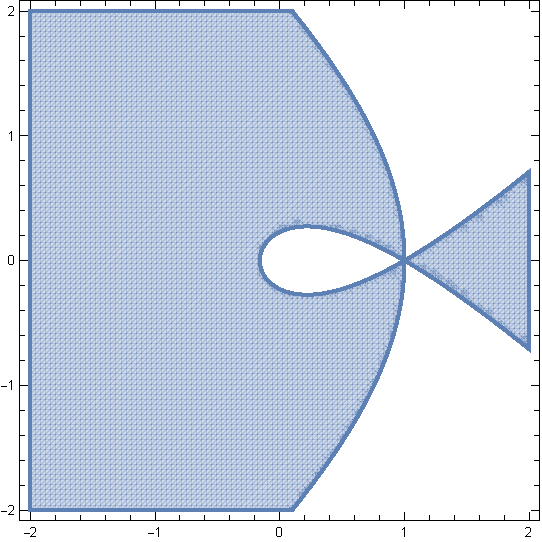
\includegraphics[height=.3\textwidth]{pictures/ReS_edge.pdf}
	\caption{The plot of the region $\operatorname{Re}S(z)-\operatorname{Re}S(1)>0$ for $X=2$.}
	\label{lecture7:fig:ReS_edge}
\end{figure}

Thus, we have shown that under the rescaling, the GUE correlation kernel
$K_n(x,y)\ssp dy$ converges to a new kernel.
\begin{definition}
	\label{lecture7:def:Airy_kernel}
	Define the \emph{Airy kernel} on $\mathbb{R}$ by
	\begin{equation*}
		K_{\mathrm{Ai}}(\xi,\eta)=\frac{1}{(2\pi i)^2}
		\int_{e^{-\frac{\pi i}{3}}\infty}^{e^{\frac{\pi i}{3}}\infty}dV
		\int_{e^{-\frac{2\pi i}{3}}\infty}^{e^{2\frac{\pi i}{3}}\infty}dU
		\ssp
		\frac{\exp\Bigl\{\frac{V^3-U^3}{3}+U\,\xi-V\,\eta\Bigr\}}{V-U}.
	\end{equation*}
	For another formula for the Airy kernel
	which does not involve integrals,
	see
	Problem~\ref{lecture7:prob:airy}.
\end{definition}

\begin{proposition}
	\label{lecture7:prop:edge}
	We have
	\begin{equation*}
		\lim_{n\to\infty}
		\frac{1}{n^{1/6}}K_n\Bigl(2\sqrt{n}+\frac{\xi}{n^{1/6}},\,2\sqrt{n}+\frac{\eta}{n^{1/6}}\Bigr)
		\to
		K_{\mathrm{Ai}}(\xi,\eta).
	\end{equation*}
	Consequently, the eigenvalue statistics at the edge of the spectrum converge to the Airy point process, in the sense of fine-dimensional distributions.
\end{proposition}

\subsection{Airy kernel, Tracy--Widom distribution, and convergence of the maximal
eigenvalue}

Let us make a few remarks on the asymptotic results of
\Cref{lecture7:prop:bulk,prop:edge}.
First,
a rigorous justification of convergence
of contour integrals requires some estimates on the error terms
in the steepest descent analysis, but these
estimates are mild and not hard to obtain.

Second, the GUE has the maximal eigenvalue $\lambda_{max}$. It is reasonable
to assume that the Airy process also (almost surely) admits a maximal point
(usually denoted by $\mathfrak{a}_1$),
and that $\lambda_{max}$
converges to $\mathfrak{a}_1$ under appropriate rescaling:
\begin{equation}
	\label{lecture7:eq:TW_GUE}
	\lim_{n\to\infty}n^{\frac{1}{6}}\bigl(\lambda_{max}-2\sqrt{n}\bigr)=\mathfrak{a}_1.
\end{equation}
This is indeed the case, but to show \eqref{lecture7:eq:TW_GUE}, one needs to
show the convergence in distribution:
\begin{equation}
	\label{lecture7:eq:TW_GUE_convergence}
	\lim_{n\to \infty}
	\mathbb{P}\Bigl(n^{1/6}(\lambda_{max}-2\sqrt{n})\le x\Bigr)
	\to
	\mathbb{P}(\mathfrak{a}_1\le x).
\end{equation}
Both events \eqref{lecture7:eq:TW_GUE_convergence} are so-called
\emph{gap probabilities}, for example,
\begin{equation*}
	\operatorname{P}(\mathfrak{a}_1\le x)=
	\operatorname{P}(\textnormal{there are no eigenvalues in the interval $(x,\infty)$}),
\end{equation*}
which is expressed as
the Fredholm determinant
\begin{equation}
	\label{lecture7:eq:gap-probability-Ai-Fredholm}
	\det\left( 1-K_{\mathrm{Ai}} \right)_{(x,\infty)}=
	1+\sum_{m=1}^{\infty}\frac{(-1)^m}{m!}
	\int_x^{\infty}dy_1\int_x^{\infty}dy_2\cdots
	\int_x^{\infty}dy_m
	\ssp
	\det\limits_{i,j=1}^m
	K_{\mathrm{Ai}}(y_i,y_j).
\end{equation}
Thus, to get \eqref{lecture7:eq:TW_GUE_convergence}), one needs to show the convergence
of sums like this for the GUE kernel
to the corresponding sums for the Airy kernel. This is doable, but tedious.

Moreover, to get convergence in distribution of random variables,
one would also have to argue either \emph{tightness},
or independently show that
\eqref{lecture7:eq:gap-probability-Ai-Fredholm} defines a
cumulative probability
distribution function in $x$:
\begin{equation}
	\label{lecture7:eq:TW_GUE_cdf}
	F_2(x)=\det\left( 1-K_{\mathrm{Ai}} \right)_{(x,\infty)}.
\end{equation}
The distribution \eqref{lecture7:eq:TW_GUE_cdf} is known as the \emph{GUE Tracy--Widom distribution}.
The subscript $2$ indicates that $\beta=2$. There are distributions
$F_\beta$ for all beta, most notably, the GOE and GSE distributions.
The classical distributions $F_1,F_2,F_4$ also appear as fluctuation distributions
in interacting particle systems, while other beta values do
not quite appear in the particle systems
domain.

More details
may be found in the original papers
\cite{tracy1993level},
\cite{Forrester1993},
\cite{tracy_widom1994level_airy}.



\subsection{Remark: what happens for general $\beta$?}

\begin{itemize}
    \item The determinantal structure exploited above is special to the $\beta=2$ case. In contrast, for $\beta=1$ (GOE) and $\beta=4$ (GSE) the eigenvalue correlations are expressed in terms of \emph{Pfaffians} rather than determinants.
			This happens before and after the scaling limit.
		\item
			Earlier attempts to extend the $\beta=2$ techniques
			were determinantal. For example, one can replace the
			squared Vandermonde $\prod_{i<j} (x_i-x_j)^2$ with
			\begin{equation*}
			 \prod_{i<j} (x_i-x_j)(x_i^{\beta/2}-x_j^{\beta/2}).
			\end{equation*}
			This is known as the \emph{Muttalib--Borodin} ensemble
			\cite{forrester2017},
			and the kernel can be computed in a similar way using (bi)orthogonalization.
		\item Local eigenvalue statistics of general $\beta$-ensembles converge to the so-called
			\emph{general $\beta$ sine process}
			and
			\emph{general $\beta$ Airy process}
			in the bulk and at the edge, respectively.
			Detailed analyses of this convergence can be found in
			\cite{RamirezRiderVirag2006RandomAiry},
			\cite{valko2009continuum},
			\cite{gorin2018stochastic},
			and the literature referenced in the recent work
			\cite{gorin2024airy}.
\end{itemize}

%%%%%%%%%%%%%%%%%%%%%%%%%%%%%%%%%%%%%%%%%%%%%%%%%%%%%%%%%%%%
\section{Cutting corners: setup}

We begin a new topic, which will be the main focus for this and the next week.

In random matrix theory, one often studies the entire spectrum of an $n\times n$ matrix ensemble such as the Gaussian Unitary Ensemble (GUE), the Gaussian Orthogonal Ensemble (GOE), or, more generally, $\beta$-ensembles. However, it is also natural to examine the spectra of \emph{principal minors} of such matrices.

When we say ``cutting corners,'' we typically refer to extracting a top-left $k\times k$ submatrix (or \emph{corner}) out of an $n\times n$ random matrix $H$ and then looking at the interplay among the eigenvalues of all corners $k=1,\dots,n$. This forms a \emph{nested} family of spectra, often described by interlacing (or Gelfand--Tsetlin) patterns.

The \emph{GUE corners process} is a classical example of
this phenomenon. If $H$ is an $n\times n$ GUE matrix, then
the top-left $k\times k$ corners (for $1\le k\le n$) have
jointly distributed eigenvalues that exhibit a
determinantal structure. We will employ the
technique of \emph{polynomial} (\emph{characteristic function}) \emph{equation} and
then \emph{loop equations} to study global limits
(note that they are not suitable to get local limits like sine and Airy processes).

So far, we have the following access to eigenvalues and corners:
\begin{enumerate}
	\item For $\beta=1,2,4$, we have the actual matrices,
		and can cut the corners in the usual way.
	\item For general $\beta$, we have the joint eigenvalue distribution
		with the interaction term $\prod_{i<j}|x_i-x_j|^\beta$, which is an interpolation.
	\item For general $\beta$, we also have the Dumitriu--Edelman
		tridiagonal model \cite{dumitriu2002matrix}.
\end{enumerate}
Cutting corners from the tridiagonal matrix is not a good idea, for many reasons.
The simplest might be that the $(n-1)\times (n-1)$ corner
eigenvalues do not have the same distribution (up to changing $n$) as the
general $\beta$ ensemble eigenvalues. Maybe we might cut the lower right corners?
Well, this is not a good idea either, because the total number of random variables
(the ``noise'') in the tridiagonal matrix is $O(n)$, while the number of eigenvalues
of all corners is $O(n^2)$.

%%%%%%%%%%%%%%%%%%%%%%%%%%%%%%%%%%%%%%%%%%%%%%%%%%%%%%%%%%%%
\section{Corners of Hermitian matrices}
\label{lecture7:sec:corners-definition}

\subsection{Principal corners}
Let $H$ be an $n\times n$ Hermitian matrix. For each $1\le k\le n$, define the \emph{top-left $k\times k$ corner} $H^{(k)}$ by
\[
	H^{(k)} \;=\; \bigl[H_{ij}\bigr]_{1\le i,j \le k}.
\]
Since $H$ is Hermitian, each $H^{(k)}$ is also Hermitian. Let
\[
	\lambda_1^{(k)} \;\ge\;\lambda_2^{(k)}\;\ge\;\cdots\;\ge\;\lambda_k^{(k)}
\]
denote the eigenvalues of $H^{(k)}$. Then the collection
\[
	\bigl\{\lambda_j^{(k)} : 1\le j\le k \le n\bigr\}
\]
is called the \emph{corners spectrum} (or \emph{minor
spectrum}) of $H$. When $H$ is random, this triangular array
of eigenvalues becomes a random point configuration in the
two-dimensional set $\{1,\dots,n\}\times \mathbb{R}$.

\subsection{Interlacing}
A fundamental feature of Hermitian matrices is that the eigenvalues of corners interlace with the eigenvalues of the full matrix:
\begin{proposition}
	\label{lecture7:prop:interlacing}
If $\nu_1\ge\dots\ge \nu_n$ are the eigenvalues of $H$ itself (i.e., the full $n\times n$ matrix), and $\mu_1\ge\cdots\ge\mu_{n-1}$ are the eigenvalues of $H^{(n-1)}$, then we have:
\[
\nu_1\;\ge\;\mu_1\;\ge\;\nu_2\;\ge\;\mu_2\;\ge\;\dots\;\ge\;\mu_{n-1}\;\ge\;\nu_n.
\]
\end{proposition}
\begin{proof}
One can prove the statement using the Courant--Fischer
(min--max) characterization of eigenvalues, often referred
to as the variational principle. Recall that for an
\(n\times n\) Hermitian matrix \(H\) with ordered
eigenvalues \(\nu_1 \ge \nu_2 \ge \cdots \ge \nu_n\), the
\(j\)-th largest eigenvalue \(\nu_j\) admits the variational
characterization
\[
\nu_j
\;=\;
\max_{\substack{V\subset\mathbb{F}^n\\\dim(V)=j}}
\;\min_{\substack{x\in V \\ x\neq 0}}
\;
\frac{x^\ast H\,x}{x^\ast x}
\;=\;
\min_{\substack{W\subset\mathbb{F}^n\\\dim(W)=n-j+1}}
\;\max_{\substack{x\in W \\ x\neq 0}}
\;
\frac{x^\ast H\,x}{x^\ast x},
\]
where \(\mathbb{F}\) is \(\mathbb{R}\), \(\mathbb{C}\), or
the quaternions (depending on \(\beta=1,2,4\),
respectively).
We leave this as Problem~\ref{lecture7:prob:interlacing}.
\end{proof}

The same interlacing property holds for real symmetric matrices ($\beta=1$),
and in the case $\beta=4$.
Therefore, it is natural to require this property for all $\beta$-ensembles.

\subsection{Orbital measure}

It is natural to consider an extended setup, and
take the matrix $H$ to not just be GUE, but instead fix its eigenvalues.
Let
\begin{equation*}
	H=U\Lambda U^\dagger,\qquad \Lambda=\operatorname{diag}(\lambda_1,\dots,\lambda_n),
\end{equation*}
where $\Lambda$ is fixed and $U\in U(n)$ is Haar (uniformly) distributed.
Denote the set of all such $H$
by $\mathrm{Orbit}(\lambda)$, $\lambda=(\lambda_1,\dots,\lambda_n)\in \mathbb{R}^n$,
$\lambda_1\ge \cdots\ge \lambda_n$.

Then, if we understand the distribution structure
of all corners of a random $H\in \mathrm{Orbit}(\lambda)$,
we can then ``average over'' the GUE eigenvalue ensemble distribution of $\lambda$
to get the GUE corners process.

\begin{remark}
	The setting with orbits presents a bridge into ``asymptotic representation theory''.
	Namely, as $n\to\infty$, how does the corners distribution look like?
	We may ask for a characterization of \emph{all the ways} how
	$\lambda^{(n)}=( \lambda_1^{(n)}\ge \ldots \lambda^{(n)}_n  )$
	goes to infinity, in such a way that the corners
	spectrum converges on all levels $k=1,\ldots,K $ for arbitrary $K$ (independent of
	$n$).
	This problem was solved in \cite{OlVer1996}.
	More direct formulas for projections of orbital measures
	were obtained in \cite{olshanski2013projections}.
\end{remark}


\section{Polynomial equation and joint distribution}

\subsection{Derivation}

Fix $\lambda=(\lambda_1\ge \ldots \ge \lambda_n )$.
Let $H\in \mathrm{Orbit}(\lambda)$ be a random matrix
(in the case $\beta=2$, but the proof works for $\beta=1,4$ as well).
Let $\mu_1,\ldots,\mu_{n-1}$ be the eigenvalues of the $(n-1)\times(n-1)$ corner $H^{(n-1)}$.
\begin{lemma}
	\label{lecture7:lemma:corner_step}
	The distribution of $\mu_1,\ldots,\mu_{n-1}$ is the same as the distribution of
	the roots of the polynomial equation
	\begin{equation}
		\label{lecture7:eq:polynomial_equation}
		\sum_{i=1}^n \frac{\xi_i}{z-\lambda_i}=0,
	\end{equation}
	where $\xi_i$ are i.i.d.\ random variables with the distribution $\chi^2_\beta$.
\end{lemma}
\begin{proof}
	$\mu_1,\ldots,\mu_{n-1} $ are the roots of the following
	equation with the determinant of
	order $n+1$:
	\begin{equation*}
		\det\begin{pmatrix}
			U\operatorname{\mathrm{diag}}(\lambda)U^\dagger-z I_N & v^\top\\
			v & 0
		\end{pmatrix}=0,
		\qquad
		v=\begin{pmatrix}
			0\\0\\\vdots\\0\\1
		\end{pmatrix}.
	\end{equation*}
	Indeed, expanding the determinant along the last row, we get the $(n-1)$th
	determinant, which corresponds to cutting the corner.

	Next, multiply the determinant by $\begin{pmatrix} U^\dagger&0\\0&1 \end{pmatrix}$
	on the left
	and $\begin{pmatrix} U & 0\\0&1 \end{pmatrix}$ on the right:
	\begin{equation*}
		\det\begin{pmatrix}
			\operatorname{\mathrm{diag}}(\lambda)-z I_N & u^\dagger\\
			u & 0
		\end{pmatrix}=0,
	\end{equation*}
	where $u^\dagger=U^\dagger v^\top$ is the last row of $U^\dagger$.
	The determinant now can be expressed as
	\begin{equation*}
		\det=-\prod_{i=1}^n(\lambda_i-z)\sum_{i=1}^{n}\frac{|u_i|^2}{\lambda_i-z}.
	\end{equation*}
	Since $u$ is a row of a Haar unitary matrix,
	it is distributed uniformly on the unit sphere in $\mathbb{C}^n$.
	However, we can identify it with a normalized vector from a
	rotationally invariant measure on $\mathbb{C}^n$,
	the best of which is Gaussian.
	This completes the proof.
\end{proof}
\begin{remark}
	\Cref{lecture7:lemma:corner_step}
	provides another proof of the eigenvalue interlacing property.
	Indeed, assume that all $\xi_i$ are rational. Then
	equation
	\eqref{lecture7:eq:polynomial_equation} is essentially $P'(z)=0$,
	where $P(z)$ is a product of powers of the $(z-\lambda_i)$'s
	(the powers depend on the $\xi_i$'s).
	As the roots of the derivative of a polynomial interlace with the roots of the polynomial,
	we get the interlacing property.
\end{remark}

\subsection{Inductive nature of the transition}

Note that when we fix $\lambda=(\lambda_1\ge \ldots \ge \lambda_n )$
and get random $\mu=(\mu_1\ge \ldots \ge \mu_{n-1} )$ by solving 
\eqref{lecture7:eq:polynomial_equation}, we can then fix $\mu$ and get random
$\nu=(\nu_1\ge \ldots \ge \nu_{n-2} )$, and so on. 
Here, $\nu$ corresponds to the $(n-2)\times(n-2)$ corner of $H$.
Indeed, we can condition on $\mu$, and conjugate $H$ again by a
unitary matrix of the form $U=\begin{pmatrix}
	U'&0\\0&1
\end{pmatrix}$, where $U'\in U(n-1)$ is Haar distributed.
Since $U\in U(n)$, this extra conjugation does not change the distribution of $H\in \mathrm{Orbit}(\lambda)$,
but it allows us to treat the passage from $\mu$ to $\nu$ on the same grounds as the 
passage from $\lambda$ to $\mu$.

\begin{remark}
	In more detail, since the homogeneous space $U(n)/U(n-1)$ 
	can be identified with $S^{2n-1}$, the $(2n-1)$-dimensional real sphere,
	we can construct a Haar-distributed unitary matrix $U\in U(n)$
	by first picking a Haar-distributed unitary matrix $U'\in U(n-1)$,
	and then picking a random point on the sphere $S^{2n-1}$.
	Restricting $H$ to $\mathbb{C}^{n-1}$ fixes the last component on the sphere 
	(up to a complex phase), but the eigenbasis of the restriction $H^{(n-1)}$
	is still Haar distributed, but now in $U(n-1)$.
\end{remark}

This implies that in order to understand the full corners process, it is enough to understand the transition from $\lambda$ to $\mu$,
where $\lambda$ is fixed, and $\mu$ is obtained by solving \eqref{lecture7:eq:polynomial_equation}.


\subsection{Case $\beta=\infty$}

In the limit $\beta\to+\infty$, the $\chi^2_\beta$ distribution
obeys the law of large numbers:
\begin{equation*}
	\frac{\chi^2_\beta}{\beta}\to 1,\qquad \beta\to+\infty.
\end{equation*}
Thus, the equation \eqref{lecture7:eq:polynomial_equation} becomes
deterministic:
\begin{equation*}
	\sum_{i=1}^n \frac{1}{z-\lambda_i}=0.
\end{equation*}
Denote 
\begin{equation}
	\label{lecture7:eq:P_z_definition}
	P(z)=\prod_{i=1}^n(z-\lambda_i).
\end{equation}
Then 
\begin{proposition}
	The passage from $\lambda=(\lambda_1\ge \ldots \ge \lambda_n )$
	to $\mu=(\mu_1\ge \ldots \ge \mu_{n-1} )$ in the limit as $\beta=\infty$
	is deterministic, and it the same as the passage from the 
	roots of the polynomial $P(z)$ \eqref{lecture7:eq:P_z_definition} to the roots of its derivative $P'(z)$.
\end{proposition}











\section{Problems}

\subsection{General bulk case}
\label{lecture7:prob:imaginary-critical-points}

Perform the asymptotic analysis of the correlation
kernel as in \Cref{lecture7:sub:imaginary-critical-points},
but in the general case $-2<X<2$.


\subsection{Large deviations}
\label{lecture7:prob:large-deviation}

Let \(W_n\) be an \(n\times n\) Wigner real or Hermitian matrix with finite variance entries. Assume that the matrix is normalized so that the variance of each diagonal entry is 1.

\medskip

\textbf{Assumption \cite{BBP2005phase}.} \textit{If a Wigner matrix is normalized to have diagonal variance 1, then a rank 1 perturbation of magnitude $c>0$ is sufficient to shoot the maximum eigenvalue outside the support of the Wigner semicircle law. (For a simulation of this phenomenon, see \href{https://lpetrov.cc/simulations/2025-01-28-bbp-transition/}{here}.)}

\medskip

Consider the following large deviation event. For a fixed \(\eta>0\), let
\[
E_{n,\eta}\coloneqq \Bigl\{ \exists\, i\in\{1,\dots,n\} \text{ such that } W_{ii}\ge \eta \Bigr\}.
\]
Under the above assumption, if for some \(i\) the diagonal
entry \(W_{ii}\) is unusually large, it will push the
maximal eigenvalue of \(W_n\) outside the bulk.

\begin{enumerate}
	\item Assuming that the
		entries are Gaussian,
		\emph{lower bound} the probability of the event \(E_{n,\eta}\) for large \(n\).
	\item
		Assuming another tail behavior of the diagonal entries (exponential or
		power-law tails),
		use the limit theorems for maxima of independent random variables to generalize the
		\emph{lower bound} of $\operatorname{\mathbb{P}}(E_{n,\eta})$.
\end{enumerate}



\subsection{Airy kernel}
\label{lecture7:prob:airy}

Define the Airy function by
\begin{equation*}
	Ai(\xi)\coloneqq
	\frac{1}{2\pi}\int_{-\infty}^\infty
	e^{i U^3/3+i\xi U} dU=
	\frac{1}{\pi}\int_0^\infty
	\cos\left( \frac{U^3}{3}+\xi U \right)\ssp dU.
\end{equation*}
This integral converges, but only conditionally. To improve convergence,
one should instead integrate
along a complex contour,
from $e^{\frac{5 \pi i}{6}}\infty$ to $0$ to
$e^{\frac{\pi i}{6}}\infty$.

Show that
\begin{equation*}
	K_{\mathrm{Ai}}(\xi,\eta)=
	\frac{Ai(\xi)\ssp Ai'(\eta)-Ai(\eta)\ssp Ai'(\xi)}{\xi-\eta}.
\end{equation*}
Note that this expression is parallel to the sine kernel,
\begin{equation*}
	\frac{\sin(x-y)}{\pi(x-y)}=\frac{\sin x\cos y-\cos x\sin y}{\pi(x-y)},\qquad
	\cos x=(\sin x)'.
\end{equation*}
These correlation kernels are called \emph{integrable}
\cite{its1990differential}.

Hint for the problem: observe that
\begin{equation*}
	\exp\left\{ -i z x+iwy \right\}=\frac{i}{x-y}\left( \frac{\partial}{\partial z}+
	\frac{\partial}{\partial w}\right)\exp\left\{ -i z x+iwy \right\},
\end{equation*}
and use integration by parts in $K_{\mathrm{Ai}}(\xi,\eta)$
from \Cref{lecture7:def:Airy_kernel}.

\subsection{Interlacing proof}
\label{lecture7:prob:interlacing}

Finish the proof of \Cref{lecture7:prop:interlacing}.















\chapter{Cutting corners and loop equations}
\label{chap:lecture8}





\section{Cutting corners: polynomial equation and distribution}

\subsection{Recap: polynomial equation}

Recall the polynomial equation we proved in the last \Cref{chap:lecture7}.
Fix $\lambda=(\lambda_1\ge \ldots \ge \lambda_n )$.
Let $H\in \mathrm{Orbit}(\lambda)$ be a random Hermitian matrix
defined as
\begin{equation*}
	H=U\ssp \mathrm{\operatorname{diag}}(\lambda_1,\ldots,\lambda_n)\ssp U^\dagger,
\end{equation*}
where $U$ is Haar-distributed unitary matrix from $U(n)$.
This is the case $\beta=2$,
but the statement holds for the cases $\beta=1,4$ with appropriate modifications.
Let $\mu_1,\ldots,\mu_{n-1}$ be the eigenvalues of the $(n-1)\times(n-1)$ corner $H^{(n-1)}$.
\begin{lemma}
	\label{lecture8:lemma:corner_step}
	The distribution of $\mu_1,\ldots,\mu_{n-1}$ is the same as the distribution of
	the roots of the polynomial equation
	\begin{equation}
		\label{lecture8:eq:polynomial_equation}
		\sum_{i=1}^n \frac{\xi_i}{z-\lambda_i}=0,
	\end{equation}
	where $\xi_i$ are i.i.d.\ random variables with the distribution $\chi^2_\beta$.
\end{lemma}
Recall also that this passage from $\lambda$ to $\mu$ works inductively, and
the distribution of the next level eigenvalues $\nu=(\nu_1\ge \ldots \ge \nu_{n-2})$
is given by the same polynomial equation, but with $\lambda$ replaced by $\mu$.
In this way, we can define a \emph{Markov map} from $\lambda$ to $\mu$, which is then iterated
to construct the full array of eigenvalues of the corners of $H$.

For $\beta=\infty$, this map is deterministic, and is equivalent to successive differentiating the
characteristic polynomial of $H$.

\subsection{Extension to general $\beta$}

We extend the polynomial equation to general $\beta$,
by \emph{declaring} (defining) that the general $\beta$ corners distribution
is powered by the passage from $\lambda=(\lambda_1\ge \ldots \ge \lambda_n)$ to $\mu=(\mu_1\ge \ldots \ge \mu_{n-1})$,
where $\mu$ solves \eqref{lecture8:eq:polynomial_equation} with $\xi_i$ i.i.d.\ $\chi^2_\beta$.
In this way, $\mu$ interlaces with $\lambda$.
For $\beta=1,2,4$, this definition reduces to the one with invariant ensembles
with fixed eigenvalues $\lambda$.


\subsection{Distribution of the eigenvalues of the corners}

Let $\mu$ be obtained from $\lambda$ by the general $\beta$ corners operation.

\begin{theorem}
	\label{lecture8:thm:corner_step}
	The density of $\mu$ with respect to the Lebesgue measure is given by
	\begin{equation*}
		\frac{\Gamma(N \beta/2)}{\Gamma(\beta/2)^n}
		\prod_{1\le i<j\le n-1}(\mu_i-\mu_j)
		\prod_{i=1}^{n-1}\prod_{j=1}^n |\mu_i-\lambda_j|^{\beta/2-1}
		\prod_{1\le i<j\le n}(\lambda_i-\lambda_j)^{1-\beta}.
	\end{equation*}
\end{theorem}
\begin{proof}
	Let $\varphi_i=\xi_i/\sum_{j=1}^n \xi_j$.
	It is well-known\footnote{See Problem~\ref{lecture8:prob:dirichlet}.}
	the joint
	density of $(\varphi_1,\ldots,\varphi_n )$ is the
	(symmetric) Dirichlet density
	\begin{equation*}
		\frac{\Gamma(N \beta/2)}{\Gamma(\beta/2)^n}
		\ssp
		w_1^{\beta/2-1}\ldots  w_n^{\beta/2-1}
		\ssp
		dw_1\ldots dw_{n-1}
	\end{equation*}
	(note that the density is $(n-1)$-dimensional).

	We need to compute the Jacobian of the transformation from $\varphi$ to $\mu$,
	if we write
	\begin{equation*}
		\sum_{i=1}^n\frac{\varphi_i}{z-\lambda_i}=
		\frac{\prod_{i=1}^{n-1}(z-\mu_i)}
		{\prod_{i=1}^n(z-\lambda_i)},
	\end{equation*}
	and compute
	(as a decomposition into partial fractions):
	\begin{equation*}
		\varphi_a=
		\frac{\prod_{i=1}^{n-1}(\lambda_a-\mu_i)}{\prod_{i\ne a}(\lambda_a-\lambda_i)}.
	\end{equation*}
	Therefore,
	\begin{equation}
		\label{lecture8:eq:Jacobian}
		\frac{\partial\varphi_a}{\partial\mu_b}=
		\frac{\prod_{i=1}^{n-1}(\lambda_a-\mu_i)}{\prod_{i\ne a}(\lambda_a-\lambda_i)}
		\ssp\frac{1}{\mu_b-\lambda_a},
		\qquad
		a=1,\ldots,n,\quad b=1,\ldots,n-1.
	\end{equation}
	The Jacobian is essentially the determinant of the matrix $1/(\mu_b-\lambda_a)$,
	which is the Cauchy determinant
	(Problems~\ref{lecture8:prob:cauchy} and~\ref{lecture8:prob:n_n_1}).
	The final density is obtained from the symmetric Dirichlet density,
	but we plug in $w=\varphi$, and also multiply by the inverse of the Jacobian determinant~\eqref{lecture8:eq:Jacobian}.
	After the necessary simplifications, this completes the proof.
\end{proof}



\begin{corollary}[Joint density of the corners]
	\label{lecture8:cor:corners_density}
	The eigenvalues $\lambda^(k)_j$, $1\le j\le k\le n$,
	of a random matrix from $\mathrm{Orbit}(\lambda)$
	form an interlacing array, with the joint density
	\begin{equation*}
		\propto
		\prod_{k=1}^n
		\prod_{1\le i<j\le k}\left(\lambda_j^{(k)}-\lambda_i^{(k)}\right)^{2-\beta}
		\prod_{a=1}^{k+1}\prod_{b=1}^k
		\left|\lambda_a^{(k+1)}-\lambda_b^{(k)}\right|^{\beta/2-1}.
	\end{equation*}
\end{corollary}
For $\beta=2$, all factors disappear, and we get the
uniform distribution on the interlacing array. This is the \emph{uniform Gibbs property}
which is important for other models, including discrete ensembles.


\section{Loop equations}

Let us write down the \emph{loop equations} for the passage from the
eigenvalues $\lambda$ to the eigenvalues $\mu$.
These loop equations are due to \cite{gorin2022dynamical}
by a limit from a discrete system (related to Jack
symmetric polynomials). Note that despite the name, these are not \textbf{equations},
but rather a statement that some expectations are holomorphic.
We stick to the random matrix setting, and
present a formulation and a proof given by \cite{gorin2025private}.

\subsection{Formulation}

\begin{theorem}
	\label{lecture8:Theorem_loop_equation}
 We fix $n=1,2,\dots$ and $n+1$ real numbers $\lambda_1\ge\dots\ge\lambda_{n+1}$. For $\beta>0$, consider $n+1$ i.i.d.\ $\chi^2_\beta$ random variables $\xi_i$ and set
 $$
  w_i=\frac{\xi_i}{\sum_{j=1}^{n+1} \xi_j}, \qquad 1\le i \le n+1.
 $$
 We define $n$ random points $\{\mu_1,\dots,\mu_n\}$ as $n$ solutions to the equation
 \begin{equation} \label{lecture8:eq_mu_equation}
  \sum_{i=1}^{n+1} \frac{w_i}{z-\lambda_i}=0.
 \end{equation}
 Take any \emph{polynomial} $W(z)$ and consider the complex function:
 \begin{equation}
 \label{lecture8:eq_loop_observable}
 f_W(z)=\operatorname{\mathbb{E}}\left[\prod_{j=1}^n \exp\bigl(W(\mu_j)\bigr) \frac{\prod_{i=1}^{n+1} (z-\lambda_i)}{\prod_{j=1}^n (z-\mu_j)} \left( W'(z)+\sum_{i=1}^{n+1} \frac{\beta/2-1}{z-\lambda_i} + \sum_{j=1}^n \frac{1}{z-\mu_j}\right)\right].
 \end{equation}
 Then $f_W(z)$ is an \emph{entire function} of $z$, in the following sense:
 \begin{itemize}
	 \item For $z\in \mathbb{C}\setminus [\lambda_{n+1},\lambda_1]$, the expectation in \eqref{lecture8:eq_loop_observable} defines a holomorphic function of $z$.
  \item This function has an analytic continuation to $\mathbb{C}$, which has no singularities.
 \end{itemize}
\end{theorem}
\begin{remark}
 Note that for $z$ in
 $[\lambda_{n+1},\lambda_1]$, the integral determining
 \eqref{lecture8:eq_loop_observable} might be divergent, and,
 therefore, analytic continuation is the proper way to
 define $f_W(z)$, $z\in [\lambda_{n+1},\lambda_1]$.
\end{remark}

\begin{corollary}
	We have
\begin{equation*}
	f_0(z)=\frac{(n+1)\beta}{2}-1.
\end{equation*}
Here $f_0$ means $f_W$ with $W\equiv 0$.
\end{corollary}
\begin{proof}
This is obtained by sending $z\to \infty$ in
	\eqref{lecture8:eq_loop_observable}.
\end{proof}

\subsection{Proof of \Cref{lecture8:Theorem_loop_equation} for $\beta>2$}

\Cref{lecture8:Theorem_loop_equation} remains
valid for $\beta>0$, but we only prove it for $\beta>2$ here.
We also assume that $\lambda_1>\ldots>\lambda_n $.


We begin by observing that for $z \in \mathbb{C} \setminus [\lambda_{n+1}, \lambda_1]$, the expectation in \eqref{lecture8:eq_loop_observable} is well-defined and holomorphic in $z$. This follows since for such $z$, the denominators $z-\lambda_i$ and $z-\mu_j$ are bounded away from zero with probability 1.
The key challenge is to show that $f_W(z)$ can be analytically continued to an entire function.
Potential singularities of $f_W(z)$ are inside the intervals $(\lambda_{i+1}, \lambda_{1})$. We will show that these singularities do not actually occur.

Consider a specific interval $(\lambda_2, \lambda_{1})$. We need to show that $f_W(z)$ has no singularities in this interval.
From \Cref{lecture8:thm:corner_step}, the probability distribution of $\mu = (\mu_1, \ldots, \mu_n)$ has density proportional to:
\begin{equation*}
	\prod_{1\le i<j\le n} (\mu_i - \mu_j) \prod_{i=1}^{n} \prod_{j=1}^{n+1} |\mu_i - \lambda_j|^{\beta/2-1}.
\end{equation*}

Let us analyze the function in \eqref{lecture8:eq_loop_observable}. For $z \in (\lambda_2, \lambda_{1})$, we need to demonstrate that the expectation
\begin{equation*}
	\operatorname{\mathbb{E}}\left[\prod_{j=1}^n \exp\bigl(W(\mu_j)\bigr) \frac{\prod_{i=1}^{n+1} (z-\lambda_i)}{\prod_{j=1}^n (z-\mu_j)} \left( W'(z)+\sum_{i=1}^{n+1} \frac{\beta/2-1}{z-\lambda_i} + \sum_{j=1}^n \frac{1}{z-\mu_j}\right)\right]
\end{equation*}
is holomorphic.
This expectation is an $(n-1)$-fold integral over $\mu_1, \ldots, \mu_n$.
For $z\in(\lambda_2,\lambda_1)$, we will show that
the one-dimensional integral over $\mu_1$ is already holomorphic,
and the remaining integrals are over domains which do not encounter singularities in $z$. We
need to consider the integral
\begin{equation}
\label{lecture8:eq:integral_original}
\begin{split}
	&\int\limits_{\lambda_2}^{\lambda_1}
	\prod_{1 \leq i<j \leq n}(\mu_i-\mu_j) \prod_{j=1}^{n}\prod_{i=1}^{n+1}(\mu_j-\lambda_i)^{\beta/2-1} \prod_{j=1}^{n} e^{W(\mu_j)} \frac{\prod_{i=1}^{n+1}(z-\lambda_i)}{\prod_{j=1}^{n}(z-\mu_j)} \\
	&\hspace{150pt}\times
	\left(W'(z) + \sum_{i=1}^{n+1} \frac{\beta/2-1}{z-\lambda_i} + \sum_{j=1}^{n} \frac{1}{z-\mu_j}\right) d\mu_2.
\end{split}
\end{equation}
Note that (here we are using the fact that $\beta>2$)
\begin{multline*}
	0 = \int_{\lambda_2}^{\lambda_1}d\mu_1
	\frac{\partial}{\partial
	\mu_1}\left(\underbrace{\prod_{1 \leq i<j \leq n}(\mu_i-\mu_j)
	\prod_{j=1}^{n}\prod_{i=1}^{n+1}(\mu_j-\lambda_i)^{\beta/2-1} \prod_{j=1}^{n} e^{W(\mu_j)}
	\frac{\prod_{i=1}^{n+1}(z-\lambda_i)}{\prod_{j=1}^{n}(z-\mu_j)}}_{(*)}\right)
	\\
	=
	\int_{\lambda_2}^{\lambda_1}d\mu_1\ssp
	(*)
	\cdot \left[\sum_{j=2}^n \frac{1}{\mu_1-\mu_j} +
	\sum_{i=1}^{n+1} \frac{\beta/2-1}{\mu_1-\lambda_i} +
	W'(\mu_1) + \frac{1}{z-\mu_1}\right].
\end{multline*}

Subtracting this expression from our original integral
\eqref{lecture8:eq:integral_original}
and noting that
\begin{equation*}
\left(W'(z) + \sum_{i=1}^{n+1} \frac{\beta/2-1}{z-\lambda_i} + \sum_{j=1}^{n} \frac{1}{z-\mu_j}\right) - \left(\sum_{j=2}^n \frac{1}{\mu_1-\mu_j} + \sum_{i=1}^{n+1} \frac{\beta/2-1}{\mu_1-\lambda_i} + W'(\mu_1) + \frac{1}{z-\mu_1}\right)
\end{equation*}
has zero at $z = \mu_1$, we conclude that our integral has no singularity at $\mu_1$, and therefore no singularities in the $[\lambda_2, \lambda_1]$ interval.
This completes the proof of \Cref{lecture8:Theorem_loop_equation} for $\beta>2$.


\section{Applications of loop equations}

The loop equations provide a powerful tool for analyzing the spectral properties of random matrices through their eigenvalue distributions. Let us derive an equation for the Stieltjes transform of the empirical measures.

\subsection{Stieltjes transform equations}
Starting from Theorem \ref{lecture8:Theorem_loop_equation} with $W=0$, we have:
\begin{equation} \label{lecture8:eq:loop_eq_base}
	\operatorname{\mathbb{E}}\left[\frac{\prod_{i=1}^{n+1}(z-\lambda_i)}{\prod_{j=1}^n(z-\mu_j)}\left(\sum_{i=1}^{n+1}\frac{\beta/2-1}{z-\lambda_i} + \sum_{j=1}^n\frac{1}{z-\mu_j}\right)\right] = \frac{(n+1)\beta}{2}-1.
\end{equation}
Let us introduce the empirical Stieltjes transforms:
\begin{align*}
G_\lambda(z) &= \frac{1}{n}\sum_{i=1}^{n+1}\frac{1}{z-\lambda_i}, \\
G_\mu(z) &= \frac{1}{n}\sum_{j=1}^n\frac{1}{z-\mu_j}.
\end{align*}
We also define the ``logarithmic potentials'' (indefinite integrals of the Stieltjes transforms):
\begin{align*}
\int G_\lambda(z)dz &= \frac{1}{n}\sum_{i=1}^{n+1}\ln(z-\lambda_i), \\
\int G_\mu(z)dz &= \frac{1}{n}\sum_{j=1}^n\ln(z-\mu_j).
\end{align*}
We understand the integrals up to the same integration constant (and branch), so the exponent of the difference
yields the original product:
\begin{equation*}
	\frac{\prod_{i=1}^{n+1}(z-\lambda_i)}{\prod_{j=1}^n(z-\mu_j)} = \exp\left(n\left(\int G_\lambda(z) - \int G_\mu(z)\right)\right)
\end{equation*}
We can rewrite equation \eqref{lecture8:eq:loop_eq_base} as:
\begin{equation} \label{lecture8:eq:stieltjes_transform_eq}
	\operatorname{\mathbb{E}}\left[\exp\left(n\left(\int G_\lambda(z)\,dz - \int G_\mu(z)\,dz\right)\right)\left(\left(\frac{\beta}{2}-1\right)G_\lambda(z) + G_\mu(z)\right)\right] = \frac{\beta}{2} + \frac{1}{n}\left(\frac{\beta}{2}-1\right).
\end{equation}





\subsection{Asymptotic behavior}

Equation \eqref{lecture8:eq:stieltjes_transform_eq} can be reinterpreted in terms of a time evolution of eigenvalue distributions. This perspective offers significant insights into the asymptotic behavior of the corners process.

If we think of $\lambda$ as configuration at time $t=1$ and $\mu$ as configuration at time $t=1-\frac{1}{n}$, then denoting the general time parameter as $t$ and setting $G_\lambda = G_1$, $G_\mu = G_{1-\frac{1}{n}}$, we obtain a continuous time evolution of Stieltjes transforms.
(And similarly for all $t$, of course.)

As $n \to \infty$, equation \eqref{lecture8:eq:stieltjes_transform_eq} transforms into:
\begin{equation*}
\frac{\beta}{2} \exp\left(\frac{\partial}{\partial t}\int G_t(z)\,dz\right) \cdot G_t(z) = \frac{\beta}{2}.
\end{equation*}
This implies
\begin{equation*}
\frac{\partial}{\partial t}\int G_t(z)\,dz + \ln G_t(z) = 0.
\end{equation*}
Taking the derivative with respect to $z$, we get:
\begin{equation}
\label{lecture8:eq:burgers_equation}
\frac{\partial}{\partial t}G_t(z) + \frac{1}{G_t(z)}\frac{\partial}{\partial z}G_t(z) = 0.
\end{equation}

This is the inviscid Burgers equation, a
fundamental nonlinear PDE in fluid dynamics --- but with complex $z$.
The complex Burgers equation has appeared in descriptions of
limit shapes of models in statistical mechanics, such as lozenge tilings
\cite{OkounkovKenyon2007Limit}.

\begin{remark}
	We see that the Burgers equation \eqref{lecture8:eq:burgers_equation} does not depend on $\beta$,
	which is expected. Indeed, for example, G$\beta$E eigenvalues
	have the same Wigner semicircle law as $\beta=2$, up to an overall
	rescaling.
\end{remark}

\subsection{Example: G$\beta$E and the semicircle law}

The Stieltjes transform of the semicircular law is given by:
\begin{equation*}
	G(z) = \int\limits_{-2}^{2}\frac{1}{z-x}\frac{\sqrt{4-x^2}}{2\pi}dx =
	\frac{1}{2} \left(z-\sqrt{z^2-4}\right).
\end{equation*}
We take this as the function $G_t(z)$ for $t=1$.
Then, for each $0\le t\le 1$, the 
G$\beta$E solution should be 
\begin{equation*}
	\frac{1}{n}\sum_{i=1}^{\lfloor nt \rfloor }\frac{1}{z-\lambda_i^{(\lfloor nt \rfloor )}}
	\to t\ssp G^{(\sqrt t)}(z),
\end{equation*}
where 
\begin{equation*}
	G^{(c)}(z) \coloneqq \frac{z-\sqrt{z^2-4c^2}}{2c^2},
\end{equation*}
is the Stieltjes transform of the semicircular law on $[-2c, 2c]$.

\begin{lemma}
	\label{lecture8:lemma:semicircle_and_burgers}
	The function $G_t(z)\coloneqq t\ssp G^{(\sqrt t)}(z)$
	satisfies the Burgers equation \eqref{lecture8:eq:burgers_equation}.
\end{lemma}
\begin{proof}
	Straightforward verification.
\end{proof}
















\section{Problems}


\subsection{Cauchy determinant}
\label{lecture8:prob:cauchy}

Prove the Cauchy determinant formula:
\begin{equation*}
	\det\left( \frac{1}{x_i-y_j} \right)_{1\le i,j\le n}=
	\frac{\prod_{i<j}(x_i-x_j)(y_i-y_j)}{\prod_{i,j}(x_i-y_j)}.
\end{equation*}

\subsection{Jacobian from $n-1$ to $n$ dependent variables}
\label{lecture8:prob:n_n_1}

Explain how the factor $\prod_{i=1}^{n-1}\prod_{j=1}^n|\mu_i-\lambda_j|$
appears from the Jacobian of the transformation from $\varphi$ to $\mu$
\eqref{lecture8:eq:Jacobian},
even though $\partial\varphi_a/\partial\mu_b$ is defined for
$a=1,\ldots,n  $, $b=1,\ldots,n-1$,
but the $\varphi_i$'s are not independent.

\subsection{Dirichlet density}
\label{lecture8:prob:dirichlet}

Find in the literature or prove on your own
the first statement in the proof of
\Cref{lecture8:thm:corner_step} about the symmetric Dirichlet density arising from
normalizing the $\xi_i$'s to $\varphi_i$'s.

\subsection{General beta Gaussian density and cutting corners}

Show that if $\lambda_1,\ldots,\lambda_{n+1} $ have the Gaussian beta density of order $n+1$,
\begin{equation*}
	\propto \prod_{1\le i<j\le n+1}(\lambda_i-\lambda_j)^{\beta} \prod_{i=1}^{n+1}e^{-\beta\lambda_i^2/2},
\end{equation*}
and $\mu_1,\ldots,\mu_n $ are obtained from $\lambda_1,\ldots,\lambda_{n+1}$
by cutting the corner (so have the conditional density as in \Cref{lecture8:thm:corner_step}),
then $\mu_1,\ldots,\mu_n$ have the Gaussian beta density of order $n$.

\subsection{General $\beta$ Corners Process Simulation}
\label{lecture8:prob:corners_simulation}

This problem explores computational aspects of the general $\beta$ corners process.

\begin{enumerate}[(a)]
\item Write code for generating a sample from the distribution of $\mu = (\mu_1, \ldots, \mu_{n-1})$ given $\lambda = (\lambda_1, \ldots, \lambda_n)$ for arbitrary $\beta > 0$, using the polynomial equation characterization.

\item Let $\lambda = (n, n-1, \ldots, 2, 1)$. For $n = 7$, compute (numerically) the expected values $\mathbb{E}[\mu_i]$ for each $i$, when $\beta = 1, 2, 4,$ and $10$. Describe the behavior as $\beta$ increases.
\end{enumerate}














\chapter{Loop equations and asymptotics to Gaussian Free Field}
\label{chap:lecture9}




\section{Recap}

\subsection{(Dynamical) loop equations}

\begin{theorem}
	\label{lecture9:Theorem_loop_equation}
 We fix $n=1,2,\dots$ and $n+1$ real numbers $\lambda_1\ge\dots\ge\lambda_{n+1}$. For $\beta>0$, consider $n+1$ i.i.d.\ $\chi^2_\beta$ random variables $\xi_i$ and set
 $$
  w_i=\frac{\xi_i}{\sum_{j=1}^{n+1} \xi_j}, \qquad 1\le i \le n+1.
 $$
 We define $n$ random points $\{\mu_1,\dots,\mu_n\}$ as $n$ solutions to the equation
 \begin{equation} \label{lecture9:eq_mu_equation}
  \sum_{i=1}^{n+1} \frac{w_i}{z-\lambda_i}=0.
 \end{equation}
 Take any \emph{polynomial} $W(z)$ and consider the complex function:
 \begin{equation}
 \label{lecture9:eq_loop_observable}
 f_W(z)=\operatorname{\mathbb{E}}\left[\prod_{j=1}^n \exp\bigl(W(\mu_j)\bigr) \frac{\prod_{i=1}^{n+1} (z-\lambda_i)}{\prod_{j=1}^n (z-\mu_j)} \left( W'(z)+\sum_{i=1}^{n+1} \frac{\beta/2-1}{z-\lambda_i} + \sum_{j=1}^n \frac{1}{z-\mu_j}\right)\right].
 \end{equation}
 Then $f_W(z)$ is an \emph{entire function} of $z$, in the following sense:
 \begin{itemize}
	 \item For $z\in \mathbb{C}\setminus [\lambda_{n+1},\lambda_1]$, the expectation in \eqref{lecture9:eq_loop_observable} defines a holomorphic function of $z$.
  \item This function has an analytic continuation to $\mathbb{C}$, which has no singularities.
 \end{itemize}
\end{theorem}

We proved this statement for $\beta>2$, but it is valid for all $\beta>0$.

\subsection{Loop equations for $W=0$}

When $W=0$, the loop equation \eqref{lecture9:eq_loop_observable} becomes
\begin{equation*}
	f_0(z)=\frac{(n+1)\beta}{2}-1,
\end{equation*}
so
\begin{equation*}
		\operatorname{\mathbb{E}}\left[\frac{\prod_{i=1}^{n+1}(z-\lambda_i)}{\prod_{j=1}^n(z-\mu_j)}\left(\sum_{i=1}^{n+1}\frac{\beta/2-1}{z-\lambda_i} + \sum_{j=1}^n\frac{1}{z-\mu_j}\right)\right] = \frac{(n+1)\beta}{2}-1.
\end{equation*}

Recall that we defined
\begin{align*}
G_\lambda(z) = \frac{1}{n}\sum_{i=1}^{n+1}\frac{1}{z-\lambda_i},
\qquad
G_\mu(z) = \frac{1}{n}\sum_{j=1}^n\frac{1}{z-\mu_j}.
\end{align*}
We also define the ``logarithmic potentials'' (indefinite integrals of the Stieltjes transforms):
\begin{align*}
\int G_\lambda(z)dz = \frac{1}{n}\sum_{i=1}^{n+1}\ln(z-\lambda_i), \qquad
\int G_\mu(z)dz = \frac{1}{n}\sum_{j=1}^n\ln(z-\mu_j).
\end{align*}
We understand the integrals up to the same integration constant (and branch), so the exponent of the difference
yields the original product:
\begin{equation*}
	\frac{\prod_{i=1}^{n+1}(z-\lambda_i)}{\prod_{j=1}^n(z-\mu_j)} = \exp\left(n\left(\int G_\lambda(z) - \int G_\mu(z)\right)\right)
\end{equation*}
We can rewrite
the loop equation
as:
\begin{equation} \label{lecture9:eq:stieltjes_transform_eq}
	\operatorname{\mathbb{E}}\left[\exp\left(n\left(\int G_\lambda(z)\,dz - \int G_\mu(z)\,dz\right)\right)\left(\left(\frac{\beta}{2}-1\right)G_\lambda(z) + G_\mu(z)\right)\right] = \frac{\beta}{2} + \frac{1}{n}\left(\frac{\beta}{2}-1\right).
\end{equation}

\subsection{The full corners process}

Assume $n$ is going to infinity, and we fix a sequence of
top-level eigenvalues $\lambda^{(n)}_j$, $1\le j \le n$,
growing in some way. This sequence can be random
(like G$\beta$E rescaled to have eigenvalues in a bounded interval)
or deterministic
(for example, $\lambda^{(n)}$ has $n/10$ points at $0$,
$n/10$ points at $1$, and $8n/10$ points at $2$,
see \Cref{lecture9:fig:corners}).
\begin{figure}[htpb]
	\centering
	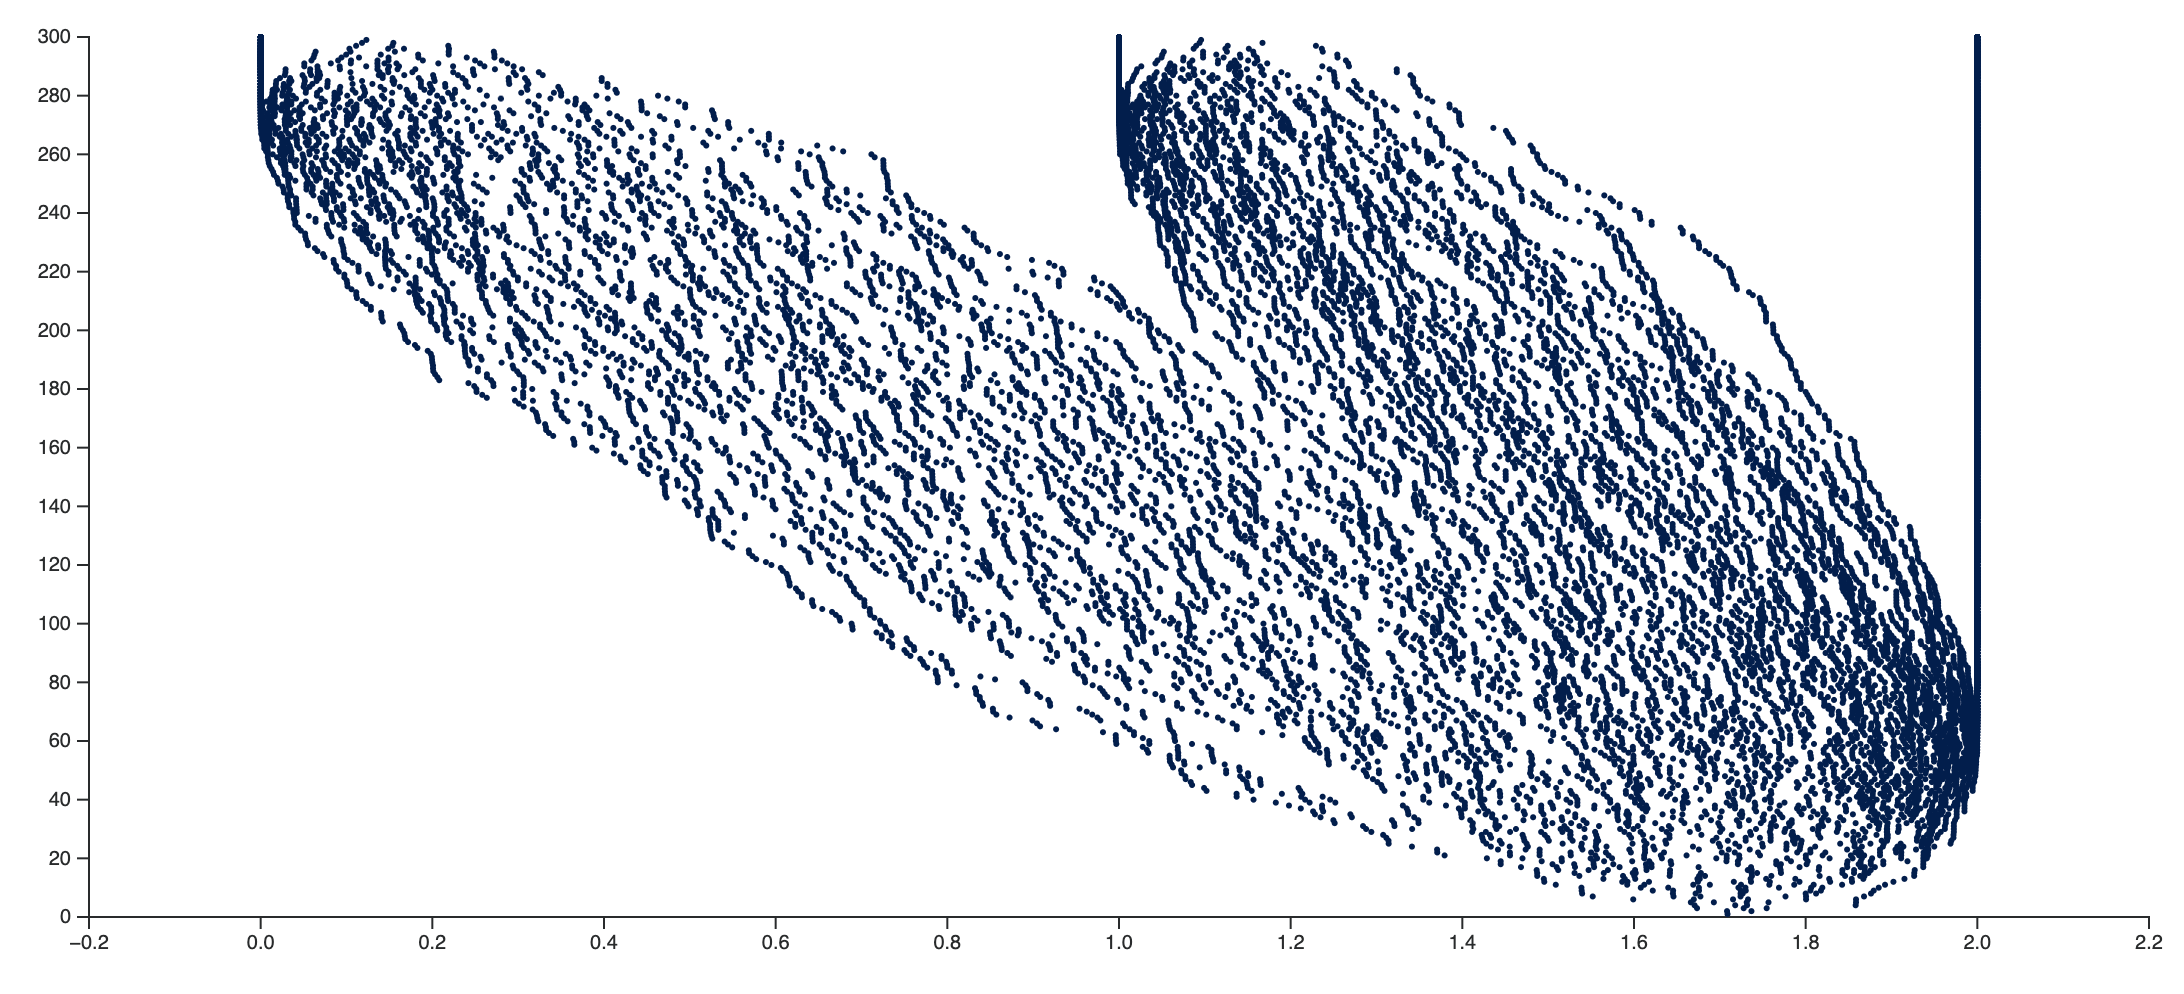
\includegraphics[width=\textwidth]{./pictures/corners.png}
	\caption{Corners process for $n=300$,
	$\beta=1$, with $n/10$ points at $0$,
	$n/10$ points at $1$, and $8n/10$ points at $2$ on the top level.}
	\label{lecture9:fig:corners}
\end{figure}

Denote the eigenvalues
of the $k\times k$ beta corner (that is,
obtained by successively solving the polynomial equation
\eqref{lecture9:eq_mu_equation}
$n-k$ times) by $\lambda^{(k)}_j$, $1\le j \le k$.
As $n\to\infty$, we postulate that
\begin{quote}
	The empirical distribution of $\lambda^{(k)}_j$
	converges to some deterministic probability measure
	$\mathfrak{m}_t$, where $k/n\to t\in[0,1]$.
	Consequently, the Stieltjes transform $G_{\lambda^{(k)}}(z)$
	converges to $G_t(z)$, for $z$ in a complex domain
	outside of the support of $\mathfrak{m}_t$.
\end{quote}
Note that we do not assume the scaling of the
$\lambda^{(k)}_j$'s, for convenience.

Denote by $\displaystyle
G_t(z)=\int_{\mathbb{R}}\frac{\mathfrak{m}_t(dx)}{z-x}$
the Stieltjes transform of the measure $\mathfrak{m}_t$.

\begin{proposition}
	The functions $G_t(z)$ satisfy the complex Burgers equation
	\begin{equation*}
		\frac{\partial}{\partial t}G_t(z) +
		\frac{1}{G_t(z)}\frac{\partial}{\partial z}G_t(z) = 0.
	\end{equation*}
\end{proposition}
\begin{proof}
	We have in \eqref{lecture9:eq:stieltjes_transform_eq},
	if $\lambda$ and $\mu$ live on levels $t$ and $t-\frac{1}{n}$,
	respectively:
	\begin{equation*}
		G_\lambda(z)-G_\mu(z)\approx
		\frac{1}{n}\ssp\frac{\partial}{\partial t}G_t(z),
		\qquad
		\left( \frac{\beta}{2}-1 \right)G_\lambda(z) + G_\mu(z) \approx
		\frac{\beta}{2}\ssp G_t(z) - \frac{1}{n}\ssp\frac{\partial}{\partial t}G_t(z)
		\approx
		\frac{\beta}{2}\ssp G_t(z) .
	\end{equation*}
	Due to the concentration assumption, we can ignore the expectation.
	Then, taking the logarithm of \eqref{lecture9:eq:stieltjes_transform_eq},
	and differentiating with respect to $z$,
	we get the Burgers equation.
\end{proof}

\subsection{Example: G$\beta$E and the semicircle law}

The Stieltjes transform of the semicircular law is given by:
\begin{equation*}
	G(z) = \int\limits_{-2}^{2}\frac{1}{z-x}\frac{\sqrt{4-x^2}}{2\pi}dx =
	\frac{1}{2} \left(z-\sqrt{z^2-4}\right).
\end{equation*}
We take this as the function $G_t(z)$ for $t=1$.
Then, for each $0\le t\le 1$, the
G$\beta$E solution should be
\begin{equation*}
	\frac{1}{n}\sum_{i=1}^{\lfloor nt \rfloor }\frac{1}{z-\lambda_i^{(\lfloor nt \rfloor )}}
	\to t\ssp G^{(\sqrt t)}(z),
\end{equation*}
where
\begin{equation*}
	G^{(c)}(z) \coloneqq \frac{z-\sqrt{z^2-4c^2}}{2c^2},
\end{equation*}
is the Stieltjes transform of the semicircular law on $[-2c, 2c]$.

\begin{lemma}
	\label{lecture9:lemma:semicircle_and_burgers}
	The function $G_t(z)\coloneqq t\ssp G^{(\sqrt t)}(z)$
	satisfies the Burgers equation.
\end{lemma}
\begin{proof}
	Straightforward verification.
\end{proof}



\section{Gaussian Free Field}
\label{lecture9:sec:GFF}

The \emph{Gaussian Free Field} (GFF) is a fundamental object in probability theory and mathematical physics. Roughly speaking, it can be viewed as a multi-dimensional analog of Brownian motion: instead of one-dimensional “time,” the underlying parameter space is a multi-dimensional domain (often two-dimensional). In one dimension, the GFF reduces to an ordinary Brownian bridge (or motion). In higher dimensions, it becomes a random generalized function (a “distribution”) whose covariance structure is governed by the appropriate Green's function of the Laplacian. Below we provide an introduction, starting from finite-dimensional Gaussian vectors and culminating in the GFF as a random distribution.

\subsection{Gaussian correlated vectors and random fields}
\label{lecture9:subsec:gauss_vectors_random_fields}

Recall that an $n$-dimensional real-valued random vector $X = (X_1,\dots, X_n)$ is called \emph{Gaussian} if every linear combination
\[
\alpha_1 X_1 + \cdots + \alpha_n X_n
\]
of its components is a univariate Gaussian random variable. The law of such a vector is completely determined by its mean vector $m \in \mathbb{R}^n$ and its covariance matrix $\Sigma \in \mathbb{R}^{n\times n}$. The density function, for invertible $\Sigma$, is
\[
f_{X}(x) \;=\; \frac{1}{\sqrt{(2\pi)^n \det \Sigma}}
\exp\Bigl(-\tfrac{1}{2}\,(x - m)^\top \Sigma^{-1}(x - m)\Bigr).
\]
For simplicity, we will assume that $m = 0$ (the centered case).

\subsection{Gaussian fields as random generalized functions}

A natural extension from finite-dimensional Gaussian vectors to infinite-dimensional settings leads us to Gaussian fields. Informally, a Gaussian field is a collection of Gaussian random variables indexed by points in some space.

For a domain $D \subset \mathbb{R}^d$, we might wish to
define a random function $\Phi: D \rightarrow \mathbb{R}$
such that for any finite collection of points $x_1, \ldots,
x_n \in q$, the vector $(\Phi(x_1), \ldots, \Phi(x_n))$ is a
Gaussian vector. However, such a random function may not
exist as a proper function in the usual sense.
The reason is that we would like to consider analogues of linear combinations
of the form
\begin{equation}
	\label{lecture9:eq:Phi_test_function}
    \Phi(f) = \int_D \Phi(x) f(x) \, dx,
\end{equation}
For example, if we wish the vector $(\Phi(x_1), \ldots, \Phi(x_n))$ to have independent components, we would need to assign a value to each point in $D$. This means that the hypothetical function $\Phi$ would be too irregular, and even non-measurable, and the integral
\eqref{lecture9:eq:Phi_test_function} would not be well-defined.

Instead, for the field with independent values at all points, we would like $\Phi(f)$ to be normal
with mean zero and variance (paralleling the finite-dimensional story)
\begin{equation*}
	\operatorname{\mathrm{Var}}\left(
	\Phi(f)\right) = \|f\|^2_{L^2(D)} \;=\; \int_D f(x)^2 \, dx.
\end{equation*}
So, Gaussian fields (in particular, our topic, the \emph{Gaussian Free Field})a
are defined as random distributions, not as functions.
That is, rather than assigning a value to each point,
we assign a random value to each test function $f$ in some appropriate space
via \eqref{lecture9:eq:Phi_test_function}.

The covariance structure of the mean zero Gaussian random variables
$\Phi(f_1), \ldots, \Phi(f_n)$ is given by a certain bilinear
form determined by the domain $D$.


\subsection{Concrete treatment via orthogonal functions}

Let us now construct the Gaussian Free Field more concretely. Consider a bounded domain $D \subset \mathbb{R}^d$ with smooth boundary. Let $\{f_n\}_{n=1}^{\infty}$ be an orthonormal basis of $L^2(D)$ consisting of eigenfunctions of the Laplacian with Dirichlet boundary conditions:
\begin{equation}
    \begin{cases}
        -\Delta f_n = \lambda_n f_n & \text{in } D, \\
        f_n = 0 & \text{on } \partial D,
    \end{cases}
\end{equation}
where $0 < \lambda_1 \leq \lambda_2 \leq \ldots$ are the corresponding eigenvalues.

We can now define the Gaussian Free Field on $D$ as:
\begin{equation}
    \Phi = \sum_{n=1}^{\infty} \frac{\alpha_n}{\sqrt{\lambda_n}} f_n,
\end{equation}
where $\{\alpha_n\}_{n=1}^{\infty}$ are independent standard Gaussian random variables. This series does not converge pointwise, but it does converge in the space of distributions almost surely.

For any test function $g \in C_0^{\infty}(D)$, we have:
\begin{equation}
    \Phi(g) = \int_D \Phi(x) g(x) \, dx = \sum_{n=1}^{\infty} \frac{\alpha_n}{\sqrt{\lambda_n}} \int_D f_n(x) g(x) \, dx,
\end{equation}
which is a well-defined Gaussian random variable.

\subsection{Connection to Brownian bridge}

The Gaussian Free Field in one dimension is closely related to the Brownian bridge. Consider the interval $[0,1]$ with the Dirichlet Laplacian. The eigenfunctions are $f_n(x) = \sqrt{2} \sin(n\pi x)$ with eigenvalues $\lambda_n = n^2 \pi^2$. The Gaussian Free Field on $[0,1]$ can be expressed as:
\begin{equation}
	\label{lecture9:eq:Phi_1d}
    \Phi(x) = \sqrt{2} \sum_{n=1}^{\infty} \frac{\alpha_n}{n\pi} \sin(n\pi x).
\end{equation}
This series representation converges to a continuous function, which is precisely the Brownian bridge on $[0,1]$. The Brownian bridge is a Gaussian process $B_t$ with mean zero and covariance function:
\begin{equation}
	\label{lecture9:eq:covariance_1d}
    \mathbb{E}[B_s B_t] = \min(s, t) - st.
\end{equation}
The key difference between the one-dimensional and higher-dimensional cases is that in one dimension, the Gaussian Free Field is a continuous function, whereas in dimensions two and higher, it is a genuine distribution (not a function). This reflects the fact that Brownian motion is a continuous path in one dimension but becomes increasingly irregular in higher dimensions.

\subsection{Covariance structure and Green's function}

The covariance structure of the Gaussian Free Field is intimately connected to the Green's function of the Laplacian. For test functions $f, g \in C_0^{\infty}(D)$, we have:
\begin{align}
    \mathbb{E}[\Phi(f) \Phi(g)] &= \mathbb{E}\left[\sum_{n,m=1}^{\infty} \frac{\alpha_n \alpha_m}{\sqrt{\lambda_n \lambda_m}} \int_D f_n(x) f(x) \, dx \int_D f_m(y) g(y) \, dy\right] \\
    &= \sum_{n=1}^{\infty} \frac{1}{\lambda_n} \int_D f_n(x) f(x) \, dx \int_D f_n(y) g(y) \, dy.
\end{align}
Define the Green's function $G_D(x, y)$ for the Dirichlet Laplacian on $D$ as the solution to:
\begin{equation}
    \begin{cases}
        -\Delta_x G_D(x, y) = \delta(x - y) & \text{for } x, y \in D, \\
        G_D(x, y) = 0 & \text{for } x \in \partial D \text{ or } y \in \partial D.
    \end{cases}
\end{equation}
The Green's function has the eigenfunction expansion:
\begin{equation}
    G_D(x, y) = \sum_{n=1}^{\infty} \frac{f_n(x) f_n(y)}{\lambda_n}.
\end{equation}
Using this, we can rewrite the covariance as:
\begin{equation}
	\operatorname{\mathbb{E}}[\Phi(f) \Phi(g)] = \int_D \int_D G_D(x, y) f(x) g(y) \, dx \, dy.
\end{equation}
This relationship between the covariance of the GFF and the Green's function is fundamental. It shows that the GFF can be viewed as a random solution to the equation $-\Delta \Phi = W$, where $W$ is white noise.
Here the white noise is the Gaussian
field with covariance $\delta(x-y)$ --- the object which is the
correct way of constructing a Gaussian field with i.i.d.
values at all points.

\subsection{The GFF on the upper half-plane}

In the complex upper half-plane
$\left\{ \operatorname{Im}z>0 \right\}$
with $\mathbb{R}$ as the boundary,
the Green function has the form
\begin{equation*}
	G(z,w) = -\frac{1}{\pi}\ln|z-w| + \frac{1}{\pi}\ln|z-\overline{w}|.
\end{equation*}
The covariance is
\begin{equation*}
	\operatorname{\mathbb{E}}
	\left[ \Phi(f)\ssp \Phi(g) \right]=
	\int\int|dz|^2\ssp |dw|^2
	f(z)g(w) G(z,w) .
\end{equation*}

\section{Fluctuations}

\subsection{Height function and related definitions}

Let us define the \emph{height function} using the corners process
$\{ \lambda^{(k)}_j\colon 1\le j\le k\le n \}$:
\begin{equation*}
	h(t,x)\coloneqq \#
	\{ \textnormal{eigenvalues $\lambda^{(\lfloor nt \rfloor )}_j$ which
	are $\leq x$} \}.
\end{equation*}
Recall that in our regime, we do not scale $x$.
Throughout the following, we will interchangeably use
the parameters $n$ and
$\varepsilon\coloneqq 1/n$.

Our goal is to understand the asymptotic behavior of the centered height function
$$
h(t, x) - \mathbb{E}[h(t, x)]
,
$$
defined inside the region of the $(t,x)$ plane.
Note that in contrast with the usual Central Limit Theorem,
\textbf{the fluctuations are not scaled by $\varepsilon^{1/2}$,
but rather converge to a certain object without any scaling}.
Note that the law of large numbers is going to be
\begin{equation*}
	\varepsilon
	\ssp h(t, x) \to
	\mathfrak{h}(t,x),
\end{equation*}
where $\mathfrak{h}(t,x)$ is the limiting height function
(for a fixed $t$, this is the cumulative distribution function
of the measure $\mathfrak{m}_t$).
We will see that these unscaled fluctuations are
converging to a Gaussian Free Field. Thus,
the unscaled fluctuations
are ``just barely'' going to infinity,
while retaining nontrivial and bounded correlations.

% Define
% \begin{equation}
%   \label{lecture9:eq:rho_definition}
%   \rho(t,x) \coloneqq h(t,x-\varepsilon)-h(t,x)= \sum_{i=1}^{\lfloor nt \rfloor }
%   \mathbf{1}_{\lambda_i^{(\lfloor nt \rfloor )}\le x\le \lambda_{i}^{(\lfloor nt \rfloor )}+\varepsilon},\qquad \textnormal{where $\mathbf{1}_A$ is the indicator of the event $A$.}
% \end{equation}
% This is a discrete analogue of the $x$-derivative of $h(t,x)$.


\subsection{Main results on Gaussian fluctuations}

Recall that our main assumption is that the distribution at the top row converges
(with a good control) to a deterministic measure $\mathfrak{m}_1$:
\begin{equation*}
	\frac{1}{n}\sum_{i=1}^n \delta_{\lambda^{(n)}_i} \to \mathfrak{m}_1.
\end{equation*}
For example, in \Cref{lecture9:fig:corners}, the measure $\mathfrak{m}_1$ has
three atoms.

Denote the centered Stieltjes transforms by
\begin{equation*}
	\tilde G_{\lambda}(z)\coloneqq G_\lambda(z)-\mathbb{E}[G_\lambda(z)].
\end{equation*}

\begin{theorem}
Fix an integer \(k \ge 1\) and pick \(k\) pairs \(\bigl(t_i,u_i\bigr)\), \(1 \le i \le k\).
Consider the random variables
\[
	\varepsilon^{-1}\tilde G_{\lambda^{([n t_i])}}\bigl(z(t_i,u_i)\bigr),
\quad 1\le i\le k,
\]
where \(z(\cdot,\cdot)\) is
a conformal structure on the liquid region in the corners process.\footnote{It
exists, and can be characterized rather explicitly, but we will not go into
details here.}

Then, as \(\varepsilon \to 0\), these \(k\) random variables converge (in the sense of moments, uniformly over \((t_i,u_i)\) in compact sets) to a \(k\)-dimensional Gaussian vector of mean zero.  Their limiting covariances are
\[
\lim_{\varepsilon \to 0}
\varepsilon^{-2}\mathbb{E}\Bigl[
\tilde G_{\varepsilon^{-1}t_i}\bigl(z(t_i,u_i)\bigr)\,
\tilde G_{\varepsilon^{-1}t_j}\bigl(z(t_j,u_j)\bigr)
\Bigr]
\;=\;
\frac{1}{
\partial_{u_i}z(t_i,u_i)
\;\partial_{u_j}z(t_j,u_j)
}
\;\partial_{u_i}\partial_{u_j}\,
\ln \!\Bigl[
\frac{u_i \,-\,u_j}{
\,z\!\bigl(\tau,u_i\bigr) \;-\; z\!\bigl(\tau,u_j\bigr)\,}
\Bigr],
\]
where \(\tau = \min(t_i,t_j)\).
\end{theorem}

\begin{corollary}
\label{lecture9:cor:corollary6.9-specialized}
Again assuming \(b(z)=z\) for all \(z\), fix an integer \(k>0\) and real parameters
\[
0 < t_1 \;\le\; t_2 \;\le\;\cdots\;\le\; t_k < T,
\]
along with real-analytic functions \(f_1(x),\ldots,f_k(x)\) in a neighborhood of the real axis.  Define the random vector
\[
\biggl(\,
\sqrt{\pi}\,\int_{\,l(t_i)}^{\,r(t_i)}
f_i(x)\,\Bigl[
h\bigl(t_i,\,\varepsilon^{-1}x\bigr)
-\mathbb{E}\bigl(h(t_i,\varepsilon^{-1}x)\bigr)
\Bigr]\!\,dx
\biggr)_{i=1}^k,
\]
where $[l(t_i),r(t_i)]$ contains the support of the $t_i$-th slice of the corners process.

As \(\varepsilon \to 0\), this random \(k\)-vector converges (in the sense of moments) to a centered Gaussian vector, whose covariance is
\[
-\;\frac{1}{4\pi}
\;\oint_{C_i}\!\oint_{C_j}\!
\partial_{w_i}\partial_{w_j}
\bigl[\log\bigl(w_i - w_j\bigr)\bigr]\,
F_i\bigl(w_i\bigr)\,F_j\bigl(w_j\bigr)
\;dw_i\,dw_j,
\]
where \(C_i\) and \(C_j\) are positively oriented contours enclosing the real interval \(\,[\,l(t_i),\,r(t_i)\,]\) and \(\,[\,l(t_j),\,r(t_j)\,]\), respectively, inside their regions of analyticity, and \(F_i(x)\) is such that \(f_i(x)=\partial_x[F_i(x)]\).
\end{corollary}





% Let the support of $\mathfrak{m}_t$ be compact, $[l(t),r(t)]$.
% The pre-limit centered Stieltjes transform is
% \begin{equation*}
%   \overline G_t(z)\coloneqq \int_{l(t)}^{r(t)}\frac{\rho(t,x)}{z-x}dx-
%   \operatorname{\mathbb{E}}\left[
%   \int_{l(t)}^{r(t)}\frac{\rho(t,x)}{z-x}dx
%   \right],\qquad z\in \mathbb{C}\setminus [l(t),r(t)].
% \end{equation*}

% \subsection{Main result \cite[Section~6]{gorin2022dynamical}}
%
% As $\varepsilon\to0$, we have
% \begin{equation*}
%   \frac{\overline G_{t+\varepsilon}(z)-\overline G_t(\varepsilon)}{\varepsilon}
%   =
%   \frac{\partial}{\partial z}\left[
%     \overline
%     G_t(z)\frac{\operatorname{\mathbb{E}}\tilde f_t(z)}{1-\operatorname{\mathbb{E}}\tilde f_t(z)}
%   \right]+
%   \Delta M_t(z)+R,
% \end{equation*}
% where the remainder is small, and $\Delta M_t(z)$ are mean zero,
% and $\varepsilon^{-1/2}\Delta M_t(z)$ are asymptotically Gaussian with the limiting covariance
% \begin{equation*}
%   \frac{\operatorname{\mathbb{E}}\left[ \Delta M_t(z_1)\Delta M_{t'}(z_2) \right]}{\varepsilon}
%   =
%   \frac{\delta_{t=t'}}{2\pi i}\oint
%   \frac{f_t(w)}{f_t(w)-1}
%   \frac{1}{(w-z_1)^2(w-z_2)^2}\ssp dw+o(1).
% \end{equation*}
% In other words, we have lots of Gaussian observables, and this hints at the Gaussian Free Field
% limit.
%
% Here $f_t,\tilde f_t$ are certain functions constructed explicitly from the model, to be seen later.
%
\subsection{Deformed ensemble}

The rest of this section
illustrates the beginning of the argument in
\cite{gorin2022dynamical},
but in our random matrix setting.
In the interest of time, we are following the main steps in a non-rigorous manner,
(in particular, following \cite[Section~4.2]{gorin2022dynamical}), and do
not present a complete proof.
The goal here is to illustrate the main idea how the loop equation can be useful for
analyzing asymptotics.

This theorem is an asymptotic expansion of the Stieltjes transform
of the one-step transition from $\lambda$ to $\mu$.
We assume that the support of $\lambda$ is in $[l,r]$.
Denote
\begin{equation*}
	\Pi_\lambda(z)\coloneqq \prod_{i=1}^{n+1}(z-\lambda_i),\qquad
	\Pi_\mu(z)\coloneqq \prod_{j=1}^{n}(z-\mu_j).
\end{equation*}
Also assume that $W(z)$ is fixed and nice, and that $\mu_j$ are
distributed according to a modified
density, which includes $W(z)$:
\begin{equation*}
	\frac{1}{Z}
		\prod_{1\le i<j\le n}(\mu_i-\mu_j)
		\prod_{i=1}^{n}\prod_{j=1}^{n+1} |\mu_i-\lambda_j|^{\beta/2-1}
		\prod_{1\le i<j\le n+1}(\lambda_i-\lambda_j)^{1-\beta}\prod_{j=1}^n e^{W(\mu_j)}.
\end{equation*}
From now on, all expectations will be over the $W$-modified density.

We aim to analyze the quantity
\begin{equation*}
	\mathcal{A}(z)\coloneqq\operatorname{\mathbb{E}}\left[ \frac{\Pi_\lambda(z)}{z\ssp \Pi_\mu(z)} \right],
\end{equation*}
which enters the loop equation. Moreover, the loop equation
states the holomorphicity of
\begin{equation*}
	\mathcal{C}(z)=
	\mathcal{A}(z)\Biggl[z W'(z)+ \frac{\beta}{2}\frac{1}{n}\sum_{i=1}^{n+1}\frac{z}{z-\lambda_i} \Biggr]+
	\operatorname{\mathbb{E}}
	\Biggl[
		\frac{\Pi_\lambda(z)}{\Pi_\mu(z)}\Biggl(\frac{1}{n}\sum_{j=1}^{n}\frac{1}{z-\mu_j}-
		\frac{1}{n}\sum_{i=1}^{n+1}\frac{1}{z-\lambda_i}\Biggr)
	\Biggr].
\end{equation*}
The first summand is the leading term, and the second summand will be
negligible. Indeed, it contains the difference of $G_\mu(z)$ and $G_\lambda(z)$,
and these Stieltjes transforms are close to each other, so the difference is $O(\varepsilon)$.

\subsection{Wiener-Hopf like factorization}

Denote
\begin{equation*}
	\mathcal{B}(z)=z\ssp W'(z)+\frac{z\ssp\beta}{2}G_\lambda(z).
\end{equation*}
Decompose $\mathcal{B}(z)$ using the Cauchy residue formula:
\begin{equation*}
	\ln \mathcal{B}(z)=\frac{1}{2\pi i}\oint_{\omega_+}
	\frac{\ln \mathcal{B}(w)}{w-z}dw-
	\frac{1}{2\pi i}\oint_{\omega_-}
	\frac{\ln \mathcal{B}(w)}{w-z}dw,
\end{equation*}
where $\omega_+$ is positively oriented and encloses $[l,r]$ and $z$,
while $\omega_-$ is also positively oriented and encloses $[l,r]$ but not $z$.
Then define
\begin{equation*}
	h_+(u)\coloneqq \frac{1}{2\pi i}\oint_{\omega_+}
	\frac{\ln \mathcal{B}(w)}{w-u}dw,\qquad
	h_-(u)\coloneqq \frac{1}{2\pi i}\oint_{\omega_-}
	\frac{\ln \mathcal{B}(w)}{w-u}dw.
\end{equation*}
Thus, we get the Wiener-Hopf like factorization
\begin{equation*}
	\mathcal{B}(z)=e^{h_+(z)}e^{-h_-(z)},
\end{equation*}
where $h_+$ is holomorphic in a neighborhood of $[l,r]$, and
$h_-$ is holomorphic in a neighborhood of $\infty$, with behavior $O(1/u)$ at infinity.
The factorization is valid in an annulus between the two contours $\omega_+$ and $\omega_-$.

\begin{figure}[htpb]
	\centering
		\begin{tikzpicture}
				% Draw the outer elliptical contour (green)
				\draw[green!80!black, thick, ->] (0,0) ellipse (3cm and 2cm);

				% Draw the inner elliptical contour (gray)
				\draw[gray, ->] (0,0) ellipse (2cm and 0.8cm);

				% Add labels for the contours
				\node[green!80!black] at (3.1,1.3) {$\omega_+$};
				\node[gray] at (1.3,-0.9) {$\omega_-$};

				% Draw the interval on the real axis
				\draw[thick] (-1,0) -- (1,0);

				% Draw the tick marks for the interval
				\draw[thick] (-1,0.15) -- (-1,-0.15);
				\draw[thick] (1,0.15) -- (1,-0.15);

				% Add labels for the interval endpoints
				\node at (-1,-0.3) {$l$};
				\node at (1,-0.3) {$r$};

				% Add a point z in the complex plane
				\filldraw[blue!80!black] (-1.5,1) circle (0.1cm);
				\node[blue!80!black] at (-1.2,1.2) {$z$};

		\end{tikzpicture}
	\caption{Positively oriented contours $\omega_+$ and $\omega_-$ in the complex plane.}
	\label{lecture9:fig:contours}
\end{figure}

\subsection{First order asymptotics of $\mathcal{A}(z)$}

The next step is to understand the asymptotics of $\mathcal{A}(z)$. Recall that
\begin{equation}
	\label{lecture9:eq:A_definition}
	\mathcal{A}(z)=\operatorname{\mathbb{E}}\left[ \frac{\Pi_\lambda(z)}{z\Pi_\mu(z)} \right].
\end{equation}
From the loop equation, we know that $\mathcal{C}(z)$ is entire, and the leading term involves $\mathcal{A}(z)\mathcal{B}(z)$. That is,
\begin{equation}
	\label{lecture9:eq:loop_eq_A_times_B}
	\mathcal{A}(z)\mathcal{B}(z) = \textnormal{entire function} + O(\varepsilon).
\end{equation}

Using the Wiener-Hopf factorization of $\mathcal{B}(z)$, let
us multiply \eqref{lecture9:eq:loop_eq_A_times_B}
by $e^{-h_+(z)}$. The entire function remains entire in a complex
neighborhood of $[l,r]$. Therefore, we can integrate over $\omega_-$, and get
\begin{align*}
	0=
	\frac{1}{2\pi i}\oint_{\omega_-}\frac{\mathcal{C}(w)e^{-h_+(w)}dw}{w-z}
	&=
	\frac{1}{2\pi i}\oint_{\omega_-}\frac{\mathcal{A}(w)e^{-h_-(w)}dw}{w-z}+O(\varepsilon)
	\\&=
	-\mathcal{A}(z)e^{-h_-(z)}+\frac{1}{2\pi i}\oint_{\omega_+}
	\frac{\mathcal{A}(w)e^{-h_-(w)}}{w-z}dw+O(\varepsilon).
\end{align*}
In the last equality, we took a residue at $w=z$, and replaced the integral
by an integral over $\omega_+$.

The integrand has no singularities outside $\omega_+$, and thus is just the residue at
infinity.
Using the fact that
$e^{-h_-(u)}=e^{1+O(1/u)}=1+O(1/u)$, $u\to\infty$
and the fact that the expectation $\mathcal{A}(u)$ is balanced in $u$
(hence it is $1+O(1/u)$),
we see that
the residue at infinity is simply equal to $1$.
Therefore,
\begin{equation*}
	0=-\mathcal{A}(z)\ssp e^{-h_-(z)}+1+O(\varepsilon),\qquad
	\ln \mathcal{A}(z)=h_-(z)+O(\varepsilon).
\end{equation*}
We emphasize that this equation stays valid for all functions $W(z)$.

\subsection{Outlook of further steps}

Let us rewrite the last equation explicitly, inserting $W$ into the
expectation, and taking $\operatorname{\mathbb{E}}_0$ to be the
undeformed expectation over the G$\beta$E corner:
\begin{equation}
	\label{lecture9:eq:final_A}
	\operatorname{\mathbb{E}}_0
	\left[
		\frac{\prod_{i=1}^{n+1}(z-\lambda_i)}{z\ssp \prod_{j=1}^{n}e^{-W(\mu_j)}(z-\mu_j)}
	\right]
	=
	\frac{1}{2 \pi i}\oint_{\omega_-}
	\frac{\ln
	\left(
		W'(w)+\frac{\beta}{2}G_\lambda(w)
	\right)}{w-z}\ssp dw+O(\varepsilon).
\end{equation}
There are the following extra steps required to complete the proofs of the main
results:
\begin{itemize}
	\item Continue the expansion \eqref{lecture9:eq:final_A} to higher orders of $\varepsilon$.
	\item Extract probabilistic information from the formula in the left-hand side of
		\eqref{lecture9:eq:final_A}.
	\item Carefully execute the analysis, including all the required estimates,
		to get the asymptotic behavior of the Stieltjes transforms.
	\item From the Stieltjes transforms, extract the asymptotic behavior of the height function.
\end{itemize}

We do not perform this analysis here, but
direct the reader to \cite{gorin2022dynamical} for the full details,
in a setting of lozenge tilings with $q$-Racah weights.






\section{Problems}

\subsection{Brownian bridge}

Derive the covariance structure of the Brownian bridge
\eqref{lecture9:eq:covariance_1d} from the series representation
\eqref{lecture9:eq:Phi_1d}.














\chapter{Dyson Brownian Motion}
\label{chap:lecture10}






\section{Motivations}
\subsection{Why introduce time?}
Our previous lectures dealt with static matrix ensembles (e.g., GUE, GOE, and so on). However, there are both \emph{physical} and \emph{mathematical} reasons to study a dynamical model for random matrices. For instance:
\begin{enumerate}
\item In physics, one often interprets random matrices as Hamiltonians of quantum systems. It is natural to let these Hamiltonians vary in time and to describe how spectra evolve.
\item Such time-dependent models are vital for studying \emph{universality results} in random matrix theory. Rigorous proofs of local eigenvalue correlations often involve coupling or evolving an ensemble toward (or away from) a known reference ensemble.
\item Dynamical extensions yield intriguing connections to 2D statistical mechanics, representation theory, and Markov chain interpretations such as \emph{nonintersecting path ensembles}.
\end{enumerate}

\subsection{Simple example: $1\times1$ case}
When $N=1$, an $N\times N$ Hermitian matrix is just a single real entry. Thus GUE/GOE/GSE distributions each reduce to a real Gaussian variable with mean $0$ and variance $1$. If we allow \emph{time}, the natural time evolution is standard \emph{Brownian motion} $B(t)$ on $\mathbb{R}$.

Recall that a standard one--dimensional Brownian motion \(B(t)\) is a continuous stochastic process with the following key properties:
\begin{enumerate}
    \item \textbf{Continuity:} \(t\mapsto B(t)\) is almost surely continuous.
    \item \textbf{Independent increments:} For any \(0\leq s < t\), the increment \(B(t)-B(s)\) is independent of the past \(\{B(u): 0\le u \le s\}\).
    \item \textbf{Gaussian increments:} \(B(t)-B(s)\) is normally distributed with mean \(0\) and variance \(t-s\); that is,
    \[
    B(t)-B(s) \sim \mathcal{N}(0,\,t-s).
    \]
\end{enumerate}
Thus, if the process starts at \(B(0)=a\), then for any fixed \(t>0\),
\[
B(t)\sim \mathcal{N}(a,\,t).
\]

Our goal is to generalize this to the case of \emph{matrix-valued} Brownian motion and, ultimately, to see how the \emph{eigenvalues} of such a matrix evolve.

\section{Matrix Brownian motion and its eigenvalues}
\label{lecture10:sec:matrix_BM}

\subsection{Definition}
Let $X(t)$ be an $N\times N$ matrix whose entries are i.i.d.\ real/complex Brownian motions (depending on $\beta=1,2$). For instance:
\begin{itemize}
\item If $\beta=1$: $X(t)$ has entries that are i.i.d.\ real Brownian motions.
\item If $\beta=2$: $X(t)$ has entries that are i.i.d.\ complex Brownian motions (independent real and imaginary parts).
\end{itemize}
Since $X(t)$ may not be Hermitian, define
\[
	\mathcal{M}(t) \;=\; \frac{1}{\sqrt{2}}\bigl(X(t) + X^\dagger(t)\bigr).
\]
Here $X^\dagger(t)$ is the conjugate transpose. Then $\mathcal{M}(t)$ is an \emph{Hermitian} matrix (or real symmetric for $\beta=1$).

\begin{lemma}
\label{lecture10:lemma:time_fixed_law}
If $\mathcal{M}(0) = A$ is a fixed deterministic matrix, then $\mathcal{M}(t)$ at time $t$ is distributed as
\[
A \;+\;\sqrt{t}\, G_{\beta},
\]
where $G_{\beta}$ is a random Hermitian matrix from the Gaussian ensemble with $\beta=1$ or $2$.
\end{lemma}
\begin{proof}[Sketch of proof]
	Straightforward observation.
\end{proof}

For the one-dimensional case, notice that $a+\sqrt t\ssp Z$, where $Z\sim \mathcal{N}(0,1)$, is a Gaussian random variable with mean $a$ and variance $t$, and every such Gaussian variable can be represented in this form.

\subsection{Eigenvalues as Markov process}
We now focus on $\lambda_i(t)$, the (ordered) eigenvalues of $\mathcal{M}(t)$. Denote
\[
\lambda(t) = \bigl(\lambda_1(t)\ge \dots \ge \lambda_N(t)\bigr).
\]
% \begin{theorem}
% \label{lecture10:thm:lambda_is_markov}
% As $t$ varies, the process $\lambda(t)$ is a continuous-time Markov process in $\mathbb{R}^N$.
% \end{theorem}
% \begin{proof}[Sketch of proof]
%   Assume $\beta=2$, the case $\beta=1$ is similar.
% We need to show that $\lambda(t)$ depends on its future and past only through its instantaneous value. Using the independent increment property of $X(t)$, consider times $0< u< t$. We have
% \[
% \mathcal{M}(t) \;=\; \mathcal{M}(u)\;+\;\bigl(\mathcal{M}(t)-\mathcal{M}(u)\bigr).
% \]
% Since $\mathcal{M}(u)$ diagonalizes to $\mathrm{diag}\bigl(\lambda_1(u),\ldots,\lambda_N(u)\bigr)$ by some unitary $U_u$, we can write
% \[
% U_u^\dagger\,\mathcal{M}(t)\,U_u \;=\;\mathrm{diag}\bigl(\lambda_1(u),\ldots,\lambda_N(u)\bigr)\;+\; U_u^\dagger\bigl(\mathcal{M}(t)-\mathcal{M}(u)\bigr)\,U_u.
% \]
% The second term again has i.i.d.\ random entries (due to unitary invariance of
% GUE), independent of $\mathcal{M}(s)$ for $s\le u$.
% Therefore, conditioned on $\mathcal{M}(s)$, $s\le u$, the dependence only
% comes through $\lambda(u)$, and the eigenvalues $\lambda_i(s)$ for $s\ge u$ follow
% the same dynamics. This proves the Markov property.
% \end{proof}

\begin{theorem}
\label{lecture10:thm:lambda_is_markov}
As $t$ varies, the process $\lambda(t)$ is a continuous-time Markov process in $\mathbb{R}^N$.
\end{theorem}

\begin{lemma}
	\label{lecture10:lemma:U_V_Haar_indep}
	Let $U\in U(n)$ be an arbitrary fixed or random, and let $V\in U(n)$
	be Haar distributed and independent of $U$. Then the matrices $U$ and $UV$ are independent
	and distributed as $(U,V)$.
\end{lemma}
\begin{proof}
	We have
	\[
	\begin{aligned}
		\mathbb{P}(U\in A, UV\in B)
		&\;=\;
		\int_{U(n)}\int_{U(n)}\mathbf{1}_{A}(U)\mathbf{1}_{B}(UV)\,dU\,dV
		\\
		&\;=\;
		\int_{U(n)}\int_{U(n)}\mathbf{1}_{A}(U)\mathbf{1}_{B}(U)\,dU\,dV
		\\
		&\;=\;
		\int_{U(n)}\mathbf{1}_{A}(U)\,dU\cdot\int_{U(n)}\mathbf{1}_{B}(U)\,dV
		\\
		&\;=\;
		\mathbb{P}(U\in A)\cdot\mathbb{P}(V\in B).
	\end{aligned}
	\]
	Here we used the fact that for any fixed $U$, the distribution of $VU$ is the same as the distribution of $V$. This is because the Haar measure is invariant under left multiplication by unitary matrices. Thus, we get independence.
\end{proof}

\begin{proof}[Sketch of proof of \Cref{lecture10:thm:lambda_is_markov}]
Assume $\beta=2$, the case $\beta=1$ is similar.
We need to show that $\lambda(t)$ depends on its past only through its instantaneous value. Using the independent increment property of the Brownian motion on matrices,
consider times $0< u< t$. We have
\[
	\mathcal{M}(t) \;=\; \mathcal{M}(u)\;+\;\bigl(\mathcal{M}(t)-\mathcal{M}(u)\bigr),
\]
Where the second term is independent of all information up to $u$.
Since $\mathcal{M}(u)$ diagonalizes to $\mathrm{diag}\bigl(\lambda_1(u),\ldots,\lambda_N(u)\bigr)$ by some unitary $U_u$:
\begin{equation*}
	\mathcal{M}(u)=U_u\,\mathrm{diag}\bigl(\lambda_1(u),\ldots,\lambda_N(u)\bigr)\,U_u^\dagger.
\end{equation*}
Now take another independent Haar-distributed unitary matrix $V$ and 
write
\[
	V^\dagger\mathcal{M}(t)\,V=V^\dagger\;U_u^\dagger\,\mathrm{diag}\bigl(\lambda_1(u),\ldots,\lambda_N(u)\bigr)\;U_u V\;+V^\dagger\bigl(\mathcal{M}(t)-\mathcal{M}(u)\bigr)V.
\]
Here, $U_uV$ is Haar distributed and independent of $U_u$ by \Cref{lecture10:lemma:U_V_Haar_indep}.
Therefore, $U_uV$ carries no information from the times $s\le u$.
Thus, after conjugation by $U_uV$, we have
\[
U_u\,\mathcal{M}(t)\,U_u^\dagger\;=\;\mathrm{diag}\bigl(\lambda_1(u),\ldots,\lambda_N(u)\bigr)\;+\; U_u V\bigl(V^\dagger\bigl(\mathcal{M}(t)-\mathcal{M}(u)\bigr)V\bigr)\,V^\dagger U_u^\dagger.
\]
The left-hand side 
has eigenvalues $\lambda_j(t)$, which are obtained from $\lambda_j(u)$
by adding a random term. 
This random term is a GUE matrix with variance $t-u$
(the matrix $V^\dagger\bigl(\mathcal{M}(t)-\mathcal{M}(u)\bigr)V$ which has the GUE distribution
by the unitary invariance of the GUE),
conjugated by a matrix $U_uV$ which is independent of the times $s \le u$.
This completes the proof.
\end{proof}

\section{Dyson Brownian Motion}
We now describe the stochastic differential equation (SDE)
for $\lambda(t)$ explicitly, following the classical result due to Dyson
\cite{dyson1962brownian}. Let us first briefly discuss what is an SDE.

\subsection{Stochastic differential equations - an informal introduction}

In order to describe the eigenvalues of a time-dependent Hermitian matrix, we rely on \emph{stochastic differential equations} (SDEs). These are differential equations where one or more of the terms involve \emph{random noise}. For simplicity, we start with the one-dimensional setup and later extend it to systems of equations such as those arising in Dyson Brownian Motion.

In an ordinary differential equation (ODE), a function \(x(t)\) evolves according to a deterministic rule of the form
\[
\frac{dx(t)}{dt} \;=\; b\bigl(x(t)\bigr),
\]
where \(b(\,\cdot\,)\) is a deterministic function called the \emph{drift}. If one imposes an initial condition \(x(0)=x_0\), then classical theorems guarantee that, under mild regularity assumptions, a unique solution exists for all \(t\ge0\).

An SDE generalizes this setup by adding a \emph{stochastic (or noise) term} to the right-hand side. Concretely, suppose \(W(t)\) is a standard one-dimensional Brownian motion. Then the simplest SDE has the form
\[
dx(t) \;=\; \sigma\, dW(t),
\]
where \(\sigma\) is a nonnegative constant. This equation may be formally interpreted as
\[
\frac{dx(t)}{dt} \;=\; \sigma\,\frac{dW(t)}{dt},
\]
but it should be emphasized that \(\tfrac{dW}{dt}\) does not exist in the usual sense of classical calculus (Brownian motion is nowhere differentiable almost surely). Instead, one interprets the equation via the \emph{It\^{o} integral}
\[
x(t) \;=\; x(0)\;+\;\int_0^t \sigma\, dW(s).
\]
This integral is defined carefully through a limit of sums involving the increments \(W(t_{k+1})-W(t_k)\), yielding an \emph{almost sure} continuous stochastic process \(t\mapsto x(t)\).

\medskip
More generally, one allows both \emph{drift} and \emph{diffusion} terms:
\begin{equation}
\label{lecture10:eq:1D_SDE_general}
dx(t) \;=\; b\bigl(x(t)\bigr)\,dt \;+\; \sigma\bigl(x(t)\bigr)\,dW(t).
\end{equation}
Here,
\begin{itemize}
\item \(b(\cdot)\) is the \emph{drift coefficient}, capturing deterministic motion;
\item \(\sigma(\cdot)\) is the \emph{diffusion coefficient}, encoding how strongly the process is randomized by Brownian motion.
\end{itemize}
Under suitable Lipschitz and growth conditions on \(b\) and \(\sigma\), one can show \emph{existence and pathwise uniqueness} of strong solutions to \eqref{lecture10:eq:1D_SDE_general}. Concretely, this means there is almost surely a unique process \(x(t)\) satisfying \eqref{lecture10:eq:1D_SDE_general} for each realization of the Brownian motion \(W(t)\). One constructs such a solution, for example, by an iterative limit of approximations.
The simplest discrete-time approximation, analogous to Euler's method for ordinary differential equations. Over a small time step \(\Delta t\), one approximates
\[
x_{n+1} \;=\; x_n \;+\; b(x_n)\,\Delta t \;+\; \sigma(x_n)\,\bigl(W(t_{n+1}) - W(t_n)\bigr).
\]
This scheme converges to the true solution pathwise under standard Lipschitz conditions on \(b\) and \(\sigma\).


\medskip
A major utility of SDEs is in performing \emph{It\^{o} calculus}. Suppose \(x(t)\) solves the SDE \eqref{lecture10:eq:1D_SDE_general} and let \(f\colon\mathbb{R}\to\mathbb{R}\) be a sufficiently smooth function. One might try to apply the usual chain rule to \(f(x(t))\), but must account for the extra "noise" term. The correct extension is the \emph{It\^{o} formula}:
\[
df\bigl(x(t)\bigr)
\;=\;
\frac{\partial f}{\partial x}\bigl(x(t)\bigr)\,dx(t)
\;+\;\frac12\,
\frac{\partial^2 f}{\partial x^2}\bigl(x(t)\bigr)\,\bigl(dW(t)\bigr)^2,
\]
where \((dW(t))^2\) is interpreted as \(dt\) in a formal sense. Substituting \eqref{lecture10:eq:1D_SDE_general} yields:
\[
df\bigl(x(t)\bigr)
\;=\;
b\bigl(x(t)\bigr)\,\frac{\partial f}{\partial x}\bigl(x(t)\bigr)\,dt
\;+\;
\sigma\bigl(x(t)\bigr)\,\frac{\partial f}{\partial x}\bigl(x(t)\bigr)\,dW(t)
\;+\;
\frac12\,\sigma^2\bigl(x(t)\bigr)\,\frac{\partial^2 f}{\partial x^2}\bigl(x(t)\bigr)\,dt.
\]
This identity is an indispensable tool for analyzing stochastic processes, both in theoretical and applied contexts.

\medskip
To handle matrix-valued processes, one must consider multi-dimensional (or matrix-dimensional) analogs of \eqref{lecture10:eq:1D_SDE_general}. For instance, if \(X(t)\in\mathbb{R}^n\) is an \(n\)-dimensional stochastic process, the SDE becomes
\[
dX(t)
\;=\;
b\bigl(X(t)\bigr)\,dt
\;+\;
\sigma\bigl(X(t)\bigr)\,dW(t),
\]
where \(b(\cdot)\colon\mathbb{R}^n\to\mathbb{R}^n\) and \(\sigma(\cdot)\colon\mathbb{R}^n\to \mathbb{R}^{n\times n}\). Here \(W(t)\) is an \(n\)-dimensional Brownian motion, and the product \(\sigma\bigl(X(t)\bigr)\,dW(t)\) is understood as a matrix-vector multiplication in each small time increment. Existence, uniqueness, and It\^{o}'s formula all generalize naturally under suitable regularity assumptions.

\paragraph{Summary}
Although SDEs can be introduced rigorously via measure-theoretic tools, the above \emph{informal} derivation and discussion provide a workable framework for many typical computations. The key points are:
\begin{itemize}
\item Brownian motion's roughness prevents classical differential calculus, so new techniques (It\^{o} integrals) are needed.
\item The It\^{o} formula extends the classical chain rule by adding a second-order correction term.
\item Existence and uniqueness theorems ensure that SDEs define well-posed dynamical systems in a stochastic setting.
\item Extending to matrix-valued (or multi-dimensional) settings is conceptually straightforward but requires careful linear algebraic bookkeeping and additional regularity arguments.
\end{itemize}
Equipped with these ideas, we can rigorously address how the eigenvalues of a random matrix evolve over continuous time, culminating in the Dyson Brownian Motion description of Hermitian ensembles.

\subsection{Heuristic derivation of the SDE for the Dyson Brownian Motion}

Let $\mathcal{M}(t)$ be an $n\times n$ Hermitian matrix evolving as $\mathcal{M}(0)=A$ plus i.i.d.\ Gaussian increments in time. Denote its ordered eigenvalues at time $t$ by
\[
\lambda_1(t)\;\ge\;\dots\;\ge\;\lambda_n(t).
\]
We aim to find an SDE for $\lambda_i(t)$.

For a small increment $\Delta t$, we have
\[
\mathcal{M}(t+\Delta t)
\;=\;
\mathcal{M}(t)\;+\;\Delta \mathcal{M},
\]
where the entries of $\Delta \mathcal{M}$ are (approximately) independent $\mathcal{N}(0,\Delta t)$ random variables (real or complex). Suppose we diagonalize $\mathcal{M}(t)=U\,\mathrm{diag}(\lambda_1(t),\dots,\lambda_n(t))\,U^\dagger$.

\begin{proof}[Sketch of the computation]
Search for the $i$-th eigenvalue of the form
\[
\lambda \;=\; \lambda_i(T)\;+\;\Delta\lambda
\quad\bigl[\text{expect } \Delta\lambda \approx O(\sqrt{\Delta t})\bigr].
\]

\noindent
We want to solve
\[
\det\begin{pmatrix}
\lambda_{1}(T) - \lambda_{i}(T) + B_{11}(\Delta t) - \Delta\lambda
		& \cdots
		& \frac{1}{\sqrt2}\,B_{i1}(\Delta t) \\[6pt]
\vdots
		& \ddots
		& \vdots \\[6pt]
		\frac{1}{\sqrt2}\,B_{1i}(\Delta t)
		& \cdots
		& \lambda_{n}(T) - \lambda_{i}(T) + B_{nn}(\Delta t) - \Delta\lambda
\end{pmatrix}
\;=\;0.
\]
In this matrix only $n-1$ diagonal elements --- excluding the $(i,i)$ entry ---
are bounded away from zero; the remaining $(i,i)$-th off-diagonal element is small.
We have
\[
\det
= \prod_{m=1}^{n}\Bigl[\lambda_{m}(T) - \lambda_{i}(T) + B_{mm}(\Delta t) - \Delta\lambda\Bigr]
\;-\;
\sum_{j\neq i} \biggl(\,\prod_{\substack{m \neq j \\ m \neq i}}
			\bigl[\lambda_{m}(T) - \lambda_{i}(T) + B_{mm}(\Delta t) - \Delta\lambda\bigr]
\biggr)\,\frac{1}{2}\,B_{ji}^{2}(\Delta t)
\;+\;o(\Delta t).
\]
Here, the first product (diagonal part) involves all $n$ diagonal-like terms,
and the sum over $j \neq i$ ($n-1$ diagonal elements) accounts for corrections
from the off-diagonal blocks.
Higher-order terms are $o(\Delta t)$.

Divide by
\(\displaystyle \prod_{m \neq i}\bigl[\lambda_{m}(T) - \lambda_{i}(T)
					+ B_{m}(\Delta t) - \Delta\lambda\bigr]\)
to obtain
\[
o(\Delta t)
\;=\;
-\,\Delta\lambda
\;+\; B_{ii}(\Delta t)
\;-\;\sum_{j\neq i}\;
\frac{\tfrac12\,B_{ji}^2(\Delta t)}{\lambda_{j}(T) - \lambda_{i}(T)
						+ B_{j}(\Delta t) - \Delta\lambda}.
\]
Hence, to leading order in small $\Delta t$,
we can ignore $\Delta\lambda$ in the denominator,
replace $B_{ji}^2(\Delta t)$ by $\Delta t$ as its expectation,\footnote{For
other $\beta$, this will be $\beta \Delta t$, due to the dimensionality of the
Brownian motion on the full rank matrix.}
ignore
the random correction (as in It\^{o} calculus), and obtain the desired SDE.
We do not go into further details here, but the details are abundant in the literature,
including the original work of Dyson \cite{dyson1962brownian}.
\end{proof}

\begin{definition}[Dyson Brownian Motion]
\label{lecture10:def:DBM}
Fix $\beta>0$ and initial data $\bigl(\lambda_1(0)\ge \dots \ge \lambda_n(0)\bigr)$. The \emph{Dyson Brownian Motion} is the unique strong solution to the system of SDEs
\begin{equation}
\label{lecture10:eq:Dyson_SDE}
d\lambda_i(t)
\;=\;
\frac{\beta}{2}\sum_{j\neq i}\frac{dt}{\lambda_i(t)-\lambda_j(t)}
\;+\;
dW_i(t),
\quad
i=1,\dots,n,
\end{equation}
with the $W_i(t)$ being independent real standard Brownian motions. For $\beta=1,2,4$, this coincides with the eigenvalue process of matrix Brownian motion (GOE, GUE, GSE).
\end{definition}

\begin{remark}
	Equation \eqref{lecture10:eq:Dyson_SDE} succinctly captures the key idea that the eigenvalues repel each other. Note the singular drift term $\frac{1}{\lambda_i-\lambda_j}$ which pushes $\lambda_i$ away from collisions with $\lambda_j$. This repulsion is so strong (for all $\beta>0$)
	that eigenvalues will not cross (and thus remain ordered) with probability one.
\end{remark}

\section{Mapping the G$\beta$E densities with the Dyson Brownian Motion}

If the Dyson Brownian motion starts from zero\footnote{And then the particles immediately
repel each other and stay ordered for the whole time.}
$\lambda_1(0)=\dots=\lambda_N(0)=0$,
we expect that at time $t$, the density of eigenvalues
is G$\beta$E,
\begin{equation*}
	\propto \prod_{i<j}|\lambda_i-\lambda_j|^{\beta}\ssp
	\exp\left\{ -\frac{1}{2t}\sum_{i}\lambda_i^2 \right\}.
\end{equation*}
This is evident for $\beta=1,2,4$, when we have a matrix model, but not so
much for other $\beta$. For other $\beta$, we would like to
\begin{itemize}
\item Make sense of the SDE and its solutions. We skip this part in the course.
\item Make a computation checking that the above density is preserved under the SDE
\eqref{lecture10:eq:Dyson_SDE}.
\end{itemize}

For example,
in the $N=1$ case, $d\lambda = dW(t)$ is a Markov process and one wants to show that
\[
p(t,\lambda) \;=\; \frac{1}{\sqrt{2\pi\,t}}\,
\exp\Bigl(-\frac{\lambda^{2}}{2\,t}\Bigr)
\]
is preserved in the evolution.  To verify this, one computes the generator
of the semigroup, which for Brownian motion is
\[
\frac{1}{2}\,\frac{\partial^{2}}{\partial\lambda^{2}}.
\]
One then checks that
\[
\frac{\partial}{\partial t}\,p(t,\lambda)
\;=\;
\frac{1}{2}\,\frac{\partial^{2}}{\partial\lambda^{2}}\,p(t,\lambda).
\]
This is a direct computation.

For larger $N$, one needs to write down the corresponding generator and check
that the same type of equation is satisfied.
See Problem~\ref{lecture10:prob:generator}.

\section{Determinantal structure for $\beta=2$}

To understand the determinantal structure of the Dyson Brownian Motion, we
first need the explicit transition probabilities:

\begin{theorem}[\(\beta=2\) Dyson Brownian Motion transition probabilities]
	\label{lecture10:thm:dbm-transition}
For \(\beta=2\), let \(\lambda(t)=(\lambda_1(t)\ge \cdots \ge \lambda_N(t))\) follow Dyson Brownian Motion starting at \(\lambda(0)=\mathbf{a}=(a_1\ge \cdots \ge a_N)\).  Then for each fixed time \(t>0\),
\[
P\bigl(\lambda(t) = \mathbf{x}\;\big|\;\lambda(0)=\mathbf{a}\bigr)
\;=\;
N!\,\bigl(\frac{1}{\sqrt{2\pi t}}\bigr)^{N}
\;\prod_{1\le i<j\le N}\frac{x_i - x_j}{a_i - a_j}
\;\det\Bigl[\exp\Bigl(-\frac{(x_i - a_j)^2}{2t}\Bigr)\Bigr]_{i,j=1}^N,
\]
where \(x_1 \ge \dots \ge x_N\).
\end{theorem}

The proof of this theorem is given in the next
\Cref{chap:lecture11},
based on the Harish--Chandra--Itzykson--Zuber formula that we
outline next.


\section{Harish-Chandra--Itzykson--Zuber (HCIZ) integral}

In this section, we give a self-contained derivation of the Harish--Chandra--Itzykson--Zuber (HCIZ) integral from first principles, in a form commonly used in Random Matrix Theory and particularly in the derivation of Dyson Brownian Motion transition densities.

\subsection{Statement of the HCIZ formula}

Let \(A\) and \(B\) be two \(N\times N\) Hermitian matrices with (real) eigenvalues
\[
   \mathrm{Spec}(A) = (a_1,\dots,a_N),
   \quad
   \mathrm{Spec}(B) = (b_1,\dots,b_N).
\]
We want to compute the integral
\[
   \mathcal{I}(A,B)
   \;:=\;
   \int_{U(N)}
   \exp\bigl(\mathrm{Tr}(A\,U\,B\,U^\dagger)\bigr)
   \,dU,
\]
where \(U(N)\) is the group of \(N\times N\) unitary matrices equipped with its normalized Haar measure \(dU\).
The Harish--Chandra--Itzykson--Zuber formula states that
\[
   \int_{U(N)}
   e^{\,\mathrm{Tr}(A\,U\,B\,U^\dagger)}
   \,dU
   \;=\;
   \Bigl(\prod_{k=1}^{N-1} k!\Bigr)\,
   \frac{\det\bigl[e^{\,a_i b_j}\bigr]_{i,j=1}^N}{\prod_{1\le i<j\le N}(a_j-a_i)\,\prod_{1\le i<j\le N}(b_j-b_i)},
\]
up to conventions for the normalization of the Haar measure. Many references fix
the normalization constant
as above.

\subsection{Reduction to the diagonal case}

The integrand \(\exp(\mathrm{Tr}(A\,U\,B\,U^\dagger))\) depends on \(U\) only via conjugation.  Exploiting the Haar measure's bi-invariance:

\begin{enumerate}
   \item Diagonalize \(A = V_A\,\mathrm{diag}(a_1,\dots,a_N)\,V_A^\dagger\).
   \item Diagonalize \(B = V_B\,\mathrm{diag}(b_1,\dots,b_N)\,V_B^\dagger\).
   \item Notice
   \[
      \mathrm{Tr}(A\,U\,B\,U^\dagger)
      \;=\;
      \mathrm{Tr}\Bigl(\mathrm{diag}(a)\,\bigl(V_A^\dagger U V_B\bigr)\,\mathrm{diag}(b)\,\bigl(V_B^\dagger U^\dagger V_A\bigr)\Bigr).
   \]
   Setting \(W=V_A^\dagger\,U\,V_B\) preserves the Haar measure.  Thus
   \[
      \int_{U(N)} e^{\,\mathrm{Tr}(A\,U\,B\,U^\dagger)}\,dU
      \;=\;
      \int_{U(N)}
      e^{\,\mathrm{Tr}(\mathrm{diag}(a)\,W\,\mathrm{diag}(b)\,W^\dagger)}\,dW.
   \]
\end{enumerate}
Therefore, we may assume \(A=\mathrm{diag}(a)\) and \(B=\mathrm{diag}(b)\).  In that case,
\[
   \mathrm{Tr}\bigl(A\,U\,B\,U^\dagger\bigr)
   \;=\;
   \sum_{i,j=1}^N a_i\,b_j\,|U_{ij}|^2.
\]
Hence
\begin{equation}
	\label{lecture10:eq:HCIZ_to_compute}
   \int_{U(N)}
   \exp\Bigl(\mathrm{Tr}(A\,U\,B\,U^\dagger)\Bigr)\,dU
   \;=\;
   \int_{U(N)}
   \exp\Bigl(\sum_{i,j=1}^N a_i\,b_j\,|U_{ij}|^2\Bigr)\,dU.
 \end{equation}

\subsection{Symmetry}

Let \(f(A,B)\) denote the
right-hand side of \eqref{lecture10:eq:HCIZ_to_compute}.
We have established that $f(A,B)$ must be:
\begin{enumerate}
   \item Symmetric in the eigenvalues $\{a_1,\ldots,a_N\}$ of $A$
   \item Symmetric in the eigenvalues $\{b_1,\ldots,b_N\}$ of $B$
   \item Analytic in all variables when the eigenvalues are distinct
\end{enumerate}

When some eigenvalues coincide, the function must behave appropriately. Specifically:
\begin{lemma}
If $a_i = a_j$ for some $i \neq j$, then $f(A,B)$ must be invariant under permuting the corresponding $b_i$ and $b_j$.
\end{lemma}
\begin{proof}
When eigenvalues coincide, the corresponding eigenvectors can be chosen arbitrarily within the degenerate subspace. This means that when $a_i = a_j$, we can apply a unitary transformation that effectively swaps the roles of $b_i$ and $b_j$ without changing the integral.
\end{proof}

\textit{Remark on rigor.}
To make these symmetry arguments fully rigorous, one notes that $f(A,B)$ can be extended to an analytic function of the eigenvalues (even when they are treated as complex variables close to the real axis). Moreover, if some $a_i = a_j$, the existence of a unitary acting within the degenerate subspace justifies the required symmetry in $(b_i,b_j)$. One also checks that $f(A,B)$ remains finite in the limit $(a_j-a_i)\to 0$ or $(b_j-b_i)\to 0$, enforcing vanishing at a rate that compensates for the factor in the denominator.

This constraint, combined with analyticity, forces $f(A,B)$ to vanish as $(a_j-a_i) \to 0$ or $(b_j-b_i) \to 0$ at a rate that exactly cancels the denominator's singularity. The form of the answer must therefore be:
\[
   f(A,B) = \frac{g(A,B)}{\prod_{1\le i<j\le N}(a_j-a_i)\,\prod_{1\le i<j\le N}(b_j-b_i)},
\]
where $g(A,B)$ is analytic and antisymmetric in the $\{a_i\}$ and in the $\{b_i\}$ variables.

\subsection{Conclusion of the argument}

By the fundamental theorem of antisymmetric polynomials, $g(A,B)$ must be expressible as a product of the Vandermonde determinants and a symmetric function. Moreover, by examining the behavior under the scaling $A \mapsto tA$ and $B \mapsto B/t$, one shows that the only function with the correct analytic properties and scaling behavior is
\[
   g(A,B) = C_N \cdot \det[e^{\,a_i b_j}]_{i,j=1}^N,
\]
where $C_N$ is a constant depending only on $N$. One can alternatively pin this down by checking that $f(A,B)$ satisfies a certain heat equation in $A$ (or $B$), and thus matches the known solution $\det[e^{\,a_i b_j}]$ up to a constant.

Therefore, we have established that
\[
   \int_{U(N)} e^{\,\mathrm{Tr}(A\,U\,B\,U^\dagger)}\,dU
   \;=\;
   \Phi_N
   \,\frac{\det[e^{\,a_i b_j}]_{i,j=1}^N}{\prod_{1\le i<j\le N}(a_j-a_i)\,\prod_{1\le i<j\le N}(b_j-b_i)},
\]
where $\Phi_N = C_N$ is a normalization constant independent
of the eigenvalues. Through a separate calculation
(see Problem~\ref{lecture10:prob:PhiN}), often
involving either a small-time heat-kernel expansion or a
rank-one reduction, one can determine that
\begin{equation}
	\label{lecture10:eq:PhiN}
   \Phi_N = \prod_{k=1}^{N-1} k!.
 \end{equation}














\section{Problems}

\subsection{Collisions}

Show that two independent standard 1D Brownian motions, started at $a_1\neq a_2$, almost surely intersect.

\subsection{Estimate on the modulus of continuity}

Let $B(t)$ be a standard 1D Brownian motion with $B(0)=0$,
defined as a process with independent increments and $B(t)-B(s)\sim \mathcal{N}(0,t-s)$,
without any continuity assumptions.

Show that
\begin{equation*}
	\operatorname{\mathbb{E}}|B(t)-B(s)|^2 \;\le\; |t-s|
\end{equation*}
implies that
that one can take an almost
surely continuous modification of the function $t\mapsto B(t)$.

\subsection{Generator for Dyson Brownian Motion}
\label{lecture10:prob:generator}

Consider the Dyson Brownian Motion(\Cref{lecture10:def:DBM}) for general $\beta > 0$. The invariant measure for this process when started from zero is expected to be the distribution with density proportional to:
\begin{equation*}
p_{\beta}(\lambda_1,\ldots,\lambda_N) \propto \prod_{i<j}|\lambda_i-\lambda_j|^{\beta} \exp\left\{-\frac{1}{2}\sum_{i=1}^N \lambda_i^2\right\}.
\end{equation*}
Prove that this density is invariant under the Dyson SDE \eqref{lecture10:eq:Dyson_SDE} by showing
\begin{equation*}
\mathcal{L}p_{\beta} = 0,
\end{equation*}
where $\mathcal{L}$ is the infinitesimal generator of the process. Specifically, compute:
\begin{equation*}
\mathcal{L}\rho = \frac{1}{2}\sum_{i=1}^N
\frac{\partial^2}{\partial \lambda_i^2} \rho-
\frac{\beta}{2}\sum_{i=1}^N\sum_{j\neq
i}
\frac{\partial}{\partial\lambda_i}\left(
\frac{1}{\lambda_i-\lambda_j} \rho
\right),
\end{equation*}
and verify that it indeed annihilates $p_{\beta}$.

\subsection{Constant in the HCIZ formula}
\label{lecture10:prob:PhiN}

Show that in the Harish--Chandra--Itzykson--Zuber formula, the constant $\Phi_N$ is given by
\[
   \Phi_N = \prod_{k=1}^{N-1} k!,
\]
by \emph{directly} evaluating the left-hand side for the special case
\[
   A=\mathrm{diag}(x,0,\dots,0),
   \quad
   B=\mathrm{diag}(y,0,\dots,0).
\]
In this rank-one case, note that
\[
   \mathrm{Tr}(A\,U\,B\,U^\dagger)
   \;=\;
   x\,y \,\bigl|U_{11}\bigr|^2.
\]
You can then reduce the integral to one over the distribution of the first column of $U$,
which is a vector uniformly distributed on the complex unit sphere $\mathbb{C}^N$ (under the normalized Haar measure).
Use the known Jacobian for this parametrization to perform the integral and match it with
the right-hand side evaluated at $(a_1,b_1)=(x,y)$ and $(a_2=\dots=a_N=b_2=\dots=b_N=0)$.




















































\chapter{Asymptotics of Dyson Brownian Motion with an outlier}
\label{chap:lecture11}




\section{Recap}

\subsection{Dyson Brownian Motion (DBM)}
We introduced a time-dependent model of random matrices by letting an
\(N\times N\) Hermitian matrix \(\mathcal{M}(t)\) evolve in time so that each
off-diagonal entry follows independent Brownian increments (real or complex
depending on the symmetry class).  Setting
\[
\mathcal{M}(t) \;=\; \frac{1}{\sqrt{2}}\bigl(X(t) + X^\dagger(t)\bigr),
\]
where \(X(t)\) is an \(N\times N\) matrix of i.i.d.\ Brownian motions,
produces a self-adjoint matrix with a stochastically evolving spectrum.
This model is full-rank matrix Brownian motion,
and works well for $\beta=1,2,4$.
For other $\beta$, we need an SDE to describe the evolution of the eigenvalues (particles).

\subsection{Eigenvalue SDE}
Denote by \(\lambda_1(t)\ge\cdots\ge\lambda_N(t)\) the ordered eigenvalues of
\(\mathcal{M}(t)\).  Dyson showed that these eigenvalues form a
continuous-time Markov process satisfying the SDE
\[
d\lambda_i(t)
\;=\;
\frac{\beta}{2}\,\sum_{j\neq i}\,\frac{dt}{\lambda_i(t)-\lambda_j(t)}
\;+\;
dW_i(t),
\quad
i=1,\dots,N,
\]
where \(\beta>0\) and \(W_i(t)\) are independent standard real Brownian motions.
For classical random matrix ensembles (\(\beta=1,2,4\)), this SDE describes how
the eigenvalues evolve under real symmetric (GOE), Hermitian (GUE), or
quaternionic (GSE) Brownian motion --- in the last \Cref{chap:lecture10} we discussed the cases \(\beta=1,2\) in detail.
A key feature is the \emph{repulsion} term
\(\frac{1}{\lambda_i-\lambda_j}\), which prevents collisions (and ensures the
ordering remains intact).

\subsection{Preservation of G\(\boldsymbol{\beta}\)E density}
A fundamental result is that starting from all eigenvalues at \(0\),
the distribution of \(\lambda(t)\) at time \(t\) has the joint density
proportional to
\[
\prod_{i<j}|\lambda_i - \lambda_j|^\beta\;
\exp\Bigl\{-\tfrac{1}{2t}\sum_i \lambda_i^2\Bigr\},
\]
matching the Gaussian \(\beta\)-Ensemble (G\(\beta\)E) law.  Hence DBM provides
a dynamical realization of G\(\beta\)E.  Invariance can be checked by verifying
that this density is annihilated by the generator of the SDE.

\subsection{Harish--Chandra--Itzykson--Zuber (HCIZ) integral}
The HCIZ integral is a key tool for computing matrix integrals involving traces.
For two Hermitian matrices \(A\) and \(B\) with eigenvalues
\((a_1,\dots,a_N)\) and \((b_1,\dots,b_N)\), it states (in one common
normalization):
\[
\int_{U(N)} \exp\bigl(\mathrm{Tr}(A\,U\,B\,U^\dagger)\bigr)\,dU
\;=\;
\prod_{k=1}^{N-1} k!\;
\frac{\det\bigl[e^{\,a_i b_j}\bigr]_{i,j=1}^N}{
\prod_{1\le i<j\le N}(a_j-a_i)\,\prod_{1\le i<j\le N}(b_j-b_i)}\,.
\]
This formula is instrumental in deriving transition densities for
\(\beta=2\) Dyson Brownian Motion.

\section{Optional: proof of HCIZ integral via representation theory}


In this section, we outline a standard argument (adapted from the theory of symmetric functions and representation theory of the unitary group) that leads to a proof of the Harish--Chandra--Itzykson--Zuber formula.  It is often referred to as the ``orbital integral'' or ``character expansion'' approach.

\smallskip

\noindent
\textbf{Step 1. Setting up the integral and Schur expansions.}
Let \(A\) and \(B\) be two \(N\times N\) diagonalizable matrices, with eigenvalues \(a_1,\ldots,a_N\) and \(\lambda_1,\ldots,\lambda_N\) respectively.  Denote by \(D_a = \mathrm{diag}(a_1,\ldots,a_N)\) and \(D_\lambda = \mathrm{diag}(\lambda_1,\ldots,\lambda_N)\).  We want to evaluate the integral
\[
I \;=\; \int_{U(N)} \exp\bigl(\mathrm{Tr}(D_a\,U\,D_\lambda\,U^\dagger)\bigr)\,dU
\]
over the Haar measure on \(U(N)\).

Since \(\mathrm{Tr}(B) = p_1(B)\) in the language of power sums
(where \(p_1(x_1,x_2,\dots) = x_1 + x_2 + \dots\)),
we have
\[
\exp\bigl(\mathrm{Tr}(B)\bigr) \;=\; \exp\bigl(p_1(B)\bigr).
\]
One can use a known expansion
\cite{Macdonald1995}
\[
e^{p_1(B)} \;=\;
\sum_{m=0}^{\infty} \frac{p_1^m(B)}{m!}
\;=\;
\sum_{m=0}^\infty \frac{1}{m!}\,
\sum_{\substack{\mu: |\mu|=m}}
\dim(\mu)\,s_\mu(B),
\]
where the sum is over all partitions \(\mu\) of size \(m\),
and \(s_\mu(\cdot)\) is the Schur polynomial (or Schur function) indexed by \(\mu\).  The coefficient \(\dim(\mu)\) is the dimension of the corresponding representation of \(S_m\).

We set \(B = D_a\,U\,D_\lambda\,U^\dagger\) and write
\[
I \;=\;
\int_{U(N)}
\exp\Bigl(\mathrm{Tr}(D_a\,U\,D_\lambda\,U^\dagger)\Bigr)\,dU
\;=\;
\int_{U(N)}
\sum_{m=0}^\infty
\frac{1}{m!}
\;\sum_{\substack{\mu:|\mu|=m}}
\dim(\mu)\;
s_\mu\bigl(D_a\,U\,D_\lambda\,U^\dagger\bigr)\,dU.
\]
One can exchange the integral and the sum (the series converges absolutely for all matrix arguments), giving
\begin{equation}
	\label{lecture11:eq:HCIZ-I-start}
	I
	\;=\;
	\sum_{m=0}^\infty\;
	\sum_{\substack{\mu:|\mu|=m}}\;
	\frac{\dim(\mu)}{m!}
	\;\int_{U(N)} s_\mu(D_a\,U\,D_\lambda\,U^\dagger)\;dU.
\end{equation}

\smallskip

\noindent
\textbf{Step 2. Orthogonality of characters and the Unitary group.}
The Schur functions \(s_\mu(\cdot)\) can be seen as irreducible characters of the unitary group \(U(N)\) (up to a normalization factor) when restricted to \(N\)-tuples of eigenvalues.\footnote{$s_\mu$ for $\ell(\mu)\le N$ can be viewed as the character of the corresponding polynomial representation of $GL(N,\mathbb{C})$, then restricted to $U(N)$.  If $\ell(\mu) > N$, the function $s_\mu$ vanishes on $U(N)$. Thus,
we need to impose the condition \(|a_i|=|\lambda_i|=1\) (so that \(D_a,D_\lambda\in U(N)\)) to ensure immediate applicability of representation theory of $U(N)$, then extend to general \(\{a_i\}\) and \(\{\lambda_i\}\) by analytic continuation.}

\begin{proposition}[Functional equation for characters
	of compact groups]
	\label{lecture11:prop:character-functional}
Let $G$ be a compact group with normalized Haar measure $dh$, and let $\chi$ be an irreducible character of a finite-dimensional representation of $G$. Then for any elements $g_1, g_2 \in G$, the following relation holds:
\begin{equation}
	\int_G \chi(g_1hg_2h^{-1})dh = \frac{\chi(g_1)\chi(g_2)}{\dim V},
\end{equation}
where $\dim V = \chi(e)$ is the dimension of the representation space.
\end{proposition}
\begin{remark}
	A similar relation holds for characters of finite groups.
\end{remark}
By \Cref{lecture11:prop:character-functional}, the integral over $U(N)$ in \eqref{lecture11:eq:HCIZ-I-start} can be evaluated as
\[
\int_{U(N)} s_\mu(D_a\,U\,D_\lambda\,U^\dagger)\,dU
\;=\;
\frac{1}{\mathrm{Dim}_N(\mu)}
\;s_\mu(a)\,s_\mu(\lambda),
\]
where
\(\mathrm{Dim}_N(\mu)\) is the dimension of the corresponding irreducible representation of $U(N)$.  Substituting back into \eqref{lecture11:eq:HCIZ-I-start} yields
\[
I \;=\;
\sum_{m=0}^\infty\;
\sum_{\substack{\mu:|\mu|=m,\;\ell(\mu)\le N}}
\frac{\dim(\mu)}{m!}
\;\frac{1}{\mathrm{Dim}_N(\mu)}
\;s_\mu(a)\,s_\mu(\lambda),
\]
where \(\ell(\mu)\le N\) is needed for $s_\mu(\cdot)$ not to vanish on $U(N)$.

\smallskip

\noindent
\textbf{Step 3. Hook-length formulas and the final determinant.}
Next, one applies the hook-length formula
and the hook-content formula to dimensions:
\begin{equation*}
	\dim \mu=\frac{|\mu|!}{\prod_{\square\in\mu} h(\square)},
	\qquad
	\mathrm{Dim}_N(\mu)=\frac{\prod_{\square\in \mu}(N+c(\square))}{\prod_{\square\in\mu} h(\square)},
\end{equation*}
We have
\begin{equation*}
	\prod_{\square\in \mu}(N+c(\square))=\prod_{i=1}^{N}\frac{(\mu_i+N-i)!}{(N-i)!},
\end{equation*}
so identifying $m_i=\mu_i+N-i$ gives
\begin{equation*}
	I=0! 1! \cdots (N-1)!
	\sum_{m_1>\ldots>m_N\ge0 }\frac{s_\mu(a)s_\mu(\lambda)}{m_1!\cdots m_N!},
\end{equation*}
which yields the HCIZ formula by the Cauchy-Binet summation.

\section{Determinantal structure for $\beta=2$}

\subsection{Transition density}

\begin{theorem}[\(\beta=2\) Dyson Brownian Motion Transition Probabilities]
	\label{lecture11:thm:dbm-transition}
For \(\beta=2\), let \(\lambda(t)=(\lambda_1(t)\ge \cdots \ge \lambda_N(t))\) follow Dyson Brownian Motion starting at \(\lambda(0)=\mathbf{a}=(a_1\ge \cdots \ge a_N)\).  Then for each fixed time \(t>0\),
\[
P\bigl(\lambda(t) = \mathbf{x}\;\big|\;\lambda(0)=\mathbf{a}\bigr)
\;=\;
N!\,\bigl(\frac{1}{\sqrt{2\pi t}}\bigr)^{N}
\;\prod_{1\le i<j\le N}\frac{x_i - x_j}{a_i - a_j}
\;\det\Bigl[\exp\Bigl(-\frac{(x_i - a_j)^2}{2t}\Bigr)\Bigr]_{i,j=1}^N,
\]
where \(x_1 \ge \dots \ge x_N\).
\end{theorem}

\begin{proof}
Consider an \(N\times N\) Hermitian matrix process \(X(t)\) whose entries perform independent complex Brownian motions (so that \(X(t)\) is distributed as \(A + \sqrt{t}\,\mathrm{GUE}\) at each fixed time, with \(A=\mathrm{diag}(a_1,\dots,a_N)\)).  Its eigenvalues \(\lambda_1(t)\ge \cdots \ge \lambda_N(t)\) evolve exactly according to the \(\beta=2\) Dyson Brownian Motion.

The density of \(X\) at time \(t\), viewed as a random matrix, is proportional to
\[
\exp\Bigl(-\tfrac{1}{2t}\,\mathrm{Tr}\bigl(X-A\bigr)^2\Bigr).
\]
If we replace \(A\) by \(U\,A\,U^\dagger\) for any fixed unitary \(U\), the law of \(X\) remains the same (this follows from the unitary invariance of the GUE).  Thus the distribution of the eigenvalues of \(X\) is unchanged by such conjugation.

One writes
\[
\int_{U(N)}
\exp\Bigl(-\tfrac{1}{2t}\,\mathrm{Tr}\bigl(X-U\,A\,U^\dagger\bigr)^2\Bigr)\,dU
\;=\;
\text{(const.)} \times
\text{[HCIZ integral in the variables }(X,A)\text{]},
\]
which by the Harish--Chandra--Itzykson--Zuber formula leads to a product of determinants and a factor that is precisely
\[
\exp\Bigl(-\tfrac{1}{2t}\sum_{i=1}^N x_i^2
- \tfrac{1}{2t}\sum_{i=1}^N a_i^2\Bigr)\,
\frac{\det\Bigl[\exp\bigl(\tfrac{x_i\,a_j}{t}\bigr)\Bigr]}{\prod_{i<j}(x_i - x_j)\,(a_i - a_j)},
\]
where \(x_1,\dots,x_N\) are the eigenvalues of \(X\).

To convert this matrix distribution into a distribution on eigenvalues alone, we multiply by the usual Vandermonde Jacobian
\(\prod_{i<j}(x_i - x_j)^2\)
(which comes from integrating out the unitary degrees of freedom).  This produces exactly
\[
N!\,\bigl(\tfrac{1}{\sqrt{2\pi t}}\bigr)^{N}\,
\prod_{i<j}\frac{x_i - x_j}{a_i - a_j}
\,\det\Bigl[\exp\Bigl(-\tfrac{(x_i - a_j)^2}{2t}\Bigr)\Bigr].
\]
Hence we obtain the stated transition probability for the Dyson Brownian Motion at \(\beta=2\).
\end{proof}

\begin{remark}
The factor \(N!\,(\tfrac{1}{\sqrt{2\pi t}})^N\) arises naturally from normalizing the Gaussian increments and accounts for the ordering \(\lambda_1\ge\cdots\ge \lambda_N\).  The determinant and product factors encode the eigenvalue ``repulsion'' characteristic of \(\beta=2\) random matrices.
\end{remark}


\subsection{Determinantal correlations}

\begin{theorem}[Determinantal structure for $\beta=2$ DBM]
\label{lecture11:thm:dbm-det-kernel}
Let $\{x_1(t),\dots,x_n(t)\}$ be the eigenvalues at time $t>0$ of the $\beta=2$ Dyson Brownian Motion started at initial locations $(a_1,\dots,a_n)$ at time $0$.  Equivalently, these $x_i(t)$ are the eigenvalues of
\[
A + \sqrt{t}\,G,
\]
where $A=\mathrm{diag}(a_1,\dots,a_n)$ and $G$ is a random Hermitian matrix from the GUE.  Then the (random) point configuration $\{x_i(t)\}$ forms a determinantal point process with correlation kernel
\[
K_t(x,y)
=
\frac{1}{(2\pi)^2\,t}
\int \int
\exp\Bigl(\frac{w^2 - 2\,y\,w}{2\,t}\Bigr)\,
\biggl/
\exp\Bigl(\frac{z^2 - 2\,x\,z}{2\,t}\Bigr)
\;\prod_{i=1}^n \frac{w - a_i}{z - a_i}
\;\frac{dw\,dz}{w - z}.
\]
Here $z$ goes around all the points $a_1,\ldots,a_n $ in the positive direction,
and the $w$ contour
passes from $-i\infty$ to $i\infty$, to the right of the $z$ contour.
\end{theorem}

\begin{itemize}
	\item If $a_1=\dots=a_n=0$ and $t=1$, this kernel reduces to the familiar correlation kernel of the GUE (see \Cref{chap:lecture6}).
\item
	One can use this formula to study the Baik--Ben
	Arous--P\'ech\'e (BBP)
	\cite{BBP2005phase}
	phase transition for $\beta=2$,
	which deals with finite rank perturbations of the GUE random matrix ensemble.
	Indeed, rank $r$ perturbation corresponds to taking $a_1,\ldots,a_r\ne0 $,
	and $a_{r+1}=\dots=a_n=0$.
\end{itemize}

\subsection{On the proof of determinantal structure}

The idea of the proof of \Cref{lecture11:thm:dbm-det-kernel} is to
represent the measure (the transition density) as a
product of determinants. In general,
if a measure is given as a product of determinants,
there is a well-studied method (biorthogonal ensembles and,
more generally, the Eynard--Mehta theorem)
to compute the determinantal correlation kernel.
We refer to
\cite{borodin2005eynard},
\cite{Borodin2009} for a detailed exposition
in the discrete case (which is arguably more transparent).
The first step for the Dyson Brownian Motion is as follows.

\begin{lemma}[Density representation]
\label{lecture11:lem:density_representation}
Let $P_t(x\to y)$ be the transition probability kernel of standard Brownian motion,
\[
   P_t(x\to y) \;=\; \frac{1}{\sqrt{2\pi\,t}}\,
   \exp\Bigl(-\tfrac{(x-y)^2}{2\,t}\Bigr).
\]
Then the density of the eigenvalues $(x_1,\dots,x_N)$
of DBM started at $(a_1,\dots,a_N)$ at time $0$
admits the representation
\begin{equation}
	\label{lecture11:eq:density_representation}
   \lim_{s\to\infty}
   \biggl(\frac1Z\biggr)\,
   \det\Bigl[P_t\bigl(a_i\to x_j\bigr)\Bigr]_{i,j=1}^N
   \,\det\Bigl[P_s\bigl(x_i\to k-1\bigr)\Bigr]_{i,k=1}^N.
 \end{equation}
\end{lemma}
\begin{remark}
	This representation
	\eqref{lecture11:eq:density_representation}
	is related to an alternative description of the
	$\beta=2$ Dyson Brownian Motion as
	an ensemble of noncolliding Brownian motions
	(that is, independent Brownian motions, conditioned to never collide).
\end{remark}

\begin{proof}[Proof of \Cref{lecture11:lem:density_representation}]
The first determinant (as $s\to\infty$) matches the determinant
we have in \Cref{lecture11:thm:dbm-transition}.
It remains to analyze the second determinant
\[
   \det\Bigl[
      P_s\bigl(x_j \to k-1\bigr)
   \Bigr]_{j,k=1}^N
   \;=\;
   \det\Bigl[
      \tfrac{1}{\sqrt{2\pi\,s}}\,
      \exp\Bigl(-\tfrac{\bigl((k-1) - x_j\bigr)^2}{2\,s}\Bigr)
   \Bigr]_{j,k=1}^N.
\]
We may ignore the factor \(\tfrac{1}{\sqrt{2\pi\,s}}\) in each entry since it does not depend on \(x_j\).  Inside the exponential,
\[
   -\,\frac{\bigl((k-1) - x_j\bigr)^2}{2\,s}
   \;=\;
   -\,\frac{x_j^2}{2\,s}
   \;+\;\frac{x_j\,(k-1)}{s}
   \;-\;\frac{(k-1)^2}{2\,s}.
\]
Thus, up to the factor
\(\exp\bigl(-\,\tfrac{(k-1)^2}{2\,s}\bigr)\)
(which depends only on \(k\) and hence is independent of each \(x_j\)),
we can factor out
\(\exp\bigl(-\,\tfrac{x_j^2}{2\,s}\bigr)\)
from row \(j\).  Consequently, the nontrivial part of the determinant becomes
\[
   \det\Bigl[
      e^{\,\frac{x_j\,(k-1)}{s}}
   \Bigr]_{j,k=1}^N.
\]
Recognize this as a Vandermonde-type determinant in the variables \(e^{\,x_j/s}\).  Indeed,
\[
   \det\Bigl[
      e^{\,\frac{x_j\,(k-1)}{s}}
   \Bigr]_{j,k=1}^N
   \;=\;
   \prod_{1 \le i<j \le N}
   \Bigl(e^{\,\frac{x_i}{s}} - e^{\,\frac{x_j}{s}}\Bigr).
\]
As \(s \to \infty\), we expand
\(e^{\,\frac{x_i}{s}} = 1 + \frac{x_i}{s} + O\bigl(\tfrac{1}{s^2}\bigr)\),
so each difference
\(\bigl(e^{\,\frac{x_i}{s}} - e^{\,\frac{x_j}{s}}\bigr)
 \sim \tfrac{x_i - x_j}{s}\).
Hence,
\[
   \prod_{1 \le i<j \le N}
   \Bigl(e^{\,\frac{x_i}{s}} - e^{\,\frac{x_j}{s}}\Bigr)
   \;\sim\;
   \frac{1}{s^{\,\frac{N(N-1)}{2}}}
   \prod_{1 \le i<j \le N} (x_i - x_j).
\]
Combining all these factors and matching with the first determinant (as $s\to\infty$) verifies the claimed product form, up to overall constants that do not depend on the variables \(x_j\).  This completes the proof.
\end{proof}

Then, the product of determinants idea
(biorthogonal ensembles)
applies
to the density \eqref{lecture11:eq:density_representation}
before the limit $s\to\infty$,
and simplifies after taking the limit.
We omit the details here,
see~Problem~\ref{lecture11:prob:biorthogonal}.


\section{Asymptotic analysis: signal plus noise}

\subsection{Setup}

\label{lecture11:sec:rank1-spike-detailed}
In this section, we provide a detailed derivation of how the rank-1 spike
\[
	A+\sqrt G,\qquad
A = \mathrm{diag}(a,0,\dots,0)
\quad\text{with }a\in\mathbb{R},
\]
affects the large-$n$ and large-time behavior of the Dyson Brownian Motion at $\beta=2$.
See the simulation at
\url{https://lpetrov.cc/simulations/2025-01-28-bbp-transition/}.\footnote{Note
that the simulation has $\beta=1$ (real matrices),
so the edge is at $\sqrt 2$, and the critical
value of the spike is at $1/\sqrt 2$.}

We set $a_1=a\sqrt n$ and $a_2=a_3=\dots=a_n=0$, which simplifies the product:
\[
\prod_{i=1}^n\,(w - a_i)\;=\;(w-a\sqrt n)\,w^{\,n-1},
\qquad
\prod_{i=1}^n\,(z - a_i)\;=\;(z-a\sqrt n)\,z^{\,n-1}.
\]
Let us also take $t=1$ for simplicity,
so that the limit shape (at least in the case $a=0$, but also in general)
is supported by $[-2\sqrt n,2\sqrt n]$.
Let us also make the change of the integration variables $w\to w\sqrt n$,
$z\to z\sqrt n$.

Hence, the correlation kernel becomes
\begin{equation}
\label{lecture11:eq:K_t_a_expanded}
K_t(x,y)
=
\frac{\sqrt n}{(2\pi)^2}
\int \int
\exp\Bigl(\frac{nw^2 - 2\,y\,w\sqrt n}{2}\Bigr)\,
\biggl/
\exp\Bigl(\frac{nz^2 - 2\,x\,z\sqrt n}{2}\Bigr)
\;\frac{w - a}{z - a}
\left( \frac{w}{z} \right)^{n-1}
\;\frac{dw\,dz}{w - z}.
\end{equation}
Here:
\begin{itemize}
\item The $z$-contour is a small positively oriented loop around $z=a$, and also around $z=0$, so that it encircles these two singularities but excludes $w$.
\item The $w$-contour is a vertical line (or an equivalent contour from $-i\infty$ to $i\infty$) passing to the right of all singularities (i.e.\ to the right of $z$).
\end{itemize}
Note that to capture the edge behavior, we need to set $x=y=2$ plus lower order terms.
Let us make this substitution $x=2\sqrt n+x'$, $y=2\sqrt n+y'$, and the
scale of $x',y'$ will be determined later (but for now we assume that they are
$o(\sqrt n)$).

\subsection{Outline of the steepest descent approach}

We aim to understand the behavior of
\eqref{lecture11:eq:K_t_a_expanded} in the regime $n\to\infty$, especially near the largest eigenvalue $\lambda_1(t)$.  Recall from standard GUE (i.e.\ $a=0$) that the top of the spectrum is about $2\sqrt{n}$.  The presence of the rank-1 spike $a$ can drastically modify the top eigenvalue if $a$ is large enough to produce an ``outlier.''  Our goal is to detect precisely how this occurs by analyzing the double contour integral via steepest descent.

For large $n$, the integral localizes around these
double critical point.
Any crossing from $z$- to $w$-contour may pick up residues, which account for separate contributions (leading, for instance, to the Airy kernel in the unperturbed GUE).
We track how the spike $a$ changes these deformations.

\subsection{Asymptotics}

Set
\[
S(w;y')\;=\;
\tfrac{w^2}{2}-2\,w-y' w/\sqrt n
\;+\;
\frac{n-1}{n}\ln(w).
\]
Then the integrand in \eqref{lecture11:eq:K_t_a_expanded} is
\[
	\frac{\exp\left\{ n\bigl[S(w;y')-S(z;x')\bigr] \right\}}{w-z}\frac{w-a}{z-a}.
\]
To capture the Airy behavior, we can ignore $y'$, and find the double critical
point of $S(w;0)$. It is equal to $w_c=1$,
and we would like to bring the $z$ and $w$ contours to intersect at $w_c=1$.
\begin{figure}[htpb]
    \centering
    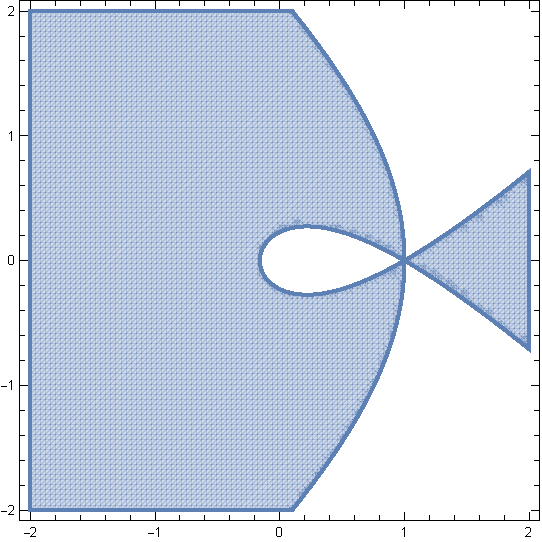
\includegraphics[height=.3\textwidth]{pictures/ReS_edge.pdf}
    \caption{The plot of the region $\operatorname{Re}S(z)-\operatorname{Re}S(1)>0$
			at the edge, in the neighborhood of the double critical point $w_c=1$.
			The new $w$ contour should pass through the shaded region,
		and the new $z$ must stay in the non-shaded region.}
    \label{lecture11:fig:ReS_edge}
\end{figure}
Note however that the old $z$ contour must encircle $z=a$ and $z=0$,
and $z=a$ is a pole of the integrand. The $w$ contour must always be to the right of
the $z$ contour.

We see that there are three regimes, which we consider in the next three subsections.
\subsection{Airy kernel}
	If $a<1$, we can deform the $z$ contour to encircle $z=0$ and $z=a$,
		and the $w$ contour to pass through $w=1$. This will lead to the Airy kernel,
		and the derivation is the same as in
		\Cref{chap:lecture7}.
		We obtain\footnote{Here and below, we understand the convergence
			of the kernels is up to a gauge transformation of the form
		$K(x,y)\mapsto\frac{f(x)}{f(y)}K(x,y)$.}
		\begin{equation*}
			z=1+\frac{Z}{n^{1/3}},\quad w=1+\frac{W}{n^{1/3}},\qquad
			x'=\frac{\xi}{n^{1/6}}, \quad y'=\frac{\eta}{n^{1/6}},
			\qquad
			\frac{1}{n^{1/6}}K_n\to K_{\mathrm{Airy}}(\xi,\eta).
		\end{equation*}
		Here
		\[
			K_{\mathrm{Airy}}(\xi,\eta)=
			\frac{1}{(2\pi i)^2}\iint \frac{\exp\left\{ \frac{W^3}{3}-\xi W-\frac{Z^3}{3}+\eta Z \right\}}{W-Z}\,dW\,dZ.
		\]
		Indeed, the only one new thing that happens here is that $a<1$, and so
		\begin{equation}
			\label{lecture11:eq:z-w-extra-factor}
			\frac{w-a}{z-a}=\frac{1-a+W/n^{1/3}}{1-a+Z/n^{1/3}}=1+O(n^{-1/3}),
		\end{equation}
		so this term does not contribute to the asymptotics of the kernel.

\subsection{BBP transition and the deformed Airy kernel}

		If $a=1$, the behavior is going to be critical --- we still will
		be able to get the same scaling, but the limiting kernel will be different.
		Moreover, looking at \eqref{lecture11:eq:z-w-extra-factor}, we see that
		we need to critically rescale $a$, so
		\begin{equation*}
			a=1+A n^{-1/3},
			\qquad
			\frac{w-a}{z-a}=\frac{W-A}{Z-A}+O(n^{-4/3}),
			\qquad
			\frac{1}{n^{1/6}}K_n\to \tilde K_{\mathrm{Airy}}(\xi,\eta),
		\end{equation*}
		where
		\begin{equation*}
			\tilde K_{\mathrm{Airy}}(\xi,\eta)=
			\frac{1}{(2\pi i)^2}\iint \frac{\exp\left\{
			\frac{W^3}{3}-\xi W-\frac{Z^3}{3}+\eta Z
			\right\}}{W-Z}
			\frac{W-A}{Z-A}
			\,dW\,dZ.
		\end{equation*}
		This kernel is the BBP transition kernel,
		first obtained in the seminal paper by
		Baik--Ben Arous--P\'ech\'e~\cite{BBP2005phase}.
		The spiked top eigenvalue distribution (and the Tracy--Widom distribution)
		are widely used in statistics of high-dimensional,
		highly correlated data.

\subsection{Gaussian regime}
\label{lecture11:sec:gaussian-regime}

Finally, for $a>1$, we cannot deform the integration contours so that they
pass through the double critical point $w_c=1$.
Instead, we can make the contours pass through the point $a$ itself,
and scale the integration variables $w,z$ around $a$ on the scale $n^{-1/2}$ and
not $n^{-1/3}$.

Moreover, we need to make $x,y$ to scale around a different location
instead of $2\sqrt n$. We can find this location by first considering
$x=c\sqrt n$ and expanding as $n\to\infty$:
\begin{multline*}
	n\left( \frac{w^2}{2}-yw/\sqrt{n}+\log w \right)\Big\vert_{w=a+W/\sqrt n,\ y=c\sqrt n+\eta}\\=
	n \left(\frac{a^2}{2}-a c+\log (a)\right)+\sqrt{n} \left(-a \eta +a W+\frac{W}{a}-c W\right)-
	\frac{W^2}{2 a^2}+\frac{W^2}{2}-\eta  W.
\end{multline*}
The term by $n$ is the same in $S(w)$ and $S(z)$ and thus cancels out.
The term by $\sqrt n$ depends on $W$ and cannot be simply removed by a gauge transformation,
so we need to match $c$. We have
\begin{equation*}
	c=a+\frac{1}{a}.
\end{equation*}
\begin{remark}
	You can go to \url{https://lpetrov.cc/simulations/2025-01-28-bbp-transition/}
	and set the parameter $\theta$ (which is the same as $a$)
	to an integer, make $N$ large, and check that the location of the top or bottom eigenvalue
	becomes exactly $a+1/a$. (Despite the fact that the simulation at the link is for $\beta=1$.)
\end{remark}
Setting $c=a+1/a$, we have
\begin{equation*}
	n\ssp S\sim -\frac{W^2}{2 a^2}+\frac{W^2}{2}-\eta  W,
\end{equation*}
and thus the distribution of the top eigenvalue is given by
a Fredholm determinant with the kernel
\begin{equation*}
	K_G(\xi,\eta)=
	\frac{1}{(2\pi)^2}
	\int \int
	\exp\left\{
		\frac{a^{-2}-1}{2}(Z^2-W^2)-\eta W+\xi Z
	\right\}\cdot
	\frac{W}{Z}\cdot
	\frac{dW\,dZ}{W-Z}
\end{equation*}
Note that the factor $\sqrt n$ in front of $K_t$ is precisely
removed by the scaling of $w,z$, and there is no additional scaling
coming from the map $(x,y)\mapsto (\xi,\eta)$.
The contribution
from $(w-a)/(z-a)$ becomes $W/Z$.

The integration contours in $K_G$ are
such that $Re (W^2)>0$ and $Re (Z^2)<0$ on them, and this can be achieved by
the contour deformation.
Indeed, in the new variables, the
behavior at $W=Z=0$ is quadratic, so the
$Z$ contour must pass on the left, and the $W$ contour must be on the right.
One can check that this contour deformation is possible.

\begin{figure}[htpb]
    \centering
    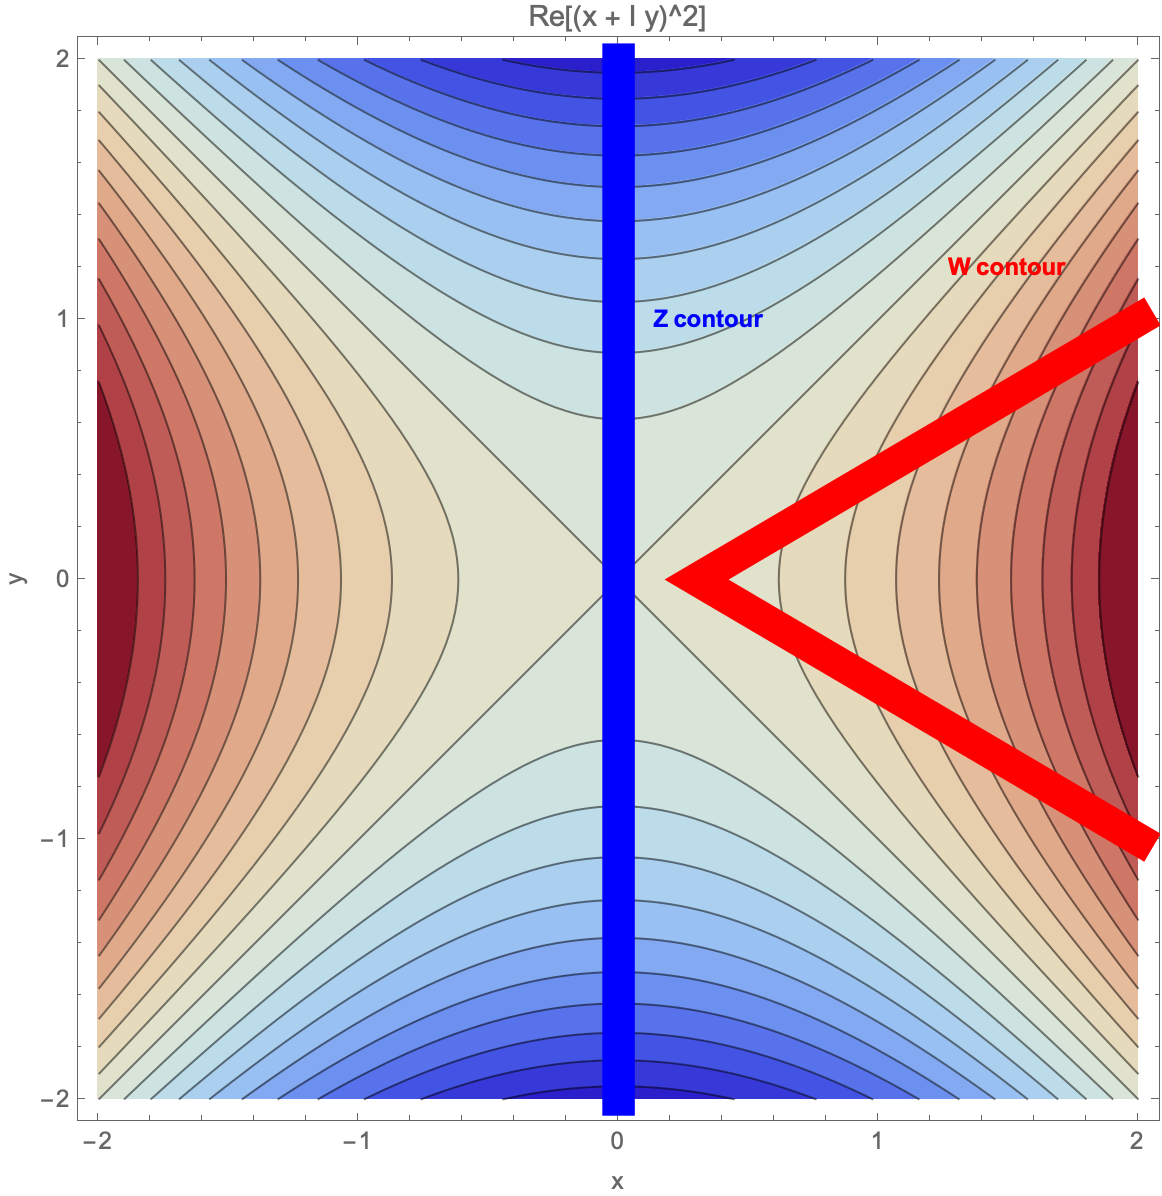
\includegraphics[height=.4\textwidth]{pictures/ReS_Gauss.png}
    \caption{The contour plot of
		$\Re(Z^2)$ around zero. Blue shades correspond to negative values, and yellow to positive. The
		$Z$ contour must pass through the blue region and becomes vertical, and the
		$W$ contour must stay in the yellow region, and becomes a union of two half-lines,
		which are at the angle $<\frac{\pi}{4}$ from the real line.}
		\label{lecture11:fig:ReS_Gauss}
\end{figure}

\subsection{Matching Fredholm determinant to the Gaussian distribution}
\label{lecture11:sec:matching-Gaussian}

Let us renormalize the integration variables
to remove the factor $a^{-2}-1$ in front of the squares,
and match $\det\left( 1-K_G \right)_{\ge x}$ to the Gaussian distribution
(see also Problem~\ref{lecture11:prob:GUE-kernel} for another way to match).
We will work with
\begin{equation*}
	K_G(\xi,\eta)=
	\frac{1}{(2\pi)^2}
	\int \int
	\exp\left\{
		\frac{1}{2}(Z^2-W^2)-\eta W+\xi Z
	\right\}\cdot
	\frac{W}{Z}\cdot
	\frac{dW\,dZ}{W-Z}
\end{equation*}
The discussion below is informal, but can be easily made rigorous.

\medskip

\noindent\textbf{Step 1. Partial fractions and decomposition.}
Observe that
\[
\frac{W}{Z(W-Z)} \;=\;
\frac{1}{Z}\;+\;\frac{1}{\,W-Z\,}.
\]
Thus we can write
\[
K_G(\xi,\eta)
=
K^{(1)}(\xi,\eta)+K^{(2)}(\xi,\eta),
\]
where
\begin{align*}
K^{(1)}(\xi,\eta)
&=
\frac{1}{(2\pi)^2}
\int\!\int
\exp\!\Bigl(\tfrac12(Z^2-W^2)+\xi Z-\eta W\Bigr)\,\frac{1}{Z}\,dW\,dZ,
\\
K^{(2)}(\xi,\eta)
&=
\frac{1}{(2\pi)^2}
\int\!\int
\exp\!\Bigl(\tfrac12(Z^2-W^2)+\xi Z-\eta W\Bigr)\,\frac{1}{W-Z}\,dW\,dZ.
\end{align*}
The term $K^{(1)}$ has a factor $\frac{1}{Z}$ independent of $W-Z$,
while $K^{(2)}$ contains the remaining part $\frac{1}{\,W-Z\,}$.

\medskip

\noindent\textbf{Step 2. Analysis of $K^{(1)}$.}
Focus on
\[
K^{(1)}(\xi,\eta)
=
\frac{1}{(2\pi)^2}
\Bigl(\int
e^{\frac12Z^2+\xi Z}\,\frac{dZ}{Z}\Bigr)
\Bigl(\int
e^{-\frac12W^2-\eta W}\,dW\Bigr).
\]
The operator $K^{(1)}$ is a rank-1 operator in the variables $\xi,\eta$:
\[
K^{(1)}(\xi,\eta)
=
u(\xi)\,v(\eta)
\]
for some functions $u(\cdot)$ and $v(\cdot)$ of one variable each.
Hence $K^{(1)}$ has at most one nonzero eigenvalue (its trace).

\medskip

\noindent\textbf{Step 3. Representation of $K^{(2)}$ and the key identity.}
For $K^{(2)}$, we use
\[
\frac{1}{\,W-Z\,}=\int_0^{\infty} e^{-t(W-Z)}\,dt
\]
(again justified by the choice of integration contours). Then
\[
K^{(2)}(\xi,\eta)
=
\int_0^\infty
\Bigl[
\frac{1}{2\pi i}\!\int
e^{\frac12Z^2+(\xi+t)Z}\,dZ
\Bigr]
\Bigl[
\frac{1}{2\pi i}\!\int
e^{-\frac12W^2-(\eta+t)W}\,dW
\Bigr]dt.
\]
Denote
\[
A(\xi,t)
=
\frac{1}{2\pi i}\int
e^{\frac12Z^2+(\xi+t)Z}\,dZ,
\quad
B(t,\eta)
=
\frac{1}{2\pi i}\int
e^{-\tfrac12W^2-(\eta+t)W}\,dW.
\]
Hence
\(
K^{(2)}(\xi,\eta)=\int_0^\infty A(\xi,t)\,B(t,\eta)\,dt.
\)
In operator form on suitable spaces,
this reads $K^{(2)}=A\,B$, and one checks $B\,A=I$
(\emph{identity on the $t$-variable space}),
so $A\,B$ and $B\,A$ share the same nonzero spectrum.
Indeed,
\begin{equation*}
	BA(s,t)=\frac{1}{(2\pi i)^2}
	\int_{\mathbb{R}}d\xi
	\int dW\, dZ
	e^{-\frac{1}{2}W^2+\frac{1}{2}Z^2}
	e^{-(s+\xi)W+(\xi+t)Z}.
\end{equation*}
Integrating over $\xi$ in the Fourier sense yields the delta:
\begin{equation*}
	\int_{\mathbb{R}}d\xi e^{\xi(Z-W)}=2\pi\delta(Z-W).
\end{equation*}
Integrating in $W$ is again an integral of $e^{(t-s)W}$, and thus, the second $2\pi$ disappears,
and we arrive at $BA(s,t)=\delta(s-t)$, which is the kernel of the identity operator.

We conclude that $AB$ is a projection, since
$(AB)^2=ABAB=AB$.

\medskip
For the rest of 
the analysis, continue to
Problem~\ref{lecture11:prob:Gaussian_kernel}.









\section{Problems}


\subsection{Biorthogonal ensembles}
\label{lecture11:prob:biorthogonal}

Derive \Cref{lecture11:thm:dbm-det-kernel} from
\Cref{lecture11:lem:density_representation}
using the orthogonalization process similar
to~\Cref{chap:lecture5},
and then taking the limit as $s\to\infty$.

\subsection{Scaling of the kernel}
\label{lecture11:prob:scaling}

Let $a_i=0$ in \Cref{lecture11:thm:dbm-det-kernel}.
Find $\alpha$ such that
$t^\alpha K_t(x/\sqrt{t},y/\sqrt{t})$ is independent of $t$.
Can you explain this value of $\alpha$?

\subsection{Gaussian regime and integration contours}

Check that the contour deformation
from $(z,w)$ to $(Z,W)$ passing through $a$
described in
\Cref{lecture11:sec:gaussian-regime} is valid.

\subsection{Gaussian kernel}
\label{lecture11:prob:Gaussian_kernel}

Finish the proof of the Fredholm determinant representation
of the Gaussian cumulative distribution function
by manipulation with Fredholm determinants, which was started in
\Cref{lecture11:sec:matching-Gaussian}.

\subsection{GUE kernel}
\label{lecture11:prob:GUE-kernel}

Consider the following generalization of the kernel $K_G$
from \Cref{lecture11:sec:gaussian-regime}:
\begin{equation*}
	K_G^m(\xi,\eta)=
	\frac{1}{(2\pi)^2}
	\int \int
	\exp\left\{
		\frac{1}{2}(Z^2-W^2)-\eta W+\xi Z
	\right\}\cdot
	\left(
	\frac{W}{Z}
\right)^{m}
\frac{dW\,dZ}{W-Z},
\end{equation*}
where $m\ge1$ is an integer and the contours are as in \Cref{lecture11:fig:ReS_Gauss}.
Show that the Fredholm determinant
$\det\left( 1-K_G^m \right)_{L^2(x,+\infty)}$
is the cumulative distribution function of the largest eigenvalue
of the $m\times m$ GUE matrix,
that is, $\operatorname{\mathbb{P}}(\lambda_{\max}^{(m\times m)}\le x)$.














\chapter{Random Growth Models}
\label{chap:lecture12}





\section{Recap}

In our last lecture, we explored the asymptotics of Dyson Brownian Motion with an outlier. We specifically focused on the phase transition that occurs when a rank-1 perturbation is applied to a random matrix ensemble.

\subsection{Dyson Brownian Motion with Determinantal Structure}

We established that for $\beta=2$, the eigenvalues of the time-evolved process form a determinantal point process. The transition probability from an initial configuration $\mathbf{a} = (a_1 \geq \cdots \geq a_N)$ to a configuration $\mathbf{x} = (x_1 \geq \cdots \geq x_N)$ at time $t$ is given by:
\begin{equation*}
P(\lambda(t) = \mathbf{x} \mid \lambda(0) = \mathbf{a}) = N! \Big(\frac{1}{\sqrt{2\pi t}}\Big)^N \prod_{1\leq i<j\leq N}\frac{x_i - x_j}{a_i - a_j} \det\Big[\exp\Big(-\frac{(x_i - a_j)^2}{2t}\Big)\Big]_{i,j=1}^N
\end{equation*}

This determinantal structure enabled us to derive the correlation kernel:
\begin{equation}\label{lecture12:eq:correlation-kernel}
K_t(x,y) = \frac{1}{(2\pi)^2 t} \int\int \exp\Big(\frac{w^2 - 2yw}{2t}\Big) \bigg/ \exp\Big(\frac{z^2 - 2xz}{2t}\Big) \prod_{i=1}^n \frac{w-a_i}{z-a_i} \frac{dw\,dz}{w-z}
\end{equation}
where the contours of integration are specified to maintain analytical properties.

\subsection{The BBP Phase Transition}

The central focus was the Baik-Ben Arous-Péché (BBP) phase transition that occurs with finite-rank perturbations of GUE matrices. For the rank-1 case, we analyzed:
\begin{equation*}
A + \sqrt{t}G, \quad \text{where } A = \text{diag}(a\sqrt{n},0,\ldots,0)
\end{equation*}

Through asymptotic analysis using steepest descent methods, we identified three distinct regimes:

\begin{enumerate}
\item \textbf{Airy regime} ($a < 1$): The largest eigenvalue follows the Tracy-Widom GUE distribution, just as in the unperturbed case. The spike is too weak to escape the bulk.

\item \textbf{Critical regime} ($a = 1$): A transitional behavior occurs when $a = 1 + An^{-1/3}$, leading to a deformed Airy kernel:
\begin{equation*}
\tilde{K}_{\text{Airy}}(\xi,\eta) = \frac{1}{(2\pi i)^2}\iint \frac{\exp\left\{\frac{W^3}{3}-\xi W-\frac{Z^3}{3}+\eta Z\right\}}{W-Z} \frac{W-A}{Z-A} dW\,dZ
\end{equation*}

\item \textbf{Gaussian regime} ($a > 1$): The largest eigenvalue separates from the bulk, becoming an "outlier" centered at $a + 1/a$. Its fluctuations follow a Gaussian distribution rather than the Tracy-Widom law.
\end{enumerate}


\subsection{Remark: Corners process with outliers}

One can also perturb the corners process structure, and get
correlation kernels similar to \eqref{lecture12:eq:correlation-kernel}
which we had for the Dyson Brownian Motion.
The perturbed corners process is
considered in \cite{Ferrari2014PerturbedGUE},
see also the earlier work \cite{Metcalfe2011GT}
for the corners process of $UDU^\dagger$, where $D$ is arbitrary and
$U$ is Haar-distributed. Both the kernels
for the Dyson Brownian Motion and the corners process
with outliers can be obtained from the formula of
\cite{Metcalfe2011GT}.
See \Cref{lecture12:fig:outlier-evolution} for an illustration of the corners process with an outlier
in two cases, when the basis for the outlier is rotated or not
(the rotation does not affect the top level eigenvalue distribution,
but has a significant effect on the whole corners process).




\begin{figure}[]
	\centering
	\begin{tabular}{cc}
		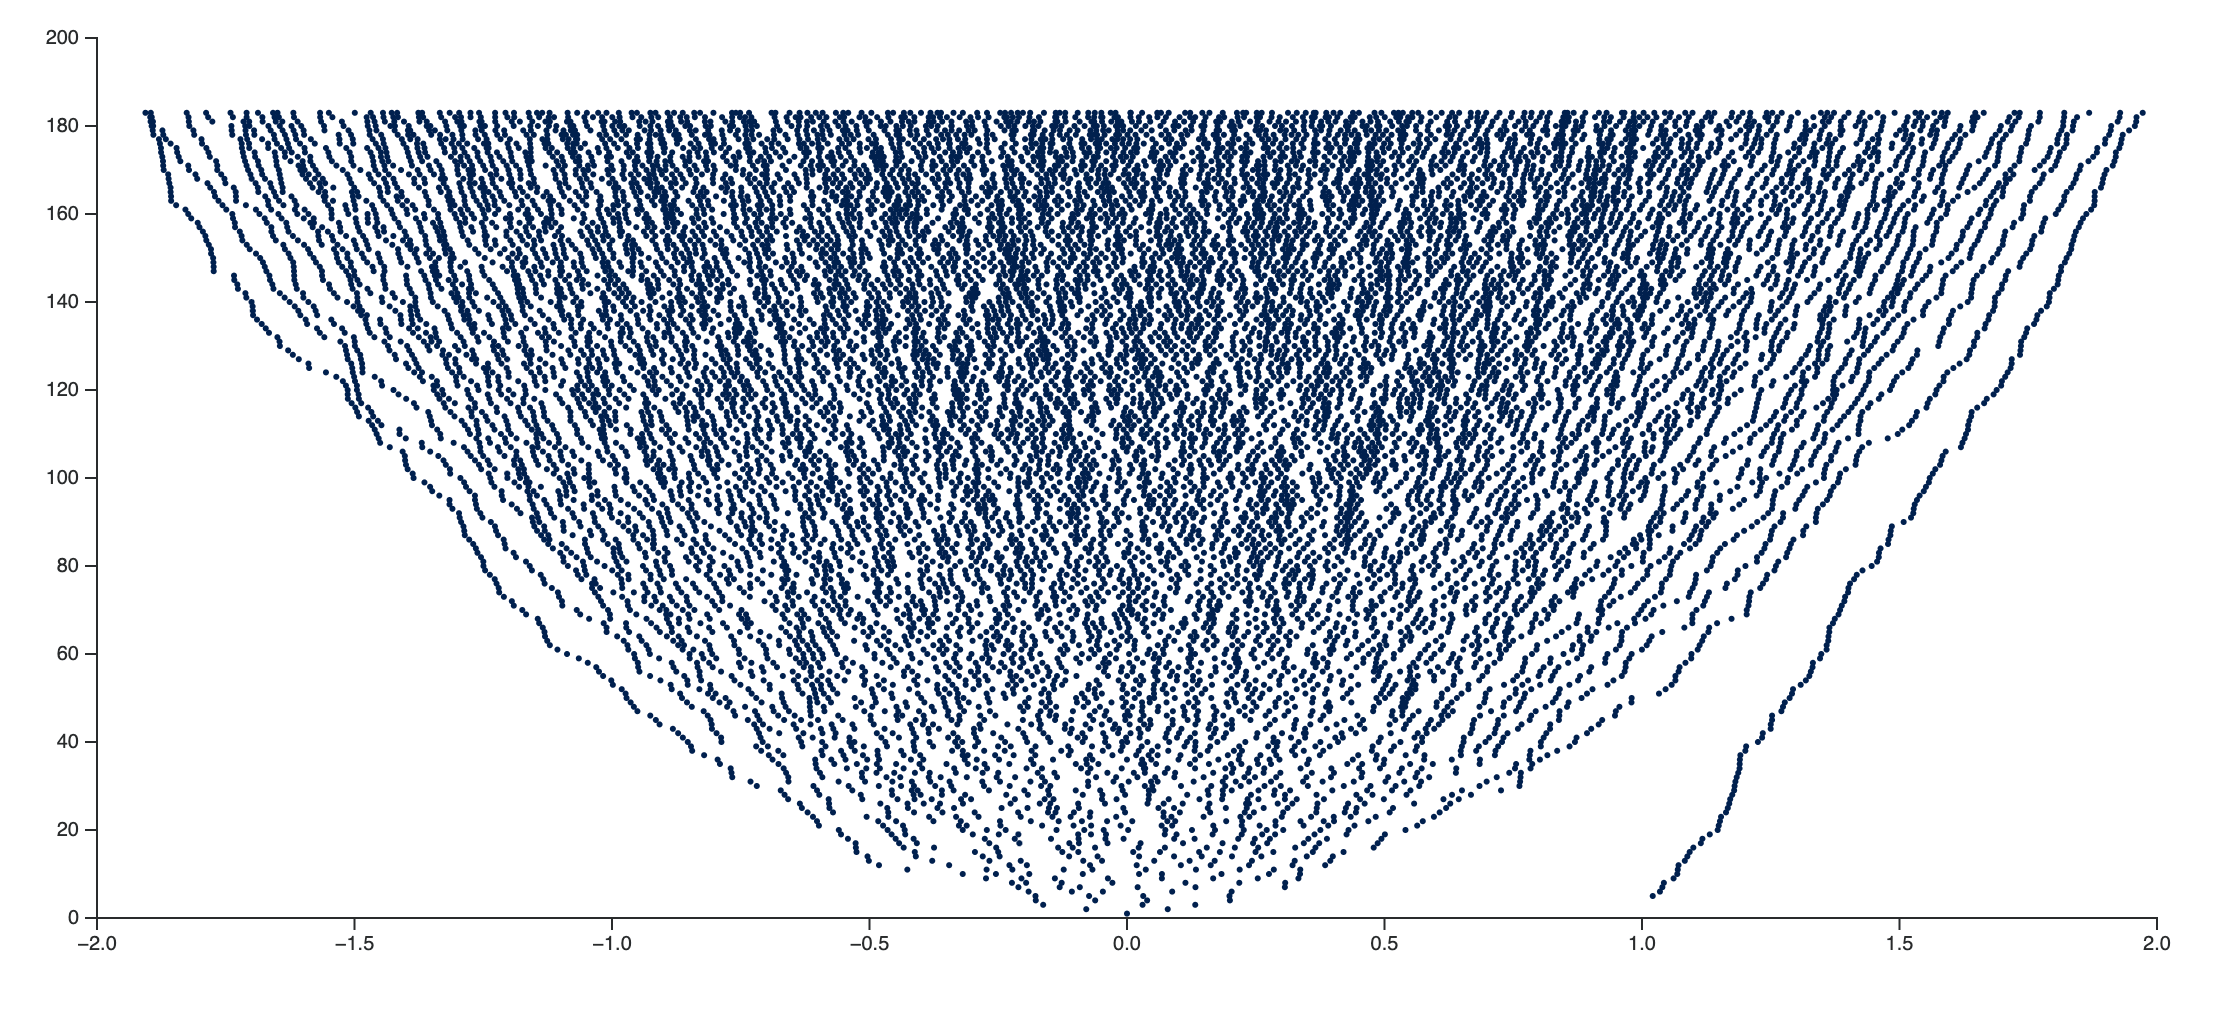
\includegraphics[width=0.45\textwidth]{pictures/outlier.png} &
		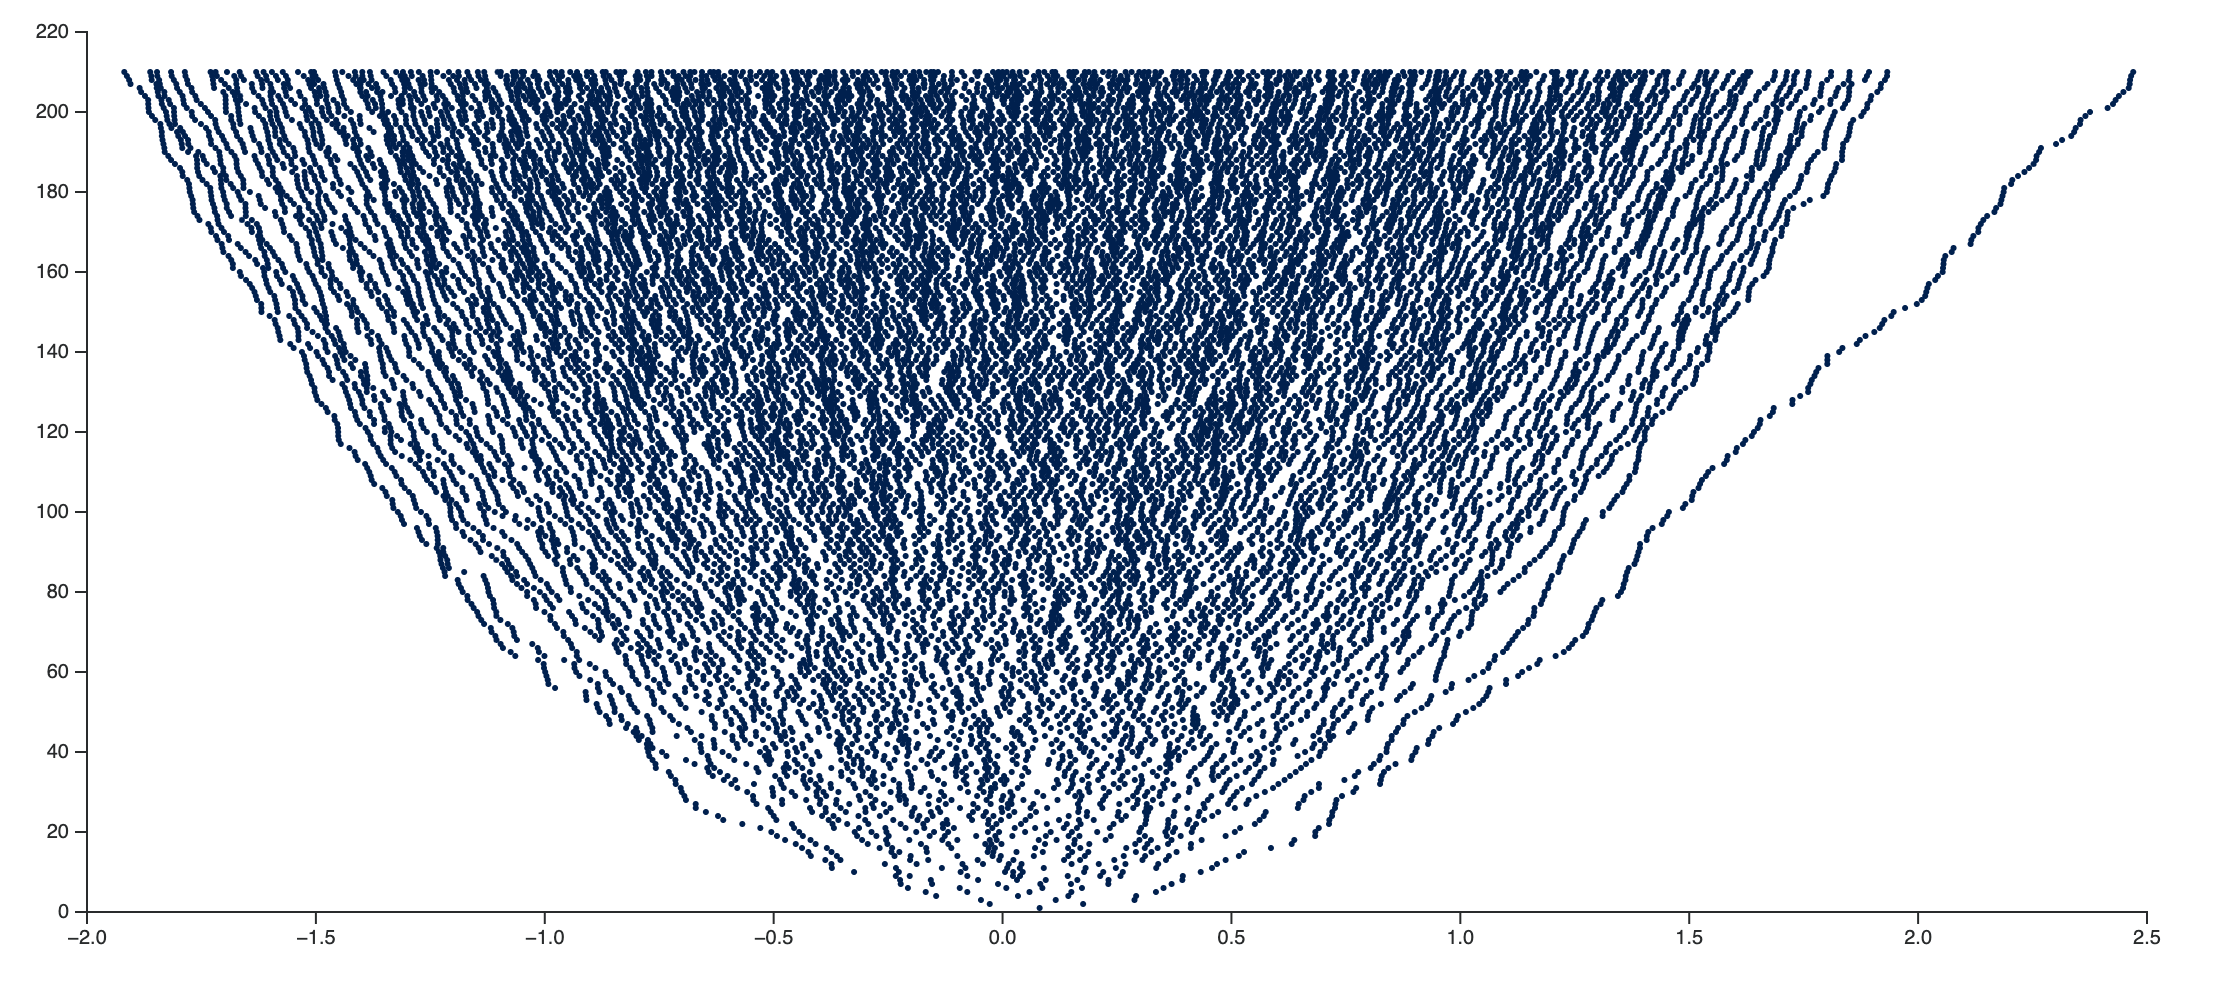
\includegraphics[width=0.45\textwidth]{pictures/rotated_outlier.png}
	\end{tabular}
	\caption{Two versions of the corners process with an outlier.
	Left: Corners process of $G+D$, where $D$ is a rank-1 critical perturbation with eigenvalue
	$1$. Right: Corners process of $G+UDU^\dagger$, where
	$U\in U(n)$ is a Haar-distributed unitary matrix and $D$
	is a rank-1 supercritical perturbation with eigenvalue $2$
	(the eigenvalue $1$ is not visible in the rotated system).
	In both pictures, $n\approx 200$. See
	\url{https://lpetrov.cc/simulations/2025-03-27-orthogonal-corners-outliers/}
	for an interactive simulation.}
	\label{lecture12:fig:outlier-evolution}
\end{figure}


\subsection{Goal today}

Today, the goal is to survey various objects which arise in the KPZ universality class:
\begin{itemize}
	\item
		The Airy line ensemble, which is
		the universal edge scaling limit of Dyson Brownian Motion,
		the corners process, and numerous statistical physics models.

	\item
		Moreover, the Airy line ensemble arises and
		is fundamental for a class of random growth models
		in one space and one time dimensions, which is known as the KPZ universality class.

	\item
		We will briefly mention how the Gaussian Free Field (GFF) arises in the KPZ class
		models in two space dimensions.

	\item
		We continue to discuss one particular model in the KPZ universality
		class --- the Polynuclear Growth (PNG) and the related Last Passage Percolation (LPP) models.
\end{itemize}

\section{A window into universality: Airy line ensemble}

The edge scaling limit of Dyson Brownian Motion
and the corners process\footnote{Both without outliers --- the presence of
critical outliers may add a few extra lines (wanderers) to the Airy line ensemble,
and we will not consider this complication here.}
is a universal object for $\beta=2$ models and determinantal structures (and far beyond).
GUE formulas
provide us with a powerful lens through which to examine these universality phenomena. In this section, we discuss the limiting behavior of Dyson Brownian Motion near the spectral edge, highlighting two of its fundamental properties: Brownian Gibbs property and characterization.

\begin{theorem}[Edge scaling limit to Airy line ensemble]
	Consider an $N\times N$ GUE (Gaussian Unitary Ensemble) Dyson Brownian motion, i.e., the stochastic process of eigenvalues $(\lambda_1(t)\ge \cdots\ge \lambda_N(t))_{t\in\mathbb{R}}$ evolving under Dyson's eigenvalue dynamics. After centering at the spectral edge parallel to the vector $\mathbf{v}_t$ and applying the
Airy scaling (tangent axis scaled by $N^{-1/3}$ and fluctuations scaled by $N^{-1/6}$), the top $k$ eigenvalue trajectories converge as $N\to\infty$ to the \textbf{Airy line ensemble}. In particular, for each fixed $k\ge1$ the rescaled process $$(N^{1/6}[\lambda_i(\langle
			N^{-1/3},N^{-1/6}
\rangle \cdot \mathbf{v})-c_{N,t}])_{1\le i\le k}$$ converges in distribution (uniformly on compact $t$-intervals) to $(\mathcal{P}_i(t))_{1\le i\le k}$, where $\{\mathcal{P}_i(t)\}_{i\ge1}$ is the parabolic Airy line ensemble.
\end{theorem}

\begin{remark}
	The random variable $\mathcal{P}_1(0)$ has the GUE Tracy-Widom distribution.
\end{remark}

\begin{theorem}[Airy line ensemble is Brownian Gibbsian \cite{CorwinHammond2013}]
The parabolic Airy line ensemble
$\{\mathcal{P}_i(t)\}_{i\ge1}$ satisfies the
\textbf{Brownian Gibbs property}. Namely, for any fixed
index $k\ge1$ and any finite time interval $[a,b]$,
conditioning on the outside portions of the ensemble (i.e.,
$\{\mathcal{P}_j(t): t\notin[a,b]\}$ for all $j$, and
$\{\mathcal{P}_j(t): j\neq k\}$ for $t\in[a,b]$), the
conditional law of the $k$th curve on $[a,b]$ is that of a
\textbf{Brownian bridge} from $(a,\mathcal{P}_k(a))$ to
$(b,\mathcal{P}_k(b))$ \textbf{conditioned} to stay above
the $(k+1)$th curve and below the $(k-1)$th curve on
$[a,b]$. In particular, the Airy line ensemble is invariant
under this resampling of a single curve by a conditioned
Brownian bridge.
\end{theorem}

\begin{theorem}[Characterization of ALE \cite{AggarwalHuang2023Characterization}]
	The parabolic Airy line ensemble is the \textbf{unique}
	Brownian Gibbs line ensemble satisfying a natural
	parabolic curvature condition on the top curve. More
	precisely, let
	$\boldsymbol{\mathcal{P}}=(\mathcal{P}_1,\mathcal{P}_2,\ldots)$
	be any line ensemble that satisfies the Brownian Gibbs
	property. Suppose in addition that the top line
	$\mathcal{P}_1(t)$ \textbf{approaches a parabola} of
	curvature $1/\sqrt{2}$ at infinity. Then
	$\boldsymbol{\mathcal{L}}$ must coincide (in law) with the
	\textbf{parabolic Airy line ensemble}, up to an overall
	affine shift of the entire ensemble.
\end{theorem}

Let us define $\mathcal{L}_i(t)=\mathcal{P}_i(t)+t^2$, and
call $\mathcal{L}$ the Airy Line Ensemble
(without the word ``parabolic''). One can think that the parabola comes
from the scaling window, which is of different proportions
in the horizontal and vertical directions.
The non-parabolic
Airy line ensemble $\mathcal{L}$ is time-stationary,
that is, its distribution is invariant under time shifts $t\mapsto t+c$.

\section{KPZ universality class: Scaling and fluctuations}

\subsection{Universality of random growth}

In the $(1+1)$-dimensional \textbf{KPZ universality class},
random growth models exhibit a distinctive scale of
fluctuations fundamentally different from classical Gaussian
behavior. Kardar, Parisi, and Zhang \cite{KPZ1986} predicted
that such interfaces have \emph{roughness exponent} $1/2$
and \emph{growth exponent} $1/3$, meaning that if time is
scaled by a factor $T$, then horizontal distances scale by
$T^{2/3}$ and vertical height fluctuations scale by
$T^{1/3}$ \cite{remenik2023integrable}, as $T\to\infty$.
Equivalently, the interface height $h(t,x)$ (after subtracting its deterministic mean growth) satisfies the \emph{$1:2:3$ scaling}:
\[ t^{-1/3}\left(
h(t,\chi t^{2/3})-\mathbb{E}[h(t, \chi t^{2/3})]
\right)\qquad \textnormal{converges in law as } t\to\infty.
\]
These exponents $2/3$ and $1/3$ are universal in
one-dimensional growth with local randomness, distinguishing
the KPZ class from, e.g., diffusive (Edwards–Wilkinson)
interfaces. Intuitively, the interface develops random peaks
of size $O(t^{1/3})$, and correlations spread over a spatial
range $O(t^{2/3})$—a highly nontrivial, super-diffusive
scaling.

\subsection{KPZ equation}

The KPZ equation is a continuous model of random growth which was first proposed
non-rigorously in the physics literature \cite{KPZ1986}, and then
justified mathematically. There are several justifications,
including the one by Hairer \cite{Hairer11}.
The equation reads (ignoring the constant by the terms in the right-hand side):
\begin{equation}
	\label{lecture12:eq:KPZ}
	\partial_t h(t,x) = \partial_{xx} h(t,x)+\big(\partial_x h(t,x)\big)^2 + \xi(t,x),
	\qquad t>0,\quad x\in\mathbb{R},
\end{equation}
where $\xi$ is the space-time white noise, that is, a Gaussian process with
\begin{equation*}
	\operatorname{\mathbb{E}}[\xi(t,x)\xi(t',x')] = \delta(t-t')\delta(x-x').
\end{equation*}
The terms in the KPZ equation stand for the three types of interactions
driving the random growth process:
\begin{itemize}
	\item The first term $\partial_{xx} h$ is a
		\emph{smoothing} heat equation term, which is a
		classical diffusion (independent growth) term.
	\item The second term $\big(\partial_x h\big)^2$ is a \emph{slope-dependent growth} term, which
		tends to close high-slope gaps. This mechanism is visible in discrete models
		which we will see in \Cref{lecture12:sec:PNG}.
	\item The third term $\xi(t,x)$ is a \emph{stochastic noise} term
		which favors independent growth at each location.
		This leads to roughening of the interface.
\end{itemize}

Note that the equation \eqref{lecture12:eq:KPZ}
is ill-posed even in the sense of distributions,
since squaring a distribution $\partial_x h$ is not well-defined.
Instead, to solve the KPZ equation in one space dimension $x\in\mathbb{R}$,
one can formally write $h=\log Z$, where $Z$ then solves the well-posed
\emph{stochastic heat equation} (SHE) with multiplicative noise:
\begin{equation*}
	\partial_t Z(t,x) = \partial_{xx} Z(t,x) + \xi(t,x)Z(t,x).
\end{equation*}
The stochastic heat equation is linear in $Z$, and there are no issues with
defining the solution. The passage from $h$ to $Z=\exp(h)$ is known as the
\emph{Cole-Hopf transformation}. It is not rigorous either, but
was used prior to \cite{Hairer11} to define what it means to have a solution
to \eqref{lecture12:eq:KPZ}.

\subsection{First discoveries}

One of the most striking discoveries is that the
\textbf{one-point distribution} of these fluctuations,
when the growth starts from the so-called
\emph{droplet} (or \emph{narrow wedge}) initial condition,
is
governed by the GUE \emph{Tracy–Widom law},
rather than a normal law. The \textbf{Tracy–Widom
distribution} (for Gaussian Unitary Ensemble, GUE) describes
the fluctuations of the largest eigenvalue of a random
Hermitian matrix. In the KPZ class, the same distribution
emerges in the long-time limit for a wide range of models
and initial conditions. For example,
in the Totally Asymmetric Simple Exclusion Process
(TASEP) with step initial data (corresponding to the narrow wedge), the height at the
origin, when centered and scaled by $t^{1/3}$, converges in
law to the Tracy–Widom GUE distribution
\cite{johansson2000shape},
\cite{remenik2023integrable}.
This was the first rigorous confirmation of $1/3$
fluctuations in a random growth model.
Such behavior is believed
to be \emph{universal}: many other integrable models
(polynuclear growth, last-passage percolation, directed
polymers, etc.) exhibit the same long-time distribution and
scaling exponents.

In the next \Cref{lecture12:sec:PNG}, we will discuss a particular semi-discrete random
growth model --- the Polynuclear Growth (PNG).

\subsection{Effect of initial conditions}

Crucially, the exact form of the limiting distribution depends on the \emph{initial condition} of the growth process. Different symmetry classes of random matrices appear:
\begin{itemize}
		\item \textbf{Curved (droplet) initial data:} Starting
			from a narrow peak (often called \emph{narrow wedge}
			or droplet initial condition), the height fluctuations
			follow the Tracy--Widom GUE distribution in the
			$t\to\infty$ limit. This
			corresponds to the \emph{unitary} symmetry
			class (e.g. complex Hermitian matrices).

		\item \textbf{Flat initial data:} Starting from a flat
			interface (e.g. all zero initial height), fluctuations
			converge to the Tracy--Widom GOE distribution,
			which is the law of the
			largest eigenvalue of a random real symmetric (Gaussian
			orthogonal ensemble) matrices, with \emph{orthogonal} symmetry.

		\item \textbf{Stationary initial data:} Starting from a
			two-sided Brownian or otherwise stationary initial
			profile, the fluctuation distribution is
			again non-Gaussian but neither GOE nor GUE. In this
			case one obtains the \emph{Baik--Rains distribution},
			often denoted $F_0$, which was first derived by Baik
			and Rains for a stationary last passage percolation
			model \cite{baik2000limiting_BR_distribution}.
\end{itemize}

\subsection{Remark: Gaussian Free Field in KPZ universality}

The KPZ equation \eqref{lecture12:eq:KPZ} can be posed in any space dimension:
\begin{equation*}
	\partial_t h(t,x)= D h(t,x) + (\nabla h(t,x))^2 + \xi(t,x),
	\qquad t>0,\quad x\in\mathbb{R}^d,
\end{equation*}
where $D$ is a second-order differential operator, and $\nabla$ is the gradient.
In $d=2$ case, the operator $D$ can have one of the two signatures:
\begin{equation*}
	D=\Delta \quad \text{or} \quad D=\partial_x^2-\partial_y^2.
\end{equation*}
These two cases are known as \emph{isotropic} and \emph{anisotropic} KPZ equations, respectively.

The isotropic KPZ equation is much more mysterious than the anisotropic one.
In the anisotropic case, it is believed that the
fluctuations scale with exponent $0$
(as opposed to $1/3$ for one dimension),
while in the isotropic case, even the hypothetical fluctuation scaling exponent is debated.

Further evidence for the anisotropic case is the existence of exactly
solvable growth models in this class (e.g., \cite{BorFerr2008DF}),
which have logarithmic fluctuations. Moreover, their fluctuations
are governed by the Gaussian Free Field (GFF), which we encountered earlier in
\href{https://lpetrov.cc/rmt25/rmt2025-l9.pdf}{Lecture 9}.
Moreover, the GFF should be the stationary distribution for the anisotropic
KPZ fixed point (Markov process which should be the long-time scaling limit
of the anisotropic KPZ equation).

Back to random matrices, consider the following question:
\begin{quote}
	Can we imagine a 2-dimensional random growth model
	on random matrices, which will look like the 2-dimensional anisotropic KPZ equation?
	It would have random growth features, where some 2-dimensional surface is growing,
	and will have the GFF fluctuations.
\end{quote}

We know an object in random matrices
with GFF fluctuations --- the height function of the corners process.
So, a natural guess is to take the Brownian motion on matrix elements,
and look at the evolution of the corners eigenvalues. However,
the evolution of the eigenvalues of all corners is \emph{not}
going to be Markov.
A workaround is the construction by Warren \cite{warren2005dyson},
which produces the relevant Markov process on the full
interlacing corners configuration.

\section{Polynuclear Growth and Last Passage Percolation}
\label{lecture12:sec:PNG}

\subsection{Definition and single-layer PNG}
\label{lecture12:sub:PNG-definition}
We start with the \emph{single-layer} PNG model on the real line. The interface height $h(t,x)$ evolves in continuous time $t\ge0$ over the spatial coordinate $x\in\mathbb{R}$ and has piecewise-constant plateaus with sharp upward steps.
In other words, $h(t,x)$ is piecewise constant in $x$, and takes integer values.

\smallskip

\noindent\textbf{Dynamics.} The evolution is described by two basic ingredients:
\begin{enumerate}
\item \emph{Nucleation events:} At random times and locations $(t,x)$ in the plane, a new ``island'' of height 1 is born atop the existing surface. Each newly born island sits just above $h(t,x)$, creating a step of height $1$ at the precise point $x$ and time $t$.
	We assume that the nucleation events form a Poisson process in space-time $(t,x)$.
\item \emph{Lateral spread:} Once an island is created at height $k+1$, its boundaries spread outward (to the left and right in $x$) with speed $1$. Thus a step boundary moves in both directions until it merges with another step boundary or nucleation event.
	When the islands merge, the height becomes flat at this point.
\end{enumerate}
See \Cref{lecture12:fig:PNG} for an illustration of the single-layer PNG model.
See also \Cref{lecture12:fig:png-single}
for an evolution
of the nucleation events, each of which
spreads at speed $1$.

\begin{figure}[htb]
 \centering
 \begin{tikzpicture}[scale=0.9]
 % Axes
 \draw[->] (-4,0) -- (4,0) node[right] {$x$};
 \draw[->] (0,0) -- (0,4) node[above] {$t$};

 % PNG Interface at time t=2 (with up and down steps)
 \draw[thick, blue] (-4,2) -- (-3.5,2) -- (-3.5,2.6) -- (-2,2.6)--++(0,-.6)--++(.1,0)--++(0,-.6)
 --++(1,0)--++(0,.6)--++(1.5,0)--++(0,-0.8)--++(1,0)--++(0,.6)--++(.2,0)--++(0,.6)--++(1.5,0);


 \end{tikzpicture}
 \caption{Polynuclear Growth (PNG) model interface.}
 \label{lecture12:fig:PNG}
\end{figure}


\begin{figure}[htpb]
\centering
\begin{tikzpicture}[scale=0.85,>=stealth, line cap=round, line join=round]
% time axis
\draw[->] (-4.2,0) -- (4.2,0) node[right] {$x$};
\draw[->] (0,0) -- (0,3.5) node[above] {$t$};
% nucleation events
\node[circle, fill=black, inner sep=1pt] (n1) at (1.5,1.1) {};
\node[circle, fill=black, inner sep=1pt] (n2) at (-2.5,1.9) {};
\node[circle, fill=black, inner sep=1pt] (n3) at (-0.5,2.4) {};
% arcs for lateral spread
\draw[thick] plot [domain=1.5-1.1:1.5+1.1] (\x,{1.1+abs(\x-1.5)});
\draw[thick] plot [domain=-2.5-1.6:-2.5+1.6] (\x,{1.9+abs(\x+2.5)});
\draw[thick] plot [domain=-0.5-0.4:-0.5+0.4] (\x,{2.4+abs(\x+0.5)});
% partial interface shape for demonstration
% we only draw several "steps" at certain time slices
% time slice t=3
\draw[dashed] (-4,3) -- (4,3);
\node at (4.25,3) {$t=3$};
% some example step boundary: from roughly -3.5 to -2.5, height 1
% (for illustration only, not exact solution)
\end{tikzpicture}
\caption{Single-layer PNG: Nucleations (black dots) appear randomly in the $(t,x)$ plane
according to a Poisson process. Each nucleation creates an upward step of height $1$. The boundary of each newly created island expands laterally at speed $1$.}
\label{lecture12:fig:png-single}
\end{figure}

\smallskip

\noindent\textbf{Initialization.} One typically imposes an initial condition $h(0,x)$ on the spatial axis (e.g., a single spike or droplet, or a flat interface).
The flat interface is $h(0,x)=0$ for all $x\in\mathbb{R}$, and the droplet is a single upward step at $x=0$ with height $1$. In the droplet case, we also set $h(0,x)=-\infty$ for $x\ne 0$, for
convenience.

\subsection{Multiline PNG}
\label{lecture12:sub:multiline-png}

The \emph{multiline} version of PNG tracks multiple height levels by stacking interfaces
at multiple layers, $h_k(t,x)$. A merging event
at layer $k$ produces a nucleation event at layer $k+1$.
So, the nucleation at $h_1$ is powered by the Poisson process,
while the nucleation at each $h_k$, $k\ge 2$, is powered by the merges at $h_{k-1}$.
The initial condition is assumed to satisfy
\begin{equation*}
	h_1(0,x) \ge h_2(0,x) \ge \cdots ,\qquad \textnormal{for all } x\in\mathbb{R}.
\end{equation*}
This ordering is preserved by the evolution,
see Problem~\ref{lecture12:prob:multiline-png}.

We see that the evolution of $h_2,h_3,\ldots $ is
just a function of the full space-time evolution of $h_1$.
However, at fixed time $t$,
the functions $h_k(t,\cdot)$ cannot be determined
just by $h_1(t,\cdot)$.

The evolution of all the $h_k$'s can be modeled on the same Poisson process plot,
by looking at ``shadow lines'', the lines of the second, third, etc. orders
arising when two lines of the previous order merge.

\subsection{KPZ mechanisms in the PNG growth}

Let us compare the single-layer PNG growth with the ingredients of the KPZ equation
\eqref{lecture12:eq:KPZ}:
\begin{itemize}
	\item Independent nucleation events in the PNG model correspond to the stochastic noise term $\xi(t,x)$ in the KPZ equation.
	\item The lateral spread of step boundaries in PNG is akin to the slope-dependent growth term $(\partial_x h)^2$ in KPZ. Indeed, if the slope is large, the growth at a given point happens with higher speed.
	\item
		The diffusion smoothing mechanism is not quite visible, but one can think of it as the effect of the nucleation events, which are spread out in space and time.
\end{itemize}

\subsection{Last Passage Percolation (LPP)}

Let us now describe the height function $h_1(t,x)$ of the top layer of the PNG model as a
percolation problem in the Poisson environment.
Consider a Cartesian coordinate system with axes $u$ and
$v$. Let $t$
represent the diagonal ``time'' axis, defined as $t = u + v$.
Now, imagine a Poisson point process $\mathcal{P}$ of
intensity $1$ in the upper half-plane $\{(u,v): u\ge 0, v\ge 0\}$.
For two points $(u_1, v_1)$ and $(u_2, v_2)$ with $u_1 \leq
u_2$ and $v_1 \leq v_2$, an up-right path from $(u_1, v_1)$
to $(u_2, v_2)$ is a continuous curve moves only
rightward (increasing $u$) or upward (increasing $v$). The
weight of a path is defined as the number of Poisson points
it collects along the way.

The last passage time $\mathcal{P}[(u_1, v_1) \to (u_2, v_2)]$ is defined as the maximum weight among all up-right paths from $(u_1, v_1)$ to $(u_2, v_2)$:
\begin{equation*}
\mathcal{P}[(u_1, v_1) \to (u_2, v_2)] = \max_{\pi: (u_1, v_1) \to (u_2, v_2)} \#\{\text{Poisson points collected by }\pi\}
\end{equation*}
This maximum is always attained by some piecewise linear path and represents a random variable that depends on the Poisson environment $\mathcal{P}$.

\begin{proposition}
	\label{lecture12:prop:PNG}
For the PNG model with the droplet initial condition, the height function $h_1(t,x)$ at position $x$ and time $t$ can be expressed as:
\begin{equation*}
h_1(t,x) = \mathcal{P}[(0,0) \to (u,v)]
\end{equation*}
where the coordinates $(u,v)$ satisfy $u + v = t$ and $u - v = x$. In other words, the point $(u,v)$ lies on the diagonal "time" line $t = u + v$ at the spatial position corresponding to $x = u - v$.
\end{proposition}
\begin{proof}
	See Problem~\ref{lecture12:prob:PNG_LPP}.
\end{proof}

\subsection{Topics to continue}

\begin{itemize}
	\item Multipath LPP and multi-layer PNG: 
		$h_1+\ldots+h_k $ (with the droplet initial condition)
		has the same distribution as 
		$\mathcal{P}^{(k)}[(0,0)\to (t+x,t-x)]$, the $k$-path point-to-point LPP distribution.
	\item Connection to the Airy line ensemble --- PNG with
		the droplet initial condition converges to the Airy line
		ensemble. (Same it true of the LPP, by the mapping.)
		So, the PNG/LPP with the droplet initial condition 
		is related to Hermitian symmetric random matrices.
	\item PNG with flat initial condition / LPP in the point-to line regime 
		converge to the GOE Tracy-Widom distribution.
		This initial condition is somehow related to real symmetric random matrices.
	\item The full scaling limit --- the flat initial condition
		version of the Airy line ensemble --- is less understood. In particular, 
		its Gibbs property is not quite clear.
	\item Multipoint PNG fluctuations are asymptotically described by the 
		KPZ fixed point Markov process \cite{matetski2017kpz}, 
		and, in full generality of fluctuations,
		by an object known as Directed Landscape \cite{directed_landscape}.
	\item Possible next item to explore: 
		Mapping LPP to the Wishart-Laguerre ensemble.
\end{itemize}


























\section{Problems}


\subsection{PNG ordering}
\label{lecture12:prob:multiline-png}

If the initial conditions at time $0$ of the multiline PNG satisfy
\begin{equation*}
	h_1(0,x) \ge h_2(0,x) \ge \cdots ,\qquad \textnormal{for all } x\in\mathbb{R},
\end{equation*}
then show that they continue to satisfy the same ordering at all times $t>0$.


\subsection{PNG and last passage percolation}
\label{lecture12:prob:PNG_LPP}

Prove \Cref{lecture12:prop:PNG}.













\chapter{Matching Random Matrices to Random Growth I}
\label{chap:lecture13}



\section{Recap}

In the last lecture, we discussed various random growth models, and universal KPZ objects:
\begin{itemize}
	\item \textbf{Airy line ensemble} which arises as the scaling limit of the Dyson Brownian motion.
	\item \textbf{KPZ Equation} as a universal continuous random growth model.
	\item \textbf{Polynuclear growth model} (PNG) as a discrete analogue of the KPZ equation.
\end{itemize}

Then we briefly mentioned how the PNG model matches to a
last-passage percolation (LPP) model in
$\mathbb{R}^2_{\ge0}$ driven by the Poisson
point process as noise.
In this lecture, we are going to explore a different
LPP model which is defined on cells of $\mathbb{Z}_{\ge1}^{2}$, and
match it \emph{exactly} to the Wishart random matrix model which we have seen before in passing.
This matching is due to Dieker and Warren (2009)
\cite{dieker2008largest}, who proved it
in the context
of deformed random matrix spectra,
as suggested in
\cite{BorodinPeche2009}.
The key to this matching is a \emph{dynamical} perspective
on both the LPP and the random matrix models, which allows us to
match Markov chains in the two models, and not simply the distributions.

Throughout the discussion, we will consider the ``spiked'', multiparameter models,
which naturally include finite-rank deformations.

\section{The spiked Wishart ensemble}
\label{lecture13:sec:Wishart}

\subsection{Definition of the spiked Wishart process}
\label{lecture13:sub:Wishart_process}

Recall that a (complex) \emph{Wishart matrix} $M$ of dimension
$n$ with $t$ degrees of freedom (and identity covariance)
can be represented as $M = X X^*$, where $X$ is an $n\times
t$ random matrix with independent complex Gaussian entries.
Clearly, $M$ is a positive-semidefinite Hermitian matrix of
size $n\times n$. The eigenvalues
$(\lambda_1,\dots,\lambda_N)$ (with $\lambda_1\ge \cdots \ge
\lambda_N \ge 0$) have the joint density of the
\emph{Laguerre orthogonal polynomial ensemble} ($\beta=2$).
Now we introduce a more
general model where the covariance of the underlying
Gaussian matrix is not identity but has a
perturbation (a ``spike'').

\begin{definition}[Generalized Wishart ensemble with parameters $(\pi,\hat\pi)$]\label{lecture13:def:Wishart}
Fix a positive integer $n$. Let $\pi=(\pi_1,\dots,\pi_n)$ be a fixed $n$-tuple of \emph{positive} real parameters, and let $\hat\pi = (\hat\pi_1,\hat\pi_2,\dots)$ be a sequence of \emph{nonnegative} real parameters (possibly infinite in length). We define an array of complex random variables $\{A_{ij}: 1\le i\le n, j\ge 1\}$ such that under the probability measure $P^{\pi,\hat\pi}$:
\begin{itemize}\item The $A_{ij}$ are independent for all $1\le i\le n$ and $j\ge 1$.
\item Each $A_{ij}$ is a complex Gaussian with mean $0$ and variance $\mathrm{Var}(A_{ij}) = \frac{1}{\pi_i + \hat\pi_j}$ (i.e. $\Re A_{ij}, \Im A_{ij} \sim N(0,\frac{1}{2(\pi_i+\hat\pi_j)})$ independent).
\end{itemize}
For each integer $t\ge 0$, let $A(t)$ denote the $n\times t$ sub-matrix consisting of the first $t$ columns of $A$. We then define an $n\times n$ random Hermitian matrix
\[ M(t) := A(t)\,A(t)^*, \qquad t\ge 0, \]
with the convention $M(0)$ is the zero matrix. We call $\{M(t): t\ge 0\}$ the \textbf{generalized Wishart random-matrix process} with parameters $(\pi,\hat\pi)$.
\end{definition}

In particular, $M(t)$ has the form
\[ M(t) = \sum_{m=1}^t A^{(m)} (A^{(m)})^*, \]
where $A^{(m)}$ denotes the $m$-th column of $A$ (an
$n$-dimensional complex random vector with independent
entries of variance $1/(\pi_i+\hat\pi_m)$). When all $\pi_i=1$ and all
$\hat\pi_j=0$, $M(t)$ reduces to the classical complex
Wishart($n,t$) with identity covariance.

\begin{remark}
	The introduction of parameters $\pi$ and $\hat\pi$ allows
	for \textbf{finite-rank deformations of the covariance}: one
	can think of the $\pi_i$'s as baseline values (say $\pi_i=1$
	for all but a few coordinates), and a finite number of them
	being different from 1 corresponds to a finite-rank
	perturbation of the identity covariance matrix $\Sigma$ (the
	directions in which $\pi_i\neq 1$ are "spiked"
	eigen-directions). Similarly, $\hat\pi_j$ can be viewed as
	adding a rank-one perturbation associated with each column;
	if only finitely many of the $\hat\pi_j$ are nonzero, that
	corresponds to having a finite number of distinguished
	samples (or boundary inhomogeneities in the equivalent
	percolation model, as we will see).
\end{remark}

We emphasize that $M(t)$
depends on $t$ in a way that $M(t)$ and $M(t-1)$ are not
independent but are coupled through shared columns. Indeed
$M(t) = M(t-1) + A^{(t)}(A^{(t)})^*$, which is a rank-1
update of $M(t-1)$.

\medskip
Let us denote by $\lambda_1(t)\ge \lambda_2(t)\ge \cdots \ge
\lambda_n(t)\ge 0$ the eigenvalues of $M(t)$ in
non-increasing order (padded with zeros if $t < n$, since
$\mathrm{rank}(M(t)) \le t$). We will use the notation
$\operatorname{sp}(M(t)) =
(\lambda_1(t),\dots,\lambda_n(t))$ for the \emph{spectrum}
of $M(t)$, viewed as a vector in the \emph{Weyl chamber}
$\mathbb{W}^n = \{x=(x_1,\dots,x_n)\in\mathbb{R}^n: x_1 \ge x_2 \ge
\cdots \ge x_n\}$. We are particularly interested in the
\emph{largest eigenvalue process}
$\{\lambda_1(t):t\ge0\}$, i.e. the sequence of the top
eigenvalue as the number of samples $t$ grows. Our goal is
to describe the law of this process and to identify it with
a combinatorial growth model.

Before stating the main result, we need a fundamental
property of the eigenvalue sequence
$\operatorname{sp}(M(t))$ as $t$ increases, namely that it
forms a \emph{Markov chain} in $\mathbb{W}^n$.
See Problem~\ref{lecture13:prob:Markov}.

We need another statement:
\begin{lemma}[Interlacing; Problem~\ref{lecture13:prob:interlacing}]
\label{lecture13:lemma:interlacing}
For each $t\geq 1$, the eigenvalues of $M(t)$ and $M(t-1)$ satisfy the interlacing property:
\begin{equation}
	\label{lecture13:eq:interlace}
	\lambda_1(t) \geq \lambda_1(t-1) \geq \lambda_2(t) \geq \lambda_2(t-1) \geq \cdots \geq \lambda_n(t-1) \geq \lambda_n(t) \geq 0.
\end{equation}
\end{lemma}
We denote the relation \eqref{lecture13:eq:interlace} by
\begin{equation}
	\label{lecture13:eq:interlace-notation}
	\lambda(t) \succ \lambda(t-1).
\end{equation}

In other words, the eigenvalue \emph{Markov processes}
$\lambda(t)$, $t=0,1,2,\ldots $
form an interlacing array, where at each step of the Markov process,
a new row of the array is ``revealed''.
The interlacing property is parallel to
the uniform conditioning (Gibbs) property in the $\beta=2$ corners. Moreover,
one can check (Problem~\ref{lecture13:prob:Gibbs}) that
in the null case
$\pi_i=1$ and $\hat\pi_j=0$,
the Wishart eigenvalue process satisfies the
uniform Gibbs property as well.

\subsection{Markov chain and transition kernel for eigenvalues}
We say a random process $\{X(t):t\ge0\}$ taking values in
$\mathbb{W}^n$ is an \emph{inhomogeneous Markov chain} if
for each $m<t$, the conditional law of $X(t)$ given
$(X(t-1)=x_{t-1},\;X(t-2)=x_{t-2},\dots,X(m)=x_m)$ depends
only on $x_{t-1}$ (and possibly on $t$). In other words, the
process has the Markov property but the transition kernel
may depend on the time step $t$. In our case, since at each
step $t$ a new column $A^{(t)}$ with variance parameters
$\{\pi_i+\hat\pi_t:1\le i\le n\}$ is added, the transition
law from $M(t-1)$ to $M(t)$ will indeed depend on the index
$t$ through $\hat\pi_t$. We denote by
$Q^{\pi,\hat\pi}_{t-1,t}(x,dy)$ the transition kernel: for
$x\in \mathbb{W}^n$ given as the eigenvalue vector of
$M(t-1)$, $Q^{\pi,\hat\pi}_{t-1,t}(x,\cdot)$ is the
distribution of $\operatorname{sp}(M(t))$.

The null case $\pi_i=1$ and $\hat\pi_j=0$ of $Q^{\pi,\hat\pi}_{t-1,t}(x,dy)$
was computed in \cite{defosseux2010orbit}, see also
\cite{forrester2006jacobians}.

\begin{theorem}
\label{lecture13:thm:MarkovChain}
Fix an integer \(n\ge1\).  Let \(\pi=(\pi_1,\dots,\pi_n)\) be a strictly positive \(n\)-vector, and let \(\widehat\pi=(\widehat\pi_1,\widehat\pi_2,\dots)\) be any sequence of nonnegative real parameters.  Under the probability measure \(P^{\pi,\widehat\pi}\), the eigenvalues of the \(n\times n\) generalized Wishart matrices \(\{M(t)\}_{t\ge0}\) form a time-inhomogeneous Markov chain \(\{\mathrm{sp}(M(t))\}_{t\ge0}\) in the Weyl chamber
\[
\mathbb{W}^n
\;=\;
\bigl\{\,x=(x_1,\dots,x_n)\in\mathbb{R}^n_{\ge0}:
x_1\ge x_2\ge\cdots\ge x_n\bigr\}.
\]
More precisely, writing \(x=\mathrm{sp}(M(t-1))\) and \(y=\mathrm{sp}(M(t))\), the one-step transition law from time \((t-1)\) to \(t\) is absolutely continuous on the interior of \(\mathbb{W}^n\) and can be factored as
\begin{equation}
\label{lecture13:eq:transition-density}
Q_{t-1,t}^{\pi,\widehat\pi}(x,\,dy)
\;=\;
\Bigl[\,
\prod_{i=1}^n \bigl(\pi_i+\widehat\pi_{t}\bigr)
\Bigr]
\cdot
\frac{h_{\pi}(y)}{h_{\pi}(x)}
\;\exp\Bigl(-(\widehat\pi_{t}-1)\sum_{i=1}^n (y_i - x_i)\Bigr)
\;\times\;Q^{(0)}\bigl(x,\,dy\bigr),
\end{equation}
where
\begin{itemize}
\item \(\displaystyle Q^{(0)}\bigl(x,\,dy\bigr)\) is the \emph{standard} (null-spike) Wishart transition kernel, given explicitly by
	\begin{equation}
		\label{lecture13:eq:Q0}
Q^{(0)}(x,\,dy)
\;=\;
\frac{\Delta(y)}{\Delta(x)}\;\exp\Bigl(\,-\sum_{i=1}^n (y_i - x_i)\Bigr)\,
\mathbf{1}_{\{x\prec y\}}\;dy,
\end{equation}
with \(\Delta(z)=\prod_{1\le i<j\le n}(z_i - z_j)\) the Vandermonde determinant.

\item The function \(h_{\pi}\) is the (continuous) Harish-Chandra orbit integral factor
\[
h_{\pi}(z)
\;=\;
\frac{(-1)^{\binom n2}}{0! 1! \cdots (n-1)! }
\frac{\det\bigl(e^{-\pi_i\,z_j}\bigr)_{i,j=1}^n}{\Delta(\pi)\,\Delta(z)}.
\]
Note that $h_\pi(0)=1$.
\end{itemize}
In particular, the chain starts from \(\mathrm{sp}(M(0))=0\) (the zero matrix).
\end{theorem}

\begin{proof}[Sketch of proof; see \cite{dieker2008largest}]
	First of all, random-matrix arguments
	\cite{defosseux2010orbit}, \cite{forrester2006jacobians} show that the
	theorem holds for the null case $\pi_i=1$ and $\hat\pi_j=0$.
	The Radon-Nikodym derivative of the transition kernel
	factors through the diagonal entries of the matrix,
	and can be written in terms of the eigenvalues via
	the HCIZ integral.
	This yields an explicit factor multiplying the null-case
	transition density.
\end{proof}



\begin{remark}[Problem~\ref{lecture13:prob:CauchyBinet}]
\label{lecture13:rem:CauchyBinet}
In order to see directly that the family $\bigl\{Q^{\pi,\hat{\pi}}_{t-1,t}\bigr\}$ of transition kernels does indeed define Markov transitions (that is, each $Q^{\pi,\hat{\pi}}_{t-1,t}(x,\cdot)$ is a probability measure for every $x$), one can use the fact that
\[
	\mathbf{1}_{z \prec z'}
\;=\;
\det\bigl[\mathbf{1}_{z_i < z'_j}\bigr],
\]
along with the Cauchy--Binet (or Andr\'eief) identity:
\[
\int_{\mathbb{W}^N}
\det[\xi_i(z_j)]\,
\det[\psi_j(z_i)]
\,dz
\;=\;
\det\Bigl[
\int_{\mathbb{R}}
\xi_i(z)\,\psi_j(z)\,dz
\Bigr].
\]
Applying this to
\eqref{lecture13:eq:transition-density}--\eqref{lecture13:eq:Q0}
yields a sequence of integrals
of the exponential densities
of the form $e^{-(\pi_i+\hat \pi_t)y}$.
This yields the normalizing factor
$\prod_{i,j}(\pi_i+\hat \pi_j)$,
and confirms
that each transition kernel
integrates to one, in line with the notation and
factorization in Theorem~\ref{lecture13:thm:MarkovChain}.
\end{remark}

The fixed-time distribution of the eigenvalues
in the null case $\pi_i=1$ and $\hat\pi_j=0$ is
given by the Laguerre orthogonal polynomial ensemble. For example, for $t\ge n$, we have
\begin{equation}
	\label{lecture13:eq:Laguerre}
	\operatorname{Prob}(\operatorname{sp}(M(t))\in dy)
	=
	\frac{1}{Z}\prod_{i<j}(y_i-y_j)^2
	\prod_{i=1}^n y_i^{t-n} e^{-y_i}.
\end{equation}
For the non-null case, see Problem~\ref{lecture13:prob:Wishart_non_null}.

\section{The exponential LPP model}

We now turn to a seemingly different probabilistic model: a
model of random paths in a grid with random weights. Fix an
integer $n$. Consider an infinite array of independent,
nonnegative random weights $\{W_{ij}: i\ge 1,\ 1\le j\le n\}$ defined under the probability measure $P^{\pi,\hat\pi}$,
where each $W_{ij}$ is an independent random variable with
an \emph{exponential} distribution of rate $(\pi_i +
\hat\pi_j)$.
Note that $\mathbb{E}[W_{ij}] = \frac{1}{\pi_j+\hat\pi_i}$.
These rates $(\pi_j+\hat\pi_i)$ are chosen deliberately to
mirror the variance parameters of $A_{ij}$ in the
generalized Wishart model (Definition \ref{lecture13:def:Wishart}).

We interpret $\{W_{ij}\}$ as random weights on the vertices of a directed lattice in the first quadrant. Specifically, consider the set of lattice points
\[ \{(i,j): i=1,\ldots,t,\ldots ,\ j=1,\dots,n\}.\]
We say a path $\Gamma$ is an \emph{up-right path} from
$(1,1)$ to $(t,n)$ if it is a sequence of lattice points
starting at $(1,1)$ and ending at $(t,n)$, with steps either
one step to the right or one step up. Since each step
either increases the column index by 1 or the row index by
1, any such path from $(1,1)$ to $(t,n)$ must consist of
$(t-1)$ right-steps and $(n-1)$ up-steps, for a total of
$(t+n-2)$ steps. We define the \emph{weight} of a path
$\Gamma$ to be the sum of the $W_{ij}$ along its vertices:
\[ \mathcal{W}(\Gamma) := \sum_{(i,j)\in \Gamma} W_{ij}, \]
where by $(i,j)\in \Gamma$ we mean that the vertex $(i,j)$ is visited by the path $\Gamma$. The random variable of interest is the \emph{maximum total weight achievable among all such paths}, i.e.
\begin{equation}\label{lecture13:eq:last-passage-time}
L(t,n) := \max_{\Gamma:\, (1,1)\to(t,n)} \; \mathcal{W}(\Gamma)\,.
\end{equation}
We call $L(t,n)$ the \emph{last-passage time} to $(t,n)$, in analogy with the usual terminology of growth models (if we interpret $W_{ij}$ as random passage times on a lattice, then the longest time to reach a certain site is given by the maximal weight path).

\begin{figure}[ht]
\centering
\begin{tikzpicture}[scale=1.2,>=stealth]
				% Draw a 4 (rows) by 5 (columns) grid of nodes.
				% We'll place row i = 1 at the bottom and i = 4 at the top,
				% and columns j=1..5 from left to right.
				% Each node is labeled with W_{i,j}.
				\foreach \i in {1,2,3,4} {
								\foreach \j in {1,2,3,4,5} {
												% Position nodes so that i=1 is bottom row, i=4 top row.
												\node[circle,draw,fill=white,inner sep=1pt]
																		(n\i-\j)
																		at (\j,\i)
																		{\tiny $W_{\i,\j}$};
								}
				}

				% Draw one example of an up-right path from (1,1) to (4,5).
				% It has exactly 3 "up" steps (increasing i) and 4 "right" steps (increasing j).
				\draw[ultra thick, red,->]
								(n1-1) -- (n2-1) -- (n3-1) -- % three steps up
								(n3-2) -- (n3-3) --           % two steps right
								(n4-3) --                     % one step up
								(n4-4) -- (n4-5);             % two steps right

				% Optionally, you can add arrows for all edges (to the right and upward)
				% if you want to depict the entire directed lattice structure.
				% E.g.:
				% \foreach \i in {1,...,4}{
				%   \foreach \j in {1,...,4}{
				%       \draw[->,black!30] (n\i-\j) -- (n\i-\the\numexpr\j+1\relax);
				%   }
				% }
				% \foreach \i in {1,...,3}{
				%   \foreach \j in {1,...,5}{
				%       \draw[->,black!30] (n\i-\j) -- (n\the\numexpr\i+1\relax-\j);
				%   }
				% }
\end{tikzpicture}
\caption{A portion of the lattice with vertex-weights $W_{i,j}$ and one up-right path.}
\label{lecture13:fig:LPP_array}
\end{figure}


Indeed, it is immediate from the definition that the random
variables $L(t,n)$ satisfy the following random recursion:
\begin{equation}\label{lecture13:eq:LPP-recursion}
L(i,j) = W_{ij} + \max\{\, L(i,j-1),\; L(i-1,j)\,\}\,,
\end{equation}
for $i>1, j>1$, with boundary conditions $L(t,1) =
\sum_{k=1}^t W_{k,1}$ and $L(1,i) =
\sum_{\ell=1}^i W_{1,\ell}$.
The recursion \eqref{lecture13:eq:LPP-recursion} expresses
that the optimal path to $(i,j)$ either comes from below
(then last step is down, contributing $W_{ij}$ plus the
optimal weight to $(i,j-1)$) or from the left (last step is
right from $(i-1,j)$). It is the fundamental equation of
growth models, which is a part of the
\emph{Robinson--Schensted--Knuth insertion algorithm} in
combinatorics.


\begin{remark}
	The quantity $L(t,n)$ appears in many contexts besides the LPP.
	Namely,
it is also the total
service time in a series of $n$ exponential queueing servers
with $t$ customers (the \emph{Jackson network}
interpretation \cite{Baryshnikov_GUE2001}), and it is a
prototype of models in the KPZ universality class (often
called the \emph{exponential corner growth model}).
For the random growth interpretation \cite{johansson2000shape},
define the growing percolation cluster as
\begin{equation*}
\begin{split}
F_\tau\coloneqq
\left\{ (i,j)\colon L(j,i)\le t \right\} \subseteq \mathbb{Z}_{\ge1}^2,
\qquad \tau \in \mathbb{R}_{\ge0}.
\end{split}
\end{equation*}
Then this cluster grows by adding $1\times 1$ boxes
after exponential random times, when
each rate $\pi_j+\hat \pi_i$
exponential clock starts ticking
when the cluster reaches the two adjacent vertices
to $(i,j)$.
\end{remark}

Let us define the whole \emph{vector of last-passage times to the bottom row} at column $t$ as
\[ Z(t) := \big( L(t,1),\, L(t,2),\, \dots,\, L(t,n)\big)\,\in \mathbb{W}^n, \]
where we list the values in increasing order $L(t,1)\le
L(t,2)\le \cdots \le L(t,n)$.\footnote{We have $L(t,1)\le
\cdots\le L(t,n)$ almost surely because giving the path more
freedom to move down can only increase the maximum weight.
This is easily checked from \eqref{lecture13:eq:LPP-recursion}. Thus
$Z(t)\in \mathbb{W}^n$ indeed.} In particular, $L(t,n)$ is
the largest component of $Z(t)$.
One readily sees from the recursion \eqref{lecture13:eq:LPP-recursion} that
the sequence
$\{Z(t):t\ge0\}$ is a Markov
process in $\mathbb{W}^n$.

\begin{remark}
	\label{lecture13:rem:Z_not_Markov}
	The process $Z(t)$ is \textbf{not} the same as the
	Markov process of the spectra of the Wishart matrices
	$M(t)$.
	% Instead, we should look at the maximal eigenvalues
	% $\operatorname{sp}(M(t))_{\max}$
	% of the $n\times n$ matrices $M(t)$, $t=0,1,\ldots$,
	% and match them to the last-passage times
	% $L(t,n)$, $t=0,1,\ldots$.
\end{remark}

In the next section, we will consider a discrete version of the
LPP model, and consider a crucial bijection --- the celebrated
\emph{Robinson--Schensted--Knuth (RSK) correspondence}.
In the next \Cref{chap:lecture14}, we will
use this to complete the proof of the matching between the
Wishart process and the LPP with exponential weights.
That is, we are after the following result (cf. \Cref{lecture13:rem:Z_not_Markov}):
\begin{theorem}[\cite{dieker2008largest}]
	\label{lecture13:thm:matching}
	The joint distribution of the last-passage times
	\begin{equation}
		\label{lecture13:eq:matching}
		L(1,n),\;L(2,n),\ldots,L(t,n)
	\end{equation}
	is the same as the joint distribution of the largest
	eigenvalues
	of the $n\times n$ Wishart matrices
	\begin{equation}
		\label{lecture13:eq:matching-eigenvalues}
		\operatorname{sp}(M(1))_{\max},\;\operatorname{sp}(M(2))_{\max},\ldots,\operatorname{sp}(M(t))_{\max}.
	\end{equation}
\end{theorem}

\begin{remark}
    It is important to note
		that
		neither sequence
		\eqref{lecture13:eq:matching} nor \eqref{lecture13:eq:matching-eigenvalues}
		is a Markov process.
\end{remark}


\section{Geometric LPP and Robinson-Schensted-Knuth correspondence}

\subsection{Geometric LPP}

Throughout this section, we are interested in the
last-passage percolation with discrete weights $W_{ij}\in \mathbb{Z}_{\ge0}$,
which have the geometric distribution
\begin{equation}
	\label{lecture13:eq:geometric}
	\operatorname{Prob}(W_{ij}=k) = (a_i b_j)^{k}(1 - a_ib_j),
    \qquad k=0,1,\ldots.
\end{equation}
The last-passage times are defined by \eqref{lecture13:eq:LPP-recursion},
the same as in the exponential case.

\subsection{Bijective mapping of arrays via toggles}
\label{lecture13:sub:toggle}

We are now going to present the Robinson-Schensted-Knuth
correspondence via the operation called \emph{toggle}.
This exposition is different from the usual discussions in e.g.,
\cite{sagan2001symmetric}, \cite{fulton1997young},
and follows these \href{https://www.samuelfhopkins.com/docs/rsk.pdf}{notes by Sam Hopkins}.
Fix $t,n$, and consider the array $W=\{W_{ij}\}_{1\le i\le t, 1\le j\le n}$ of
nonnegative integers. We can think of $W$ as a realization of the geometric
environment, but for now let us assume that $W$ is a fixed array. See
\Cref{lecture13:fig:LPP_array} for the order of indices.

We are going to inductively construct a bijection $\operatorname{RSK}$ between the array $W$ and another
array $R=\{R_{ij}\}_{1\le i\le t, 1\le j\le n}$ of nonnegative integers, which is
\emph{ordered}:
\begin{equation*}
	R_{i,j} \le R_{i,j+1}, \qquad R_{i,j} \le R_{i+1,j},\qquad \text{for all } i,j.
\end{equation*}
Note that this ordering means that the diagonals in $R$ interlace.

To define $\operatorname{RSK}$, we first define an elementary
operation called \emph{toggle} and denoted by $\operatorname{T}$.

\begin{definition}[Toggle]
	The toggle operation is a map $\operatorname{T}$ which takes in
	a nonnegative integer $w$ and
	a triple $(\lambda,\kappa,\mu)$ of sequences of nonnegative integers
	satisfying interlacing
	\begin{equation*}
		\lambda\succ \kappa\prec \mu.
	\end{equation*}
	The lengths of the sequences are differ by $0$ or $1$, and if necessary, we pad the
	sequences with $0$'s to make the interlacing make sense.
	The output of $\operatorname{T}$ is a triple $(\lambda,\nu,\mu)$, where
	$\lambda$ and $\mu$ are not changed, and $\nu$ is obtained from $\lambda,\mu,\kappa$,
	and $w$ as follows:
	\begin{equation*}
		\nu_1=w+\max(\lambda_1,\mu_1),\qquad
		\nu_i=\max(\lambda_{i},\mu_i)+\min(\lambda_{i-1},\mu_{i-1})-\kappa_{i-1},\qquad
		\text{for } i\ge 2.
	\end{equation*}
\end{definition}
Define $|\kappa|\coloneqq \kappa_1+\kappa_2+\cdots$, and similarly for
$\lambda,\mu,\nu$.

\begin{proposition}
	\label{lecture13:prop:toggle_weight_preservation}
	If $(\lambda,\nu,\mu)=\operatorname{T}(w;\lambda,\kappa,\mu)$, then
	$\lambda\prec\nu\succ \mu$, and
	\begin{equation*}
		|\nu|=w+|\lambda|+|\mu|-|\kappa|.
	\end{equation*}
\end{proposition}
\begin{proof}
	See Problem~\ref{lecture13:prob:toggle_weight_preservation}.
\end{proof}


Now, define $R=\operatorname{RSK}(W)$ as follows.
We will build $R$
by sequentially modifying the array $W$,
starting from the bottom-left corner $(1,1)$ and moving
by adding one box at a time.
We represent the partially filled $R$ array as a collection of interlacing sequences.
Let $R^{(i,j)}$ denote the already constructed part of $R$, where we are adding a
box $(i,j)$. Then, we modify the diagonal containing
$(i,j)$ by applying the toggle operation to the weight $w=W_{i,j}$ and the three diagonals
\begin{equation*}
	\lambda^{(i,j)} = \{R^{(i,j)}_{i-k+1,j-k}\}_{k\ge1}, \quad
	\mu^{(i,j)} = \{R^{(i,j)}_{i-k,j-k+1}\}_{k\ge1}, \quad
	\kappa^{(i,j)} = \{R^{(i,j)}_{i-k,j-k}\}_{k\ge1}.
\end{equation*}
\begin{figure}[ht]
\centering
\begin{tikzpicture}[scale=1.1]
% Draw coordinate axes
\draw[->] (0,0) -- (5.5,0) node[right] {$j$};
\draw[->] (0,0) -- (0,4) node[above] {$i$};

% Bottom row (i=1)
\foreach \j in {1,2,3,4} {
	\node[rectangle,draw,minimum size=1.1cm] (R1\j) at (\j,1) {$R_{1\j}$};
}
% Middle row (i=2) - including the box being added
\foreach \j in {1,2,3} {
					\node[rectangle,draw,minimum size=1.1cm] (R2\j) at (\j,2) {$R_{2\j}$};
				}
				% Top row (i=1)
				\foreach \j in {1,2} {
					\node[rectangle,draw,minimum size=1.1cm] (R3\j) at (\j,3) {$R_{3\j}$};
					}

					\node[circle,draw] at (4,2) {$W_{24}$};

																	% Highlight lambda cells
																	\node[rectangle,draw,fill=blue!20,minimum size=1.1cm] at (3,2) {$R_{23}$};
																	\node[rectangle,draw,fill=blue!20,minimum size=1.1cm] at (2,1) {$R_{12}$};

																	% Highlight kappa cells
																	\node[rectangle,draw,fill=green!20,minimum size=1.1cm] at (3,1) {$R_{13}$};

																	% Highlight mu cells
																	\node[rectangle,draw,fill=red!20,minimum size=1.1cm] at (4,1) {$R_{14}$};

																	% Add a legend
																	\node[draw,fill=blue!20] at (5,3.5) {\small $\lambda$};
																	\node[draw,fill=green!20] at (5,3) {\small $\kappa$};
																	\node[draw,fill=red!20] at (5,2.5) {\small $\mu$};

				\end{tikzpicture}
				\caption{Illustration of the RSK toggle operation,
					with $w=W_{24}$ being added to the array $R$,
					and $\lambda=(R_{23},R_{12})$,
					$\kappa=(R_{13})$, $\mu=(R_{14})$.}
					\label{lecture13:fig:toggle}
\end{figure}

The next statement is straightforward:
\begin{proposition}
	The toggle operation $\operatorname{T}$ is a bijection
	\begin{equation*}
		\mathbb{Z}_{\ge0}\times
		\left\{ (\lambda,\kappa,\mu)\colon \lambda\succ \kappa\prec \mu \right\}
		\leftrightarrow
		\left\{ (\nu,\lambda,\mu)\colon \lambda\prec\nu \succ \mu \right\}.
	\end{equation*}
	Consequently, the map $\operatorname{RSK}$ is a bijection
	between nonnegative
	arrays $W$ and ordered nonnegative arrays $R$.
\end{proposition}

\begin{proposition}
\label{lecture13:prop:RSK_independence_of_order}
	The bijection $\operatorname{RSK}$ does not depend on the order
	of adding the boxes to the array $R$.
\end{proposition}
\begin{proof}
	See Problem~\ref{lecture13:prob:RSK_independence_of_order}.
\end{proof}

\begin{remark}
	The map $\operatorname{RSK}$
	is transposition-equivariant, meaning that
	if $R=\operatorname{RSK}(W)$, then
	$R^{\top}=\operatorname{RSK}(W^{\top})$.
\end{remark}


\subsection{Weight preservation}

Define
the row and column sums in $W=(W_{ij})_{1\le i\le t, 1\le j\le n}$ by
\begin{equation*}
	\mathrm{row}_i\coloneqq \sum_{j=1}^n W_{ij}, \qquad
	\mathrm{col}_j \coloneqq \sum_{i=1}^t W_{ij}.
\end{equation*}
Also define the diagonal sums in $R$ by
\begin{equation*}
	\mathrm{diag}_{i,j}\coloneqq \sum_{k=0}^{\min(i,j)-1}R_{i-k,j-k}.
\end{equation*}

\begin{proposition}[RSK weight preservation]
	\label{lecture13:prop:RSK_weight_preservation}
	Under the bijection $\operatorname{RSK}$, we have
	\begin{equation*}
		\mathrm{diag}_{t,j}=\sum_{j'=1}^j\mathrm{col}_{j'},\qquad
		\mathrm{diag}_{i,n}=\sum_{i'=1}^i\mathrm{row}_{i'}.
	\end{equation*}
\end{proposition}
In particular, the last diagonal sum $\mathrm{diag}_{t,n}$
is equal to the total weight of the array $W$, which is the
aggregate of the row sums or the column sums, as it should
be.
\begin{proof}[Proof of \Cref{lecture13:prop:RSK_weight_preservation}]
	We can prove this by induction by adding one box at a time.
	Define the partial row and column sums
	as
	\begin{equation*}
		\mathrm{row}_{i,k}\coloneqq \sum_{j=1}^k W_{ij}, \qquad
		\mathrm{col}_{k,j} \coloneqq \sum_{i=1}^k W_{ij}.
	\end{equation*}
	We claim that for partial arrays in the process of $\operatorname{RSK}$,
	the equalities between aggregated partial row/column sums and diagonal sums hold,
	where we take the column sum if the boundary of a partial array is horizontal,
	and the row sum if the boundary is vertical. This is our induction
	claim, and it clearly holds for the empty array.

	Now, consider adding a box $(i,j)$ to the array $R$.
	For the diagonal sums, we have the identity
	due to \Cref{lecture13:prop:toggle_weight_preservation}:
	\begin{equation}
		\label{lecture13:eq:diag_identity}
		\mathrm{diag}_{i,j} = \mathrm{diag}_{i,j-1} + \mathrm{diag}_{i-1,j} - \mathrm{diag}_{i-1,j-1} + W_{ij}.
	\end{equation}
	Now, using the induction hypothesis for
	$\mathrm{diag}_{i,j-1}$, $\mathrm{diag}_{i-1,j}$,
	and $\mathrm{diag}_{i-1,j-1}$, we see that
	identity \eqref{lecture13:eq:diag_identity}
	simply represents the fact that
	$\mathrm{diag}_{ij}$ is the ``cumulative distribution function'' of the
	array $W$, or, which is the same, that $W$ is the second
	mixed partial (discrete) derivative of the diagonal sums.
	This completes the proof.
\end{proof}

In the next
\Cref{chap:lecture14}, we will consider the effect of applying the RSK
to the array $W$ of independent geometric random variables.





\section{Problems}

\subsection{Wishart Markov chain}
\label{lecture13:prob:Markov}

In the null case $\pi_i = 1$ and $\hat\pi_j = 0$,
show that the
process $\operatorname{sp}(M(t))$
defined in \Cref{lecture13:sub:Wishart_process}
is a Markov chain.

\medskip
\noindent
\textbf{Hint:} Use diagonalization and
the fact that the Wishart matrix distribution is invariant under
conjugations by unitary matrices,
similarly to how we did it for the Dyson Brownian motion in
\Cref{chap:lecture10}.


\subsection{Interlacing}
\label{lecture13:prob:interlacing}

Prove \Cref{lecture13:lemma:interlacing}.

\medskip
\noindent
\textbf{Hint:} You can use the minimax definition of the eigenvalues to show the interlacing.

\subsection{Gibbs property}
\label{lecture13:prob:Gibbs}

Show that in the null case \(\pi_i = \hat\pi_j = 0\), the
Wishart eigenvalue process
from \Cref{lecture13:sub:Wishart_process}
has the Gibbs conditioning property:
when conditioned on the values of
$\lambda(t)$, the joint distribution of
all the eigenvalues
$\left\{ \lambda(s)\colon s=0,1,\ldots,t-1  \right\}$
is uniform in the Gelfand--Tsetlin polytope
determined by $\lambda(t)$ and the interlacing.


\subsection{Transition kernels integrate to one}
\label{lecture13:prob:CauchyBinet}

Complete the argument outlined in \Cref{lecture13:rem:CauchyBinet}
that the transition densities $Q^{\pi,\hat\pi}_{t-1,t}(x,dy)$
integrate to one in $y$.


\subsection{Distribution of the eigenvalues}
\label{lecture13:prob:Wishart_non_null}

Find the density
$\operatorname{Prob}\left( \operatorname{sp}(M(t))\in dy \right)/dy$
of the spiked Wishart ensemble
at an arbitrary fixed time $t$.
For this, you can multiply the transition operators
$Q^{\pi,\hat\pi}_{t-1,t}$ from \Cref{lecture13:thm:MarkovChain}.


\subsection{Weight preservation under toggle}
\label{lecture13:prob:toggle_weight_preservation}

Prove \Cref{lecture13:prop:toggle_weight_preservation}.


\subsection{RSK independence of order}
\label{lecture13:prob:RSK_independence_of_order}

Prove Proposition \ref{lecture13:prop:RSK_independence_of_order}, which states that the bijection $\operatorname{RSK}$ does not depend on the order of adding the boxes to the array $R$.

\medskip
\noindent
\textbf{Hint:} Toggle operations commute when they act on non-overlapping diagonals.



% \subsection{Generalized RSK and LPP}
% Consider the inhomogeneous geometric LPP model with site rates \(\{a_i b_j\}\).  Show directly (without passing to the continuous limit) that the vector of last-passage times \(\{Y(i,n)\}\) forms a Markov chain in the Gelfand--Tsetlin cone, and write down its transition probability in factorized form.

\subsection{Asymptotics: BBP phase transition}
Review the proof of the BBP transition for a rank-1 spiked
Wishart matrix (or the rank-1 inhomogeneous corner-growth
model).  Show how to compute the large-\(n\) limiting
distribution of the top eigenvalue in the critical case
Identify the
limit law as a \emph{deformed Airy kernel} (or equivalently
a shifted Airy$_2$ process).














\chapter{Matching Random Matrices to Random Growth II}
\label{chap:lecture14}






\section{Recap}

\subsection{Main goal}

In the previous
\Cref{chap:lecture13}, we began establishing a remarkable correspondence between two a~priori different objects:

\begin{itemize}
\item The \emph{spiked Wishart ensemble}: an $n\times n$ Hermitian random-matrix process $\{M(t)\}_{t\ge0}$ whose entries come from columns of independent Gaussian random vectors of suitably chosen covariance.
\item An \emph{inhomogeneous last-passage percolation (LPP)} model: an array $\{W_{i,j}\}$ of exponential random weights on a portion of the two-dimensional lattice, whose last-passage times $L(t,n)$ match the largest eigenvalues of $M(t)$, jointly for all $t\in \mathbb{Z}_{\ge0}$.
\end{itemize}

This equivalence, originally due to
\cite{dieker2008largest} (following
\cite{defosseux2010orbit}, \cite{forrester2006jacobians};
see also
\cite{Baryshnikov_GUE2001},
\cite{johansson2000shape} for earlier results of this kind),
can be fully understood by passing to a
\emph{discrete} version of LPP with geometric site-weights
and then applying the \emph{Robinson--Schensted--Knuth}
(RSK) correspondence.

\subsection{Spiked Wishart ensembles and the largest eigenvalue process}

We defined the \emph{generalized} (or spiked) Wishart matrix $M(t)$ of size $n\times n$ by setting
\[
M(t)\;=\;\sum_{m=1}^t A^{(m)}\bigl(A^{(m)}\bigr)^*
\]
where $\{A^{(m)}\}_{m=1}^\infty$ are i.i.d.\ complex Gaussian column vectors of length $n$, with
\[
\mathrm{Var}\bigl(A^{(m)}_i\bigr)
\;=\;
\frac{1}{\pi_i + \hat\pi_m}\,.
\]
Here, $\pi=(\pi_1,\dots,\pi_n)$ and $\hat\pi=(\hat\pi_1,\hat\pi_2,\dots)$ are positive and nonnegative parameters, respectively.  Writing $\lambda_1(t)\ge\cdots\ge\lambda_n(t)\ge0$ for the eigenvalues of $M(t)$, we then saw:

\begin{enumerate}
\item The vectors $\lambda(t)=\bigl(\lambda_1(t),\dots,\lambda_n(t)\bigr)$ form a Markov chain in the \emph{Weyl chamber} $\mathbb{W}^n = \{x_1\ge\cdots\ge x_n\ge0\}$.
\item There is an \emph{interlacing} property: each update $M(t-1)\mapsto M(t)$ via the rank-one matrix $A^{(t)}\bigl(A^{(t)}\bigr)^*$ forces $\lambda(t)$ to interlace with $\lambda(t-1)$:
\[
\lambda_1(t)\;\ge\;\lambda_1(t-1)\;\ge\;\lambda_2(t)\;\ge\;\cdots\;\ge\;\lambda_n(t-1)\;\ge\;\lambda_n(t).
\]
\end{enumerate}

In \Cref{chap:lecture13},
we wrote down the
transition kernel
from $\lambda(t-1)$ to $\lambda(t)$:

\begin{theorem}[\cite{dieker2008largest}]
\label{lecture14:thm:MarkovChain}
Fix an integer \(n\ge1\).  Let \(\pi=(\pi_1,\dots,\pi_n)\) be a strictly positive \(n\)-vector, and let \(\widehat\pi=(\widehat\pi_1,\widehat\pi_2,\dots)\) be any sequence of nonnegative real parameters.  Under the probability measure \(P^{\pi,\widehat\pi}\), the eigenvalues of the \(n\times n\) generalized Wishart matrices \(\{M(t)\}_{t\ge0}\) form a time-inhomogeneous Markov chain \(\{\mathrm{sp}(M(t))\}_{t\ge0}\) in the Weyl chamber
\[
\mathbb{W}^n
\;=\;
\bigl\{\,x=(x_1,\dots,x_n)\in\mathbb{R}^n_{\ge0}:
x_1\ge x_2\ge\cdots\ge x_n\bigr\}.
\]
More precisely, writing \(x=\mathrm{sp}(M(t-1))\) and \(y=\mathrm{sp}(M(t))\), the one-step transition law from time \((t-1)\) to \(t\) is absolutely continuous on the interior of \(\mathbb{W}^n\) and can be factored as
\begin{equation}
\label{lecture14:eq:transition-density}
Q_{t-1,t}^{\pi,\widehat\pi}(x,\,dy)
\;=\;
\Bigl[\,
\prod_{i=1}^n \bigl(\pi_i+\widehat\pi_{t}\bigr)
\Bigr]
\cdot
\frac{h_{\pi}(y)}{h_{\pi}(x)}
\;\exp\Bigl(-(\widehat\pi_{t}-1)\sum_{i=1}^n (y_i - x_i)\Bigr)
\;\times\;Q^{(0)}\bigl(x,\,dy\bigr),
\end{equation}
where
\begin{itemize}
\item \(\displaystyle Q^{(0)}\bigl(x,\,dy\bigr)\) is the \emph{standard} (null-spike) Wishart transition kernel, given explicitly by
	\begin{equation}
		\label{lecture14:eq:Q0}
Q^{(0)}(x,\,dy)
\;=\;
\frac{\Delta(y)}{\Delta(x)}\;\exp\Bigl(\,-\sum_{i=1}^n (y_i - x_i)\Bigr)\,
\mathbf{1}_{\{x\prec y\}}\;dy,
\end{equation}
with \(\Delta(z)=\prod_{1\le i<j\le n}(z_i - z_j)\) the Vandermonde determinant.

\item The function \(h_{\pi}\) is the (continuous) Harish-Chandra orbit integral factor
\[
h_{\pi}(z)
\;=\;
\frac{(-1)^{\binom n2}}{0! 1! \cdots (n-1)! }
\frac{\det\bigl(e^{-\pi_i\,z_j}\bigr)_{i,j=1}^n}{\Delta(\pi)\,\Delta(z)}.
\]
Note that $h_\pi(0)=1$.
\end{itemize}
In particular, the chain starts from \(\mathrm{sp}(M(0))=0\) (the zero matrix).
\end{theorem}




\subsection{Inhomogeneous last-passage percolation}

On the random growth side, we considered an array of
site-weights $\{W_{i,j}\}_{i,j\ge1}$ such that each
$W_{i,j}$ is exponentially distributed with rate $\pi_i +
\hat\pi_j$.  For every integer $t\ge1$, we define $L(t,n)$
to be the maximum total weight of all up-right paths from
$(1,1)$ to $(t,n)$:
\[
L(t,n)\;=\;\max_{\Gamma:\,(1,1)\to(t,n)} \;\sum_{(i,j)\in\Gamma}\; W_{i,j}.
\]
One checks that $L(\,\cdot\,,n)$ satisfies a simple additive recursion:
\[
L(i,j)
\;=\;
W_{i,j}\;+\;\max\bigl\{\,L(i-1,j),\;L(i,j-1)\bigr\},
\]
The main claim which we show in today's lecture is the equality in distribution:
\begin{equation}
	\label{lecture14:eq:main-claim}
\bigl(L(1,n),\,L(2,n),\,\dots,\,L(t,n)\bigr)
\;\;\stackrel{d}{=}\;\;
\bigl(\lambda_1(1),\,\lambda_1(2),\,\dots,\,\lambda_1(t)\bigr).
\end{equation}

\subsection{RSK via toggles: definitions and weight preservation}

The \emph{Robinson--Schensted--Knuth} correspondence (RSK) was the main new mechanism in
\Cref{chap:lecture13}.
In our setup, we adopt a \emph{toggle-based} viewpoint: we
encode arrays by diagonals and successively \emph{toggle}
the diagonals to achieve a fully \emph{ordered} array $R$.
The key to how RSK links LPP and random matrices is its \emph{weight preservation} property.

We work with arrays $W=\left\{ W_{ij} \right\}_{1\le i\le t,\ 1\le j\le n}$
and $R=\left\{ R_{ij} \right\}_{1\le i\le t,\ 1\le j\le n}$,
where $W$ is a nonnegative integer array and $R$ is an ordered array, that is,
$R_{i,j}\le R_{i,j+1}$ and $R_{i,j}\le R_{i+1,j}$ for all $i,j$. Using RSK,
we showed in \Cref{chap:lecture13} that
there is a bijection which maps $W$ to $R$.

We also started to prove the following result, which we now complete:

\begin{theorem}[Weight preservation]
\label{lecture14:thm:WeightPreservationRecap}
Let $W=\{W_{i,j}\}$ be a nonnegative integer array, and $R=\mathrm{RSK}(W)$.  Denote
\[
\mathrm{row}_i \;=\; \sum_{j=1}^{n} W_{i,j},
\quad
\mathrm{col}_j \;=\; \sum_{i=1}^{t} W_{i,j}
\]
(which are essentially the cdf's of the array $W$\/),
and for $R$ define the diagonal sums starting at each $(i,j)$ and going diagonally down and to the right:
\[
\mathrm{diag}_{i,j}
\;=\;
\sum_{k=0}^{\min(i,j)-1} R_{\,i-k,\,j-k}.
\]
Then for each $1\le j\le n$ and $1\le i\le t$, we have
\begin{equation}
\label{lecture14:eq:diagIdentityRecap}
\mathrm{diag}_{t,j}
\;=\;
\sum_{m=1}^{j}\mathrm{col}_{m},
\qquad
\mathrm{diag}_{i,n}
\;=\;
\sum_{m=1}^{i}\mathrm{row}_{m}.
\end{equation}
In particular,
the total sum of $W$ over all cells equals the total sum of $R$ over all cells.
\end{theorem}

\begin{proof}[Proof (sketch)]
	One inductively builds $R$ by adding the sites $(i,j)$ one at a time.  Each toggle modifies exactly one diagonal.
	After adding a box $(i,j)$, the diagonal-sum identity
\[
\mathrm{diag}_{i,j}
\;=\;
\mathrm{diag}_{i-1,j} + \mathrm{diag}_{i,j-1}
\;-\;
\mathrm{diag}_{i-1,j-1}
\;+\;
W_{i,j}
\]
holds, expressing that $W$ captures the discrete ``mixed second differences'' of the diagonal sums in $R$.
Thus, the cdf's of $W$ must coincide with the diagonal sums of $R$, as desired.
\end{proof}

\section{Distributions of last-passage times in geometric LPP}
\label{lecture14:sec:distributions_geometric_LPP}

\subsection{Conditional distribution}

Recall that we are working with the independent geometric random variables
\begin{equation*}
	\operatorname{Prob}\left( W_{ij}=k \right)=(a_ib_j)^k(1-a_ib_j),\qquad k=0,1,\ldots.
\end{equation*}
The parameters $a_1,\ldots,a_t $ and $b_1,\ldots,b_n$ are positive real numbers, and we assume that $a_i b_j<1$ for all $i,j$,
so that the random variables $W_{ij}$ are well-defined.

Recall the notation
\begin{equation*}
	Z(t)=\left( L(t,1),\ldots,L(t,n)  \right),\qquad t\in\mathbb{Z}_{\ge0}.
\end{equation*}
Using the weight-preservation property (\Cref{lecture14:thm:WeightPreservationRecap}), we can now 
compute the conditional distribution of 
$Z(t)$ given $Z(t-1)$, and, in particular, show that this is a Markov chain.

\begin{theorem}
	\label{lecture14:thm:conditional_distribution_Z}
\end{theorem}







































\section{Problems}

\subsection{Non-Markovianity}

Show that the sequence of random variables defined in the exponential LPP model,
\[
L(1,n),L(2,n),\dots,L(t,n),
\]
is \textbf{not} a Markov chain.
By virtue of the equivalence with the spiked Wishart ensemble \eqref{lecture14:eq:main-claim},
you may alternatively show that the sequence
of maximal eigenvalues
\[
\lambda_1(1),\lambda_1(2),\dots,\lambda_1(t)
\]
of successive
Wishart matrices $M(1),M(2),\dots,M(t)$ is \textbf{not} a Markov chain either.















\chapter{Random Matrices and Topology}
\label{chap:lecture15}











































\section{Problems}
















\bibliographystyle{alpha}
\bibliography{bib}

\medskip

\textsc{L. Petrov, University of Virginia, Department of Mathematics, 141 Cabell Drive, Kerchof Hall, P.O. Box 400137, Charlottesville, VA 22904, USA}

E-mail: \texttt{lenia.petrov@gmail.com}

\end{document}
